\documentclass[12pt,a4paper]{article}
		\usepackage{amsmath}
		\usepackage{amsfonts}
		\usepackage{amssymb}
		\usepackage{pgf,tikz}
		\usepackage{mathrsfs}
		\usepackage{adjustbox}
		\usepackage{tabularx}
		\usepackage{multicol}
		\usepackage{etex}
		\usepackage{circuitikz}
		\usetikzlibrary {circuits.ee.IEC}
		\usepackage{pgf}
		\usepackage{bm}
		\usepackage{pstricks}
		\let\clipbox\relax
		\usetikzlibrary{arrows}
		\usepackage{lastpage}
		\usepackage{setspace}
		\usepackage{enumitem}
		\usepackage{graphicx} %table
		\usepackage{diagbox}
		\usepackage[left=1.5cm,right=1.5cm,top=1.5cm,bottom=1.5cm,includehead,includefoot]{geometry}
		\usepackage{xcolor}
		\usepackage{polyglossia}
		\usepackage{graphicx}
		\usepackage[most]{tcolorbox}
		\usepackage{varwidth}
		\usepackage{titlesec}
		\usepackage{enumitem}
		\usepackage{fancyhdr} % Mise en page, en-tête et pied de page
		\setdefaultlanguage[calendar=gregorian,numerals=maghrib]{arabic}
		\setotherlanguage{french}
		\newfontfamily\arabicfont[Script=Arabic,Scale=1]{Amiri}
		\newfontfamily\arabicfontsf[Script=Arabic,Scale=1]{Amiri}
		\author{نايت الياس}
		\setlist[enumerate]{itemsep=0mm}
		\newtcbtheorem[auto counter]{exercice}%
		{\textbf{تمرين}}{enhanced jigsaw,breakable,fonttitle=\bfseries\upshape,before skip=1mm,after skip=1mm,/tcb/bottom= 1 mm ,/tcb/top= 2 mm ,
			arc=0mm, colback=white!5!white,colframe=black,attach boxed title to top right={yshift=-3mm,xshift=-5mm},colbacktitle=white!20!white,sharpish corners,coltitle=black!40!black}{theorem}
			%Solution ==================================================
		\newtcbtheorem[]{solution}%
		{\textbf{حل التمرين}}{enhanced jigsaw,breakable,/tcb/top=4mm,before skip=1mm,after skip=1mm,
		attach boxed title to top center={xshift=0cm,yshift=-3.7mm},
		fonttitle=\bfseries,varwidth boxed title=0.7\linewidth,
		colbacktitle=white!45!white,coltitle=white!10!black,colframe=white!50!black,
		interior style={top color=white!10!white,bottom color=white!10!white},
		boxed title style={boxrule=0.5mm,
		frame code={ \path[tcb fill frame] ([xshift=-4mm]frame.west)
		-- (frame.north west) -- (frame.north east) -- ([xshift=4mm]frame.east)
		-- (frame.south east) -- (frame.south west) -- cycle; },
		interior code={ \path[tcb fill interior] ([xshift=-2mm]interior.west)
		-- (interior.north west) -- (interior.north east)
		-- ([xshift=2mm]interior.east) -- (interior.south east) -- (interior.south west)
		-- cycle;} }
		,arc=0mm, colback=white!5!white,colframe=black!50!white}{theorem}
		%============================================================
		\setlength{\columnseprule}{1pt}
		\def\columnseprulecolor{\color{black}}
		\titlespacing{\section}{0pt}{0pt}{0pt}
		\NewTColorBox[auto counter]{exercises}{+O{}}{%
		enhanced,colframe=green!20!black,colback=yellow!10!white,coltitle=green!40!black,
		fonttitle=\bfseries,
		underlay={\begin{tcbclipinterior}
		\shade[inner color=green!80!yellow,outer color=yellow!10!white]
		(interior.north west) circle (2cm);
		\draw[help lines,step=5mm,yellow!80!black,shift={(interior.north west)}]
		(interior.south west) grid (interior.north east);
		\end{tcbclipinterior}},
		title={Exercise~\thetcbcounter:},
		label={exercise@\thetcbcounter},
		attach title to upper=\quad,
		after upper={\par\hfill\textcolor{green!40!black}%
		{\itshape Solution on page~\pageref{solution@\thetcbcounter}}},
		lowerbox=ignored,
		savelowerto=solutions/exercise-\thetcbcounter.tex,
		record={\string\solution{\thetcbcounter}{solutions/exercise-\thetcbcounter.tex}},
		#1
		}		
		\titlespacing{\section}{0pt}{0pt}{0pt}
		\pagestyle{fancy}
		\cfoot{\thepage}
		%\rfoot{}
		\definecolor{color1}{RGB}{0,0,0}
		\newcommand*\circled[1]{\tikz[baseline=(char.base)]{%
        \node[shape=circle,left color=color1!60!black,right color=color1!60!black,
		middle color=color1!80!black,draw,inner sep=1pt] (char) {#1};}}
		%==============================
		\newcommand*\rectled[1]{\tikz[baseline=(char.base)]{%
        \node[shape=rectangle,left color=color1!60!black,right color=color1!60!black,
		middle color=color1!80!black,draw,inner sep=1pt] (char) {#1};}}
		\lfoot{السنة الدراسية :  
  2018/2019}
\lhead{مادة : الفيزياء والكيمياء\\الأستاذ :  نايت الياس عبد الكبير}
\rhead{الثانوية التأهيلية  : وادي الدهب  \\المستوى الدراسي  :  الاولى باك 6}
\rfoot{الشغل والطاقة الحركية  }
\lfoot{الاولى باك 6}
 \chead{\centering سلسلة تمارين\\ 
الشغل والطاقة الحركية  }
\begin{document}
  
  %Exercice 1
					\begin{exercice}{}/
	\begin{enumerate}
	\item 
أحسب الطاقة الحركیة في الحالات التالیة :
	\begin{enumerate}
	\item حركة نوترون كتلته
	$m_n = 1,67.10^{-27}\ kg$
	وسرعته
	$v = 67\ km.s^{-1}$
	في مفاعل نووي.
	\item حركة طائرة كتلتھا
	$m = 150\ t$
	وسرعتھا
$v = 900\ km.h^{-1}$.
\item لكرة القدم كتلتها 
$m = 430\ g$
وسرعتها 
$v=72\ km.h^{-1}$.
\end{enumerate}
\item يتحرك قطار كتلته 
$m=4.10^{5}\ kg$
على سكة مستقيمية بسرعة 
$v = 100\ km.h^{-1}$.
\begin{enumerate}
\item أحسب الطاقة الحركية للقطار.
\item إذا استعملنا هذه الطاقة لرفع القطار، إلى أي ارتفاع 
$h$
يمكن أن يصل إليه؟
\end{enumerate}
\end{enumerate}
	\end{exercice}%===  ===%
  %Exercice 5
					\begin{exercice}{}/
					تشكل الميكرونيازك خطرا دائما على الرواد ومركباتهم الفضائية.
\begin{enumerate}
\item احسب الطاقة الحركية لميكرونيزك كتلته 
$\bm{m=1\ g}$
ينتقل بسرعة
$\bm{v=250\ km.s^{-1}}$.
\item قارن الطاقة الحركية المحصل عليها والطاقة الحركية 
لشاحنة كتلتها 
$\bm{m'=30\ t}$
تنتقل بسرعة
$\bm{v=90\ km.h^{-1}}$، واستنتج طبيعة الخطر الذي
تشكله الميكرونيازك. 
					\end{enumerate}
					\end{exercice}%===  ===%
  %Exercice 1
					\begin{exercice}{}/
\begin{enumerate}
					\item 	نعتبر عارضتين مماثلتين لهما نفس الطول 
	$L$				
					ونفس الكتلة 
	$m$				
					تدوران بنفس السرعة الزاوية 
	$\omega$.				
					\begin{itemize}
					\item تدور العارضة الأولى حول محور 
					$(\Delta)$
					يمر من أحد طرفيها.
					عزم قصورها 
					$J_{1}=\dfrac{1}{3}.m.L^{2}$.
					\item تدور العارضة الثانية حول محور 
					$(\Delta)$
					يمر من مركز قصورها.
					عزم قصورها 
					$J_{2}=\dfrac{1}{12}.m.L^{2}$.
					\end{itemize}
					قارن الطاقتين الحركيتين المكتسبتين من طرف هاتين العارضتين.\\
\begin{minipage}[c]{0.73\linewidth}
\item تتكون أسطوانة مفرغة شعاعها الداخلي 
$R_1=8\ cm$
وشعاعها الخارجي 
$R_2=6\ cm$
من مادة كتلتها الحجمية
$\rho =4\ g.cm^{-3}$،
للأسطوانة ارتفاع 
$h=20\ cm$.
\\أوجد عزم قصور الأسطوانة المفرغة بالنسبة لمحور تماثلها
$(\Delta)$
علما أن عزم قصور أسطوانة مملوءة بالنسبة لمحور تماثلها هو 
$J_{\Delta}=\dfrac{1}{2}.m.r^{2}$.
\end{minipage}
					\begin{minipage}[c]{0.25\linewidth}
\psset{xunit=.5pt,yunit=.5pt,runit=.5pt}
\begin{flushleft}
\begin{adjustbox}{width=0.7\linewidth}
\fbox{
\begin{pspicture}(202,267)
{
\newrgbcolor{curcolor}{1 0.68627453 0}
\pscustom[linestyle=none,fillstyle=solid,fillcolor=curcolor]
{
\newpath
\moveto(2,194)
\lineto(2,53.7)
\curveto(2,37.3)(46.3,24)(101,24)
\curveto(155.7,24)(200,37.3)(200,53.7)
\lineto(200,194)
\curveto(200,177.6)(155.7,164.3)(101,164.3)
\curveto(46.3,164.3)(2,177.6)(2,194)
\closepath
}
}
{
\newrgbcolor{curcolor}{0 0 0}
\pscustom[linewidth=2,linecolor=curcolor]
{
\newpath
\moveto(2,194)
\lineto(2,53.7)
\curveto(2,37.3)(46.3,24)(101,24)
\curveto(155.7,24)(200,37.3)(200,53.7)
\lineto(200,194)
\curveto(200,177.6)(155.7,164.3)(101,164.3)
\curveto(46.3,164.3)(2,177.6)(2,194)
\closepath
}
}
{
\newrgbcolor{curcolor}{1 0.68627453 0}
\pscustom[linestyle=none,fillstyle=solid,fillcolor=curcolor]
{
\newpath
\moveto(2,194)
\curveto(2,210.4)(46.3,223.7)(101,223.7)
\curveto(155.7,223.7)(200,210.4)(200,194)
\curveto(200,177.6)(155.7,164.3)(101,164.3)
\curveto(46.3,164.3)(2,177.6)(2,194)
\closepath
}
}
{
\newrgbcolor{curcolor}{0 0 0}
\pscustom[linewidth=2,linecolor=curcolor]
{
\newpath
\moveto(2,194)
\curveto(2,210.4)(46.3,223.7)(101,223.7)
\curveto(155.7,223.7)(200,210.4)(200,194)
\curveto(200,177.6)(155.7,164.3)(101,164.3)
\curveto(46.3,164.3)(2,177.6)(2,194)
\closepath
}
}
{
\newrgbcolor{curcolor}{1 1 1}
\pscustom[linestyle=none,fillstyle=solid,fillcolor=curcolor]
{
\newpath
\moveto(21.5,194.78)
\curveto(21.5,205.68)(57.3,214.58)(101.5,214.58)
\curveto(145.7,214.58)(181.5,205.68)(181.5,194.78)
\curveto(181.5,183.88)(145.7,174.98)(101.5,174.98)
\curveto(57.3,174.98)(21.5,183.88)(21.5,194.78)
\closepath
}
}
{
\newrgbcolor{curcolor}{0 0 0}
\pscustom[linewidth=2,linecolor=curcolor]
{
\newpath
\moveto(21.5,194.78)
\curveto(21.5,205.68)(57.3,214.58)(101.5,214.58)
\curveto(145.7,214.58)(181.5,205.68)(181.5,194.78)
\curveto(181.5,183.88)(145.7,174.98)(101.5,174.98)
\curveto(57.3,174.98)(21.5,183.88)(21.5,194.78)
\closepath
}
}
{
\newrgbcolor{curcolor}{0 0 0}
\pscustom[linewidth=2,linecolor=curcolor,linestyle=dashed,dash=2.5 2.5]
{
\newpath
\moveto(95,194)
\lineto(95,256)
}
}
{
\newrgbcolor{curcolor}{0 0 0}
\pscustom[linestyle=none,fillstyle=solid,fillcolor=curcolor]
{
\newpath
\moveto(66.453125,231.32421875)
\lineto(66.453125,230.8203125)
\curveto(64.4140625,231.8359375)(62.82421875,233.328125)(61.68359375,235.296875)
\curveto(60.55078125,237.2578125)(59.984375,239.40625)(59.984375,241.7421875)
\curveto(59.984375,244.171875)(60.58203125,246.3828125)(61.77734375,248.375)
\curveto(62.97265625,250.375)(64.53125,251.8046875)(66.453125,252.6640625)
\lineto(66.453125,252.171875)
\curveto(65.4921875,251.640625)(64.703125,250.9140625)(64.0859375,249.9921875)
\curveto(63.46875,249.0703125)(63.0078125,247.8984375)(62.703125,246.4765625)
\curveto(62.3984375,245.0625)(62.24609375,243.5859375)(62.24609375,242.046875)
\curveto(62.24609375,240.3046875)(62.38671875,238.73046875)(62.66796875,237.32421875)
\curveto(62.94921875,235.91796875)(63.37890625,234.75390625)(63.95703125,233.83203125)
\curveto(64.53515625,232.90234375)(65.3671875,232.06640625)(66.453125,231.32421875)
\closepath
}
}
{
\newrgbcolor{curcolor}{0 0 0}
\pscustom[linestyle=none,fillstyle=solid,fillcolor=curcolor]
{
\newpath
\moveto(81.3828125,236)
\lineto(67.3203125,236)
\lineto(74.6796875,252.25390625)
\closepath
\moveto(78.6171875,236.9609375)
\lineto(73.94140625,248.29296875)
\lineto(68.78515625,236.9609375)
\closepath
}
}
{
\newrgbcolor{curcolor}{0 0 0}
\pscustom[linestyle=none,fillstyle=solid,fillcolor=curcolor]
{
\newpath
\moveto(82.21484375,252.171875)
\lineto(82.21484375,252.6640625)
\curveto(84.25390625,251.65625)(85.83984375,250.16796875)(86.97265625,248.19921875)
\curveto(88.11328125,246.23828125)(88.68359375,244.08984375)(88.68359375,241.75390625)
\curveto(88.68359375,239.32421875)(88.0859375,237.109375)(86.890625,235.109375)
\curveto(85.6953125,233.109375)(84.13671875,231.6796875)(82.21484375,230.8203125)
\lineto(82.21484375,231.32421875)
\curveto(83.18359375,231.85546875)(83.9765625,232.58203125)(84.59375,233.50390625)
\curveto(85.2109375,234.42578125)(85.66796875,235.59375)(85.96484375,237.0078125)
\curveto(86.26953125,238.421875)(86.421875,239.90234375)(86.421875,241.44921875)
\curveto(86.421875,243.18359375)(86.28125,244.75390625)(86,246.16015625)
\curveto(85.7265625,247.57421875)(85.296875,248.7421875)(84.7109375,249.6640625)
\curveto(84.1328125,250.59375)(83.30078125,251.4296875)(82.21484375,252.171875)
\closepath
}
}
{
\newrgbcolor{curcolor}{0 0 0}
\pscustom[linewidth=1.99699775,linecolor=curcolor]
{
\newpath
\moveto(95,195)
\lineto(170.933,185.029)
}
}
{
\newrgbcolor{curcolor}{0 0 0}
\pscustom[linewidth=1.99849944,linecolor=curcolor]
{
\newpath
\moveto(95,195)
\lineto(38.972,171.249)
}
}
{
\newrgbcolor{curcolor}{0 0 0}
\pscustom[linewidth=2,linecolor=curcolor,linestyle=dashed,dash=2.5 2.5]
{
\newpath
\moveto(101,10)
\lineto(101,24)
}
}
{
\newrgbcolor{curcolor}{0 0 0}
\pscustom[linestyle=none,fillstyle=solid,fillcolor=curcolor]
{
\newpath
\moveto(132.7578125,192.08)
\lineto(132.7578125,209.2596875)
\lineto(140.05859375,209.2596875)
\curveto(141.89453125,209.2596875)(143.2265625,209.1034375)(144.0546875,208.7909375)
\curveto(144.890625,208.48625)(145.55859375,207.939375)(146.05859375,207.1503125)
\curveto(146.55859375,206.36125)(146.80859375,205.45890625)(146.80859375,204.44328125)
\curveto(146.80859375,203.15421875)(146.4296875,202.0878125)(145.671875,201.2440625)
\curveto(144.9140625,200.408125)(143.78125,199.88078125)(142.2734375,199.66203125)
\curveto(143.0234375,199.22453125)(143.640625,198.7440625)(144.125,198.220625)
\curveto(144.6171875,197.6971875)(145.27734375,196.7675)(146.10546875,195.4315625)
\lineto(148.203125,192.08)
\lineto(144.0546875,192.08)
\lineto(141.546875,195.81828125)
\curveto(140.65625,197.15421875)(140.046875,197.9940625)(139.71875,198.3378125)
\curveto(139.390625,198.689375)(139.04296875,198.92765625)(138.67578125,199.05265625)
\curveto(138.30859375,199.18546875)(137.7265625,199.251875)(136.9296875,199.251875)
\lineto(136.2265625,199.251875)
\lineto(136.2265625,192.08)
\closepath
\moveto(136.2265625,201.9940625)
\lineto(138.79296875,201.9940625)
\curveto(140.45703125,201.9940625)(141.49609375,202.064375)(141.91015625,202.205)
\curveto(142.32421875,202.345625)(142.6484375,202.5878125)(142.8828125,202.9315625)
\curveto(143.1171875,203.2753125)(143.234375,203.705)(143.234375,204.220625)
\curveto(143.234375,204.79875)(143.078125,205.26359375)(142.765625,205.61515625)
\curveto(142.4609375,205.97453125)(142.02734375,206.20109375)(141.46484375,206.29484375)
\curveto(141.18359375,206.33390625)(140.33984375,206.3534375)(138.93359375,206.3534375)
\lineto(136.2265625,206.3534375)
\closepath
}
}
{
\newrgbcolor{curcolor}{0 0 0}
\pscustom[linestyle=none,fillstyle=solid,fillcolor=curcolor]
{
\newpath
\moveto(154.4832029,182.38000019)
\lineto(152.34277329,182.38000019)
\lineto(152.34277329,190.44660146)
\curveto(151.56074207,189.71535148)(150.63906242,189.17453119)(149.57773433,188.82414058)
\lineto(149.57773433,190.76652332)
\curveto(150.13632806,190.94933581)(150.74316397,191.2946483)(151.39824208,191.80246078)
\curveto(152.05332018,192.31535139)(152.50273422,192.91203105)(152.74648421,193.59249978)
\lineto(154.4832029,193.59249978)
\closepath
}
}
{
\newrgbcolor{curcolor}{0 0 0}
\pscustom[linestyle=none,fillstyle=solid,fillcolor=curcolor]
{
\newpath
\moveto(49.2478125,190.08)
\lineto(49.2478125,207.2596875)
\lineto(56.54859375,207.2596875)
\curveto(58.38453125,207.2596875)(59.7165625,207.1034375)(60.5446875,206.7909375)
\curveto(61.380625,206.48625)(62.04859375,205.939375)(62.54859375,205.1503125)
\curveto(63.04859375,204.36125)(63.29859375,203.45890625)(63.29859375,202.44328125)
\curveto(63.29859375,201.15421875)(62.9196875,200.0878125)(62.161875,199.2440625)
\curveto(61.4040625,198.408125)(60.27125,197.88078125)(58.7634375,197.66203125)
\curveto(59.5134375,197.22453125)(60.130625,196.7440625)(60.615,196.220625)
\curveto(61.1071875,195.6971875)(61.76734375,194.7675)(62.59546875,193.4315625)
\lineto(64.693125,190.08)
\lineto(60.5446875,190.08)
\lineto(58.036875,193.81828125)
\curveto(57.14625,195.15421875)(56.536875,195.9940625)(56.20875,196.3378125)
\curveto(55.880625,196.689375)(55.53296875,196.92765625)(55.16578125,197.05265625)
\curveto(54.79859375,197.18546875)(54.2165625,197.251875)(53.4196875,197.251875)
\lineto(52.7165625,197.251875)
\lineto(52.7165625,190.08)
\closepath
\moveto(52.7165625,199.9940625)
\lineto(55.28296875,199.9940625)
\curveto(56.94703125,199.9940625)(57.98609375,200.064375)(58.40015625,200.205)
\curveto(58.81421875,200.345625)(59.1384375,200.5878125)(59.3728125,200.9315625)
\curveto(59.6071875,201.2753125)(59.724375,201.705)(59.724375,202.220625)
\curveto(59.724375,202.79875)(59.568125,203.26359375)(59.255625,203.61515625)
\curveto(58.9509375,203.97453125)(58.51734375,204.20109375)(57.95484375,204.29484375)
\curveto(57.67359375,204.33390625)(56.82984375,204.3534375)(55.42359375,204.3534375)
\lineto(52.7165625,204.3534375)
\closepath
}
}
{
\newrgbcolor{curcolor}{0 0 0}
\pscustom[linestyle=none,fillstyle=solid,fillcolor=curcolor]
{
\newpath
\moveto(72.72515596,182.36808606)
\lineto(72.72515596,180.38000019)
\lineto(65.22222655,180.38000019)
\curveto(65.30347655,181.13156266)(65.54722654,181.84250014)(65.95347652,182.51281261)
\curveto(66.35972651,183.18820321)(67.16207023,184.08195318)(68.36050768,185.19406251)
\curveto(69.3253514,186.09289061)(69.91695294,186.70226558)(70.13531231,187.02218745)
\curveto(70.42984354,187.46398431)(70.57710916,187.90070304)(70.57710916,188.33234365)
\curveto(70.57710916,188.80968738)(70.44761698,189.17531237)(70.18863262,189.42921861)
\curveto(69.93472638,189.68820297)(69.5817967,189.81769516)(69.12984359,189.81769516)
\curveto(68.68296861,189.81769516)(68.32749987,189.68312485)(68.06343738,189.41398423)
\curveto(67.79937489,189.14484362)(67.64703115,188.69796864)(67.60640615,188.07335928)
\lineto(65.47359373,188.28664053)
\curveto(65.60054685,189.46476548)(65.99917964,190.31027326)(66.66949212,190.82316387)
\curveto(67.3398046,191.33605448)(68.17769519,191.59249978)(69.1831639,191.59249978)
\curveto(70.28511699,191.59249978)(71.15093727,191.29542948)(71.78062475,190.70128887)
\curveto(72.41031222,190.10714827)(72.72515596,189.36828111)(72.72515596,188.48468739)
\curveto(72.72515596,187.98195304)(72.63374971,187.50207024)(72.45093722,187.04503901)
\curveto(72.27320285,186.5930859)(71.98882786,186.11828123)(71.59781225,185.620625)
\curveto(71.33882789,185.29054689)(70.8716404,184.81574222)(70.1962498,184.19621099)
\curveto(69.5208592,183.57667976)(69.09175766,183.16535165)(68.90894516,182.96222666)
\curveto(68.73121079,182.75910167)(68.58648424,182.5610548)(68.47476549,182.36808606)
\closepath
}
}
\end{pspicture}}
\end{adjustbox}
\end{flushleft}
					\end{minipage} 
\end{enumerate}	
	\end{exercice}%===  ===%  
  %Exercice 1
					\begin{exercice}{}/
					أحسب الطاقة الحركیة في الحالات التالیة :
					\begin{enumerate}
					\item   حركة دوران أسطوانة حول محور تماثلھا بالسرعة
	الزاوية 
	$\bm{\omega = 1800\ tr.min^{-1}}$
	كتلتھا
	$\bm{m=1\ kg}$
	وشعاعھا
	$\bm{r=10\ cm}$
	وتعبیر عزم قصورھا
	$J_\Delta =\dfrac{1}{2}mr^2$.
\item حركة دوران الكرة الأرضیة في المعلم المركزي الأرضي . باعتبار الأرض كرة تعبیر عزم
 قصوھا	
$J_\Delta =\dfrac{2}{5}M_TR_T^2$.
	\\\textbf{نعطي :}
	كتلة الأرض :
$\bm{M_T = 6.10^{24}\ kg}$;
	شعاعها :
	$\bm{R_T = 6400\ km}$;
	اليوم الفلكي :
	$\bm{23h\ 56min\ 4s}$.
	\end{enumerate}
	\end{exercice}%===  ===% 
  %Exercice 2
					\begin{exercice}{}/
لموازنة عجلات السیارات، نستعمل حالیا آلة تحتوي أساسا على محرك وجھاز إلكتروني .
\\ نثبت
العجلة بمورد المحرك، التي يمكنھا من الدوران حول محور ثابت
$(\Delta)$
بسرعة زاوية
$\omega$
ثابتة .
\\في 
النظام العادي للدوران، تأخذ السرعة الخطیة لنقطة من محیط العجلة ذات قطر
$D = 50\ cm$
القیمة
$v=80\ km.h^{-1}$.
\begin{enumerate}
\item أحسب السرعة الزاوية لدوران العجلة.
\item علما أن عزم قصور العجلة بالنسبة لمحور دورانھا
$(\Delta)$
ھو
$J_\Delta = 0,80\ kg.m^2$.
أحسب طاقتھا الحركیة.
\end{enumerate}
	\end{exercice}%===  ===%
  %Exercice 3
					\begin{exercice}{}/
					يقذف أحمد رأسیا نحو الأعلى كرية
$(S)$
كتلتھا
m،
توجد على ارتفاع
$h=1,0\ m$
	من سطح الأرض، بسرعة
			${v_0=4,0\ m.s^{-1}}$.\\
\begin{minipage}[c]{0.69\linewidth}		
		\begin{enumerate}	
				\item حدد الإرتفاع
				$H$
الذي تصل إلیه الكرية.				
\item أحسب
		$v_2$	
			سرعة الكرية عند وصولھا الى سطح الأرض.	
\end{enumerate}
\textbf{نعطي :}
$g = 9,80\ N.kg^{-1}$
ونھمل الإحتكاكات.
\end{minipage}					
\begin{minipage}[c]{0.29\linewidth}				
\begin{flushleft}
\begin{adjustbox}{width=0.9\linewidth}
\fbox{
\psset{xunit=.5pt,yunit=.5pt,runit=.5pt}
\begin{pspicture}(284,252)
{
\newrgbcolor{curcolor}{0 0 0}
\pscustom[linestyle=none,fillstyle=solid,fillcolor=curcolor]
{
\newpath
\moveto(31,17)
\lineto(282,17)
\lineto(282,9)
\lineto(31,9)
\closepath
}
}
{
\newrgbcolor{curcolor}{1 1 1}
\pscustom[linewidth=2,linecolor=curcolor]
{
\newpath
\moveto(31,17)
\lineto(282,17)
\lineto(282,9)
\lineto(31,9)
\closepath
}
}
{
\newrgbcolor{curcolor}{0 0 0}
\pscustom[linewidth=2,linecolor=curcolor]
{
\newpath
\moveto(32.48,17)
\lineto(281.98,17)
}
}
{
\newrgbcolor{curcolor}{0 0 0}
\pscustom[linestyle=none,fillstyle=solid,fillcolor=curcolor]
{
\newpath
\moveto(142,135)
\curveto(142,141.6)(147.4,147)(154,147)
\curveto(160.6,147)(166,141.6)(166,135)
\curveto(166,128.4)(160.6,123)(154,123)
\curveto(147.4,123)(142,128.4)(142,135)
\closepath
}
}
{
\newrgbcolor{curcolor}{0 0 0}
\pscustom[linewidth=2,linecolor=curcolor]
{
\newpath
\moveto(142,135)
\curveto(142,141.6)(147.4,147)(154,147)
\curveto(160.6,147)(166,141.6)(166,135)
\curveto(166,128.4)(160.6,123)(154,123)
\curveto(147.4,123)(142,128.4)(142,135)
\closepath
}
}
{
\newrgbcolor{curcolor}{0 0 0}
\pscustom[linestyle=none,fillstyle=solid,fillcolor=curcolor]
{
\newpath
\moveto(185.74291375,124.08481875)
\lineto(183.481195,124.08481875)
\curveto(182.2858825,125.88950625)(181.37572625,127.76450625)(180.75072625,129.70981875)
\curveto(180.12572625,131.65513125)(179.81322625,133.53794375)(179.81322625,135.35825625)
\curveto(179.81322625,137.61606875)(180.199945,139.7527875)(180.9733825,141.7684125)
\curveto(181.6452575,143.5184125)(182.49682,145.13169375)(183.52807,146.60825625)
\lineto(185.77807,146.60825625)
\curveto(184.7077575,144.24106875)(183.96947625,142.22544375)(183.56322625,140.56138125)
\curveto(183.16478875,138.90513125)(182.96557,137.14731875)(182.96557,135.28794375)
\curveto(182.96557,134.00669375)(183.0827575,132.69419375)(183.3171325,131.35044375)
\curveto(183.55932,130.00669375)(183.887445,128.72935)(184.3015075,127.5184125)
\curveto(184.574945,126.7215375)(185.05541375,125.57700625)(185.74291375,124.08481875)
\closepath
}
}
{
\newrgbcolor{curcolor}{0 0 0}
\pscustom[linestyle=none,fillstyle=solid,fillcolor=curcolor]
{
\newpath
\moveto(187.4421325,134.72544375)
\lineto(190.8171325,135.05356875)
\curveto(191.0202575,133.92075625)(191.43041375,133.088725)(192.04760125,132.557475)
\curveto(192.67260125,132.026225)(193.512445,131.7606)(194.5671325,131.7606)
\curveto(195.68432,131.7606)(196.52416375,131.994975)(197.08666375,132.463725)
\curveto(197.65697625,132.9402875)(197.9421325,133.494975)(197.9421325,134.1277875)
\curveto(197.9421325,134.5340375)(197.82103875,134.8777875)(197.57885125,135.1590375)
\curveto(197.34447625,135.4481)(196.93041375,135.6981)(196.33666375,135.9090375)
\curveto(195.93041375,136.0496625)(195.0046325,136.2996625)(193.55932,136.6590375)
\curveto(191.699945,137.119975)(190.3952575,137.68638125)(189.6452575,138.35825625)
\curveto(188.59057,139.30356875)(188.06322625,140.4559125)(188.06322625,141.8152875)
\curveto(188.06322625,142.6902875)(188.30932,143.50669375)(188.8015075,144.26450625)
\curveto(189.3015075,145.03013125)(190.01635125,145.6121625)(190.94603875,146.0106)
\curveto(191.88353875,146.4090375)(193.012445,146.60825625)(194.3327575,146.60825625)
\curveto(196.4890075,146.60825625)(198.11010125,146.1356)(199.19603875,145.1902875)
\curveto(200.28978875,144.244975)(200.8640075,142.98325625)(200.918695,141.40513125)
\lineto(197.449945,141.2527875)
\curveto(197.3015075,142.1356)(196.981195,142.7684125)(196.4890075,143.151225)
\curveto(196.0046325,143.54185)(195.27416375,143.7371625)(194.29760125,143.7371625)
\curveto(193.28978875,143.7371625)(192.50072625,143.53013125)(191.93041375,143.11606875)
\curveto(191.56322625,142.85044375)(191.3796325,142.494975)(191.3796325,142.0496625)
\curveto(191.3796325,141.6434125)(191.5515075,141.29575625)(191.8952575,141.00669375)
\curveto(192.3327575,140.63950625)(193.3952575,140.25669375)(195.0827575,139.85825625)
\curveto(196.7702575,139.45981875)(198.01635125,139.04575625)(198.82103875,138.61606875)
\curveto(199.63353875,138.19419375)(200.26635125,137.6121625)(200.71947625,136.869975)
\curveto(201.18041375,136.1356)(201.4108825,135.22544375)(201.4108825,134.13950625)
\curveto(201.4108825,133.15513125)(201.137445,132.23325625)(200.59057,131.37388125)
\curveto(200.043695,130.51450625)(199.2702575,129.87388125)(198.2702575,129.45200625)
\curveto(197.2702575,129.03794375)(196.02416375,128.8309125)(194.53197625,128.8309125)
\curveto(192.36010125,128.8309125)(190.6921325,129.3309125)(189.52807,130.3309125)
\curveto(188.3640075,131.338725)(187.668695,132.80356875)(187.4421325,134.72544375)
\closepath
}
}
{
\newrgbcolor{curcolor}{0 0 0}
\pscustom[linestyle=none,fillstyle=solid,fillcolor=curcolor]
{
\newpath
\moveto(203.41478875,124.08481875)
\curveto(204.06322625,125.47544375)(204.5202575,126.54185)(204.7858825,127.2840375)
\curveto(205.0515075,128.026225)(205.29760125,128.88169375)(205.52416375,129.85044375)
\curveto(205.75072625,130.81919375)(205.918695,131.7371625)(206.02807,132.60435)
\curveto(206.137445,133.47935)(206.1921325,134.37388125)(206.1921325,135.28794375)
\curveto(206.1921325,137.14731875)(205.99291375,138.90513125)(205.59447625,140.56138125)
\curveto(205.19603875,142.22544375)(204.46166375,144.24106875)(203.39135125,146.60825625)
\lineto(205.6296325,146.60825625)
\curveto(206.80932,144.92856875)(207.7233825,143.14731875)(208.37182,141.26450625)
\curveto(209.02807,139.38169375)(209.356195,137.4715375)(209.356195,135.5340375)
\curveto(209.356195,133.901225)(209.0983825,132.151225)(208.5827575,130.2840375)
\curveto(207.99682,128.1902875)(207.03197625,126.12388125)(205.68822625,124.08481875)
\closepath
}
}
{
\newrgbcolor{curcolor}{0 0 0}
\pscustom[linewidth=5,linecolor=curcolor]
{
\newpath
\moveto(154.2,182.4)
\lineto(154.2,147)
}
}
{
\newrgbcolor{curcolor}{0 0 0}
\pscustom[linestyle=none,fillstyle=solid,fillcolor=curcolor]
{
\newpath
\moveto(154.2,194)
\lineto(147.5,170.8)
\lineto(154.2,182.4)
\lineto(160.9,170.8)
\lineto(154.2,194)
}
}
{
\newrgbcolor{curcolor}{0 0 0}
\pscustom[linewidth=1,linecolor=curcolor]
{
\newpath
\moveto(154.2,194)
\lineto(147.5,170.8)
\lineto(154.2,182.4)
\lineto(160.9,170.8)
\lineto(154.2,194)
}
}
{
\newrgbcolor{curcolor}{0 0 0}
\pscustom[linewidth=2.66667008,linecolor=curcolor,linestyle=dashed,dash=2.5 2.5]
{
\newpath
\moveto(124,123.5)
\lineto(124,27.5)
}
}
{
\newrgbcolor{curcolor}{0 0 0}
\pscustom[linestyle=none,fillstyle=solid,fillcolor=curcolor]
{
\newpath
\moveto(124,132)
\lineto(119.1,115)
\lineto(124,123.5)
\lineto(128.9,115)
\lineto(124,132)
}
}
{
\newrgbcolor{curcolor}{0 0 0}
\pscustom[linewidth=1,linecolor=curcolor]
{
\newpath
\moveto(124,132)
\lineto(119.1,115)
\lineto(124,123.5)
\lineto(128.9,115)
\lineto(124,132)
}
}
{
\newrgbcolor{curcolor}{0 0 0}
\pscustom[linestyle=none,fillstyle=solid,fillcolor=curcolor]
{
\newpath
\moveto(124,19)
\lineto(128.9,36)
\lineto(124,27.5)
\lineto(119.1,36)
\lineto(124,19)
}
}
{
\newrgbcolor{curcolor}{0 0 0}
\pscustom[linewidth=1,linecolor=curcolor]
{
\newpath
\moveto(124,19)
\lineto(128.9,36)
\lineto(124,27.5)
\lineto(119.1,36)
\lineto(124,19)
}
}
{
\newrgbcolor{curcolor}{0 0 0}
\pscustom[linewidth=2.66667008,linecolor=curcolor,linestyle=dashed,dash=6 4]
{
\newpath
\moveto(34,134.83)
\lineto(142,134.83)
}
}
{
\newrgbcolor{curcolor}{0 0 0}
\pscustom[linewidth=3.66667008,linecolor=curcolor]
{
\newpath
\moveto(34,231.1)
\lineto(34,19)
}
}
{
\newrgbcolor{curcolor}{0 0 0}
\pscustom[linestyle=none,fillstyle=solid,fillcolor=curcolor]
{
\newpath
\moveto(34,241)
\lineto(28.3,221.1)
\lineto(34,231.1)
\lineto(39.7,221.1)
\lineto(34,241)
}
}
{
\newrgbcolor{curcolor}{0 0 0}
\pscustom[linewidth=1,linecolor=curcolor]
{
\newpath
\moveto(34,241)
\lineto(28.3,221.1)
\lineto(34,231.1)
\lineto(39.7,221.1)
\lineto(34,241)
}
}
{
\newrgbcolor{curcolor}{0 0 0}
\pscustom[linestyle=none,fillstyle=solid,fillcolor=curcolor]
{
\newpath
\moveto(122.14453125,162)
\lineto(117.12890625,174.4453125)
\lineto(120.5859375,174.4453125)
\lineto(122.9296875,168.09375)
\lineto(123.609375,165.97265625)
\curveto(123.7890625,166.51171875)(123.90234375,166.8671875)(123.94921875,167.0390625)
\curveto(124.05859375,167.390625)(124.17578125,167.7421875)(124.30078125,168.09375)
\lineto(126.66796875,174.4453125)
\lineto(130.0546875,174.4453125)
\lineto(125.109375,162)
\closepath
}
}
{
\newrgbcolor{curcolor}{0 0 0}
\pscustom[linestyle=none,fillstyle=solid,fillcolor=curcolor]
{
\newpath
\moveto(134.68710922,163.51249978)
\curveto(135.7687498,163.51249978)(136.61425758,163.12656229)(137.22363256,162.35468732)
\curveto(137.94980441,161.44062486)(138.31289033,159.9248046)(138.31289033,157.80722655)
\curveto(138.31289033,155.69472663)(137.94726535,154.17636731)(137.21601538,153.25214859)
\curveto(136.61171852,152.49042987)(135.7687498,152.10957051)(134.68710922,152.10957051)
\curveto(133.60039051,152.10957051)(132.72441398,152.52597674)(132.05917963,153.35878921)
\curveto(131.39394528,154.19667981)(131.0613281,155.68710944)(131.0613281,157.83007811)
\curveto(131.0613281,159.93242179)(131.42695309,161.44570298)(132.15820306,162.3699217)
\curveto(132.76249991,163.13164042)(133.60546863,163.51249978)(134.68710922,163.51249978)
\closepath
\moveto(134.68710922,161.73769516)
\curveto(134.42812485,161.73769516)(134.19707017,161.6539061)(133.99394518,161.48632798)
\curveto(133.79082019,161.32382798)(133.63339832,161.02929675)(133.52167957,160.60273426)
\curveto(133.37441395,160.04921866)(133.30078114,159.11738275)(133.30078114,157.80722655)
\curveto(133.30078114,156.49707035)(133.36679677,155.59570319)(133.49882801,155.10312509)
\curveto(133.63085926,154.61562511)(133.79589831,154.29062512)(133.99394518,154.12812512)
\curveto(134.19707017,153.96562513)(134.42812485,153.88437513)(134.68710922,153.88437513)
\curveto(134.94609358,153.88437513)(135.17714826,153.96562513)(135.38027326,154.12812512)
\curveto(135.58339825,154.29570324)(135.74082012,154.59277354)(135.85253886,155.01933603)
\curveto(135.99980448,155.56777351)(136.07343729,156.49707035)(136.07343729,157.80722655)
\curveto(136.07343729,159.11738275)(136.00742167,160.01621085)(135.87539042,160.50371083)
\curveto(135.74335918,160.99628893)(135.57578106,161.32382798)(135.37265607,161.48632798)
\curveto(135.1746092,161.6539061)(134.94609358,161.73769516)(134.68710922,161.73769516)
\closepath
}
}
{
\newrgbcolor{curcolor}{0 0 0}
\pscustom[linestyle=none,fillstyle=solid,fillcolor=curcolor]
{
\newpath
\moveto(6.3984375,129.5)
\lineto(6.3984375,132.06640625)
\lineto(11.0625,137.421875)
\curveto(11.828125,138.296875)(12.39453125,138.91796875)(12.76171875,139.28515625)
\curveto(12.37890625,139.26171875)(11.875,139.24609375)(11.25,139.23828125)
\lineto(6.85546875,139.21484375)
\lineto(6.85546875,141.9453125)
\lineto(17.14453125,141.9453125)
\lineto(17.14453125,139.61328125)
\lineto(12.38671875,134.12890625)
\lineto(10.7109375,132.3125)
\curveto(11.625,132.3671875)(12.19140625,132.39453125)(12.41015625,132.39453125)
\lineto(17.5078125,132.39453125)
\lineto(17.5078125,129.5)
\closepath
}
}
{
\newrgbcolor{curcolor}{0 0 0}
\pscustom[linestyle=none,fillstyle=solid,fillcolor=curcolor]
{
\newpath
\moveto(22.28085922,131.01249978)
\curveto(23.3624998,131.01249978)(24.20800758,130.62656229)(24.81738256,129.85468732)
\curveto(25.54355441,128.94062486)(25.90664033,127.4248046)(25.90664033,125.30722655)
\curveto(25.90664033,123.19472663)(25.54101535,121.67636731)(24.80976538,120.75214859)
\curveto(24.20546852,119.99042987)(23.3624998,119.60957051)(22.28085922,119.60957051)
\curveto(21.19414051,119.60957051)(20.31816398,120.02597674)(19.65292963,120.85878921)
\curveto(18.98769528,121.69667981)(18.6550781,123.18710944)(18.6550781,125.33007811)
\curveto(18.6550781,127.43242179)(19.02070309,128.94570298)(19.75195306,129.8699217)
\curveto(20.35624991,130.63164042)(21.19921863,131.01249978)(22.28085922,131.01249978)
\closepath
\moveto(22.28085922,129.23769516)
\curveto(22.02187485,129.23769516)(21.79082017,129.1539061)(21.58769518,128.98632798)
\curveto(21.38457019,128.82382798)(21.22714832,128.52929675)(21.11542957,128.10273426)
\curveto(20.96816395,127.54921866)(20.89453114,126.61738275)(20.89453114,125.30722655)
\curveto(20.89453114,123.99707035)(20.96054677,123.09570319)(21.09257801,122.60312509)
\curveto(21.22460926,122.11562511)(21.38964831,121.79062512)(21.58769518,121.62812512)
\curveto(21.79082017,121.46562513)(22.02187485,121.38437513)(22.28085922,121.38437513)
\curveto(22.53984358,121.38437513)(22.77089826,121.46562513)(22.97402326,121.62812512)
\curveto(23.17714825,121.79570324)(23.33457012,122.09277354)(23.44628886,122.51933603)
\curveto(23.59355448,123.06777351)(23.66718729,123.99707035)(23.66718729,125.30722655)
\curveto(23.66718729,126.61738275)(23.60117167,127.51621085)(23.46914042,128.00371083)
\curveto(23.33710918,128.49628893)(23.16953106,128.82382798)(22.96640607,128.98632798)
\curveto(22.7683592,129.1539061)(22.53984358,129.23769516)(22.28085922,129.23769516)
\closepath
}
}
{
\newrgbcolor{curcolor}{0 0 0}
\pscustom[linestyle=none,fillstyle=solid,fillcolor=curcolor]
{
\newpath
\moveto(5.8984375,209)
\lineto(5.8984375,211.56640625)
\lineto(10.5625,216.921875)
\curveto(11.328125,217.796875)(11.89453125,218.41796875)(12.26171875,218.78515625)
\curveto(11.87890625,218.76171875)(11.375,218.74609375)(10.75,218.73828125)
\lineto(6.35546875,218.71484375)
\lineto(6.35546875,221.4453125)
\lineto(16.64453125,221.4453125)
\lineto(16.64453125,219.11328125)
\lineto(11.88671875,213.62890625)
\lineto(10.2109375,211.8125)
\curveto(11.125,211.8671875)(11.69140625,211.89453125)(11.91015625,211.89453125)
\lineto(17.0078125,211.89453125)
\lineto(17.0078125,209)
\closepath
}
}
{
\newrgbcolor{curcolor}{0 0 0}
\pscustom[linestyle=none,fillstyle=solid,fillcolor=curcolor]
{
\newpath
\moveto(8.54296875,18.984375)
\curveto(8.54296875,20.734375)(8.8046875,22.203125)(9.328125,23.390625)
\curveto(9.71875,24.265625)(10.25,25.05078125)(10.921875,25.74609375)
\curveto(11.6015625,26.44140625)(12.34375,26.95703125)(13.1484375,27.29296875)
\curveto(14.21875,27.74609375)(15.453125,27.97265625)(16.8515625,27.97265625)
\curveto(19.3828125,27.97265625)(21.40625,27.1875)(22.921875,25.6171875)
\curveto(24.4453125,24.046875)(25.20703125,21.86328125)(25.20703125,19.06640625)
\curveto(25.20703125,16.29296875)(24.453125,14.12109375)(22.9453125,12.55078125)
\curveto(21.4375,10.98828125)(19.421875,10.20703125)(16.8984375,10.20703125)
\curveto(14.34375,10.20703125)(12.3125,10.984375)(10.8046875,12.5390625)
\curveto(9.296875,14.1015625)(8.54296875,16.25)(8.54296875,18.984375)
\closepath
\moveto(12.1171875,19.1015625)
\curveto(12.1171875,17.15625)(12.56640625,15.6796875)(13.46484375,14.671875)
\curveto(14.36328125,13.671875)(15.50390625,13.171875)(16.88671875,13.171875)
\curveto(18.26953125,13.171875)(19.40234375,13.66796875)(20.28515625,14.66015625)
\curveto(21.17578125,15.66015625)(21.62109375,17.15625)(21.62109375,19.1484375)
\curveto(21.62109375,21.1171875)(21.1875,22.5859375)(20.3203125,23.5546875)
\curveto(19.4609375,24.5234375)(18.31640625,25.0078125)(16.88671875,25.0078125)
\curveto(15.45703125,25.0078125)(14.3046875,24.515625)(13.4296875,23.53125)
\curveto(12.5546875,22.5546875)(12.1171875,21.078125)(12.1171875,19.1015625)
\closepath
}
}
{
\newrgbcolor{curcolor}{0 0 0}
\pscustom[linestyle=none,fillstyle=solid,fillcolor=curcolor]
{
\newpath
\moveto(53.60546875,33.5)
\lineto(53.60546875,50.6796875)
\lineto(56.8984375,50.6796875)
\lineto(56.8984375,41.5625)
\lineto(60.75390625,45.9453125)
\lineto(64.80859375,45.9453125)
\lineto(60.5546875,41.3984375)
\lineto(65.11328125,33.5)
\lineto(61.5625,33.5)
\lineto(58.43359375,39.08984375)
\lineto(56.8984375,37.484375)
\lineto(56.8984375,33.5)
\closepath
}
}
{
\newrgbcolor{curcolor}{0 0 0}
\pscustom[linewidth=3,linecolor=curcolor]
{
\newpath
\moveto(34,57)
\lineto(34,19)
}
}
{
\newrgbcolor{curcolor}{0 0 0}
\pscustom[linestyle=none,fillstyle=solid,fillcolor=curcolor]
{
\newpath
\moveto(34,66)
\lineto(28.8,48)
\lineto(34,57)
\lineto(39.2,48)
\lineto(34,66)
}
}
{
\newrgbcolor{curcolor}{0 0 0}
\pscustom[linewidth=1,linecolor=curcolor]
{
\newpath
\moveto(34,66)
\lineto(28.8,48)
\lineto(34,57)
\lineto(39.2,48)
\lineto(34,66)
}
}
{
\newrgbcolor{curcolor}{0 0 0}
\pscustom[linestyle=none,fillstyle=solid,fillcolor=curcolor]
{
\newpath
\moveto(276.7874725,31.13699375)
\curveto(275.9124725,31.13699375)(275.18591,31.19949375)(274.607785,31.32449375)
\curveto(274.02966,31.44949375)(273.4593475,31.6487125)(272.8968475,31.92215)
\curveto(272.4437225,31.6018375)(272.0374725,31.3909)(271.6780975,31.2893375)
\curveto(271.326535,31.187775)(270.795285,31.13699375)(270.0843475,31.13699375)
\lineto(268.17419125,31.13699375)
\curveto(267.65075375,31.13699375)(267.23669125,31.2737125)(266.93200375,31.54715)
\curveto(266.62731625,31.8205875)(266.35387875,32.2737125)(266.11169125,32.906525)
\curveto(265.68200375,32.250275)(265.201535,31.781525)(264.670285,31.500275)
\curveto(264.21716,31.2580875)(263.67419125,31.13699375)(263.04137875,31.13699375)
\lineto(261.3655975,31.13699375)
\lineto(261.3655975,34.32449375)
\lineto(263.04137875,34.32449375)
\curveto(263.86169125,34.32449375)(264.545285,34.5549625)(265.09216,35.0159)
\curveto(265.8030975,35.6174625)(266.15856625,36.531525)(266.15856625,37.7580875)
\lineto(266.93200375,37.6409)
\curveto(266.91637875,37.3909)(266.90075375,37.10574375)(266.88512875,36.78543125)
\curveto(266.86950375,36.46511875)(266.86169125,36.10965)(266.86169125,35.719025)
\curveto(266.86169125,35.3205875)(266.99841,34.98855625)(267.2718475,34.72293125)
\curveto(267.545285,34.45730625)(267.857785,34.32449375)(268.2093475,34.32449375)
\lineto(269.65075375,34.32449375)
\curveto(270.60387875,34.32449375)(271.28356625,34.45730625)(271.68981625,34.72293125)
\curveto(272.18200375,35.04324375)(272.4280975,35.6409)(272.4280975,36.5159)
\curveto(272.4280975,36.7034)(272.48669125,36.87136875)(272.60387875,37.01980625)
\curveto(272.67419125,37.10574375)(272.8187225,37.23465)(273.0374725,37.406525)
\lineto(273.482785,37.7580875)
\curveto(273.49841,37.60965)(273.51012875,37.406525)(273.51794125,37.1487125)
\curveto(273.52575375,36.8987125)(273.52966,36.73465)(273.52966,36.656525)
\curveto(273.52966,36.2268375)(273.46716,35.656525)(273.34216,34.9455875)
\curveto(273.6312225,34.8049625)(273.95544125,34.68386875)(274.31481625,34.58230625)
\curveto(274.67419125,34.48074375)(275.0530975,34.40261875)(275.451535,34.34793125)
\curveto(275.451535,34.61355625)(275.35387875,34.95730625)(275.15856625,35.37918125)
\curveto(274.96325375,35.80105625)(274.8655975,36.0862125)(274.8655975,36.23465)
\curveto(274.8655975,36.437775)(274.89294125,36.594025)(274.94762875,36.7034)
\curveto(274.96325375,36.7424625)(275.04919125,36.86355625)(275.20544125,37.06668125)
\lineto(276.201535,38.4143375)
\curveto(276.4124725,37.92215)(276.56091,37.47293125)(276.6468475,37.06668125)
\curveto(276.7405975,36.66824375)(276.7874725,36.16824375)(276.7874725,35.56668125)
\closepath
}
}
{
\newrgbcolor{curcolor}{0 0 0}
\pscustom[linestyle=none,fillstyle=solid,fillcolor=curcolor]
{
\newpath
\moveto(262.18591,31.13699375)
\lineto(248.8030975,31.13699375)
\lineto(248.8030975,34.32449375)
\lineto(250.36169125,34.32449375)
\curveto(250.54919125,34.32449375)(251.076535,34.6487125)(251.9437225,35.29715)
\curveto(252.232785,35.5080875)(252.65075375,35.8362125)(253.19762875,36.281525)
\curveto(253.19762875,37.2424625)(253.1624725,38.0549625)(253.09216,38.719025)
\curveto(253.0218475,39.3830875)(252.90856625,40.07449375)(252.75231625,40.79324375)
\curveto(252.71325375,40.96511875)(252.50231625,41.812775)(252.11950375,43.3362125)
\lineto(251.43981625,43.7580875)
\curveto(251.61950375,44.5784)(251.76794125,45.1643375)(251.88512875,45.5159)
\curveto(252.00231625,45.875275)(252.22887875,46.437775)(252.56481625,47.2034)
\lineto(253.10387875,46.9924625)
\curveto(253.10387875,46.9455875)(253.08825375,46.844025)(253.05700375,46.687775)
\curveto(253.05700375,46.4143375)(253.4437225,46.09011875)(254.21716,45.71511875)
\curveto(254.4749725,45.59011875)(254.86169125,45.4299625)(255.37731625,45.23465)
\curveto(255.29919125,44.625275)(255.17419125,44.0549625)(255.00231625,43.5237125)
\curveto(254.91637875,43.2580875)(254.76012875,42.844025)(254.53356625,42.281525)
\lineto(254.11169125,42.42215)
\curveto(254.35387875,41.312775)(254.514035,40.4924625)(254.59216,39.9612125)
\curveto(254.6780975,39.437775)(254.72106625,38.969025)(254.72106625,38.5549625)
\lineto(254.72106625,38.42605625)
\curveto(254.72106625,38.19949375)(254.71325375,38.01980625)(254.69762875,37.88699375)
\curveto(254.68981625,37.76199375)(254.65856625,37.562775)(254.60387875,37.2893375)
\curveto(255.01012875,37.5862125)(255.420285,37.8830875)(255.8343475,38.1799625)
\curveto(256.46716,38.625275)(257.03356625,38.98465)(257.53356625,39.2580875)
\curveto(258.18981625,39.6174625)(258.68981625,39.79715)(259.03356625,39.79715)
\curveto(259.95544125,39.79715)(260.6937225,39.55886875)(261.24841,39.08230625)
\curveto(261.87341,38.54324375)(262.18591,37.7659)(262.18591,36.750275)
\closepath
\moveto(260.55700375,35.51980625)
\curveto(260.55700375,35.79324375)(260.26794125,36.04715)(259.68981625,36.281525)
\curveto(259.11169125,36.5237125)(258.60387875,36.64480625)(258.16637875,36.64480625)
\curveto(257.65075375,36.64480625)(257.0687225,36.4768375)(256.420285,36.1409)
\curveto(255.77966,35.812775)(254.84606625,35.20730625)(253.61950375,34.32449375)
\lineto(256.68981625,34.32449375)
\curveto(259.26794125,34.32449375)(260.55700375,34.72293125)(260.55700375,35.51980625)
\closepath
}
}
{
\newrgbcolor{curcolor}{0 0 0}
\pscustom[linestyle=none,fillstyle=solid,fillcolor=curcolor]
{
\newpath
\moveto(249.62341,31.13699375)
\lineto(247.795285,31.13699375)
\curveto(246.420285,31.13699375)(245.482785,31.3362125)(244.982785,31.73465)
\curveto(244.482785,32.1330875)(244.232785,32.8830875)(244.232785,33.98465)
\curveto(244.232785,34.4768375)(244.264035,34.94949375)(244.326535,35.40261875)
\curveto(244.3499725,35.55886875)(244.4124725,35.9299625)(244.514035,36.5159)
\curveto(242.732785,36.1018375)(241.295285,35.38699375)(240.201535,34.37136875)
\curveto(239.076535,33.32449375)(238.514035,32.1330875)(238.514035,30.79715)
\curveto(238.514035,29.23465)(239.18200375,28.031525)(240.51794125,27.187775)
\curveto(241.86169125,26.344025)(243.795285,25.92215)(246.3187225,25.92215)
\curveto(247.06091,25.92215)(248.12341,25.9924625)(249.5062225,26.1330875)
\lineto(249.71716,25.7580875)
\lineto(245.264035,22.8987125)
\lineto(244.139035,22.875275)
\curveto(241.8499725,22.875275)(240.0843475,23.45730625)(238.84216,24.62136875)
\curveto(237.607785,25.77761875)(236.9905975,27.4299625)(236.9905975,29.5784)
\curveto(236.9905975,31.2112125)(237.36169125,32.72293125)(238.10387875,34.11355625)
\curveto(238.85387875,35.51199375)(239.81091,36.5237125)(240.9749725,37.1487125)
\lineto(240.71716,37.1487125)
\curveto(239.9905975,37.1487125)(239.389035,37.0784)(238.9124725,36.937775)
\curveto(238.4437225,36.8049625)(237.732785,36.4924625)(236.77966,36.000275)
\curveto(237.1312225,38.906525)(238.5530975,40.35965)(241.045285,40.35965)
\curveto(241.3343475,40.35965)(241.88512875,40.312775)(242.69762875,40.219025)
\curveto(243.51012875,40.1330875)(244.232785,40.06668125)(244.8655975,40.01980625)
\curveto(246.0530975,39.93386875)(247.21716,39.8909)(248.357785,39.8909)
\lineto(247.65466,37.0549625)
\curveto(247.1937225,37.0549625)(246.79919125,37.02761875)(246.47106625,36.97293125)
\curveto(246.03356625,36.87918125)(245.639035,36.79715)(245.2874725,36.7268375)
\curveto(245.264035,36.5784)(245.2405975,36.41043125)(245.21716,36.22293125)
\curveto(245.201535,36.03543125)(245.1937225,35.8909)(245.1937225,35.7893375)
\curveto(245.1937225,35.23465)(245.37731625,34.8518375)(245.74450375,34.6409)
\curveto(246.11169125,34.4299625)(246.79137875,34.32449375)(247.78356625,34.32449375)
\lineto(249.62341,34.32449375)
\closepath
}
}
{
\newrgbcolor{curcolor}{0 0 0}
\pscustom[linestyle=none,fillstyle=solid,fillcolor=curcolor]
{
\newpath
\moveto(228.6937225,34.54715)
\curveto(228.6937225,33.8518375)(228.61169125,33.21511875)(228.44762875,32.63699375)
\curveto(228.28356625,32.06668125)(227.96716,31.29715)(227.49841,30.3284)
\lineto(226.795285,30.60965)
\curveto(226.982785,31.60965)(227.076535,32.42215)(227.076535,33.04715)
\curveto(227.076535,33.5237125)(227.0374725,34.22293125)(226.9593475,35.14480625)
\curveto(226.8812225,36.06668125)(226.78356625,36.9768375)(226.66637875,37.875275)
\curveto(226.54919125,38.781525)(226.357785,39.85965)(226.09216,41.10965)
\curveto(225.99841,41.54715)(225.951535,41.84793125)(225.951535,42.01199375)
\curveto(225.951535,42.25418125)(226.07262875,42.6643375)(226.31481625,43.2424625)
\curveto(226.55700375,43.8284)(226.8968475,44.53543125)(227.3343475,45.36355625)
\lineto(228.0374725,41.21511875)
\curveto(228.295285,39.63699375)(228.4749725,38.26980625)(228.576535,37.11355625)
\curveto(228.65466,36.22293125)(228.6937225,35.3674625)(228.6937225,34.54715)
\closepath
}
}
{
\newrgbcolor{curcolor}{0 0 0}
\pscustom[linestyle=none,fillstyle=solid,fillcolor=curcolor]
{
\newpath
\moveto(223.982785,43.594025)
\curveto(223.982785,43.04715)(223.9280975,42.49636875)(223.8187225,41.94168125)
\curveto(223.7718475,41.70730625)(223.6624725,41.281525)(223.4905975,40.6643375)
\lineto(222.6468475,40.9924625)
\curveto(222.6468475,40.0705875)(222.5374725,39.15261875)(222.3187225,38.23855625)
\curveto(222.0999725,37.32449375)(221.74841,36.42215)(221.264035,35.531525)
\curveto(221.6937225,34.7580875)(221.9437225,34.3049625)(222.014035,34.17215)
\curveto(222.201535,33.812775)(222.295285,33.48855625)(222.295285,33.19949375)
\lineto(222.295285,32.8362125)
\curveto(222.295285,32.6409)(222.232785,31.844025)(222.107785,30.4455875)
\curveto(221.21716,30.0237125)(220.420285,29.750275)(219.71716,29.625275)
\curveto(219.0218475,29.500275)(217.982785,29.437775)(216.5999725,29.437775)
\lineto(216.5999725,32.906525)
\curveto(217.389035,33.312775)(217.951535,33.65261875)(218.2874725,33.92605625)
\curveto(218.6312225,34.20730625)(219.076535,34.687775)(219.62341,35.3674625)
\curveto(218.732785,36.4924625)(218.0843475,37.28543125)(217.6780975,37.74636875)
\curveto(217.3499725,38.12136875)(216.9280975,38.5549625)(216.4124725,39.04715)
\curveto(216.2874725,38.7893375)(216.1937225,38.6174625)(216.1312225,38.531525)
\curveto(216.076535,38.4534)(216.0218475,38.4143375)(215.96716,38.4143375)
\curveto(215.77966,38.4143375)(215.4280975,38.57449375)(214.9124725,38.89480625)
\curveto(214.451535,39.18386875)(214.09606625,39.44168125)(213.84606625,39.66824375)
\curveto(213.59606625,39.89480625)(213.40466,40.31668125)(213.2718475,40.93386875)
\curveto(213.1468475,41.55886875)(213.0843475,42.3518375)(213.0843475,43.312775)
\curveto(213.0843475,43.73465)(213.107785,44.02761875)(213.15466,44.19168125)
\curveto(213.2093475,44.35574375)(213.3187225,44.437775)(213.482785,44.437775)
\curveto(213.7874725,44.437775)(214.40466,44.000275)(215.3343475,43.125275)
\curveto(216.1312225,42.375275)(216.84216,41.625275)(217.46716,40.875275)
\curveto(217.9593475,40.3362125)(218.40466,39.79715)(218.8030975,39.2580875)
\curveto(219.1624725,38.781525)(219.7249725,37.9612125)(220.4905975,36.79715)
\curveto(220.84216,37.4612125)(221.0843475,38.30886875)(221.21716,39.34011875)
\curveto(221.295285,39.96511875)(221.3343475,40.7112125)(221.3343475,41.5784)
\curveto(221.0530975,41.7112125)(220.86169125,41.84011875)(220.76012875,41.96511875)
\curveto(220.65856625,42.09793125)(220.607785,42.2737125)(220.607785,42.4924625)
\curveto(220.607785,42.9612125)(220.65856625,43.437775)(220.76012875,43.92215)
\curveto(220.86169125,44.406525)(221.02966,44.9143375)(221.264035,45.4455875)
\lineto(221.7562225,45.281525)
\curveto(221.7562225,44.781525)(221.87341,44.44949375)(222.107785,44.28543125)
\curveto(222.295285,44.15261875)(222.920285,43.92215)(223.982785,43.594025)
\closepath
\moveto(220.9124725,33.3987125)
\lineto(220.3499725,34.2659)
\curveto(220.0062225,33.8830875)(219.7405975,33.60965)(219.5530975,33.4455875)
\curveto(219.37341,33.2893375)(219.0530975,33.04715)(218.59216,32.719025)
\curveto(219.18591,32.781525)(219.607785,32.84793125)(219.857785,32.91824375)
\curveto(220.1155975,32.99636875)(220.46716,33.156525)(220.9124725,33.3987125)
\closepath
\moveto(216.61169125,46.86355625)
\curveto(216.54137875,46.61355625)(216.44762875,46.4299625)(216.33044125,46.312775)
\curveto(216.24450375,46.2268375)(216.11169125,46.156525)(215.93200375,46.1018375)
\lineto(213.40075375,45.3284)
\curveto(213.55700375,45.60965)(213.6937225,45.80105625)(213.81091,45.90261875)
\curveto(213.9280975,46.01199375)(214.1312225,46.12136875)(214.420285,46.23074375)
\curveto(214.201535,46.37136875)(214.04137875,46.500275)(213.93981625,46.6174625)
\curveto(213.84606625,46.7424625)(213.79919125,46.86355625)(213.79919125,46.98074375)
\curveto(213.79919125,47.08230625)(213.83044125,47.1955875)(213.89294125,47.3205875)
\curveto(213.95544125,47.4534)(214.0374725,47.58230625)(214.139035,47.70730625)
\curveto(214.6468475,48.38699375)(215.15075375,48.7268375)(215.65075375,48.7268375)
\curveto(215.79919125,48.7268375)(215.91637875,48.67605625)(216.00231625,48.57449375)
\curveto(216.09606625,48.48074375)(216.14294125,48.35574375)(216.14294125,48.19949375)
\curveto(216.14294125,48.07449375)(216.12341,47.96511875)(216.0843475,47.87136875)
\curveto(216.0530975,47.78543125)(215.982785,47.65261875)(215.87341,47.47293125)
\curveto(215.482785,47.66824375)(215.21716,47.7659)(215.076535,47.7659)
\curveto(214.93591,47.7659)(214.795285,47.73074375)(214.65466,47.66043125)
\curveto(214.56091,47.61355625)(214.4749725,47.55105625)(214.3968475,47.47293125)
\curveto(214.3968475,47.37136875)(214.5843475,47.21511875)(214.9593475,47.00418125)
\curveto(215.3343475,46.79324375)(215.60387875,46.687775)(215.76794125,46.687775)
\curveto(215.86950375,46.687775)(216.15075375,46.74636875)(216.61169125,46.86355625)
\closepath
}
}
{
\newrgbcolor{curcolor}{0 0 0}
\pscustom[linestyle=none,fillstyle=solid,fillcolor=curcolor]
{
\newpath
\moveto(212.6624725,30.8674625)
\curveto(212.6624725,30.3909)(212.389035,29.7580875)(211.84216,28.969025)
\curveto(211.295285,28.187775)(210.65466,27.5080875)(209.920285,26.9299625)
\curveto(209.107785,26.2893375)(208.4124725,25.969025)(207.8343475,25.969025)
\curveto(207.1468475,25.969025)(206.40856625,26.1643375)(205.61950375,26.5549625)
\curveto(204.93200375,26.8909)(203.857785,27.562775)(202.3968475,28.5705875)
\lineto(202.889035,29.29715)
\curveto(203.59216,28.8284)(204.15856625,28.51199375)(204.58825375,28.34793125)
\curveto(205.01794125,28.18386875)(205.482785,28.1018375)(205.982785,28.1018375)
\curveto(206.5218475,28.1018375)(207.06091,28.25418125)(207.5999725,28.55886875)
\curveto(208.139035,28.86355625)(208.87341,29.4299625)(209.8030975,30.2580875)
\curveto(211.0999725,31.4143375)(211.74841,32.3049625)(211.74841,32.9299625)
\curveto(211.74841,33.2424625)(211.62341,33.65261875)(211.37341,34.16043125)
\curveto(211.09216,34.73855625)(210.74841,35.219025)(210.34216,35.6018375)
\lineto(210.99841,38.7659)
\curveto(211.52966,38.219025)(211.93981625,37.59011875)(212.22887875,36.87918125)
\curveto(212.51794125,36.16824375)(212.6624725,35.35965)(212.6624725,34.4534)
\closepath
}
}
{
\newrgbcolor{curcolor}{0 0 0}
\pscustom[linestyle=none,fillstyle=solid,fillcolor=curcolor]
{
\newpath
\moveto(196.2093475,43.72293125)
\lineto(194.8030975,41.09793125)
\lineto(192.06091,42.52761875)
\lineto(193.47887875,45.17605625)
\closepath
\moveto(202.27966,31.13699375)
\lineto(189.75231625,31.13699375)
\curveto(189.75231625,29.31668125)(189.17419125,28.0080875)(188.01794125,27.2112125)
\curveto(187.01794125,26.5237125)(185.49841,26.1799625)(183.4593475,26.1799625)
\curveto(181.56091,26.1799625)(180.09606625,26.52761875)(179.06481625,27.22293125)
\curveto(178.04137875,27.91043125)(177.52966,28.8909)(177.52966,30.1643375)
\curveto(177.52966,31.250275)(177.6937225,32.2424625)(178.0218475,33.1409)
\curveto(178.3812225,34.1330875)(179.0843475,35.42215)(180.1312225,37.0080875)
\lineto(180.8343475,36.5159)
\curveto(180.06091,35.1955875)(179.5530975,34.23855625)(179.31091,33.64480625)
\curveto(179.076535,33.05105625)(178.9593475,32.437775)(178.9593475,31.8049625)
\curveto(178.9593475,30.98465)(179.3968475,30.312775)(180.2718475,29.7893375)
\curveto(181.15466,29.2737125)(182.31091,29.0159)(183.7405975,29.0159)
\curveto(185.1468475,29.0159)(186.33044125,29.28543125)(187.29137875,29.82449375)
\curveto(188.25231625,30.36355625)(188.732785,31.0237125)(188.732785,31.8049625)
\curveto(188.732785,32.2893375)(188.6468475,32.76980625)(188.4749725,33.24636875)
\curveto(188.31091,33.72293125)(187.951535,34.48465)(187.3968475,35.531525)
\lineto(188.4280975,38.6955875)
\curveto(188.857785,37.8674625)(189.0999725,37.3909)(189.15466,37.2659)
\curveto(189.3812225,36.7893375)(189.5374725,36.344025)(189.62341,35.9299625)
\curveto(189.71716,35.5159)(189.764035,34.98074375)(189.764035,34.32449375)
\curveto(190.2718475,34.32449375)(190.732785,34.4534)(191.1468475,34.7112125)
\curveto(191.1937225,34.7424625)(191.58044125,35.0159)(192.30700375,35.531525)
\lineto(196.50231625,38.531525)
\curveto(197.15856625,38.9924625)(197.65075375,39.3049625)(197.97887875,39.469025)
\curveto(198.43200375,39.687775)(198.889035,39.79715)(199.3499725,39.79715)
\curveto(200.2249725,39.79715)(200.9124725,39.48855625)(201.4124725,38.87136875)
\curveto(201.9905975,38.16043125)(202.27966,37.0784)(202.27966,35.625275)
\closepath
\moveto(200.732785,35.51980625)
\curveto(200.732785,35.81668125)(200.4905975,36.0784)(200.0062225,36.3049625)
\curveto(199.5218475,36.531525)(198.93981625,36.64480625)(198.26012875,36.64480625)
\curveto(197.74450375,36.64480625)(197.1624725,36.4768375)(196.514035,36.1409)
\curveto(195.87341,35.812775)(194.93981625,35.20730625)(193.71325375,34.32449375)
\lineto(196.78356625,34.32449375)
\curveto(199.41637875,34.32449375)(200.732785,34.72293125)(200.732785,35.51980625)
\closepath
}
}
{
\newrgbcolor{curcolor}{0 0 0}
\pscustom[linestyle=none,fillstyle=solid,fillcolor=curcolor]
{
\newpath
\moveto(62.66536408,57.58333319)
\lineto(48.68359373,57.58333319)
\lineto(48.68359373,58.46744775)
\lineto(62.66536408,58.46744775)
\curveto(61.80251689,59.46397549)(61.19791622,60.23263866)(60.85156206,60.77343725)
\curveto(60.50520791,61.32031223)(60.16796834,61.99782957)(59.83984335,62.80598927)
\lineto(60.56900999,62.80598927)
\curveto(61.27994746,61.9309893)(62.16406202,61.04383655)(63.22135365,60.14453102)
\curveto(64.27864528,59.2452255)(65.11718692,58.61935746)(65.73697856,58.26692692)
\lineto(65.73697856,57.75651027)
\curveto(64.92881887,57.30685751)(64.04470431,56.66276031)(63.0846349,55.82421867)
\curveto(62.13064188,54.98567703)(61.29210024,54.12586803)(60.56900999,53.24479168)
\lineto(59.83984335,53.24479168)
\curveto(60.1861975,54.06510415)(60.54166624,54.76085065)(60.90624956,55.33203119)
\curveto(61.27083288,55.90321172)(61.85720439,56.65364573)(62.66536408,57.58333319)
\closepath
}
}
{
\newrgbcolor{curcolor}{0 0 0}
\pscustom[linestyle=none,fillstyle=solid,fillcolor=curcolor]
{
\newpath
\moveto(131.66536408,181.58333319)
\lineto(117.68359373,181.58333319)
\lineto(117.68359373,182.46744775)
\lineto(131.66536408,182.46744775)
\curveto(130.80251689,183.46397549)(130.19791622,184.23263866)(129.85156206,184.77343725)
\curveto(129.50520791,185.32031223)(129.16796834,185.99782957)(128.83984335,186.80598927)
\lineto(129.56900999,186.80598927)
\curveto(130.27994746,185.9309893)(131.16406202,185.04383655)(132.22135365,184.14453102)
\curveto(133.27864528,183.2452255)(134.11718692,182.61935746)(134.73697856,182.26692692)
\lineto(134.73697856,181.75651027)
\curveto(133.92881887,181.30685751)(133.04470431,180.66276031)(132.0846349,179.82421867)
\curveto(131.13064188,178.98567703)(130.29210024,178.12586803)(129.56900999,177.24479168)
\lineto(128.83984335,177.24479168)
\curveto(129.1861975,178.06510415)(129.54166624,178.76085065)(129.90624956,179.33203119)
\curveto(130.27083288,179.90321172)(130.85720439,180.65364573)(131.66536408,181.58333319)
\closepath
}
}
{
\newrgbcolor{curcolor}{0 0 0}
\pscustom[linestyle=none,fillstyle=solid,fillcolor=curcolor]
{
\newpath
\moveto(136.00390625,84.6796875)
\lineto(136.00390625,78.36328125)
\curveto(137.06640625,79.60546875)(138.3359375,80.2265625)(139.8125,80.2265625)
\curveto(140.5703125,80.2265625)(141.25390625,80.0859375)(141.86328125,79.8046875)
\curveto(142.47265625,79.5234375)(142.9296875,79.1640625)(143.234375,78.7265625)
\curveto(143.546875,78.2890625)(143.7578125,77.8046875)(143.8671875,77.2734375)
\curveto(143.984375,76.7421875)(144.04296875,75.91796875)(144.04296875,74.80078125)
\lineto(144.04296875,67.5)
\lineto(140.75,67.5)
\lineto(140.75,74.07421875)
\curveto(140.75,75.37890625)(140.6875,76.20703125)(140.5625,76.55859375)
\curveto(140.4375,76.91015625)(140.21484375,77.1875)(139.89453125,77.390625)
\curveto(139.58203125,77.6015625)(139.1875,77.70703125)(138.7109375,77.70703125)
\curveto(138.1640625,77.70703125)(137.67578125,77.57421875)(137.24609375,77.30859375)
\curveto(136.81640625,77.04296875)(136.5,76.640625)(136.296875,76.1015625)
\curveto(136.1015625,75.5703125)(136.00390625,74.78125)(136.00390625,73.734375)
\lineto(136.00390625,67.5)
\lineto(132.7109375,67.5)
\lineto(132.7109375,84.6796875)
\closepath
}
}
\end{pspicture}}
\end{adjustbox}
\end{flushleft}
\end{minipage}	
					\end{exercice}%===  ===%  
  %Exercice 5
					\begin{exercice}{}/
					نرسل من نقطة A نحو
الأعلى جسما صلبا (S) كتلته
$\bm{m=40\ g}$
، على
مستوى مائل بزاوية
$\bm{\alpha = 30^{\circ}}$
 بالنسبة للمستوى
الأفقي، بسرعة
$\bm{v_A = 10\ m.s^{-1}}$.
يصل الجسم (S) إلى نقطة B بسرعة
$v_B = \dfrac{v_A}{2}$
حيث
$\bm{AB = 2,5\ m}$.
\begin{enumerate}
\begin{minipage}[c]{0.6\linewidth}
\item أكتب نص مبرهنة الطاقة الحركية لجسم في إزاحة.
\item 
أحسب شغل وزن الجسم أثناء انتقاله من 
$\bm{A}$
 إلى
$\bm{B}$.
\item أحسب تغير الطاقة الحركية للجسم
(S)
  بين 
  $\bm{A}$ و $\bm{B}$.
\item عين، بتطبيق مبرهنة الطاقة الحركية، شغل القوة 
$\bm{\overrightarrow{R}}$
 التي يطبقها المستوى على الجسم (S) أثناء انتقاله من
 $\bm{A}$
 إلى
$\bm{B}$.
  ماذا تستنتج ؟
\end{minipage}
					\begin{minipage}[c]{0.38\linewidth}
\psset{xunit=.5pt,yunit=.5pt,runit=.5pt}
\begin{flushleft}
\begin{adjustbox}{width=0.9\linewidth}
\fbox{
\begin{pspicture}(407,207)
{
\newrgbcolor{curcolor}{0 0 0}
\pscustom[linestyle=none,fillstyle=solid,fillcolor=curcolor]
{
\newpath
\moveto(61.15364538,38.5)
\lineto(56.96093714,38.5)
\lineto(55.29427052,42.8359374)
\lineto(47.66406236,42.8359374)
\lineto(46.08854157,38.5)
\lineto(42,38.5)
\lineto(49.43489566,57.58854121)
\lineto(53.51041639,57.58854121)
\closepath
\moveto(54.05729138,46.05208315)
\lineto(51.42708311,53.13541632)
\lineto(48.84895817,46.05208315)
\closepath
}
}
{
\newrgbcolor{curcolor}{0 0 0}
\pscustom[linewidth=5.00899191,linecolor=curcolor]
{
\newpath
\moveto(397,190)
\lineto(28.72,9.952)
}
}
{
\newrgbcolor{curcolor}{0 0 0}
\pscustom[linewidth=3.00539515,linecolor=curcolor]
{
\newpath
\moveto(216.3,105.6)
\lineto(150.42,73.392)
\lineto(130.84,113.442)
\lineto(196.72,145.65)
\closepath
}
}
{
\newrgbcolor{curcolor}{0 0 0}
\pscustom[linestyle=none,fillstyle=solid,fillcolor=curcolor]
{
\newpath
\moveto(332.95312495,197.58854121)
\lineto(340.5833331,197.58854121)
\curveto(342.09374974,197.58854121)(343.21788165,197.52343705)(343.95572886,197.39322872)
\curveto(344.70225662,197.27170094)(345.3663191,197.01128428)(345.94791631,196.61197873)
\curveto(346.53819407,196.21267319)(347.02864545,195.67881903)(347.41927044,195.01041627)
\curveto(347.80989543,194.35069407)(348.00520793,193.60850658)(348.00520793,192.78385383)
\curveto(348.00520793,191.88975663)(347.76215238,191.06944414)(347.27604128,190.32291638)
\curveto(346.79861073,189.57638862)(346.14756908,189.0164928)(345.32291633,188.64322892)
\curveto(346.48611074,188.30468727)(347.38020794,187.72743034)(348.00520793,186.91145813)
\curveto(348.63020791,186.09548593)(348.94270791,185.13628456)(348.94270791,184.03385403)
\curveto(348.94270791,183.1657985)(348.73871485,182.31944435)(348.33072875,181.4947916)
\curveto(347.93142321,180.67881939)(347.38020794,180.02343746)(346.67708296,179.52864581)
\curveto(345.98263853,179.04253471)(345.12326355,178.74305555)(344.09895802,178.63020833)
\curveto(343.45659693,178.56076389)(341.9071178,178.51736111)(339.45052063,178.5)
\lineto(332.95312495,178.5)
\closepath
\moveto(336.80729153,194.41145795)
\lineto(336.80729153,189.99739556)
\lineto(339.33333313,189.99739556)
\curveto(340.83506921,189.99739556)(341.76822891,190.01909695)(342.13281223,190.06249972)
\curveto(342.79253444,190.14062472)(343.30902748,190.36631916)(343.68229136,190.73958304)
\curveto(344.0642358,191.12152748)(344.25520802,191.62065941)(344.25520802,192.23697884)
\curveto(344.25520802,192.8272566)(344.09027747,193.30468715)(343.76041636,193.66927047)
\curveto(343.43923581,194.04253435)(342.95746499,194.26822879)(342.3151039,194.34635379)
\curveto(341.93315946,194.38975657)(340.83506921,194.41145795)(339.02083314,194.41145795)
\closepath
\moveto(336.80729153,186.8203123)
\lineto(336.80729153,181.71614576)
\lineto(340.37499978,181.71614576)
\curveto(341.76388863,181.71614576)(342.644965,181.75520826)(343.01822888,181.83333325)
\curveto(343.59114553,181.93749992)(344.05555524,182.18923602)(344.41145801,182.58854157)
\curveto(344.77604134,182.99652767)(344.958333,183.53906238)(344.958333,184.2161457)
\curveto(344.958333,184.78906235)(344.81944411,185.27517345)(344.54166634,185.674479)
\curveto(344.26388857,186.07378454)(343.86024275,186.36458315)(343.33072887,186.54687481)
\curveto(342.80989555,186.72916647)(341.6727428,186.8203123)(339.91927062,186.8203123)
\closepath
}
}
{
\newrgbcolor{curcolor}{0 0 0}
\pscustom[linewidth=4.98648173,linecolor=curcolor]
{
\newpath
\moveto(278.676,179.78)
\lineto(213.35,146.75)
}
}
{
\newrgbcolor{curcolor}{0 0 0}
\pscustom[linestyle=none,fillstyle=solid,fillcolor=curcolor]
{
\newpath
\moveto(289,185)
\lineto(265.337,180.523)
\lineto(278.676,179.78)
\lineto(271.367,168.597)
\lineto(289,185)
}
}
{
\newrgbcolor{curcolor}{0 0 0}
\pscustom[linewidth=0.99729635,linecolor=curcolor]
{
\newpath
\moveto(289,185)
\lineto(265.337,180.523)
\lineto(278.676,179.78)
\lineto(271.367,168.597)
\lineto(289,185)
}
}
{
\newrgbcolor{curcolor}{0 0 0}
\pscustom[linestyle=none,fillstyle=solid,fillcolor=curcolor]
{
\newpath
\moveto(138.25424064,138.46105097)
\lineto(135.74121987,138.46105097)
\curveto(134.4130949,140.46625925)(133.4018102,142.54959254)(132.70736578,144.71105082)
\curveto(132.01292135,146.8725091)(131.66569913,148.96452294)(131.66569913,150.98709234)
\curveto(131.66569913,153.49577283)(132.09538662,155.86990472)(132.9547616,158.109488)
\curveto(133.70128936,160.0539324)(134.6474699,161.84646708)(135.7933032,163.48709204)
\lineto(138.29330314,163.48709204)
\curveto(137.10406706,160.85688377)(136.28375458,158.61730049)(135.8323657,156.7683422)
\curveto(135.38965738,154.92806446)(135.16830322,152.97493951)(135.16830322,150.90896734)
\curveto(135.16830322,149.48535626)(135.29851155,148.02702296)(135.55892821,146.53396744)
\curveto(135.82802542,145.04091192)(136.19260875,143.62164112)(136.65267818,142.27615504)
\curveto(136.95649762,141.3907384)(137.49035177,140.11903704)(138.25424064,138.46105097)
\closepath
}
}
{
\newrgbcolor{curcolor}{0 0 0}
\pscustom[linestyle=none,fillstyle=solid,fillcolor=curcolor]
{
\newpath
\moveto(140.14226164,150.28396735)
\lineto(143.89226155,150.64855068)
\curveto(144.11795599,149.38987015)(144.57368515,148.46539101)(145.25944902,147.87511324)
\curveto(145.95389345,147.28483548)(146.88705315,146.9896966)(148.05892812,146.9896966)
\curveto(149.30024754,146.9896966)(150.23340724,147.25011326)(150.85840722,147.77094658)
\curveto(151.49208776,148.30046045)(151.80892803,148.91677988)(151.80892803,149.61990487)
\curveto(151.80892803,150.07129375)(151.67437942,150.45323818)(151.40528221,150.76573817)
\curveto(151.14486555,151.08691872)(150.68479611,151.36469649)(150.02507391,151.59907149)
\curveto(149.57368503,151.75532148)(148.54503922,152.03309925)(146.93913648,152.4324048)
\curveto(144.87316431,152.94455757)(143.42351157,153.57389783)(142.59017825,154.32042559)
\curveto(141.41830328,155.37077279)(140.83236579,156.6511547)(140.83236579,158.16157133)
\curveto(140.83236579,159.13379353)(141.10580329,160.04091156)(141.65267827,160.88292543)
\curveto(142.20823382,161.73361986)(143.00250463,162.38032123)(144.03549072,162.82302955)
\curveto(145.07715736,163.26573788)(146.33149761,163.48709204)(147.79851146,163.48709204)
\curveto(150.19434474,163.48709204)(151.99555997,162.96191844)(153.20215717,161.91157124)
\curveto(154.41743491,160.86122404)(155.05545573,159.45931436)(155.11621962,157.70584217)
\lineto(151.26205305,157.53657135)
\curveto(151.09712249,158.5174741)(150.74121972,159.22059908)(150.19434474,159.6459463)
\curveto(149.65615031,160.07997406)(148.84451838,160.29698795)(147.75944896,160.29698795)
\curveto(146.63965732,160.29698795)(145.76292123,160.06695323)(145.12924069,159.6068838)
\curveto(144.72125459,159.31174491)(144.51726154,158.91677965)(144.51726154,158.42198799)
\curveto(144.51726154,157.97059911)(144.70823376,157.5843144)(145.09017819,157.26313385)
\curveto(145.57628929,156.85514775)(146.75684482,156.42980054)(148.63184477,155.98709222)
\curveto(150.50684473,155.54438389)(151.89139331,155.08431446)(152.78549051,154.60688392)
\curveto(153.68826827,154.13813393)(154.39139325,153.49143255)(154.89486546,152.6667798)
\curveto(155.40701822,151.85080759)(155.66309461,150.83952289)(155.66309461,149.6329257)
\curveto(155.66309461,148.53917573)(155.35927517,147.5148702)(154.7516363,146.56000911)
\curveto(154.14399742,145.60514802)(153.28462244,144.89334248)(152.17351136,144.42459249)
\curveto(151.06240027,143.96452306)(149.67785169,143.73448834)(148.01986562,143.73448834)
\curveto(145.60667124,143.73448834)(143.75337267,144.29004388)(142.45996992,145.40115497)
\curveto(141.16656717,146.52094661)(140.39399775,148.14855074)(140.14226164,150.28396735)
\closepath
}
}
{
\newrgbcolor{curcolor}{0 0 0}
\pscustom[linestyle=none,fillstyle=solid,fillcolor=curcolor]
{
\newpath
\moveto(157.88965748,138.46105097)
\curveto(158.61014357,140.00618982)(159.11795606,141.19108562)(159.41309494,142.01573838)
\curveto(159.70823382,142.84039114)(159.98167132,143.79091195)(160.23340742,144.86730081)
\curveto(160.48514353,145.94368968)(160.67177547,146.96365493)(160.79330324,147.92719657)
\curveto(160.91483102,148.89941877)(160.97559491,149.89334236)(160.97559491,150.90896734)
\curveto(160.97559491,152.97493951)(160.75424074,154.92806446)(160.31153242,156.7683422)
\curveto(159.8688241,158.61730049)(159.0528519,160.85688377)(157.86361581,163.48709204)
\lineto(160.35059492,163.48709204)
\curveto(161.66135878,161.62077264)(162.67698375,159.64160602)(163.39746985,157.54959218)
\curveto(164.1266365,155.45757834)(164.49121982,153.33518256)(164.49121982,151.18240483)
\curveto(164.49121982,149.36816876)(164.20476149,147.42372436)(163.63184484,145.34907164)
\curveto(162.98080319,143.0226828)(161.9087546,140.72667591)(160.41569909,138.46105097)
\closepath
}
}
{
\newrgbcolor{curcolor}{0 0 0}
\pscustom[linestyle=none,fillstyle=solid,fillcolor=curcolor]
{
\newpath
\moveto(394.02053471,31.89068649)
\curveto(394.02053471,31.11811706)(393.92938888,30.4106518)(393.74709722,29.7682907)
\curveto(393.56480556,29.13461016)(393.21324307,28.27957546)(392.69240974,27.2031866)
\lineto(391.91115976,27.51568659)
\curveto(392.11949309,28.62679767)(392.22365976,29.52957543)(392.22365976,30.22401986)
\curveto(392.22365976,30.75353373)(392.18025698,31.53044344)(392.09345143,32.55474897)
\curveto(392.00664587,33.5790545)(391.89813893,34.5903392)(391.7679306,35.58860306)
\curveto(391.63772227,36.59554748)(391.42504866,37.79346412)(391.12990978,39.18235298)
\curveto(391.02574312,39.66846408)(390.97365979,40.00266546)(390.97365979,40.18495712)
\curveto(390.97365979,40.45405434)(391.10820839,40.90978349)(391.37730561,41.55214459)
\curveto(391.64640282,42.20318624)(392.02400698,42.9887765)(392.51011808,43.90891537)
\lineto(393.29136806,39.29954048)
\curveto(393.57782639,37.54606829)(393.77747916,36.02697111)(393.89032638,34.74224892)
\curveto(393.97713194,33.75266561)(394.02053471,32.8021448)(394.02053471,31.89068649)
\closepath
}
}
{
\newrgbcolor{curcolor}{0 0 0}
\pscustom[linestyle=none,fillstyle=solid,fillcolor=curcolor]
{
\newpath
\moveto(389.20282635,28.10162408)
\lineto(382.04136818,28.10162408)
\lineto(382.04136818,31.64329066)
\lineto(387.64032638,31.64329066)
\lineto(386.06480559,40.48443628)
\lineto(385.23147227,41.03131127)
\curveto(385.23147227,41.54346403)(385.30959727,42.05995708)(385.46584727,42.5807904)
\curveto(385.66550004,43.2405126)(386.0040417,44.02610286)(386.48147224,44.93756117)
\lineto(387.08043056,44.62506118)
\curveto(387.08043056,44.57297785)(387.06306945,44.43408896)(387.02834723,44.20839453)
\curveto(387.02834723,43.9219362)(387.21063889,43.64415843)(387.57522222,43.37506121)
\curveto(387.89640277,43.13200566)(388.40855553,42.86290845)(389.11168051,42.56776956)
\curveto(389.03355552,42.01221402)(388.91636802,41.46967931)(388.76011802,40.94016544)
\curveto(388.61254858,40.41065156)(388.44327775,39.93756129)(388.25230553,39.52089464)
\lineto(387.78355555,39.7031863)
\lineto(389.20282635,31.64329066)
\closepath
}
}
{
\newrgbcolor{curcolor}{0 0 0}
\pscustom[linestyle=none,fillstyle=solid,fillcolor=curcolor]
{
\newpath
\moveto(382.92679219,28.11464491)
\curveto(382.01533388,28.11464491)(380.9432853,28.29259629)(379.71064644,28.64849906)
\curveto(378.62557702,28.96099906)(377.67071593,29.32992266)(376.84606317,29.75526987)
\curveto(376.34259096,29.00006155)(375.72193125,28.5052699)(374.98408405,28.27089491)
\curveto(374.62818128,28.15804769)(374.14207018,28.10162408)(373.52575075,28.10162408)
\lineto(370.94762581,28.10162408)
\lineto(370.94762581,31.64329066)
\lineto(373.52575075,31.64329066)
\curveto(374.30700073,31.64329066)(374.92766044,31.73877677)(375.38772987,31.92974898)
\curveto(375.97800764,32.17280453)(376.38599374,32.59381147)(376.61168818,33.19276979)
\curveto(377.10647983,34.29520032)(377.74016037,35.20231835)(378.5127298,35.91412389)
\curveto(379.19849367,36.54780443)(379.78009088,36.8646447)(380.25752142,36.8646447)
\curveto(380.70022975,36.8646447)(381.24710473,36.19624194)(381.89814638,34.85943641)
\curveto(382.58391026,33.44450589)(382.92679219,32.14242259)(382.92679219,30.95318651)
\closepath
\moveto(380.49189642,32.04693648)
\curveto(380.49189642,32.2379087)(380.30526448,32.5677698)(379.9320006,33.03651979)
\curveto(379.51533394,33.55735311)(379.15509089,33.81776977)(378.85127146,33.81776977)
\curveto(378.5127298,33.81776977)(378.22627147,33.42714478)(377.99189648,32.6458948)
\curveto(378.44328536,32.47228369)(378.78616729,32.34207536)(379.02054229,32.25526981)
\curveto(379.72366727,31.99485315)(380.11863254,31.86464482)(380.20543809,31.86464482)
\curveto(380.39641031,31.86464482)(380.49189642,31.92540871)(380.49189642,32.04693648)
\closepath
}
}
{
\newrgbcolor{curcolor}{0 0 0}
\pscustom[linestyle=none,fillstyle=solid,fillcolor=curcolor]
{
\newpath
\moveto(371.83304207,28.10162408)
\curveto(370.86081987,28.10162408)(370.05352822,28.17106852)(369.41116713,28.3099574)
\curveto(368.76880603,28.44884629)(368.13512549,28.67020045)(367.51012551,28.97401989)
\curveto(367.0066533,28.61811712)(366.55526442,28.38374212)(366.15595887,28.27089491)
\curveto(365.76533388,28.15804769)(365.17505612,28.10162408)(364.38512558,28.10162408)
\lineto(362.2627298,28.10162408)
\curveto(361.68113259,28.10162408)(361.22106316,28.25353379)(360.8825215,28.55735323)
\curveto(360.54397984,28.86117267)(360.2401604,29.36464488)(359.97106319,30.06776986)
\curveto(359.49363264,29.33860321)(358.95977849,28.81776989)(358.36950072,28.5052699)
\curveto(357.86602851,28.23617268)(357.26272992,28.10162408)(356.55960493,28.10162408)
\lineto(354.69762581,28.10162408)
\lineto(354.69762581,31.64329066)
\lineto(356.55960493,31.64329066)
\curveto(357.47106325,31.64329066)(358.23061184,31.89936704)(358.83825071,32.41151981)
\curveto(359.62818125,33.07992257)(360.02314652,34.09554754)(360.02314652,35.45839473)
\lineto(360.8825215,35.3281864)
\curveto(360.86516039,35.05040863)(360.84779928,34.73356836)(360.83043817,34.37766559)
\curveto(360.81307706,34.02176282)(360.8043965,33.62679756)(360.8043965,33.19276979)
\curveto(360.8043965,32.75006146)(360.95630622,32.38113786)(361.26012566,32.08599898)
\curveto(361.56394509,31.7908601)(361.91116731,31.64329066)(362.3017923,31.64329066)
\lineto(363.90335476,31.64329066)
\curveto(364.96238251,31.64329066)(365.71759083,31.7908601)(366.16897971,32.08599898)
\curveto(366.71585469,32.44190175)(366.98929219,33.10596423)(366.98929219,34.07818643)
\curveto(366.98929219,34.28651976)(367.05439635,34.4731517)(367.18460468,34.63808225)
\curveto(367.26272968,34.73356836)(367.42331995,34.87679753)(367.6663755,35.06776974)
\lineto(368.16116716,35.45839473)
\curveto(368.17852827,35.29346418)(368.1915491,35.06776974)(368.20022966,34.78131142)
\curveto(368.20891021,34.50353365)(368.21325049,34.32124198)(368.21325049,34.23443643)
\curveto(368.21325049,33.75700589)(368.14380605,33.12332534)(368.00491716,32.33339481)
\curveto(368.32609771,32.17714481)(368.68634076,32.0425962)(369.0856463,31.92974898)
\curveto(369.48495185,31.81690176)(369.90595878,31.73009621)(370.34866711,31.66933232)
\curveto(370.34866711,31.96447121)(370.24016016,32.34641564)(370.02314628,32.81516563)
\curveto(369.8061324,33.28391562)(369.69762545,33.60075589)(369.69762545,33.76568644)
\curveto(369.69762545,33.99138088)(369.7280074,34.16499199)(369.78877129,34.28651976)
\curveto(369.8061324,34.32992254)(369.9016185,34.46447115)(370.07522961,34.69016559)
\lineto(371.18200042,36.18756138)
\curveto(371.41637541,35.6406864)(371.58130596,35.14155446)(371.67679207,34.69016559)
\curveto(371.78095874,34.24745726)(371.83304207,33.69190172)(371.83304207,33.02349896)
\closepath
}
}
{
\newrgbcolor{curcolor}{0 0 0}
\pscustom[linestyle=none,fillstyle=solid,fillcolor=curcolor]
{
\newpath
\moveto(355.40074808,42.02089458)
\lineto(353.96845645,39.36464464)
\lineto(352.11949816,40.40631128)
\lineto(351.07783152,38.34901966)
\lineto(348.65595657,39.67714463)
\lineto(350.01012321,42.20318624)
\lineto(351.9372065,41.2396446)
\lineto(353.03095647,43.34901955)
\closepath
\moveto(355.60908141,28.10162408)
\lineto(347.45803994,28.10162408)
\lineto(347.45803994,31.64329066)
\lineto(354.30699811,31.64329066)
\curveto(354.211512,32.23356842)(354.03790089,32.73270035)(353.78616478,33.14068646)
\curveto(353.65595645,33.36638089)(353.35213702,33.75700589)(352.87470647,34.31256143)
\lineto(353.91637311,37.41151969)
\curveto(354.56741477,36.67367248)(355.01012309,35.90110306)(355.24449808,35.09381141)
\curveto(355.48755363,34.28651976)(355.60908141,33.08860312)(355.60908141,31.50006149)
\closepath
}
}
{
\newrgbcolor{curcolor}{0 0 0}
\pscustom[linestyle=none,fillstyle=solid,fillcolor=curcolor]
{
\newpath
\moveto(348.36949796,29.00006155)
\curveto(348.36949796,27.50700603)(347.73581742,26.03131163)(346.46845634,24.57297833)
\curveto(345.20109526,23.11464503)(343.95109529,22.38547838)(342.71845643,22.38547838)
\curveto(341.99797033,22.38547838)(341.2080398,22.6155131)(340.34866482,23.07558253)
\curveto(339.49797039,23.53565196)(338.18720654,24.44277)(336.41637325,25.79693663)
\lineto(336.96324823,26.55214495)
\curveto(337.90074821,25.92714496)(338.66897736,25.5104783)(339.26793568,25.30214498)
\curveto(339.76272733,25.12853387)(340.32262315,25.04172832)(340.94762314,25.04172832)
\curveto(341.78963701,25.04172832)(342.62297032,25.27610331)(343.44762308,25.7448533)
\curveto(344.41984528,26.30040884)(345.4267897,27.19450604)(346.46845634,28.4271449)
\curveto(346.10387301,28.37506157)(345.80005358,28.3490199)(345.55699803,28.3490199)
\curveto(344.69762305,28.3490199)(344.01185918,28.62679767)(343.49970641,29.18235322)
\curveto(342.9962342,29.74658931)(342.74449809,30.51047818)(342.74449809,31.47401983)
\curveto(342.74449809,32.77610313)(343.04397725,34.03044338)(343.64293557,35.23704057)
\curveto(344.29397722,36.54780443)(345.03616471,37.20318636)(345.86949802,37.20318636)
\curveto(346.56394245,37.20318636)(347.15422021,36.73009609)(347.64033131,35.78391556)
\curveto(348.12644241,34.83773503)(348.36949796,33.696242)(348.36949796,32.35943647)
\closepath
\moveto(346.806998,31.64329066)
\curveto(346.56394245,33.04086007)(346.06915079,33.73964477)(345.32262303,33.73964477)
\curveto(345.05352582,33.73964477)(344.83651193,33.63113783)(344.67158138,33.41412395)
\curveto(344.51533139,33.20579062)(344.43720639,32.9757559)(344.43720639,32.7240198)
\curveto(344.43720639,32.41151981)(344.60647722,32.15110315)(344.94501888,31.94276982)
\curveto(345.29224109,31.74311704)(345.74797024,31.64329066)(346.31220634,31.64329066)
\closepath
}
}
{
\newrgbcolor{curcolor}{0 0 0}
\pscustom[linestyle=none,fillstyle=solid,fillcolor=curcolor]
{
\newpath
\moveto(334.47626872,34.44276976)
\curveto(334.47626872,33.96533921)(334.42852566,33.57037395)(334.33303955,33.25787395)
\curveto(334.23755344,32.94537396)(334.03356039,32.53304758)(333.7210604,32.02089482)
\curveto(333.48668541,32.63721425)(333.28703263,33.03651979)(333.12210208,33.21881145)
\curveto(332.96585208,33.40978367)(332.73581737,33.50526978)(332.43199793,33.50526978)
\curveto(331.96324794,33.50526978)(331.31654657,33.23617256)(330.49189381,32.69797813)
\curveto(329.67592161,32.16846426)(329.26793551,31.72141566)(329.26793551,31.35683233)
\curveto(329.26793551,31.16586011)(329.43286606,31.03131151)(329.76272716,30.95318651)
\curveto(329.99710216,30.90110318)(330.36168548,30.87506151)(330.85647713,30.87506151)
\lineto(331.23408129,30.87506151)
\curveto(331.36428962,30.87506151)(331.49449795,30.87940179)(331.62470628,30.88808234)
\curveto(332.57088682,30.88808234)(333.20022708,30.79259623)(333.51272707,30.60162402)
\curveto(333.78182429,30.43669346)(333.9163729,30.11551292)(333.9163729,29.63808237)
\curveto(333.9163729,28.70058239)(333.74276179,27.80214492)(333.39553957,26.94276994)
\curveto(332.96151181,25.85770052)(332.33217154,25.08513109)(331.50751879,24.62506166)
\curveto(330.4745327,24.04346445)(329.39814384,23.57471446)(328.2783522,23.21881169)
\curveto(327.16724111,22.86290892)(326.12991475,22.68495754)(325.1663731,22.68495754)
\curveto(322.46672039,22.68495754)(321.11689403,23.89589501)(321.11689403,26.31776995)
\curveto(321.11689403,27.54172826)(321.26880375,28.59641573)(321.57262319,29.48183238)
\curveto(321.91116485,30.47141569)(322.62731066,31.81256149)(323.72106064,33.50526978)
\lineto(324.32001896,33.11464479)
\curveto(323.67765786,32.02957537)(323.19588704,31.06169345)(322.87470649,30.21099903)
\curveto(322.55352594,29.36898516)(322.39293567,28.63113795)(322.39293567,27.99745741)
\curveto(322.39293567,26.35683245)(323.31741481,25.53651997)(325.1663731,25.53651997)
\curveto(325.86081753,25.53651997)(326.52053974,25.59728386)(327.14553972,25.71881163)
\curveto(327.77053971,25.84901996)(328.40422025,26.02697135)(329.04658134,26.25266579)
\curveto(329.463248,26.40023523)(329.94067855,26.59120745)(330.47887298,26.82558244)
\curveto(331.33824796,27.20752687)(331.79397711,27.41151993)(331.84606044,27.43756159)
\curveto(332.23668544,27.64589492)(332.43199793,27.83252686)(332.43199793,27.99745741)
\curveto(332.43199793,28.08426297)(332.21932432,28.1363463)(331.79397711,28.15370741)
\curveto(331.37731046,28.17974907)(331.08217157,28.19276991)(330.90856047,28.19276991)
\curveto(329.57175494,28.19276991)(328.67765774,28.38374212)(328.22626886,28.76568656)
\curveto(327.86168554,29.07818655)(327.67939388,29.65544348)(327.67939388,30.49745735)
\curveto(327.67939388,30.8967629)(327.80526193,31.40023511)(328.05699803,32.00787398)
\curveto(328.3174147,32.61551286)(328.65595635,33.21881145)(329.07262301,33.81776977)
\curveto(329.70630355,34.72922808)(330.33998409,35.41933223)(330.97366463,35.88808222)
\curveto(331.60734517,36.35683221)(332.22800488,36.59120721)(332.83564375,36.59120721)
\curveto(333.33911596,36.59120721)(333.73842151,36.39589471)(334.03356039,36.00526972)
\curveto(334.32869927,35.61464473)(334.47626872,35.09381141)(334.47626872,34.44276976)
\closepath
}
}
{
\newrgbcolor{curcolor}{0 0 0}
\pscustom[linestyle=none,fillstyle=solid,fillcolor=curcolor]
{
\newpath
\moveto(310.7913744,31.89068649)
\curveto(310.7913744,31.11811706)(310.70022857,30.4106518)(310.51793691,29.7682907)
\curveto(310.33564525,29.13461016)(309.98408276,28.27957546)(309.46324944,27.2031866)
\lineto(308.68199945,27.51568659)
\curveto(308.89033278,28.62679767)(308.99449945,29.52957543)(308.99449945,30.22401986)
\curveto(308.99449945,30.75353373)(308.95109667,31.53044344)(308.86429112,32.55474897)
\curveto(308.77748556,33.5790545)(308.66897862,34.5903392)(308.53877029,35.58860306)
\curveto(308.40856196,36.59554748)(308.19588835,37.79346412)(307.90074947,39.18235298)
\curveto(307.79658281,39.66846408)(307.74449948,40.00266546)(307.74449948,40.18495712)
\curveto(307.74449948,40.45405434)(307.87904808,40.90978349)(308.1481453,41.55214459)
\curveto(308.41724252,42.20318624)(308.79484667,42.9887765)(309.28095777,43.90891537)
\lineto(310.06220775,39.29954048)
\curveto(310.34866608,37.54606829)(310.54831885,36.02697111)(310.66116607,34.74224892)
\curveto(310.74797163,33.75266561)(310.7913744,32.8021448)(310.7913744,31.89068649)
\closepath
}
}
{
\newrgbcolor{curcolor}{0 0 0}
\pscustom[linestyle=none,fillstyle=solid,fillcolor=curcolor]
{
\newpath
\moveto(305.55699922,41.94276958)
\curveto(305.55699922,41.3351307)(305.49623533,40.72315155)(305.37470756,40.10683212)
\curveto(305.32262422,39.84641546)(305.20109645,39.3733252)(305.01012423,38.68756132)
\lineto(304.07262425,39.05214465)
\curveto(304.07262425,38.02783912)(303.95109648,37.00787386)(303.70804093,35.99224889)
\curveto(303.46498538,34.97662391)(303.07436039,33.97401977)(302.53616596,32.98443646)
\curveto(303.0135965,32.12506148)(303.29137427,31.62158927)(303.36949927,31.47401983)
\curveto(303.5778326,31.07471428)(303.68199926,30.71447124)(303.68199926,30.39329069)
\lineto(303.68199926,29.98964486)
\curveto(303.68199926,29.77263098)(303.61255482,28.88721433)(303.47366594,27.33339493)
\curveto(302.48408263,26.86464494)(301.59866598,26.5608255)(300.817416,26.42193662)
\curveto(300.04484657,26.28304773)(298.89033271,26.21360329)(297.35387441,26.21360329)
\lineto(297.35387441,30.06776986)
\curveto(298.23061051,30.51915874)(298.85561049,30.8967629)(299.22887437,31.20058234)
\curveto(299.61081881,31.51308233)(300.10561046,32.04693648)(300.71324933,32.8021448)
\curveto(299.72366603,34.05214477)(299.00317993,34.93322114)(298.55179105,35.4453739)
\curveto(298.18720773,35.86204056)(297.71845774,36.34381138)(297.14554109,36.89068637)
\curveto(297.0066522,36.60422804)(296.90248554,36.41325582)(296.83304109,36.31776971)
\curveto(296.77227721,36.23096416)(296.71151332,36.18756138)(296.65074943,36.18756138)
\curveto(296.4424161,36.18756138)(296.05179111,36.36551277)(295.47887446,36.72141554)
\curveto(294.96672169,37.04259608)(294.57175643,37.32905441)(294.29397865,37.58079052)
\curveto(294.01620088,37.83252662)(293.80352728,38.30127661)(293.65595784,38.98704048)
\curveto(293.51706895,39.68148491)(293.44762451,40.56256128)(293.44762451,41.63026959)
\curveto(293.44762451,42.09901958)(293.47366617,42.4245404)(293.52574951,42.60683206)
\curveto(293.58651339,42.78912373)(293.70804117,42.88026956)(293.89033283,42.88026956)
\curveto(294.22887449,42.88026956)(294.91463836,42.39415846)(295.94762445,41.42193626)
\curveto(296.83304109,40.58860294)(297.62297163,39.75526963)(298.31741606,38.92193632)
\curveto(298.86429105,38.322978)(299.3590827,37.72401968)(299.80179102,37.12506136)
\curveto(300.20109657,36.59554748)(300.82609655,35.68408917)(301.67679098,34.39068643)
\curveto(302.06741597,35.12853363)(302.33651319,36.07037389)(302.48408263,37.21620719)
\curveto(302.57088818,37.91065162)(302.61429096,38.73964466)(302.61429096,39.7031863)
\curveto(302.30179096,39.85075574)(302.08911736,39.9939849)(301.97627014,40.13287379)
\curveto(301.86342292,40.28044323)(301.80699931,40.47575573)(301.80699931,40.71881127)
\curveto(301.80699931,41.2396446)(301.86342292,41.76915847)(301.97627014,42.3073529)
\curveto(302.08911736,42.84554734)(302.2757493,43.40978343)(302.53616596,44.0000612)
\lineto(303.08304095,43.81776953)
\curveto(303.08304095,43.26221399)(303.21324928,42.89329039)(303.47366594,42.71099873)
\curveto(303.68199926,42.56342929)(304.37644369,42.3073529)(305.55699922,41.94276958)
\closepath
\moveto(302.14554097,30.61464485)
\lineto(301.52054098,31.57818649)
\curveto(301.13859655,31.15283928)(300.84345767,30.84901984)(300.63512434,30.66672818)
\curveto(300.43547156,30.49311707)(300.07956879,30.22401986)(299.56741603,29.85943653)
\curveto(300.22713824,29.92888098)(300.69588822,30.0026657)(300.973666,30.0807907)
\curveto(301.26012432,30.16759625)(301.65074931,30.34554763)(302.14554097,30.61464485)
\closepath
\moveto(297.36689525,45.57558199)
\curveto(297.28877025,45.29780422)(297.18460359,45.09381117)(297.05439526,44.96360284)
\curveto(296.95890915,44.86811673)(296.81133971,44.78999173)(296.61168693,44.72922785)
\lineto(293.799187,43.86985287)
\curveto(293.97279811,44.18235286)(294.12470783,44.39502647)(294.25491616,44.50787368)
\curveto(294.38512449,44.62940146)(294.61081892,44.75092923)(294.93199947,44.87245701)
\curveto(294.68894392,45.02870701)(294.51099254,45.17193617)(294.39814532,45.3021445)
\curveto(294.29397865,45.44103338)(294.24189532,45.57558199)(294.24189532,45.70579032)
\curveto(294.24189532,45.81863754)(294.27661754,45.94450559)(294.34606199,46.08339448)
\curveto(294.41550643,46.23096392)(294.50665226,46.37419308)(294.61949948,46.51308197)
\curveto(295.18373558,47.26829029)(295.7436314,47.64589444)(296.29918694,47.64589444)
\curveto(296.46411749,47.64589444)(296.59432582,47.58947083)(296.68981193,47.47662361)
\curveto(296.79397859,47.37245695)(296.84606193,47.23356806)(296.84606193,47.05995696)
\curveto(296.84606193,46.92106807)(296.82436054,46.7995403)(296.78095776,46.69537363)
\curveto(296.74623554,46.59988752)(296.66811054,46.45231808)(296.54658277,46.25266531)
\curveto(296.112555,46.46967919)(295.81741612,46.57818614)(295.66116612,46.57818614)
\curveto(295.50491613,46.57818614)(295.34866613,46.53912364)(295.19241613,46.46099864)
\curveto(295.08824947,46.40891531)(294.99276336,46.33947086)(294.90595781,46.25266531)
\curveto(294.90595781,46.13981809)(295.11429114,45.96620698)(295.53095779,45.73183199)
\curveto(295.94762445,45.49745699)(296.24710361,45.3802695)(296.42939527,45.3802695)
\curveto(296.54224249,45.3802695)(296.85474248,45.44537366)(297.36689525,45.57558199)
\closepath
}
}
{
\newrgbcolor{curcolor}{0 0 0}
\pscustom[linestyle=none,fillstyle=solid,fillcolor=curcolor]
{
\newpath
\moveto(291.1168952,45.32818616)
\lineto(289.55439524,42.41151957)
\lineto(286.50752031,44.0000612)
\lineto(288.17418694,46.94276946)
\closepath
\moveto(293.00491599,28.10162408)
\lineto(283.96845787,28.10162408)
\lineto(283.96845787,31.64329066)
\lineto(291.78095769,31.64329066)
\curveto(291.78095769,32.39849897)(291.7592563,32.9366934)(291.71585352,33.25787395)
\curveto(291.64640908,33.75266561)(291.50317992,34.1823531)(291.28616603,34.54693642)
\curveto(291.00838826,34.00874199)(290.63512438,33.59641561)(290.16637439,33.30995728)
\curveto(289.6976244,33.02349896)(289.19849247,32.8802698)(288.66897859,32.8802698)
\curveto(287.97453417,32.8802698)(287.38859668,33.11030451)(286.91116614,33.57037395)
\curveto(286.43373559,34.03044338)(286.19502032,34.60770031)(286.19502032,35.30214474)
\curveto(286.19502032,36.32645027)(286.50752031,37.54172802)(287.1325203,38.94797798)
\curveto(287.81828417,40.49311684)(288.5127286,41.26568626)(289.21585358,41.26568626)
\curveto(290.12731189,41.26568626)(290.98668687,40.47141545)(291.79397852,38.88287382)
\curveto(292.60127017,37.29433219)(293.00491599,35.61464473)(293.00491599,33.84381144)
\closepath
\moveto(290.17939523,36.8646447)
\curveto(289.94502023,37.2726308)(289.7366869,37.55474885)(289.55439524,37.71099885)
\curveto(289.38078413,37.8759294)(289.18981192,37.95839467)(288.98147859,37.95839467)
\curveto(288.72106193,37.95839467)(288.48668693,37.84120718)(288.2783536,37.60683218)
\curveto(288.07002028,37.37245719)(287.96585361,37.09901969)(287.96585361,36.7865197)
\curveto(287.96585361,36.58686693)(288.04397861,36.4175961)(288.20022861,36.27870721)
\curveto(288.36515916,36.14849888)(288.57349249,36.08339472)(288.82522859,36.08339472)
\curveto(289.02488136,36.08339472)(289.22453414,36.13981833)(289.42418691,36.25266555)
\curveto(289.63252024,36.37419332)(289.88425634,36.57818637)(290.17939523,36.8646447)
\closepath
}
}
{
\newrgbcolor{curcolor}{0 0 0}
\pscustom[linestyle=none,fillstyle=solid,fillcolor=curcolor]
{
\newpath
\moveto(283.25231408,43.7656862)
\lineto(281.82002244,41.10943627)
\lineto(279.97106415,42.15110291)
\lineto(278.92939751,40.09381129)
\lineto(276.50752257,41.42193626)
\lineto(277.86168921,43.94797786)
\lineto(279.78877249,42.98443622)
\lineto(280.88252247,45.09381117)
\closepath
\moveto(284.8799182,28.10162408)
\lineto(275.32262677,28.10162408)
\lineto(275.32262677,31.64329066)
\lineto(277.66637671,31.64329066)
\curveto(278.06568226,31.64329066)(278.44328641,31.62592955)(278.79918918,31.59120733)
\curveto(279.75405027,31.48704066)(280.84345997,31.36985316)(282.06741827,31.23964483)
\curveto(280.77401552,31.52610316)(279.86689749,31.90370732)(279.34606417,32.37245731)
\curveto(278.8339114,32.84988785)(278.57783502,33.539992)(278.57783502,34.44276976)
\curveto(278.57783502,35.78825584)(278.88599474,36.99919331)(279.50231417,38.07558217)
\curveto(280.12731415,39.16065159)(280.82609886,39.7031863)(281.59866828,39.7031863)
\curveto(282.47540437,39.7031863)(283.23929324,38.94363771)(283.89033489,37.42454052)
\curveto(284.5500571,35.91412389)(284.8799182,34.08686699)(284.8799182,31.94276982)
\closepath
\moveto(283.10908491,33.50526978)
\curveto(282.79658492,34.25179754)(282.44936271,34.83339475)(282.06741827,35.25006141)
\curveto(281.68547384,35.66672806)(281.3035294,35.87506139)(280.92158497,35.87506139)
\curveto(280.74797386,35.87506139)(280.59606414,35.81863778)(280.46585581,35.70579056)
\curveto(280.33564748,35.59294334)(280.27054331,35.45839473)(280.27054331,35.30214474)
\curveto(280.27054331,34.92888086)(280.54832109,34.56429753)(281.10387663,34.20839476)
\curveto(281.66811273,33.86117255)(282.33651549,33.62679756)(283.10908491,33.50526978)
\closepath
}
}
{
\newrgbcolor{curcolor}{0 0 0}
\pscustom[linestyle=none,fillstyle=solid,fillcolor=curcolor]
{
\newpath
\moveto(276.20804246,28.10162408)
\lineto(274.86689666,28.10162408)
\curveto(274.47627167,28.10162408)(274.19415362,28.09294352)(274.02054251,28.07558241)
\curveto(273.85561196,28.0582213)(273.77314668,28.00179769)(273.77314668,27.90631158)
\curveto(274.02488279,27.75874214)(274.25925778,27.65457548)(274.47627167,27.59381159)
\curveto(274.7019661,27.54172826)(274.84953555,27.46794354)(274.91897999,27.37245743)
\curveto(274.98842443,27.28565187)(275.02314665,27.14242271)(275.02314665,26.94276994)
\curveto(275.02314665,26.32645051)(274.84519527,25.5886033)(274.4892925,24.72922832)
\curveto(274.14207028,23.8785339)(273.79918835,23.34902002)(273.46064669,23.14068669)
\curveto(273.13946614,22.87158948)(272.18460505,22.56342976)(270.59606342,22.21620755)
\curveto(269.01620235,21.86030478)(267.65335516,21.6823534)(266.50752186,21.6823534)
\curveto(264.87557745,21.6823534)(263.55613304,22.02089505)(262.54918862,22.69797837)
\curveto(261.5422442,23.37506169)(261.03877199,24.26047833)(261.03877199,25.35422831)
\curveto(261.03877199,26.41325606)(261.26012615,27.42454076)(261.70283447,28.3880824)
\curveto(262.2410289,29.55127682)(263.23495249,31.02263095)(264.68460523,32.8021448)
\lineto(265.46585521,32.25526981)
\curveto(264.5543969,31.15283928)(263.92071636,30.2544018)(263.56481359,29.55995737)
\curveto(263.21759138,28.86551295)(263.04398027,28.18408935)(263.04398027,27.51568659)
\curveto(263.04398027,26.58686717)(263.42592471,25.89676302)(264.18981358,25.44537414)
\curveto(264.962383,25.00266582)(266.15161909,24.78131165)(267.75752183,24.78131165)
\curveto(268.59085514,24.78131165)(269.745369,24.93322137)(271.22106341,25.23704081)
\curveto(272.69675782,25.54086025)(273.43460502,25.80561719)(273.43460502,26.03131163)
\curveto(273.43460502,26.13547829)(273.15248697,26.2309644)(272.58825088,26.31776995)
\curveto(272.02401478,26.40457551)(271.40335507,26.44797828)(270.72627175,26.44797828)
\curveto(269.73668845,26.44797828)(269.24189679,26.66499217)(269.24189679,27.09901993)
\curveto(269.24189679,27.29867271)(269.35908429,27.65457548)(269.59345928,28.16672824)
\curveto(269.75838983,28.52263101)(269.92766066,28.87853378)(270.10127177,29.23443655)
\curveto(270.42245232,29.95492264)(271.03443147,30.53651985)(271.93720923,30.97922817)
\curveto(272.84866754,31.4219365)(273.79918835,31.64329066)(274.78877166,31.64329066)
\lineto(276.20804246,31.64329066)
\closepath
\moveto(270.80439675,20.32818676)
\lineto(269.52835512,18.86985346)
\lineto(268.14814682,19.72922844)
\lineto(267.13252184,18.63547847)
\lineto(265.49189688,19.54693678)
\lineto(266.71585518,21.10943674)
\lineto(268.14814682,20.19797843)
\lineto(269.16377179,21.3698534)
\closepath
}
}
{
\newrgbcolor{curcolor}{0 0 0}
\pscustom[linewidth=5,linecolor=curcolor]
{
\newpath
\moveto(402,11)
\lineto(29,11)
}
}
{
\newrgbcolor{curcolor}{0 0 0}
\pscustom[linestyle=none,fillstyle=solid,fillcolor=curcolor]
{
\newpath
\moveto(52.45,26.64)
\curveto(52.45,29.84)(54.95,32.34)(58.15,32.34)
\curveto(61.25,32.34)(63.75,29.84)(63.75,26.64)
\curveto(63.75,23.54)(61.25,21.04)(58.15,21.04)
\curveto(54.95,21.04)(52.45,23.54)(52.45,26.64)
\closepath
}
}
{
\newrgbcolor{curcolor}{0 0 0}
\pscustom[linewidth=1,linecolor=curcolor]
{
\newpath
\moveto(52.45,26.64)
\curveto(52.45,29.84)(54.95,32.34)(58.15,32.34)
\curveto(61.25,32.34)(63.75,29.84)(63.75,26.64)
\curveto(63.75,23.54)(61.25,21.04)(58.15,21.04)
\curveto(54.95,21.04)(52.45,23.54)(52.45,26.64)
\closepath
}
}
{
\newrgbcolor{curcolor}{0 0 0}
\pscustom[linestyle=none,fillstyle=solid,fillcolor=curcolor]
{
\newpath
\moveto(131.05726054,38.92427305)
\lineto(133.21871882,38.92427305)
\lineto(131.52601053,32.99979402)
\curveto(131.41316331,32.62653014)(131.23521193,32.04059266)(130.99215638,31.24198157)
\curveto(131.32201748,29.90517604)(131.56941331,29.10656495)(131.73434386,28.84614829)
\curveto(132.04684385,28.36871775)(132.44180912,28.13000247)(132.91923966,28.13000247)
\curveto(133.26646188,28.13000247)(133.58764243,28.27323164)(133.88278131,28.55968996)
\curveto(134.17792019,28.84614829)(134.37323269,29.29319689)(134.46871879,29.90083576)
\lineto(134.98955212,29.90083576)
\curveto(134.86802434,28.65083579)(134.6032674,27.78712054)(134.1952813,27.30968999)
\curveto(133.79597575,26.83225945)(133.33156604,26.59354418)(132.80205217,26.59354418)
\curveto(132.30726051,26.59354418)(131.85587163,26.8018775)(131.44788553,27.21854416)
\curveto(131.04857999,27.63521082)(130.68833694,28.52930802)(130.36715639,29.90083576)
\curveto(129.98521196,29.14562745)(129.61194808,28.5727108)(129.24736475,28.18208581)
\curveto(128.73521199,27.64389137)(128.17965644,27.24458583)(127.58069813,26.98416917)
\curveto(126.98173981,26.71507195)(126.30031621,26.58052334)(125.53642734,26.58052334)
\curveto(123.61802461,26.58052334)(122.20743436,27.21854416)(121.30465661,28.4945858)
\curveto(120.40187885,29.77062743)(119.95048997,31.22462045)(119.95048997,32.85656486)
\curveto(119.95048997,34.76628704)(120.48000385,36.31142589)(121.5390316,37.49198142)
\curveto(122.59805936,38.6812175)(123.83937877,39.27583554)(125.26298985,39.27583554)
\curveto(126.25257316,39.27583554)(127.12496897,38.9720161)(127.88017728,38.36437723)
\curveto(128.6353856,37.76541891)(129.32114947,36.64562727)(129.9374689,35.00500231)
\closepath
\moveto(129.48173975,33.54666901)
\curveto(129.01298976,35.33486341)(128.40969116,36.5805231)(127.67184396,37.28364809)
\curveto(126.93399675,37.99545363)(126.18312871,38.3513564)(125.41923984,38.3513564)
\curveto(124.56854542,38.3513564)(123.86108016,37.88260641)(123.29684406,36.94510643)
\curveto(122.73260796,36.01628701)(122.45048991,34.53191204)(122.45048991,32.49198154)
\curveto(122.45048991,31.28538434)(122.57201769,30.33486353)(122.81507324,29.6404191)
\curveto(123.05812879,28.95465523)(123.42271211,28.42080108)(123.90882321,28.03885664)
\curveto(124.40361487,27.66559276)(124.92444819,27.47896082)(125.47132318,27.47896082)
\curveto(126.13972594,27.47896082)(126.75170509,27.78712054)(127.30726063,28.40343997)
\curveto(128.06246895,29.23677328)(128.78729532,30.95118296)(129.48173975,33.54666901)
\closepath
}
}
{
\newrgbcolor{curcolor}{0 0 0}
\pscustom[linestyle=none,fillstyle=solid,fillcolor=curcolor]
{
\newpath
\moveto(338.59,165.97)
\curveto(338.59,169.17)(341.09,171.67)(344.29,171.67)
\curveto(347.39,171.67)(349.89,169.17)(349.89,165.97)
\curveto(349.89,162.87)(347.39,160.37)(344.29,160.37)
\curveto(341.09,160.37)(338.59,162.87)(338.59,165.97)
\closepath
}
}
{
\newrgbcolor{curcolor}{0 0 0}
\pscustom[linewidth=1,linecolor=curcolor]
{
\newpath
\moveto(338.59,165.97)
\curveto(338.59,169.17)(341.09,171.67)(344.29,171.67)
\curveto(347.39,171.67)(349.89,169.17)(349.89,165.97)
\curveto(349.89,162.87)(347.39,160.37)(344.29,160.37)
\curveto(341.09,160.37)(338.59,162.87)(338.59,165.97)
\closepath
}
}
{
\newrgbcolor{curcolor}{0 0 0}
\pscustom[linewidth=3,linecolor=curcolor]
{
\newpath
\moveto(104,12)
\curveto(104,23.1)(101.5,34)(96.8,44)
\moveto(34.7,12)
\lineto(118,12)
\closepath
\moveto(34.4,14.6)
\lineto(109.5,50)
\closepath
}
}
\end{pspicture}}
\end{adjustbox}
\end{flushleft}
					\end{minipage} 
\end{enumerate}
نعطي :
$g=9,8\ N.kg^{-1}$
					\end{exercice}%===  ===% 
  %Exercice 5
					\begin{exercice}{}/
					نعتبر سیارة كتلتھا
$m=900\ kg$
	تسیر بالسرعة
	$v=100\ km.h^{-1}$.
			\\يشغل السائق المكابح
	فتتوقف عجلات السیارة عن الدوران وتنزلق في اتجاه مستقيمي  على مسافة
	$d=86\ m$
			خلال المدة
		$\Delta t = 5,60\ s$
		قبل أن تتوقف نھائیا.
				\begin{enumerate}
				\item أحسب الطاقة الحركیة للسیارة قبل تشغیل الفرامل.
				\item أجرد القوى المطبقة على السیارة أثناء عملیة الكبح . نعتبر قوة الإحتكاك
				$\overrightarrow{f}$
				شدتھا
ثابتة، لھا نفس اتجاه الحركة ومعاكسة لمنحاھا.أحسب شدة
				$\overrightarrow{f}$.
				\item أحسب القدرة المتوسطة للقوة
				$\overrightarrow{f}$
				أثناء عملیة الكبح.
				\end{enumerate}
					\end{exercice}%===  ===% 
  %Exercice 8
					\begin{exercice}{}/
					ينزلق متزلج كتلته 
$m=90\ kg$					
					منحدرا مائلا بزاوية 
$14\ ^{\circ}$					
					بالنسبة للمستوى الأفقي بسرعة ثابتة 
$v= 700\ km.h^{-1}$.\\				
					.قوى الإحتكاك المطبقة من طرف النحدر وكذلك قوى الإحتكاك المطبقة من طرف الهواء تكافئ قوة 
$f$					
					اتجاهها مواز للمنحدر ومنحاها عكس منحى الحركة.
\begin{enumerate}
					\item أجرد القوى المطبقة على المتزلج.
					\item بتطبيقك لمبدأ القصور أحسب 
					$\bm{f}$
					\item ما هو شغل هذه القوة عندما ينزل المتزلج مسافة 
					$100\ m$
					في هذه الظروف.
					\item ما هي قدرة القوة
					$\bm{f}$
					\item أحسب شغل وزن المتزلج خلال نفس الإتقال.
					\end{enumerate}				
					نعطي :
					$g=10\ N.kg^{-1}$
					\end{exercice}%===  ===% 
  %Exercice 3
					\begin{exercice}{}/
					نقذف كرة كتلتها 
$\bm{m=620\ g}$					
					نحو الأعلى على مستوى مائل بزاوية 
$\bm{\alpha =20^{\circ}}$					
					بالنسبة للمستوى الأفقي بسرعة بدئية 
$\bm{v_0=3\ m.s^{-1}}$					
					\begin{enumerate}
					\item نهمل الإحتكاكات ما هي المسافة 
$\bm{d_1}$					
					التي تقطعها الكرة لتصبح سرعتها 
$\bm{v_1=1,5\ m.s^{-1}}$				
				\item ما هي المسافة 
$\bm{d_2}$				
				التي تقطعها الكرة حتى تنعدم سرعتها.
				\item في الواقع الإحتكاكات غير مهملة ونماثلها بقوة ثابتة 
$\bm{\overrightarrow{f}}$			
				موازية للمسار المائل ومنحاها عكس منحى الحركة، تنعدم سرعة الكرة بعد قطعها المسافة 
$\bm{d_3=95\ cm}$				
				ما هي قيمة 
			$\bm{f}$	
				شدة قوة الإحتكاكات.
					\end{enumerate}
					\end{exercice}%===  ===%
  %Exercice 7
					\begin{exercice}{}/
					نعتبر كرية كتلتها 
$\bm{m=15\ g}$					
					في حالة سقوط حر بدون سرعة بدئية حيث نطلقها من نافدة شقة توجد بالطابق السادس لعمارة على ارتفاع 
$\bm{h=18\ m}$						
					،تهمل الإحتكاكات ودافعة ارخميدس.
					\begin{enumerate}
					\item أجرد القوى المطبقة على الكرية ومثلها.
					\item حدد شغل وزن الكرية أثناء سقوطها، هل هذا الشغل محرك أم مقاوم؟
					\item إعط نص مبرهنة الطاقة الحركية.
					\item حدد الطاقة الحركية لحظة وصولها لسطح الأرض.
					\item إستنتج سرعة مركز قصور الكرية عند وصولها لسطح الأرض.
					\end{enumerate}
					\end{exercice}%===  ===%  
  %Exercice 6
					\begin{exercice}{}/
					ندفع سيارة صغيرة كتلتها 
$\bm{m}$					
					على مسار مستقيمي طوله 
$\bm{AB}$					
					وذلك بواسطة قوة أفقية ثابتة 
$\bm{\overrightarrow{F}}$					
					شدتها 
$\bm{2\ N}$					
					ثم نطلقها عند النقطة 
$\bm{B}$					
					طول المسار من 
$\bm{A}$					
					نحو 
$\bm{C}$					
					تتحرك السيارة دون أن تطبق عليها أي قوة احتكاك.
					\begin{enumerate}				
					\item إعط تعبير أشغال جميع القوى المطبقة على السيارة خلال المسار 
$\bm{AB}$					
					ثم أحسبها.\\
					\begin{minipage}[c]{0.6\linewidth}	
					\item إستنتج قيمة 
$\bm{v_B}$					
					سرعة السيارة عند النقطة 
$\bm{B}$.					
					\item تصعد السيارة المنحدر حتى تصل إلى النقطة 
$\bm{C}$.					
					حيث تتوقف، حدد باستعمال مبرهنة الطاقة الحركية الإرتفاع الذي تصل إليه السيارة عند النقطة 
$\bm{C}$.					
					\item ما هي القيمة التي يمكن إعطاءها للقوة 
$\bm{\overrightarrow{F}}$					
					حتى تصل السيارة إلى النقطة 
$\bm{C}$					
					بسرعة 
$\bm{v=4\ m.s^{-1}}$.					
\end{minipage}
					\begin{minipage}[c]{0.38\linewidth}
\psset{xunit=.5pt,yunit=.5pt,runit=.5pt}
\begin{flushleft}
\begin{adjustbox}{width=\linewidth}
\fbox{\begin{pspicture}(526,280)
{
\newrgbcolor{curcolor}{0 0 0}
\pscustom[linestyle=none,fillstyle=solid,fillcolor=curcolor]
{
\newpath
\moveto(299.94,36.81)
\curveto(299.94,40.01)(302.44,42.51)(305.64,42.51)
\curveto(308.74,42.51)(311.24,40.01)(311.24,36.81)
\curveto(311.24,33.71)(308.74,31.21)(305.64,31.21)
\curveto(302.44,31.21)(299.94,33.71)(299.94,36.81)
\closepath
}
}
{
\newrgbcolor{curcolor}{0 0 0}
\pscustom[linewidth=1,linecolor=curcolor]
{
\newpath
\moveto(299.94,36.81)
\curveto(299.94,40.01)(302.44,42.51)(305.64,42.51)
\curveto(308.74,42.51)(311.24,40.01)(311.24,36.81)
\curveto(311.24,33.71)(308.74,31.21)(305.64,31.21)
\curveto(302.44,31.21)(299.94,33.71)(299.94,36.81)
\closepath
}
}
{
\newrgbcolor{curcolor}{0 0 0}
\pscustom[linestyle=none,fillstyle=solid,fillcolor=curcolor]
{
\newpath
\moveto(392.19052054,79.79708305)
\lineto(394.35197882,79.79708305)
\lineto(392.65927053,73.87260402)
\curveto(392.54642331,73.49934014)(392.36847193,72.91340266)(392.12541638,72.11479157)
\curveto(392.45527748,70.77798604)(392.70267331,69.97937495)(392.86760386,69.71895829)
\curveto(393.18010385,69.24152775)(393.57506912,69.00281247)(394.05249966,69.00281247)
\curveto(394.39972188,69.00281247)(394.72090243,69.14604164)(395.01604131,69.43249996)
\curveto(395.31118019,69.71895829)(395.50649269,70.16600689)(395.60197879,70.77364576)
\lineto(396.12281212,70.77364576)
\curveto(396.00128434,69.52364579)(395.7365274,68.65993054)(395.3285413,68.18249999)
\curveto(394.92923575,67.70506945)(394.46482604,67.46635418)(393.93531217,67.46635418)
\curveto(393.44052051,67.46635418)(392.98913163,67.6746875)(392.58114553,68.09135416)
\curveto(392.18183999,68.50802082)(391.82159694,69.40211802)(391.50041639,70.77364576)
\curveto(391.11847196,70.01843745)(390.74520808,69.4455208)(390.38062475,69.05489581)
\curveto(389.86847199,68.51670137)(389.31291644,68.11739583)(388.71395813,67.85697917)
\curveto(388.11499981,67.58788195)(387.43357621,67.45333334)(386.66968734,67.45333334)
\curveto(384.75128461,67.45333334)(383.34069436,68.09135416)(382.43791661,69.3673958)
\curveto(381.53513885,70.64343743)(381.08374997,72.09743045)(381.08374997,73.72937486)
\curveto(381.08374997,75.63909704)(381.61326385,77.18423589)(382.6722916,78.36479142)
\curveto(383.73131936,79.5540275)(384.97263877,80.14864554)(386.39624985,80.14864554)
\curveto(387.38583316,80.14864554)(388.25822897,79.8448261)(389.01343728,79.23718723)
\curveto(389.7686456,78.63822891)(390.45440947,77.51843727)(391.0707289,75.87781231)
\closepath
\moveto(390.61499975,74.41947901)
\curveto(390.14624976,76.20767341)(389.54295116,77.4533331)(388.80510396,78.15645809)
\curveto(388.06725675,78.86826363)(387.31638871,79.2241664)(386.55249984,79.2241664)
\curveto(385.70180542,79.2241664)(384.99434016,78.75541641)(384.43010406,77.81791643)
\curveto(383.86586796,76.88909701)(383.58374991,75.40472204)(383.58374991,73.36479154)
\curveto(383.58374991,72.15819434)(383.70527769,71.20767353)(383.94833324,70.5132291)
\curveto(384.19138879,69.82746523)(384.55597211,69.29361108)(385.04208321,68.91166664)
\curveto(385.53687487,68.53840276)(386.05770819,68.35177082)(386.60458318,68.35177082)
\curveto(387.27298594,68.35177082)(387.88496509,68.65993054)(388.44052063,69.27624997)
\curveto(389.19572895,70.10958328)(389.92055532,71.82399296)(390.61499975,74.41947901)
\closepath
}
}
{
\newrgbcolor{curcolor}{0 0 0}
\pscustom[linestyle=none,fillstyle=solid,fillcolor=curcolor]
{
\newpath
\moveto(504.65,262.22)
\curveto(504.65,265.42)(507.15,267.92)(510.35,267.92)
\curveto(513.45,267.92)(515.95,265.42)(515.95,262.22)
\curveto(515.95,259.12)(513.45,256.62)(510.35,256.62)
\curveto(507.15,256.62)(504.65,259.12)(504.65,262.22)
\closepath
}
}
{
\newrgbcolor{curcolor}{0 0 0}
\pscustom[linewidth=1,linecolor=curcolor]
{
\newpath
\moveto(504.65,262.22)
\curveto(504.65,265.42)(507.15,267.92)(510.35,267.92)
\curveto(513.45,267.92)(515.95,265.42)(515.95,262.22)
\curveto(515.95,259.12)(513.45,256.62)(510.35,256.62)
\curveto(507.15,256.62)(504.65,259.12)(504.65,262.22)
\closepath
}
}
{
\newrgbcolor{curcolor}{0 0 0}
\pscustom[linewidth=3,linecolor=curcolor]
{
\newpath
\moveto(375.49,36.17)
\curveto(375.49,57.47)(366.39,77.77)(350.59,91.97)
\moveto(306.19,36.17)
\lineto(389.49,36.17)
\closepath
\moveto(304.49,40.67)
\lineto(359.99,102.37)
\closepath
}
}
{
\newrgbcolor{curcolor}{0.09803922 0.09803922 0.09803922}
\pscustom[linestyle=none,fillstyle=solid,fillcolor=curcolor]
{
\newpath
\moveto(47.59,52.22)
\curveto(47.59,60.52)(41.29,67.32)(33.49,67.32)
\curveto(25.69,67.32)(19.39,60.52)(19.39,52.22)
\curveto(19.39,43.82)(24.19,37.62)(33.49,37.62)
\curveto(42.49,37.32)(47.59,43.82)(47.59,52.22)
\closepath
}
}
{
\newrgbcolor{curcolor}{0.09803922 0.09803922 0.09803922}
\pscustom[linewidth=1,linecolor=curcolor]
{
\newpath
\moveto(47.59,52.22)
\curveto(47.59,60.52)(41.29,67.32)(33.49,67.32)
\curveto(25.69,67.32)(19.39,60.52)(19.39,52.22)
\curveto(19.39,43.82)(24.19,37.62)(33.49,37.62)
\curveto(42.49,37.32)(47.59,43.82)(47.59,52.22)
\closepath
}
}
{
\newrgbcolor{curcolor}{0 0 0}
\pscustom[linestyle=none,fillstyle=solid,fillcolor=curcolor]
{
\newpath
\moveto(46.09,46.82)
\lineto(19.59,47.72)
\lineto(15.09,50.82)
\lineto(17.59,70.52)
\lineto(28.89,73.12)
\lineto(41.89,70.82)
\curveto(41.89,70.82)(50.39,50.32)(46.09,46.82)
\closepath
}
}
{
\newrgbcolor{curcolor}{0.1882353 0.1882353 0.1882353}
\pscustom[linestyle=none,fillstyle=solid,fillcolor=curcolor]
{
\newpath
\moveto(42.59,52.42)
\curveto(42.59,60.12)(37.39,66.32)(30.99,66.32)
\curveto(24.69,66.32)(19.49,60.12)(19.49,52.42)
\curveto(19.49,44.72)(24.69,38.52)(30.99,38.52)
\curveto(37.39,38.52)(42.59,44.72)(42.59,52.42)
\closepath
}
}
{
\newrgbcolor{curcolor}{0.1882353 0.1882353 0.1882353}
\pscustom[linewidth=1,linecolor=curcolor]
{
\newpath
\moveto(42.59,52.42)
\curveto(42.59,60.12)(37.39,66.32)(30.99,66.32)
\curveto(24.69,66.32)(19.49,60.12)(19.49,52.42)
\curveto(19.49,44.72)(24.69,38.52)(30.99,38.52)
\curveto(37.39,38.52)(42.59,44.72)(42.59,52.42)
\closepath
}
}
{
\newrgbcolor{curcolor}{0.76078433 0.76078433 0.76078433}
\pscustom[linestyle=none,fillstyle=solid,fillcolor=curcolor]
{
\newpath
\moveto(39.69,52.22)
\curveto(39.69,58.52)(35.59,63.62)(30.59,63.62)
\curveto(25.59,63.62)(21.49,58.52)(21.49,52.22)
\curveto(21.49,45.92)(25.59,40.82)(30.59,40.82)
\curveto(35.59,40.82)(39.69,45.92)(39.69,52.22)
\closepath
}
}
{
\newrgbcolor{curcolor}{0.76078433 0.76078433 0.76078433}
\pscustom[linewidth=1,linecolor=curcolor]
{
\newpath
\moveto(39.69,52.22)
\curveto(39.69,58.52)(35.59,63.62)(30.59,63.62)
\curveto(25.59,63.62)(21.49,58.52)(21.49,52.22)
\curveto(21.49,45.92)(25.59,40.82)(30.59,40.82)
\curveto(35.59,40.82)(39.69,45.92)(39.69,52.22)
\closepath
}
}
{
\newrgbcolor{curcolor}{0.09803922 0.09803922 0.09803922}
\pscustom[linestyle=none,fillstyle=solid,fillcolor=curcolor]
{
\newpath
\moveto(38.89,52.12)
\curveto(38.89,57.92)(35.19,62.62)(30.59,62.62)
\curveto(25.99,62.62)(22.29,57.92)(22.29,52.12)
\curveto(22.29,46.42)(25.99,41.72)(30.59,41.72)
\curveto(35.19,41.72)(38.89,46.42)(38.89,52.12)
\closepath
}
}
{
\newrgbcolor{curcolor}{0 0 0}
\pscustom[linestyle=none,fillstyle=solid,fillcolor=curcolor]
{
\newpath
\moveto(117.99,44.72)
\lineto(147.69,44.82)
\lineto(145.49,66.22)
\curveto(145.49,66.22)(143.39,74.82)(129.49,74.52)
\curveto(115.59,74.22)(115.39,65.02)(114.69,61.62)
\curveto(113.39,54.42)(110.89,46.12)(117.99,44.72)
\closepath
}
}
{
\newrgbcolor{curcolor}{0.09803922 0.09803922 0.09803922}
\pscustom[linestyle=none,fillstyle=solid,fillcolor=curcolor]
{
\newpath
\moveto(149.49,51.62)
\curveto(149.49,60.32)(142.49,67.32)(133.79,67.32)
\curveto(125.09,67.32)(118.09,60.32)(118.09,51.62)
\curveto(118.09,42.92)(125.39,36.12)(134.09,36.12)
\curveto(142.79,36.12)(149.49,42.92)(149.49,51.62)
\closepath
}
}
{
\newrgbcolor{curcolor}{0.09803922 0.09803922 0.09803922}
\pscustom[linewidth=1,linecolor=curcolor]
{
\newpath
\moveto(149.49,51.62)
\curveto(149.49,60.32)(142.49,67.32)(133.79,67.32)
\curveto(125.09,67.32)(118.09,60.32)(118.09,51.62)
\curveto(118.09,42.92)(125.39,36.12)(134.09,36.12)
\curveto(142.79,36.12)(149.49,42.92)(149.49,51.62)
\closepath
}
}
{
\newrgbcolor{curcolor}{0.1882353 0.1882353 0.1882353}
\pscustom[linestyle=none,fillstyle=solid,fillcolor=curcolor]
{
\newpath
\moveto(147.19,51.72)
\curveto(147.19,59.82)(140.69,66.42)(132.59,66.42)
\curveto(124.49,66.42)(117.99,59.82)(117.99,51.72)
\curveto(117.99,43.62)(124.49,37.12)(132.59,37.12)
\curveto(140.69,37.12)(147.19,43.62)(147.19,51.72)
\closepath
}
}
{
\newrgbcolor{curcolor}{0.1882353 0.1882353 0.1882353}
\pscustom[linewidth=1,linecolor=curcolor]
{
\newpath
\moveto(147.19,51.72)
\curveto(147.19,59.82)(140.69,66.42)(132.59,66.42)
\curveto(124.49,66.42)(117.99,59.82)(117.99,51.72)
\curveto(117.99,43.62)(124.49,37.12)(132.59,37.12)
\curveto(140.69,37.12)(147.19,43.62)(147.19,51.72)
\closepath
}
}
{
\newrgbcolor{curcolor}{0.09803922 0.09803922 0.09803922}
\pscustom[linestyle=none,fillstyle=solid,fillcolor=curcolor]
{
\newpath
\moveto(187.29,45.72)
\lineto(187.29,44.52)
\curveto(187.29,44.52)(187.39,43.62)(182.79,43.32)
\curveto(178.29,43.02)(177.69,43.02)(177.69,43.02)
\curveto(177.69,43.02)(173.99,38.22)(166.49,38.52)
\curveto(158.99,38.82)(157.09,41.02)(157.09,41.02)
\lineto(154.99,43.02)
\lineto(149.69,43.02)
\curveto(149.69,43.02)(149.29,43.02)(149.09,43.82)
\curveto(148.89,44.62)(148.89,44.82)(148.89,44.82)
\lineto(172.39,44.82)
\closepath
}
}
{
\newrgbcolor{curcolor}{0.09803922 0.09803922 0.09803922}
\pscustom[linewidth=1,linecolor=curcolor]
{
\newpath
\moveto(187.29,45.72)
\lineto(187.29,44.52)
\curveto(187.29,44.52)(187.39,43.62)(182.79,43.32)
\curveto(178.29,43.02)(177.69,43.02)(177.69,43.02)
\curveto(177.69,43.02)(173.99,38.22)(166.49,38.52)
\curveto(158.99,38.82)(157.09,41.02)(157.09,41.02)
\lineto(154.99,43.02)
\lineto(149.69,43.02)
\curveto(149.69,43.02)(149.29,43.02)(149.09,43.82)
\curveto(148.89,44.62)(148.89,44.82)(148.89,44.82)
\lineto(172.39,44.82)
\closepath
}
}
{
\newrgbcolor{curcolor}{1 0 0}
\pscustom[linestyle=none,fillstyle=solid,fillcolor=curcolor]
{
\newpath
\moveto(195.79,62.02)
\curveto(195.79,62.02)(193.89,63.22)(192.29,63.72)
\curveto(190.79,64.32)(189.29,64.52)(189.29,64.52)
\curveto(189.29,64.52)(188.19,69.92)(188.19,70.92)
\curveto(188.19,72.02)(187.09,74.32)(187.09,74.32)
\curveto(187.09,74.32)(185.99,76.42)(183.79,77.92)
\curveto(181.49,79.42)(170.49,82.12)(170.49,82.12)
\lineto(150.59,86.52)
\lineto(148.79,86.32)
\lineto(121.59,86.72)
\curveto(121.59,86.72)(116.89,86.62)(114.89,88.02)
\curveto(112.99,89.52)(107.09,97.02)(107.09,97.02)
\lineto(103.89,100.92)
\curveto(103.89,100.92)(103.79,101.82)(104.69,102.12)
\curveto(105.49,102.42)(115.39,103.32)(117.09,103.42)
\curveto(123.49,103.52)(128.49,102.22)(128.49,102.22)
\curveto(128.49,102.22)(125.49,104.32)(119.39,105.42)
\curveto(113.39,106.52)(106.19,107.22)(106.19,107.22)
\lineto(86.79,108.62)
\lineto(65.99,109.12)
\lineto(48.39,108.82)
\lineto(37.19,107.82)
\lineto(28.79,106.42)
\lineto(20.69,105.72)
\curveto(20.69,105.72)(20.49,105.12)(20.49,103.92)
\curveto(20.49,102.72)(20.69,102.22)(20.69,102.22)
\lineto(13.49,84.82)
\curveto(13.49,84.22)(11.49,83.52)(11.39,82.52)
\curveto(11.29,81.52)(11.19,78.92)(11.19,78.92)
\curveto(11.19,78.92)(12.39,77.52)(12.29,77.52)
\curveto(12.19,77.42)(10.79,76.62)(10.89,74.32)
\curveto(11.09,72.02)(11.89,70.92)(11.89,70.92)
\curveto(11.89,70.92)(11.19,68.22)(11.39,68.22)
\curveto(11.59,68.12)(11.39,64.92)(11.39,64.92)
\lineto(6.99,64.92)
\lineto(6.99,61.12)
\curveto(7.29,58.72)(7.79,56.32)(7.79,56.32)
\lineto(9.29,56.02)
\lineto(10.49,51.82)
\lineto(9.29,50.62)
\curveto(9.29,50.62)(11.09,49.02)(11.99,48.72)
\curveto(12.99,48.42)(19.89,47.72)(19.89,47.72)
\curveto(19.89,47.72)(18.59,48.32)(18.39,49.22)
\curveto(18.29,50.22)(15.79,69.22)(25.79,70.02)
\curveto(35.89,70.92)(38.89,67.82)(38.89,67.82)
\curveto(38.89,67.82)(42.49,65.32)(43.69,59.12)
\curveto(44.89,52.82)(45.29,49.52)(45.29,49.52)
\curveto(45.29,49.52)(45.09,49.52)(45.29,48.12)
\curveto(45.49,46.72)(45.89,47.02)(45.89,47.02)
\lineto(99.09,45.42)
\lineto(118.09,44.72)
\curveto(118.09,44.72)(115.89,46.02)(115.69,47.02)
\curveto(115.59,48.12)(113.49,65.82)(122.09,68.52)
\curveto(130.89,71.32)(138.69,67.52)(138.69,67.52)
\curveto(138.69,67.52)(143.09,65.72)(144.19,61.12)
\curveto(145.19,56.92)(147.49,44.82)(147.49,44.82)
\curveto(147.49,44.82)(169.49,44.92)(175.39,45.12)
\curveto(181.39,45.32)(189.79,45.82)(191.19,45.82)
\curveto(192.69,45.82)(195.99,46.32)(195.99,46.72)
\curveto(195.99,47.02)(194.99,47.62)(194.99,47.62)
\lineto(195.29,49.52)
\curveto(195.29,49.52)(196.49,61.02)(195.79,62.02)
\closepath
}
}
{
\newrgbcolor{curcolor}{0.68235296 0 0.00392157}
\pscustom[linewidth=1,linecolor=curcolor]
{
\newpath
\moveto(195.79,62.02)
\curveto(195.79,62.02)(193.89,63.22)(192.29,63.72)
\curveto(190.79,64.32)(189.29,64.52)(189.29,64.52)
\curveto(189.29,64.52)(188.19,69.92)(188.19,70.92)
\curveto(188.19,72.02)(187.09,74.32)(187.09,74.32)
\curveto(187.09,74.32)(185.99,76.42)(183.79,77.92)
\curveto(181.49,79.42)(170.49,82.12)(170.49,82.12)
\lineto(150.59,86.52)
\lineto(148.79,86.32)
\lineto(121.59,86.72)
\curveto(121.59,86.72)(116.89,86.62)(114.89,88.02)
\curveto(112.99,89.52)(107.09,97.02)(107.09,97.02)
\lineto(103.89,100.92)
\curveto(103.89,100.92)(103.79,101.82)(104.69,102.12)
\curveto(105.49,102.42)(115.39,103.32)(117.09,103.42)
\curveto(123.49,103.52)(128.49,102.22)(128.49,102.22)
\curveto(128.49,102.22)(125.49,104.32)(119.39,105.42)
\curveto(113.39,106.52)(106.19,107.22)(106.19,107.22)
\lineto(86.79,108.62)
\lineto(65.99,109.12)
\lineto(48.39,108.82)
\lineto(37.19,107.82)
\lineto(28.79,106.42)
\lineto(20.69,105.72)
\curveto(20.69,105.72)(20.49,105.12)(20.49,103.92)
\curveto(20.49,102.72)(20.69,102.22)(20.69,102.22)
\lineto(13.49,84.82)
\curveto(13.49,84.22)(11.49,83.52)(11.39,82.52)
\curveto(11.29,81.52)(11.19,78.92)(11.19,78.92)
\curveto(11.19,78.92)(12.39,77.52)(12.29,77.52)
\curveto(12.19,77.42)(10.79,76.62)(10.89,74.32)
\curveto(11.09,72.02)(11.89,70.92)(11.89,70.92)
\curveto(11.89,70.92)(11.19,68.22)(11.39,68.22)
\curveto(11.59,68.12)(11.39,64.92)(11.39,64.92)
\lineto(6.99,64.92)
\lineto(6.99,61.12)
\curveto(7.29,58.72)(7.79,56.32)(7.79,56.32)
\lineto(9.29,56.02)
\lineto(10.49,51.82)
\lineto(9.29,50.62)
\curveto(9.29,50.62)(11.09,49.02)(11.99,48.72)
\curveto(12.99,48.42)(19.89,47.72)(19.89,47.72)
\curveto(19.89,47.72)(18.59,48.32)(18.39,49.22)
\curveto(18.29,50.22)(15.79,69.22)(25.79,70.02)
\curveto(35.89,70.92)(38.89,67.82)(38.89,67.82)
\curveto(38.89,67.82)(42.49,65.32)(43.69,59.12)
\curveto(44.89,52.82)(45.29,49.52)(45.29,49.52)
\curveto(45.29,49.52)(45.09,49.52)(45.29,48.12)
\curveto(45.49,46.72)(45.89,47.02)(45.89,47.02)
\lineto(99.09,45.42)
\lineto(118.09,44.72)
\curveto(118.09,44.72)(115.89,46.02)(115.69,47.02)
\curveto(115.59,48.12)(113.49,65.82)(122.09,68.52)
\curveto(130.89,71.32)(138.69,67.52)(138.69,67.52)
\curveto(138.69,67.52)(143.09,65.72)(144.19,61.12)
\curveto(145.19,56.92)(147.49,44.82)(147.49,44.82)
\curveto(147.49,44.82)(169.49,44.92)(175.39,45.12)
\curveto(181.39,45.32)(189.79,45.82)(191.19,45.82)
\curveto(192.69,45.82)(195.99,46.32)(195.99,46.72)
\curveto(195.99,47.02)(194.99,47.62)(194.99,47.62)
\lineto(195.29,49.52)
\curveto(195.29,49.52)(196.49,61.02)(195.79,62.02)
\closepath
}
}
{
\newrgbcolor{curcolor}{0.61176473 0.00392157 0.06666667}
\pscustom[linestyle=none,fillstyle=solid,fillcolor=curcolor]
{
\newpath
\moveto(189.39,64.12)
\curveto(189.39,64.12)(191.29,63.62)(192.59,63.12)
\curveto(193.59,62.62)(193.29,62.52)(193.29,62.52)
\lineto(175.79,61.92)
\lineto(173.59,63.02)
\lineto(187.09,63.42)
\curveto(187.09,63.42)(189.59,63.92)(189.39,64.12)
\closepath
}
}
{
\newrgbcolor{curcolor}{0.54901963 0 0.00392157}
\pscustom[linestyle=none,fillstyle=solid,fillcolor=curcolor]
{
\newpath
\moveto(188.49,63.62)
\lineto(190.19,62.32)
\lineto(175.79,61.92)
\lineto(173.59,63.02)
\lineto(187.09,63.42)
\closepath
}
}
{
\newrgbcolor{curcolor}{0.1882353 0.1882353 0.1882353}
\pscustom[linestyle=none,fillstyle=solid,fillcolor=curcolor]
{
\newpath
\moveto(188.29,69.72)
\lineto(171.19,69.72)
\curveto(171.19,69.72)(170.79,69.72)(170.79,69.02)
\curveto(170.79,68.32)(171.19,64.72)(171.19,64.72)
\curveto(171.19,64.72)(171.29,64.32)(172.29,64.22)
\curveto(173.59,64.02)(189.19,64.72)(189.19,64.72)
\closepath
}
}
{
\newrgbcolor{curcolor}{0.1882353 0.1882353 0.1882353}
\pscustom[linewidth=1,linecolor=curcolor]
{
\newpath
\moveto(188.29,69.72)
\lineto(171.19,69.72)
\curveto(171.19,69.72)(170.79,69.72)(170.79,69.02)
\curveto(170.79,68.32)(171.19,64.72)(171.19,64.72)
\curveto(171.19,64.72)(171.29,64.32)(172.29,64.22)
\curveto(173.59,64.02)(189.19,64.72)(189.19,64.72)
\closepath
}
}
{
\newrgbcolor{curcolor}{0.1882353 0.1882353 0.1882353}
\pscustom[linestyle=none,fillstyle=solid,fillcolor=curcolor]
{
\newpath
\moveto(187.59,71.72)
\lineto(171.09,71.32)
\curveto(171.09,71.32)(170.79,71.82)(171.09,72.72)
\curveto(171.39,73.52)(177.49,75.22)(181.59,75.02)
\curveto(185.69,74.82)(187.89,73.52)(187.59,71.72)
\closepath
}
}
{
\newrgbcolor{curcolor}{0.1882353 0.1882353 0.1882353}
\pscustom[linewidth=1,linecolor=curcolor]
{
\newpath
\moveto(187.59,71.72)
\lineto(171.09,71.32)
\curveto(171.09,71.32)(170.79,71.82)(171.09,72.72)
\curveto(171.39,73.52)(177.49,75.22)(181.59,75.02)
\curveto(185.69,74.82)(187.89,73.52)(187.59,71.72)
\closepath
}
}
{
\newrgbcolor{curcolor}{0.5529412 0 0.00392157}
\pscustom[linestyle=none,fillstyle=solid,fillcolor=curcolor]
{
\newpath
\moveto(186.89,74.72)
\curveto(186.89,74.72)(185.89,76.42)(181.09,76.62)
\curveto(176.19,76.82)(170.99,75.12)(170.09,73.32)
\curveto(169.19,71.42)(169.49,68.22)(169.49,68.22)
\lineto(170.09,64.02)
\curveto(170.29,64.02)(168.49,72.62)(171.49,74.12)
\curveto(173.89,75.42)(176.89,76.42)(181.09,76.22)
\curveto(185.19,76.02)(186.99,74.32)(186.89,74.72)
\closepath
}
}
{
\newrgbcolor{curcolor}{0.5529412 0 0.00392157}
\pscustom[linestyle=none,fillstyle=solid,fillcolor=curcolor]
{
\newpath
\moveto(167.59,64.12)
\curveto(166.99,64.12)(164.79,70.12)(160.99,72.32)
\curveto(156.89,74.82)(148.49,75.52)(141.69,76.12)
\curveto(134.99,76.72)(125.39,76.82)(125.39,76.82)
\lineto(114.19,76.52)
\curveto(114.19,77.02)(130.29,77.62)(140.29,76.72)
\curveto(146.89,76.12)(157.89,75.42)(161.79,72.52)
\curveto(165.69,69.62)(167.59,64.12)(167.59,64.12)
\closepath
}
}
{
\newrgbcolor{curcolor}{0.5529412 0 0.00392157}
\pscustom[linestyle=none,fillstyle=solid,fillcolor=curcolor]
{
\newpath
\moveto(115.89,87.32)
\curveto(115.89,87.32)(115.09,84.82)(114.79,82.72)
\curveto(114.49,80.72)(114.19,76.52)(114.19,76.52)
\curveto(114.19,76.52)(113.39,73.72)(113.29,72.12)
\curveto(113.19,70.52)(111.99,50.02)(111.99,50.02)
\lineto(112.79,72.32)
\lineto(113.79,76.52)
\curveto(113.79,76.52)(114.49,82.82)(114.59,84.02)
\curveto(114.79,85.12)(115.59,87.32)(115.89,87.32)
\closepath
}
}
{
\newrgbcolor{curcolor}{0.09803922 0.09803922 0.09803922}
\pscustom[linestyle=none,fillstyle=solid,fillcolor=curcolor]
{
\newpath
\moveto(150.59,86.42)
\curveto(150.59,86.42)(146.89,86.72)(143.09,90.42)
\curveto(139.39,94.02)(132.69,99.52)(132.69,99.52)
\curveto(132.69,99.52)(129.59,101.82)(128.49,102.12)
\curveto(127.49,102.52)(122.69,103.72)(117.19,103.42)
\curveto(111.79,103.12)(104.89,102.12)(104.89,102.12)
\curveto(104.89,102.12)(103.39,101.62)(103.89,100.82)
\curveto(105.89,97.42)(113.89,88.82)(113.89,88.82)
\curveto(113.89,88.82)(115.09,87.12)(118.79,86.82)
\curveto(122.49,86.42)(146.69,86.32)(146.69,86.32)
\curveto(146.69,86.32)(150.49,86.42)(150.59,86.42)
\closepath
}
}
{
\newrgbcolor{curcolor}{0.09803922 0.09803922 0.09803922}
\pscustom[linewidth=1,linecolor=curcolor]
{
\newpath
\moveto(150.59,86.42)
\curveto(150.59,86.42)(146.89,86.72)(143.09,90.42)
\curveto(139.39,94.02)(132.69,99.52)(132.69,99.52)
\curveto(132.69,99.52)(129.59,101.82)(128.49,102.12)
\curveto(127.49,102.52)(122.69,103.72)(117.19,103.42)
\curveto(111.79,103.12)(104.89,102.12)(104.89,102.12)
\curveto(104.89,102.12)(103.39,101.62)(103.89,100.82)
\curveto(105.89,97.42)(113.89,88.82)(113.89,88.82)
\curveto(113.89,88.82)(115.09,87.12)(118.79,86.82)
\curveto(122.49,86.42)(146.69,86.32)(146.69,86.32)
\curveto(146.69,86.32)(150.49,86.42)(150.59,86.42)
\closepath
}
}
{
\newrgbcolor{curcolor}{0.09803922 0.09803922 0.09803922}
\pscustom[linestyle=none,fillstyle=solid,fillcolor=curcolor]
{
\newpath
\moveto(81.89,102.92)
\curveto(81.89,102.92)(79.19,102.82)(78.79,99.72)
\curveto(78.39,96.62)(77.69,89.12)(77.69,89.12)
\curveto(77.69,89.12)(77.19,86.62)(79.09,86.12)
\curveto(80.89,85.62)(104.49,84.62)(104.49,84.62)
\curveto(104.49,84.62)(108.49,85.02)(107.79,87.02)
\curveto(107.09,89.12)(103.69,95.42)(100.69,98.02)
\curveto(97.69,100.62)(93.19,101.82)(93.19,101.82)
\closepath
}
}
{
\newrgbcolor{curcolor}{0.09803922 0.09803922 0.09803922}
\pscustom[linewidth=1,linecolor=curcolor]
{
\newpath
\moveto(81.89,102.92)
\curveto(81.89,102.92)(79.19,102.82)(78.79,99.72)
\curveto(78.39,96.62)(77.69,89.12)(77.69,89.12)
\curveto(77.69,89.12)(77.19,86.62)(79.09,86.12)
\curveto(80.89,85.62)(104.49,84.62)(104.49,84.62)
\curveto(104.49,84.62)(108.49,85.02)(107.79,87.02)
\curveto(107.09,89.12)(103.69,95.42)(100.69,98.02)
\curveto(97.69,100.62)(93.19,101.82)(93.19,101.82)
\closepath
}
}
{
\newrgbcolor{curcolor}{0.5529412 0 0.00392157}
\pscustom[linestyle=none,fillstyle=solid,fillcolor=curcolor]
{
\newpath
\moveto(115.49,50.12)
\lineto(74.49,51.22)
\lineto(56.09,51.72)
\lineto(44.89,52.22)
\lineto(56.19,51.42)
\lineto(74.49,50.72)
\closepath
}
}
{
\newrgbcolor{curcolor}{0.5529412 0 0.00392157}
\pscustom[linestyle=none,fillstyle=solid,fillcolor=curcolor]
{
\newpath
\moveto(78.59,106.62)
\curveto(77.99,106.62)(77.29,105.32)(76.19,100.32)
\curveto(75.19,95.22)(74.89,90.72)(74.89,90.72)
\lineto(74.69,88.42)
\curveto(74.69,88.42)(74.69,86.82)(73.79,84.52)
\curveto(73.59,84.02)(73.19,82.72)(73.19,82.42)
\curveto(73.19,82.02)(72.79,73.32)(72.79,71.72)
\curveto(72.79,70.12)(73.09,59.22)(73.19,56.62)
\curveto(73.39,53.92)(74.19,51.22)(74.49,51.22)
\lineto(74.89,51.22)
\curveto(74.89,51.22)(73.89,53.52)(73.79,56.82)
\curveto(73.59,60.02)(73.19,72.22)(73.19,72.22)
\lineto(73.89,83.42)
\curveto(73.89,83.42)(75.09,86.12)(75.29,88.42)
\curveto(75.39,90.72)(76.89,104.42)(78.59,106.62)
\closepath
}
}
{
\newrgbcolor{curcolor}{0.1882353 0.1882353 0.1882353}
\pscustom[linestyle=none,fillstyle=solid,fillcolor=curcolor]
{
\newpath
\moveto(102.59,94.42)
\curveto(102.59,94.42)(100.19,99.42)(95.39,100.42)
\curveto(90.59,101.52)(81.59,102.32)(81.59,102.32)
\curveto(81.59,102.32)(79.99,102.12)(79.49,100.22)
\curveto(79.09,98.32)(78.29,89.22)(78.29,89.22)
\curveto(78.29,89.22)(78.39,88.02)(78.59,87.52)
\curveto(78.69,87.12)(79.49,86.62)(79.49,86.62)
\lineto(97.19,85.72)
\lineto(79.89,86.92)
\curveto(79.89,86.92)(78.89,87.12)(78.89,89.22)
\curveto(78.89,91.32)(80.09,100.02)(80.09,100.02)
\curveto(80.09,100.02)(80.79,102.02)(81.99,101.82)
\curveto(83.19,101.72)(93.99,100.42)(93.99,100.42)
\curveto(93.99,100.42)(98.89,100.32)(102.59,94.42)
\closepath
}
}
{
\newrgbcolor{curcolor}{0.09803922 0.09803922 0.09803922}
\pscustom[linewidth=1,linecolor=curcolor]
{
\newpath
\moveto(102.59,94.42)
\curveto(102.59,94.42)(100.19,99.42)(95.39,100.42)
\curveto(90.59,101.52)(81.59,102.32)(81.59,102.32)
\curveto(81.59,102.32)(79.99,102.12)(79.49,100.22)
\curveto(79.09,98.32)(78.29,89.22)(78.29,89.22)
\curveto(78.29,89.22)(78.39,88.02)(78.59,87.52)
\curveto(78.69,87.12)(79.49,86.62)(79.49,86.62)
\lineto(97.19,85.72)
\lineto(79.89,86.92)
\curveto(79.89,86.92)(78.89,87.12)(78.89,89.22)
\curveto(78.89,91.32)(80.09,100.02)(80.09,100.02)
\curveto(80.09,100.02)(80.79,102.02)(81.99,101.82)
\curveto(83.19,101.72)(93.99,100.42)(93.99,100.42)
\curveto(93.99,100.42)(98.89,100.32)(102.59,94.42)
\closepath
}
}
{
\newrgbcolor{curcolor}{0.09803922 0.09803922 0.09803922}
\pscustom[linestyle=none,fillstyle=solid,fillcolor=curcolor]
{
\newpath
\moveto(71.89,103.72)
\lineto(54.09,104.22)
\curveto(54.09,104.22)(51.59,104.72)(50.29,101.72)
\curveto(49.09,98.72)(46.39,90.12)(46.39,90.12)
\curveto(46.39,90.12)(45.89,88.42)(46.69,87.62)
\curveto(47.39,86.82)(48.39,86.82)(48.39,86.82)
\lineto(68.29,86.12)
\curveto(68.29,86.12)(71.29,86.32)(71.69,88.12)
\curveto(72.19,89.92)(74.09,101.42)(74.09,101.42)
\curveto(74.09,101.42)(74.49,103.72)(71.89,103.72)
\closepath
}
}
{
\newrgbcolor{curcolor}{0.09803922 0.09803922 0.09803922}
\pscustom[linewidth=1,linecolor=curcolor]
{
\newpath
\moveto(71.89,103.72)
\lineto(54.09,104.22)
\curveto(54.09,104.22)(51.59,104.72)(50.29,101.72)
\curveto(49.09,98.72)(46.39,90.12)(46.39,90.12)
\curveto(46.39,90.12)(45.89,88.42)(46.69,87.62)
\curveto(47.39,86.82)(48.39,86.82)(48.39,86.82)
\lineto(68.29,86.12)
\curveto(68.29,86.12)(71.29,86.32)(71.69,88.12)
\curveto(72.19,89.92)(74.09,101.42)(74.09,101.42)
\curveto(74.09,101.42)(74.49,103.72)(71.89,103.72)
\closepath
}
}
{
\newrgbcolor{curcolor}{0.1882353 0.1882353 0.1882353}
\pscustom[linestyle=none,fillstyle=solid,fillcolor=curcolor]
{
\newpath
\moveto(73.49,101.32)
\curveto(73.49,101.32)(73.59,102.42)(72.19,103.02)
\curveto(70.79,103.52)(52.99,103.42)(52.99,103.42)
\curveto(52.99,103.42)(51.59,103.22)(50.99,101.72)
\curveto(50.39,100.32)(46.89,89.72)(46.89,89.72)
\curveto(46.89,89.72)(46.49,89.12)(46.89,88.52)
\curveto(47.19,87.82)(47.99,87.62)(47.99,87.62)
\lineto(68.99,86.82)
\curveto(68.99,86.82)(70.39,87.42)(70.89,88.02)
\lineto(71.29,88.72)
\curveto(71.29,88.72)(70.29,87.42)(68.79,87.32)
\curveto(67.19,87.12)(47.99,88.02)(47.99,88.02)
\curveto(47.99,88.02)(47.09,88.12)(47.39,89.52)
\curveto(47.69,90.92)(51.49,101.62)(51.49,101.62)
\curveto(51.49,101.62)(52.49,103.02)(53.29,103.02)
\curveto(56.39,103.02)(71.29,102.62)(71.29,102.62)
\curveto(71.29,102.62)(73.29,102.32)(73.49,101.32)
\closepath
}
}
{
\newrgbcolor{curcolor}{0.1882353 0.1882353 0.1882353}
\pscustom[linewidth=1,linecolor=curcolor]
{
\newpath
\moveto(73.49,101.32)
\curveto(73.49,101.32)(73.59,102.42)(72.19,103.02)
\curveto(70.79,103.52)(52.99,103.42)(52.99,103.42)
\curveto(52.99,103.42)(51.59,103.22)(50.99,101.72)
\curveto(50.39,100.32)(46.89,89.72)(46.89,89.72)
\curveto(46.89,89.72)(46.49,89.12)(46.89,88.52)
\curveto(47.19,87.82)(47.99,87.62)(47.99,87.62)
\lineto(68.99,86.82)
\curveto(68.99,86.82)(70.39,87.42)(70.89,88.02)
\lineto(71.29,88.72)
\curveto(71.29,88.72)(70.29,87.42)(68.79,87.32)
\curveto(67.19,87.12)(47.99,88.02)(47.99,88.02)
\curveto(47.99,88.02)(47.09,88.12)(47.39,89.52)
\curveto(47.69,90.92)(51.49,101.62)(51.49,101.62)
\curveto(51.49,101.62)(52.49,103.02)(53.29,103.02)
\curveto(56.39,103.02)(71.29,102.62)(71.29,102.62)
\curveto(71.29,102.62)(73.29,102.32)(73.49,101.32)
\closepath
}
}
{
\newrgbcolor{curcolor}{0.5529412 0 0.00392157}
\pscustom[linestyle=none,fillstyle=solid,fillcolor=curcolor]
{
\newpath
\moveto(50.99,107.42)
\curveto(50.99,107.42)(49.19,106.62)(46.59,99.12)
\curveto(44.09,91.72)(43.19,89.12)(43.19,89.12)
\curveto(43.19,89.12)(41.99,85.52)(41.49,84.92)
\curveto(40.89,84.42)(40.19,77.92)(40.19,77.92)
\curveto(40.19,77.92)(38.49,74.82)(38.49,74.02)
\curveto(38.49,73.12)(37.99,68.32)(37.99,68.32)
\lineto(38.19,74.02)
\lineto(39.89,78.22)
\curveto(39.89,78.22)(40.39,83.02)(40.69,84.02)
\curveto(41.09,84.92)(41.49,85.52)(41.49,85.52)
\curveto(41.49,85.52)(42.89,89.62)(45.09,95.92)
\curveto(47.29,102.12)(48.99,106.82)(50.99,107.42)
\closepath
}
}
{
\newrgbcolor{curcolor}{0.78431374 0.05882353 0.07058824}
\pscustom[linestyle=none,fillstyle=solid,fillcolor=curcolor]
{
\newpath
\moveto(13.09,84.02)
\curveto(13.09,84.02)(13.89,83.02)(13.89,81.42)
\curveto(13.89,79.82)(13.19,79.32)(13.19,79.32)
\lineto(12.69,74.82)
\curveto(12.69,74.82)(12.89,74.22)(12.69,73.12)
\curveto(12.49,72.12)(11.79,70.92)(11.79,70.92)
\curveto(11.79,70.92)(10.79,72.92)(10.79,74.82)
\curveto(10.79,76.72)(12.29,77.42)(12.29,77.42)
\lineto(11.19,78.92)
\lineto(11.39,82.52)
\curveto(11.39,82.52)(11.89,83.62)(13.09,84.02)
\closepath
}
}
{
\newrgbcolor{curcolor}{0.78431374 0.05882353 0.07058824}
\pscustom[linestyle=none,fillstyle=solid,fillcolor=curcolor]
{
\newpath
\moveto(11.59,67.52)
\lineto(9.89,67.52)
\lineto(6.99,64.92)
\lineto(11.39,64.92)
\closepath
}
}
{
\newrgbcolor{curcolor}{0.78431374 0.05882353 0.07058824}
\pscustom[linewidth=1,linecolor=curcolor]
{
\newpath
\moveto(11.59,67.52)
\lineto(9.89,67.52)
\lineto(6.99,64.92)
\lineto(11.39,64.92)
\closepath
}
}
{
\newrgbcolor{curcolor}{0.78431374 0.05882353 0.07058824}
\pscustom[linestyle=none,fillstyle=solid,fillcolor=curcolor]
{
\newpath
\moveto(10.49,52.02)
\lineto(11.69,52.02)
\lineto(11.19,50.82)
\lineto(9.49,50.82)
\closepath
}
}
{
\newrgbcolor{curcolor}{0.5529412 0 0.00392157}
\pscustom[linestyle=none,fillstyle=solid,fillcolor=curcolor]
{
\newpath
\moveto(21.59,68.02)
\lineto(11.39,68.02)
\curveto(11.39,67.72)(20.89,67.72)(21.09,67.62)
\curveto(21.19,67.62)(21.59,68.02)(21.59,68.02)
\closepath
}
}
{
\newrgbcolor{curcolor}{0.78431374 0.05882353 0.07058824}
\pscustom[linestyle=none,fillstyle=solid,fillcolor=curcolor]
{
\newpath
\moveto(115.69,47.02)
\lineto(45.29,49.32)
\lineto(115.89,46.52)
\curveto(115.89,46.52)(115.89,46.72)(115.69,47.02)
\closepath
}
}
{
\newrgbcolor{curcolor}{1 1 1}
\pscustom[linestyle=none,fillstyle=solid,fillcolor=curcolor,opacity=0.23999999]
{
\newpath
\moveto(187.49,73.22)
\curveto(187.49,73.22)(185.99,74.62)(184.49,74.92)
\curveto(182.89,75.12)(181.89,75.12)(181.89,75.12)
\curveto(181.89,75.12)(181.09,77.42)(178.99,78.52)
\curveto(176.99,79.52)(173.79,78.52)(166.69,79.02)
\curveto(159.59,79.42)(124.29,84.52)(123.79,84.52)
\curveto(123.29,84.52)(120.29,86.32)(120.29,86.62)
\curveto(120.29,86.92)(144.29,86.32)(144.29,86.32)
\lineto(150.59,86.52)
\lineto(172.19,81.62)
\curveto(172.19,81.62)(182.99,78.82)(183.89,77.82)
\curveto(184.79,76.92)(186.49,76.12)(187.49,73.22)
\closepath
}
}
{
\newrgbcolor{curcolor}{1 1 1}
\pscustom[linestyle=none,fillstyle=solid,fillcolor=curcolor,opacity=0.12999998]
{
\newpath
\moveto(189.19,64.72)
\curveto(189.19,64.72)(192.99,63.72)(194.49,62.72)
\lineto(195.99,61.82)
\curveto(195.99,61.82)(196.09,61.22)(194.99,61.22)
\curveto(193.79,61.22)(193.49,58.52)(187.99,58.22)
\curveto(182.49,58.02)(174.79,58.62)(171.99,59.52)
\curveto(169.09,60.52)(167.39,60.82)(167.39,60.82)
\lineto(150.19,61.52)
\curveto(150.19,61.52)(148.09,61.72)(147.39,63.22)
\curveto(146.69,64.72)(146.69,64.72)(144.89,64.72)
\curveto(143.09,64.72)(142.99,64.42)(142.39,65.02)
\curveto(141.79,65.62)(140.79,66.12)(140.79,66.12)
\curveto(140.79,66.12)(136.49,69.72)(129.09,69.42)
\curveto(121.69,69.12)(119.99,67.32)(119.99,67.32)
\curveto(119.99,67.32)(117.69,65.92)(115.19,66.12)
\curveto(112.79,66.42)(106.59,67.32)(106.59,67.32)
\curveto(106.59,67.32)(108.39,72.62)(113.59,72.92)
\curveto(118.79,73.22)(127.69,72.92)(130.49,72.92)
\curveto(133.19,72.92)(137.79,72.42)(139.49,71.92)
\curveto(141.19,71.42)(141.59,71.22)(141.59,71.22)
\curveto(141.59,71.22)(144.59,69.92)(145.59,68.02)
\curveto(146.49,66.12)(149.19,64.22)(151.89,63.92)
\curveto(154.59,63.62)(169.59,62.32)(169.69,62.22)
\curveto(169.79,62.02)(175.79,62.02)(175.79,62.02)
\curveto(175.79,62.02)(193.19,62.52)(193.29,62.52)
\curveto(193.39,62.52)(192.99,62.92)(191.29,63.62)
\curveto(189.59,64.22)(189.59,64.12)(189.39,64.12)
\curveto(189.19,64.12)(189.19,64.52)(189.19,64.72)
\closepath
}
}
{
\newrgbcolor{curcolor}{0.68235296 0 0.00392157}
\pscustom[linestyle=none,fillstyle=solid,fillcolor=curcolor]
{
\newpath
\moveto(141.59,71.22)
\lineto(138.69,67.52)
\closepath
}
}
{
\newrgbcolor{curcolor}{1 0.07843138 0.09411765}
\pscustom[linestyle=none,fillstyle=solid,fillcolor=curcolor,opacity=0.22000003]
{
\newpath
\moveto(49.39,72.22)
\curveto(49.39,72.22)(50.09,70.52)(50.69,68.62)
\curveto(51.19,66.72)(50.89,65.82)(50.89,65.82)
\lineto(46.29,66.52)
\curveto(46.29,66.52)(44.79,71.22)(41.99,72.72)
\curveto(38.99,74.22)(38.49,74.02)(38.49,74.02)
\curveto(38.49,74.02)(33.49,75.22)(25.99,75.02)
\curveto(18.49,74.72)(16.49,74.42)(15.49,74.02)
\curveto(14.49,73.52)(13.09,72.32)(12.99,71.92)
\curveto(12.79,71.42)(12.19,69.82)(12.19,69.82)
\lineto(11.89,70.92)
\curveto(11.89,70.92)(13.39,77.22)(15.89,77.92)
\curveto(18.39,78.62)(27.19,79.22)(30.99,79.02)
\curveto(34.79,78.72)(40.89,78.02)(40.89,78.02)
\curveto(40.89,78.02)(47.79,76.92)(49.39,72.22)
\closepath
}
}
{
\newrgbcolor{curcolor}{1 0.07843138 0.09411765}
\pscustom[linestyle=none,fillstyle=solid,fillcolor=curcolor,opacity=0.54000002]
{
\newpath
\moveto(13.99,81.52)
\lineto(11.29,81.22)
\lineto(13.79,80.32)
\curveto(13.79,80.32)(14.09,81.22)(13.99,81.52)
\closepath
}
}
{
\newrgbcolor{curcolor}{1 0.07843138 0.09411765}
\pscustom[linestyle=none,fillstyle=solid,fillcolor=curcolor,opacity=0.47999999]
{
\newpath
\moveto(12.69,74.22)
\curveto(12.69,74.22)(12.19,74.02)(11.49,74.02)
\curveto(10.89,74.02)(10.89,74.42)(10.89,74.42)
\curveto(10.89,74.42)(10.89,75.42)(11.09,76.32)
\curveto(11.29,77.22)(12.29,77.42)(12.29,77.42)
\curveto(12.29,77.42)(12.19,75.42)(12.69,74.22)
\closepath
}
}
{
\newrgbcolor{curcolor}{0.09803922 0.09803922 0.09803922}
\pscustom[linestyle=none,fillstyle=solid,fillcolor=curcolor]
{
\newpath
\moveto(177.79,54.12)
\lineto(195.09,55.02)
\curveto(195.09,55.02)(195.29,54.72)(195.29,54.32)
\curveto(195.29,53.92)(194.39,47.92)(194.39,47.92)
\curveto(194.39,47.92)(194.29,47.12)(193.89,46.82)
\curveto(193.39,46.52)(177.59,45.82)(177.59,45.82)
\curveto(177.59,45.82)(176.29,46.22)(176.29,47.52)
\curveto(176.29,48.82)(176.69,54.12)(176.69,54.12)
\closepath
}
}
{
\newrgbcolor{curcolor}{0.1882353 0.1882353 0.1882353}
\pscustom[linestyle=none,fillstyle=solid,fillcolor=curcolor]
{
\newpath
\moveto(176.59,54.12)
\lineto(186.29,54.12)
\lineto(194.39,54.52)
\curveto(194.39,54.52)(194.09,51.32)(193.89,49.72)
\curveto(193.79,48.12)(193.39,47.42)(193.39,47.42)
\lineto(177.59,46.52)
\curveto(177.59,46.52)(176.39,46.92)(176.39,47.72)
\curveto(176.39,48.52)(176.59,54.32)(176.59,54.12)
\closepath
}
}
{
\newrgbcolor{curcolor}{0.5529412 0 0.00392157}
\pscustom[linestyle=none,fillstyle=solid,fillcolor=curcolor]
{
\newpath
\moveto(174.39,54.32)
\lineto(150.49,54.02)
\lineto(151.49,49.52)
\curveto(151.49,49.52)(151.19,49.22)(151.19,48.82)
\lineto(151.19,47.82)
\lineto(149.79,54.32)
\closepath
}
}
{
\newrgbcolor{curcolor}{0.1882353 0.1882353 0.1882353}
\pscustom[linestyle=none,fillstyle=solid,fillcolor=curcolor]
{
\newpath
\moveto(172.69,53.82)
\lineto(172.49,48.02)
\curveto(172.49,48.02)(172.49,47.82)(172.19,47.82)
\curveto(171.89,47.82)(159.69,47.92)(159.69,47.92)
\curveto(159.69,47.92)(156.19,47.42)(155.49,50.02)
\curveto(154.79,52.52)(154.79,54.02)(154.79,54.02)
\closepath
}
}
{
\newrgbcolor{curcolor}{0.78431374 0.05882353 0.07058824}
\pscustom[linestyle=none,fillstyle=solid,fillcolor=curcolor]
{
\newpath
\moveto(151.49,49.52)
\curveto(151.49,49.52)(152.39,47.52)(153.39,47.22)
\curveto(154.49,46.82)(176.39,46.62)(176.39,46.62)
\lineto(177.59,45.82)
\lineto(193.79,46.82)
\lineto(194.99,47.52)
\curveto(194.99,47.52)(196.39,46.82)(195.89,46.62)
\curveto(195.39,46.42)(192.59,45.82)(192.59,45.82)
\lineto(173.99,45.02)
\curveto(173.99,45.02)(154.19,45.62)(152.99,46.22)
\curveto(151.89,46.82)(151.19,47.82)(151.19,47.82)
\curveto(151.19,47.82)(150.89,48.92)(151.49,49.52)
\closepath
}
}
{
\newrgbcolor{curcolor}{0.76078433 0.76078433 0.76078433}
\pscustom[linestyle=none,fillstyle=solid,fillcolor=curcolor]
{
\newpath
\moveto(144.29,51.52)
\curveto(144.29,58.12)(139.09,63.42)(132.59,63.42)
\curveto(126.19,63.42)(120.99,58.12)(120.99,51.52)
\curveto(120.99,45.02)(126.19,39.72)(132.59,39.72)
\curveto(139.09,39.72)(144.29,45.02)(144.29,51.52)
\closepath
}
}
{
\newrgbcolor{curcolor}{0.76078433 0.76078433 0.76078433}
\pscustom[linewidth=1,linecolor=curcolor]
{
\newpath
\moveto(144.29,51.52)
\curveto(144.29,58.12)(139.09,63.42)(132.59,63.42)
\curveto(126.19,63.42)(120.99,58.12)(120.99,51.52)
\curveto(120.99,45.02)(126.19,39.72)(132.59,39.72)
\curveto(139.09,39.72)(144.29,45.02)(144.29,51.52)
\closepath
}
}
{
\newrgbcolor{curcolor}{0.09803922 0.09803922 0.09803922}
\pscustom[linestyle=none,fillstyle=solid,fillcolor=curcolor]
{
\newpath
\moveto(142.59,51.62)
\curveto(142.59,57.12)(138.29,61.52)(132.99,61.52)
\curveto(127.69,61.52)(123.39,57.12)(123.39,51.62)
\curveto(123.39,46.12)(127.69,41.72)(132.99,41.72)
\curveto(138.29,41.72)(142.59,46.12)(142.59,51.62)
\closepath
}
}
{
\newrgbcolor{curcolor}{0.09803922 0.09803922 0.09803922}
\pscustom[linewidth=1,linecolor=curcolor]
{
\newpath
\moveto(142.59,51.62)
\curveto(142.59,57.12)(138.29,61.52)(132.99,61.52)
\curveto(127.69,61.52)(123.39,57.12)(123.39,51.62)
\curveto(123.39,46.12)(127.69,41.72)(132.99,41.72)
\curveto(138.29,41.72)(142.59,46.12)(142.59,51.62)
\closepath
}
}
{
\newrgbcolor{curcolor}{0.76078433 0.76078433 0.76078433}
\pscustom[linestyle=none,fillstyle=solid,fillcolor=curcolor]
{
\newpath
\moveto(143.79,55.62)
\lineto(137.99,52.42)
\lineto(136.49,51.92)
\lineto(136.09,53.22)
\lineto(134.59,54.52)
\lineto(135.79,56.02)
\lineto(140.69,60.22)
\curveto(140.69,60.22)(142.39,58.72)(143.79,55.62)
\closepath
}
}
{
\newrgbcolor{curcolor}{0.76078433 0.76078433 0.76078433}
\pscustom[linewidth=1,linecolor=curcolor]
{
\newpath
\moveto(143.79,55.62)
\lineto(137.99,52.42)
\lineto(136.49,51.92)
\lineto(136.09,53.22)
\lineto(134.59,54.52)
\lineto(135.79,56.02)
\lineto(140.69,60.22)
\curveto(140.69,60.22)(142.39,58.72)(143.79,55.62)
\closepath
}
}
{
\newrgbcolor{curcolor}{0.09803922 0.09803922 0.09803922}
\pscustom[linestyle=none,fillstyle=solid,fillcolor=curcolor]
{
\newpath
\moveto(141.38,58.29)
\lineto(136.98,55.09)
\lineto(135.98,54.09)
\lineto(137.58,54.09)
\lineto(142.18,57.09)
\closepath
}
}
{
\newrgbcolor{curcolor}{0.09803922 0.09803922 0.09803922}
\pscustom[linewidth=1,linecolor=curcolor]
{
\newpath
\moveto(141.38,58.29)
\lineto(136.98,55.09)
\lineto(135.98,54.09)
\lineto(137.58,54.09)
\lineto(142.18,57.09)
\closepath
}
}
{
\newrgbcolor{curcolor}{0.76078433 0.76078433 0.76078433}
\pscustom[linestyle=none,fillstyle=solid,fillcolor=curcolor]
{
\newpath
\moveto(131.52,54.448)
\lineto(126.719,58.966)
\lineto(125.827,60.358)
\lineto(126.839,61.122)
\lineto(127.467,63.026)
\lineto(129.403,62.303)
\lineto(134.866,58.96)
\curveto(134.866,58.96)(134.367,56.359)(131.52,54.448)
\closepath
}
}
{
\newrgbcolor{curcolor}{0.76078433 0.76078433 0.76078433}
\pscustom[linewidth=1.00244701,linecolor=curcolor]
{
\newpath
\moveto(131.52,54.448)
\lineto(126.719,58.966)
\lineto(125.827,60.358)
\lineto(126.839,61.122)
\lineto(127.467,63.026)
\lineto(129.403,62.303)
\lineto(134.866,58.96)
\curveto(134.866,58.96)(134.367,56.359)(131.52,54.448)
\closepath
}
}
{
\newrgbcolor{curcolor}{0.09803922 0.09803922 0.09803922}
\pscustom[linestyle=none,fillstyle=solid,fillcolor=curcolor]
{
\newpath
\moveto(133.634,57.38)
\lineto(129.154,60.631)
\lineto(127.979,61.293)
\lineto(128.523,59.678)
\lineto(132.75,56.236)
\closepath
}
}
{
\newrgbcolor{curcolor}{0.09803922 0.09803922 0.09803922}
\pscustom[linewidth=1.00244701,linecolor=curcolor]
{
\newpath
\moveto(133.634,57.38)
\lineto(129.154,60.631)
\lineto(127.979,61.293)
\lineto(128.523,59.678)
\lineto(132.75,56.236)
\closepath
}
}
{
\newrgbcolor{curcolor}{0.76078433 0.76078433 0.76078433}
\pscustom[linestyle=none,fillstyle=solid,fillcolor=curcolor]
{
\newpath
\moveto(121.392,49.362)
\lineto(123.905,55.403)
\lineto(124.822,56.796)
\lineto(125.809,56.061)
\lineto(127.86,56.068)
\lineto(127.944,54.08)
\lineto(126.677,47.773)
\curveto(126.677,47.773)(124.164,47.388)(121.392,49.362)
\closepath
}
}
{
\newrgbcolor{curcolor}{0.76078433 0.76078433 0.76078433}
\pscustom[linewidth=0.99488693,linecolor=curcolor]
{
\newpath
\moveto(121.392,49.362)
\lineto(123.905,55.403)
\lineto(124.822,56.796)
\lineto(125.809,56.061)
\lineto(127.86,56.068)
\lineto(127.944,54.08)
\lineto(126.677,47.773)
\curveto(126.677,47.773)(124.164,47.388)(121.392,49.362)
\closepath
}
}
{
\newrgbcolor{curcolor}{0.09803922 0.09803922 0.09803922}
\pscustom[linestyle=none,fillstyle=solid,fillcolor=curcolor]
{
\newpath
\moveto(125.106,48.624)
\lineto(126.478,53.86)
\lineto(126.758,55.246)
\lineto(125.449,54.175)
\lineto(123.734,49.044)
\closepath
}
}
{
\newrgbcolor{curcolor}{0.09803922 0.09803922 0.09803922}
\pscustom[linewidth=0.99488693,linecolor=curcolor]
{
\newpath
\moveto(125.106,48.624)
\lineto(126.478,53.86)
\lineto(126.758,55.246)
\lineto(125.449,54.175)
\lineto(123.734,49.044)
\closepath
}
}
{
\newrgbcolor{curcolor}{0.76078433 0.76078433 0.76078433}
\pscustom[linestyle=none,fillstyle=solid,fillcolor=curcolor]
{
\newpath
\moveto(126.482,47.03)
\lineto(133.161,46.682)
\lineto(134.729,46.19)
\lineto(134.445,44.962)
\lineto(135.129,43.025)
\lineto(133.192,42.341)
\lineto(126.81,41.456)
\curveto(126.81,41.456)(125.531,43.757)(126.482,47.03)
\closepath
}
}
{
\newrgbcolor{curcolor}{0.76078433 0.76078433 0.76078433}
\pscustom[linewidth=0.99644368,linecolor=curcolor]
{
\newpath
\moveto(126.482,47.03)
\lineto(133.161,46.682)
\lineto(134.729,46.19)
\lineto(134.445,44.962)
\lineto(135.129,43.025)
\lineto(133.192,42.341)
\lineto(126.81,41.456)
\curveto(126.81,41.456)(125.531,43.757)(126.482,47.03)
\closepath
}
}
{
\newrgbcolor{curcolor}{0.09803922 0.09803922 0.09803922}
\pscustom[linestyle=none,fillstyle=solid,fillcolor=curcolor]
{
\newpath
\moveto(127.07,43.604)
\lineto(132.559,43.984)
\lineto(134.014,44.262)
\lineto(132.569,45.146)
\lineto(127.014,45.04)
\closepath
}
}
{
\newrgbcolor{curcolor}{0.09803922 0.09803922 0.09803922}
\pscustom[linewidth=0.99644368,linecolor=curcolor]
{
\newpath
\moveto(127.07,43.604)
\lineto(132.559,43.984)
\lineto(134.014,44.262)
\lineto(132.569,45.146)
\lineto(127.014,45.04)
\closepath
}
}
{
\newrgbcolor{curcolor}{0.76078433 0.76078433 0.76078433}
\pscustom[linestyle=none,fillstyle=solid,fillcolor=curcolor]
{
\newpath
\moveto(140.098,51.4)
\lineto(141.936,44.9)
\lineto(142.008,43.252)
\lineto(140.752,43.1)
\lineto(139.256,41.772)
\lineto(137.948,43.366)
\lineto(134.95,49.184)
\curveto(134.95,49.184)(136.664,51.08)(140.098,51.4)
\closepath
}
}
{
\newrgbcolor{curcolor}{0.76078433 0.76078433 0.76078433}
\pscustom[linewidth=1.00019998,linecolor=curcolor]
{
\newpath
\moveto(140.098,51.4)
\lineto(141.936,44.9)
\lineto(142.008,43.252)
\lineto(140.752,43.1)
\lineto(139.256,41.772)
\lineto(137.948,43.366)
\lineto(134.95,49.184)
\curveto(134.95,49.184)(136.664,51.08)(140.098,51.4)
\closepath
}
}
{
\newrgbcolor{curcolor}{0.09803922 0.09803922 0.09803922}
\pscustom[linestyle=none,fillstyle=solid,fillcolor=curcolor]
{
\newpath
\moveto(136.63,49.736)
\lineto(138.846,44.588)
\lineto(139.508,43.33)
\lineto(139.868,45.094)
\lineto(137.966,50.28)
\closepath
}
}
{
\newrgbcolor{curcolor}{0.09803922 0.09803922 0.09803922}
\pscustom[linewidth=1.00019998,linecolor=curcolor]
{
\newpath
\moveto(136.63,49.736)
\lineto(138.846,44.588)
\lineto(139.508,43.33)
\lineto(139.868,45.094)
\lineto(137.966,50.28)
\closepath
}
}
{
\newrgbcolor{curcolor}{0.78431374 0.05882353 0.07058824}
\pscustom[linestyle=none,fillstyle=solid,fillcolor=curcolor]
{
\newpath
\moveto(100.99,91.92)
\curveto(99.69,92.32)(95.09,92.52)(94.19,91.92)
\curveto(93.29,91.32)(93.39,91.22)(93.09,90.12)
\curveto(92.79,88.92)(92.59,87.02)(92.59,87.02)
\curveto(92.59,87.02)(92.59,86.52)(93.39,86.12)
\curveto(94.09,85.72)(101.59,85.42)(101.59,85.42)
\curveto(101.59,85.42)(102.09,85.72)(102.09,86.42)
\curveto(102.09,87.02)(102.29,91.52)(100.99,91.92)
\closepath
}
}
{
\newrgbcolor{curcolor}{0.68235296 0 0.00392157}
\pscustom[linestyle=none,fillstyle=solid,fillcolor=curcolor]
{
\newpath
\moveto(102.09,86.42)
\curveto(102.09,86.42)(97.79,88.92)(95.99,88.92)
\curveto(94.19,88.92)(92.59,87.12)(92.59,87.12)
\curveto(92.59,87.12)(92.89,89.12)(93.09,90.12)
\curveto(93.29,91.12)(93.79,91.72)(94.19,92.02)
\curveto(94.69,92.32)(99.79,92.62)(100.99,92.02)
\curveto(102.29,91.42)(102.09,86.42)(102.09,86.42)
\closepath
}
}
{
\newrgbcolor{curcolor}{0.1882353 0.1882353 0.1882353}
\pscustom[linestyle=none,fillstyle=solid,fillcolor=curcolor]
{
\newpath
\moveto(106.79,88.22)
\curveto(106.79,88.22)(107.09,87.52)(106.99,86.72)
\curveto(106.79,85.92)(106.49,85.62)(106.49,85.62)
\lineto(98.49,86.32)
\curveto(98.49,86.32)(97.79,87.02)(98.09,87.62)
\curveto(98.49,88.22)(98.99,88.52)(98.99,88.52)
\curveto(98.99,88.52)(103.19,89.12)(106.79,88.22)
\closepath
}
}
{
\newrgbcolor{curcolor}{0.1882353 0.1882353 0.1882353}
\pscustom[linewidth=1,linecolor=curcolor]
{
\newpath
\moveto(106.79,88.22)
\curveto(106.79,88.22)(107.09,87.52)(106.99,86.72)
\curveto(106.79,85.92)(106.49,85.62)(106.49,85.62)
\lineto(98.49,86.32)
\curveto(98.49,86.32)(97.79,87.02)(98.09,87.62)
\curveto(98.49,88.22)(98.99,88.52)(98.99,88.52)
\curveto(98.99,88.52)(103.19,89.12)(106.79,88.22)
\closepath
}
}
{
\newrgbcolor{curcolor}{0.78431374 0.05882353 0.07058824}
\pscustom[linestyle=none,fillstyle=solid,fillcolor=curcolor]
{
\newpath
\moveto(25.29,105.82)
\curveto(25.29,105.82)(23.09,104.52)(22.49,103.92)
\curveto(21.99,103.32)(20.89,102.32)(20.89,102.32)
\curveto(20.89,102.32)(20.69,103.72)(20.69,104.62)
\curveto(20.69,105.42)(20.89,105.62)(20.89,105.52)
\closepath
}
}
{
\newrgbcolor{curcolor}{0.78431374 0.05882353 0.07058824}
\pscustom[linewidth=1,linecolor=curcolor]
{
\newpath
\moveto(25.29,105.82)
\curveto(25.29,105.82)(23.09,104.52)(22.49,103.92)
\curveto(21.99,103.32)(20.89,102.32)(20.89,102.32)
\curveto(20.89,102.32)(20.69,103.72)(20.69,104.62)
\curveto(20.69,105.42)(20.89,105.62)(20.89,105.52)
\closepath
}
}
{
\newrgbcolor{curcolor}{0.5529412 0 0.00392157}
\pscustom[linestyle=none,fillstyle=solid,fillcolor=curcolor]
{
\newpath
\moveto(11.39,56.22)
\lineto(9.39,55.92)
\lineto(7.79,56.32)
\closepath
}
}
{
\newrgbcolor{curcolor}{1 0.07843138 0.09411765}
\pscustom[linestyle=none,fillstyle=solid,fillcolor=curcolor,opacity=0.13999999]
{
\newpath
\moveto(11.19,57.72)
\lineto(9.79,63.92)
\lineto(11.19,63.92)
\closepath
}
}
{
\newrgbcolor{curcolor}{0.76078433 0.76078433 0.76078433}
\pscustom[linestyle=none,fillstyle=solid,fillcolor=curcolor]
{
\newpath
\moveto(39.29,54.92)
\lineto(34.49,54.22)
\lineto(33.89,52.32)
\lineto(33.79,50.22)
\lineto(36.59,49.92)
\lineto(39.39,49.82)
\curveto(39.39,49.82)(39.89,52.22)(39.29,54.92)
\closepath
}
}
{
\newrgbcolor{curcolor}{0.76078433 0.76078433 0.76078433}
\pscustom[linewidth=1,linecolor=curcolor]
{
\newpath
\moveto(39.29,54.92)
\lineto(34.49,54.22)
\lineto(33.89,52.32)
\lineto(33.79,50.22)
\lineto(36.59,49.92)
\lineto(39.39,49.82)
\curveto(39.39,49.82)(39.89,52.22)(39.29,54.92)
\closepath
}
}
{
\newrgbcolor{curcolor}{0.09803922 0.09803922 0.09803922}
\pscustom[linestyle=none,fillstyle=solid,fillcolor=curcolor]
{
\newpath
\moveto(38.99,53.02)
\lineto(34.09,52.52)
\lineto(39.09,51.72)
\curveto(39.09,51.72)(39.19,52.82)(38.99,53.02)
\closepath
}
}
{
\newrgbcolor{curcolor}{0.09803922 0.09803922 0.09803922}
\pscustom[linewidth=1,linecolor=curcolor]
{
\newpath
\moveto(38.99,53.02)
\lineto(34.09,52.52)
\lineto(39.09,51.72)
\curveto(39.09,51.72)(39.19,52.82)(38.99,53.02)
\closepath
}
}
{
\newrgbcolor{curcolor}{0.76078433 0.76078433 0.76078433}
\pscustom[linestyle=none,fillstyle=solid,fillcolor=curcolor]
{
\newpath
\moveto(35.09,61.42)
\lineto(33.29,56.22)
\lineto(32.99,54.92)
\lineto(30.19,55.62)
\lineto(30.19,57.62)
\lineto(31.19,63.02)
\curveto(31.19,63.02)(33.79,63.12)(35.09,61.42)
\closepath
}
}
{
\newrgbcolor{curcolor}{0.76078433 0.76078433 0.76078433}
\pscustom[linewidth=1,linecolor=curcolor]
{
\newpath
\moveto(35.09,61.42)
\lineto(33.29,56.22)
\lineto(32.99,54.92)
\lineto(30.19,55.62)
\lineto(30.19,57.62)
\lineto(31.19,63.02)
\curveto(31.19,63.02)(33.79,63.12)(35.09,61.42)
\closepath
}
}
{
\newrgbcolor{curcolor}{0.09803922 0.09803922 0.09803922}
\pscustom[linestyle=none,fillstyle=solid,fillcolor=curcolor]
{
\newpath
\moveto(33.29,62.22)
\curveto(33.29,62.22)(33.59,62.22)(33.49,61.82)
\curveto(33.29,61.52)(32.09,57.12)(32.09,57.12)
\lineto(32.09,55.72)
\lineto(31.49,57.12)
\closepath
}
}
{
\newrgbcolor{curcolor}{0.09803922 0.09803922 0.09803922}
\pscustom[linewidth=1,linecolor=curcolor]
{
\newpath
\moveto(33.29,62.22)
\curveto(33.29,62.22)(33.59,62.22)(33.49,61.82)
\curveto(33.29,61.52)(32.09,57.12)(32.09,57.12)
\lineto(32.09,55.72)
\lineto(31.49,57.12)
\closepath
}
}
{
\newrgbcolor{curcolor}{0.76078433 0.76078433 0.76078433}
\pscustom[linestyle=none,fillstyle=solid,fillcolor=curcolor]
{
\newpath
\moveto(24.69,43.72)
\lineto(28.49,47.62)
\lineto(29.49,48.72)
\lineto(27.89,51.32)
\lineto(26.39,50.72)
\lineto(22.39,47.62)
\curveto(22.39,47.62)(23.09,44.82)(24.69,43.72)
\closepath
}
}
{
\newrgbcolor{curcolor}{0.76078433 0.76078433 0.76078433}
\pscustom[linewidth=1,linecolor=curcolor]
{
\newpath
\moveto(24.69,43.72)
\lineto(28.49,47.62)
\lineto(29.49,48.72)
\lineto(27.89,51.32)
\lineto(26.39,50.72)
\lineto(22.39,47.62)
\curveto(22.39,47.62)(23.09,44.82)(24.69,43.72)
\closepath
}
}
{
\newrgbcolor{curcolor}{0.09803922 0.09803922 0.09803922}
\pscustom[linestyle=none,fillstyle=solid,fillcolor=curcolor]
{
\newpath
\moveto(28.79,49.62)
\lineto(26.79,49.22)
\lineto(23.69,46.52)
\lineto(24.39,45.42)
\lineto(27.49,48.62)
\closepath
}
}
{
\newrgbcolor{curcolor}{0.09803922 0.09803922 0.09803922}
\pscustom[linewidth=1,linecolor=curcolor]
{
\newpath
\moveto(28.79,49.62)
\lineto(26.79,49.22)
\lineto(23.69,46.52)
\lineto(24.39,45.42)
\lineto(27.49,48.62)
\closepath
}
}
{
\newrgbcolor{curcolor}{0.76078433 0.76078433 0.76078433}
\pscustom[linestyle=none,fillstyle=solid,fillcolor=curcolor]
{
\newpath
\moveto(28.424,53.731)
\lineto(24.088,56.613)
\lineto(22.235,57.402)
\curveto(22.887,57.717)(22.905,59.941)(22.905,59.941)
\lineto(24.788,59.561)
\lineto(29.308,58.528)
\curveto(29.308,58.528)(29.311,55.601)(28.424,53.731)
\closepath
}
}
{
\newrgbcolor{curcolor}{0.76078433 0.76078433 0.76078433}
\pscustom[linewidth=0.99463561,linecolor=curcolor]
{
\newpath
\moveto(28.424,53.731)
\lineto(24.088,56.613)
\lineto(22.235,57.402)
\curveto(22.887,57.717)(22.905,59.941)(22.905,59.941)
\lineto(24.788,59.561)
\lineto(29.308,58.528)
\curveto(29.308,58.528)(29.311,55.601)(28.424,53.731)
\closepath
}
}
{
\newrgbcolor{curcolor}{0.09803922 0.09803922 0.09803922}
\pscustom[linestyle=none,fillstyle=solid,fillcolor=curcolor]
{
\newpath
\moveto(28.79,54.62)
\lineto(26.99,54.62)
\lineto(23.39,57.62)
\lineto(23.99,58.82)
\lineto(27.59,55.32)
\closepath
}
}
{
\newrgbcolor{curcolor}{0.09803922 0.09803922 0.09803922}
\pscustom[linewidth=1,linecolor=curcolor]
{
\newpath
\moveto(28.79,54.62)
\lineto(26.99,54.62)
\lineto(23.39,57.62)
\lineto(23.99,58.82)
\lineto(27.59,55.32)
\closepath
}
}
{
\newrgbcolor{curcolor}{0.76078433 0.76078433 0.76078433}
\pscustom[linestyle=none,fillstyle=solid,fillcolor=curcolor]
{
\newpath
\moveto(35.39,42.92)
\lineto(33.29,48.22)
\lineto(32.99,49.72)
\lineto(30.39,48.82)
\lineto(30.19,46.52)
\lineto(31.09,41.42)
\curveto(31.09,41.42)(32.49,40.42)(35.39,42.92)
\closepath
}
}
{
\newrgbcolor{curcolor}{0.76078433 0.76078433 0.76078433}
\pscustom[linewidth=1,linecolor=curcolor]
{
\newpath
\moveto(35.39,42.92)
\lineto(33.29,48.22)
\lineto(32.99,49.72)
\lineto(30.39,48.82)
\lineto(30.19,46.52)
\lineto(31.09,41.42)
\curveto(31.09,41.42)(32.49,40.42)(35.39,42.92)
\closepath
}
}
{
\newrgbcolor{curcolor}{0.09803922 0.09803922 0.09803922}
\pscustom[linestyle=none,fillstyle=solid,fillcolor=curcolor]
{
\newpath
\moveto(32.09,48.62)
\curveto(32.09,48.62)(31.59,48.32)(31.59,47.72)
\lineto(31.59,46.82)
\lineto(32.79,41.92)
\lineto(32.39,46.92)
\closepath
}
}
{
\newrgbcolor{curcolor}{0.09803922 0.09803922 0.09803922}
\pscustom[linewidth=1,linecolor=curcolor]
{
\newpath
\moveto(32.09,48.62)
\curveto(32.09,48.62)(31.59,48.32)(31.59,47.72)
\lineto(31.59,46.82)
\lineto(32.79,41.92)
\lineto(32.39,46.92)
\closepath
}
}
{
\newrgbcolor{curcolor}{0.76078433 0.76078433 0.76078433}
\pscustom[linestyle=none,fillstyle=solid,fillcolor=curcolor]
{
\newpath
\moveto(136.49,51.62)
\curveto(136.49,53.62)(134.89,55.22)(132.99,55.22)
\curveto(131.09,55.22)(129.49,53.62)(129.49,51.62)
\curveto(129.49,49.62)(131.09,47.92)(132.99,47.92)
\curveto(134.89,47.92)(136.49,49.62)(136.49,51.62)
\closepath
}
}
{
\newrgbcolor{curcolor}{0.76078433 0.76078433 0.76078433}
\pscustom[linewidth=1,linecolor=curcolor]
{
\newpath
\moveto(136.49,51.62)
\curveto(136.49,53.62)(134.89,55.22)(132.99,55.22)
\curveto(131.09,55.22)(129.49,53.62)(129.49,51.62)
\curveto(129.49,49.62)(131.09,47.92)(132.99,47.92)
\curveto(134.89,47.92)(136.49,49.62)(136.49,51.62)
\closepath
}
}
{
\newrgbcolor{curcolor}{0.76078433 0.76078433 0.76078433}
\pscustom[linestyle=none,fillstyle=solid,fillcolor=curcolor]
{
\newpath
\moveto(34.49,52.02)
\curveto(34.49,54.02)(32.89,55.62)(30.99,55.62)
\curveto(29.09,55.62)(27.49,54.02)(27.49,52.02)
\curveto(27.49,50.02)(29.09,48.32)(30.99,48.32)
\curveto(32.89,48.32)(34.49,50.02)(34.49,52.02)
\closepath
}
}
{
\newrgbcolor{curcolor}{0.76078433 0.76078433 0.76078433}
\pscustom[linewidth=1,linecolor=curcolor]
{
\newpath
\moveto(34.49,52.02)
\curveto(34.49,54.02)(32.89,55.62)(30.99,55.62)
\curveto(29.09,55.62)(27.49,54.02)(27.49,52.02)
\curveto(27.49,50.02)(29.09,48.32)(30.99,48.32)
\curveto(32.89,48.32)(34.49,50.02)(34.49,52.02)
\closepath
}
}
{
\newrgbcolor{curcolor}{1 1 1}
\pscustom[linestyle=none,fillstyle=solid,fillcolor=curcolor,opacity=0.2]
{
\newpath
\moveto(129.09,102.22)
\curveto(129.09,102.22)(124.69,103.42)(120.09,103.62)
\curveto(115.59,103.82)(104.59,102.12)(104.59,102.12)
\curveto(104.59,102.12)(103.49,101.92)(103.79,100.82)
\curveto(103.99,99.82)(102.19,103.12)(97.89,104.32)
\curveto(93.49,105.52)(76.29,106.62)(76.29,106.62)
\lineto(49.99,107.22)
\lineto(31.99,106.62)
\curveto(31.99,106.62)(35.49,107.62)(38.59,108.02)
\curveto(41.79,108.42)(48.39,108.82)(48.39,108.82)
\lineto(67.29,109.12)
\lineto(86.69,108.62)
\curveto(86.69,108.62)(109.99,107.02)(114.39,106.22)
\curveto(118.79,105.52)(123.49,105.02)(129.09,102.22)
\closepath
}
}
{
\newrgbcolor{curcolor}{0.09803922 0.09803922 0.09803922}
\pscustom[linestyle=none,fillstyle=solid,fillcolor=curcolor]
{
\newpath
\moveto(84.69,45.92)
\lineto(57.69,46.62)
\curveto(57.69,46.62)(58.39,45.22)(58.89,44.72)
\curveto(59.39,44.22)(60.99,44.22)(60.99,44.22)
\curveto(60.99,44.22)(63.49,40.22)(69.19,39.92)
\curveto(74.89,39.72)(77.09,40.52)(79.49,42.12)
\curveto(81.89,43.82)(82.29,45.22)(82.29,45.22)
\curveto(82.29,45.22)(84.69,45.32)(84.69,45.92)
\closepath
}
}
{
\newrgbcolor{curcolor}{0.09803922 0.09803922 0.09803922}
\pscustom[linewidth=1,linecolor=curcolor]
{
\newpath
\moveto(84.69,45.92)
\lineto(57.69,46.62)
\curveto(57.69,46.62)(58.39,45.22)(58.89,44.72)
\curveto(59.39,44.22)(60.99,44.22)(60.99,44.22)
\curveto(60.99,44.22)(63.49,40.22)(69.19,39.92)
\curveto(74.89,39.72)(77.09,40.52)(79.49,42.12)
\curveto(81.89,43.82)(82.29,45.22)(82.29,45.22)
\curveto(82.29,45.22)(84.69,45.32)(84.69,45.92)
\closepath
}
}
{
\newrgbcolor{curcolor}{0.09803922 0.09803922 0.09803922}
\pscustom[linestyle=none,fillstyle=solid,fillcolor=curcolor]
{
\newpath
\moveto(116.09,44.62)
\lineto(114.69,43.62)
\lineto(112.09,43.62)
\lineto(102.79,44.22)
\lineto(100.99,45.32)
\closepath
}
}
{
\newrgbcolor{curcolor}{0.09803922 0.09803922 0.09803922}
\pscustom[linewidth=1,linecolor=curcolor]
{
\newpath
\moveto(116.09,44.62)
\lineto(114.69,43.62)
\lineto(112.09,43.62)
\lineto(102.79,44.22)
\lineto(100.99,45.32)
\closepath
}
}
{
\newrgbcolor{curcolor}{0.61176473 0 0.00392157}
\pscustom[linestyle=none,fillstyle=solid,fillcolor=curcolor]
{
\newpath
\moveto(84.31,79.02)
\curveto(84.31,80.42)(83.31,81.52)(82.01,81.52)
\curveto(80.71,81.52)(79.61,80.42)(79.61,79.02)
\curveto(79.61,77.72)(80.71,76.62)(82.01,76.62)
\curveto(83.31,76.62)(84.31,77.72)(84.31,79.02)
\closepath
}
}
{
\newrgbcolor{curcolor}{0.68235296 0 0.00392157}
\pscustom[linestyle=none,fillstyle=solid,fillcolor=curcolor]
{
\newpath
\moveto(85.19,80.05)
\lineto(76.89,80.05)
\curveto(76.59,80.05)(76.39,79.85)(76.39,79.55)
\curveto(76.39,78.55)(76.59,78.35)(76.89,78.35)
\lineto(85.19,78.35)
\curveto(85.49,78.35)(85.69,78.55)(85.69,78.75)
\curveto(85.69,79.85)(85.49,80.05)(85.19,80.05)
\closepath
}
}
{
\newrgbcolor{curcolor}{0.78431374 0.05882353 0.07058824}
\pscustom[linestyle=none,fillstyle=solid,fillcolor=curcolor,opacity=0.38999999]
{
\newpath
\moveto(85.29,79.58)
\lineto(76.79,79.58)
\curveto(76.59,79.58)(76.39,79.38)(76.39,79.18)
\curveto(76.39,78.98)(76.59,78.78)(76.79,78.78)
\lineto(85.29,78.78)
\curveto(85.49,78.78)(85.69,78.98)(85.69,79.18)
\curveto(85.69,79.38)(85.49,79.58)(85.29,79.58)
\closepath
}
}
{
\newrgbcolor{curcolor}{0.61176473 0 0.00392157}
\pscustom[linestyle=none,fillstyle=solid,fillcolor=curcolor]
{
\newpath
\moveto(51.29,80.02)
\curveto(51.29,81.32)(50.29,82.42)(48.99,82.42)
\curveto(47.79,82.42)(46.79,81.32)(46.79,80.02)
\curveto(46.79,78.72)(47.79,77.62)(48.99,77.62)
\curveto(50.29,77.62)(51.29,78.72)(51.29,80.02)
\closepath
}
}
{
\newrgbcolor{curcolor}{0.68235296 0 0.00392157}
\pscustom[linestyle=none,fillstyle=solid,fillcolor=curcolor]
{
\newpath
\moveto(52.29,81.02)
\lineto(44.19,81.02)
\curveto(43.89,81.02)(43.69,80.82)(43.69,80.62)
\curveto(43.69,79.52)(43.89,79.32)(44.19,79.32)
\lineto(52.29,79.32)
\curveto(52.49,79.32)(52.69,79.52)(52.69,79.82)
\curveto(52.69,80.82)(52.49,81.02)(52.29,81.02)
\closepath
}
}
{
\newrgbcolor{curcolor}{0.78431374 0.05882353 0.07058824}
\pscustom[linestyle=none,fillstyle=solid,fillcolor=curcolor,opacity=0.37000003]
{
\newpath
\moveto(52.29,80.62)
\lineto(44.09,80.62)
\curveto(43.89,80.62)(43.69,80.42)(43.69,80.22)
\curveto(43.69,80.02)(43.89,79.82)(44.09,79.82)
\lineto(52.29,79.82)
\curveto(52.49,79.82)(52.69,80.02)(52.69,80.22)
\curveto(52.69,80.42)(52.49,80.62)(52.29,80.62)
\closepath
}
}
{
\newrgbcolor{curcolor}{0 0 0}
\pscustom[linestyle=none,fillstyle=solid,fillcolor=curcolor]
{
\newpath
\moveto(298.7478125,26.8496875)
\lineto(305.615,26.8496875)
\curveto(306.974375,26.8496875)(307.98609375,26.79109375)(308.65015625,26.67390625)
\curveto(309.32203125,26.56453125)(309.9196875,26.33015625)(310.443125,25.97078125)
\curveto(310.974375,25.61140625)(311.41578125,25.1309375)(311.76734375,24.529375)
\curveto(312.11890625,23.935625)(312.2946875,23.26765625)(312.2946875,22.52546875)
\curveto(312.2946875,21.72078125)(312.0759375,20.9825)(311.6384375,20.310625)
\curveto(311.20875,19.63875)(310.6228125,19.13484375)(309.880625,18.79890625)
\curveto(310.9275,18.49421875)(311.7321875,17.9746875)(312.2946875,17.2403125)
\curveto(312.8571875,16.5059375)(313.1384375,15.64265625)(313.1384375,14.65046875)
\curveto(313.1384375,13.86921875)(312.95484375,13.1075)(312.58765625,12.3653125)
\curveto(312.22828125,11.6309375)(311.7321875,11.04109375)(311.099375,10.59578125)
\curveto(310.474375,10.15828125)(309.7009375,9.88875)(308.7790625,9.7871875)
\curveto(308.2009375,9.7246875)(306.80640625,9.685625)(304.59546875,9.67)
\lineto(298.7478125,9.67)
\closepath
\moveto(302.2165625,23.9903125)
\lineto(302.2165625,20.01765625)
\lineto(304.49,20.01765625)
\curveto(305.8415625,20.01765625)(306.68140625,20.0371875)(307.00953125,20.07625)
\curveto(307.60328125,20.1465625)(308.068125,20.3496875)(308.4040625,20.685625)
\curveto(308.7478125,21.029375)(308.9196875,21.47859375)(308.9196875,22.03328125)
\curveto(308.9196875,22.56453125)(308.77125,22.99421875)(308.474375,23.32234375)
\curveto(308.1853125,23.65828125)(307.75171875,23.86140625)(307.17359375,23.93171875)
\curveto(306.82984375,23.97078125)(305.8415625,23.9903125)(304.20875,23.9903125)
\closepath
\moveto(302.2165625,17.15828125)
\lineto(302.2165625,12.56453125)
\lineto(305.4275,12.56453125)
\curveto(306.6775,12.56453125)(307.47046875,12.5996875)(307.80640625,12.67)
\curveto(308.32203125,12.76375)(308.74,12.9903125)(309.0603125,13.3496875)
\curveto(309.3884375,13.716875)(309.5525,14.20515625)(309.5525,14.81453125)
\curveto(309.5525,15.33015625)(309.4275,15.76765625)(309.1775,16.12703125)
\curveto(308.9275,16.48640625)(308.56421875,16.748125)(308.08765625,16.9121875)
\curveto(307.61890625,17.07625)(306.59546875,17.15828125)(305.01734375,17.15828125)
\closepath
}
}
{
\newrgbcolor{curcolor}{0 0 0}
\pscustom[linestyle=none,fillstyle=solid,fillcolor=curcolor]
{
\newpath
\moveto(21.83828115,9.67)
\lineto(18.06484365,9.67)
\lineto(16.56484365,13.57234375)
\lineto(9.69765615,13.57234375)
\lineto(8.2796874,9.67)
\lineto(4.5999999,9.67)
\lineto(11.29140615,26.8496875)
\lineto(14.9593749,26.8496875)
\closepath
\moveto(15.4515624,16.466875)
\lineto(13.0843749,22.841875)
\lineto(10.7640624,16.466875)
\closepath
}
}
{
\newrgbcolor{curcolor}{0 0 0}
\pscustom[linestyle=none,fillstyle=solid,fillcolor=curcolor]
{
\newpath
\moveto(2.94,36.81)
\curveto(2.94,40.01)(5.44,42.51)(8.64,42.51)
\curveto(11.74,42.51)(14.24,40.01)(14.24,36.81)
\curveto(14.24,33.71)(11.74,31.21)(8.64,31.21)
\curveto(5.44,31.21)(2.94,33.71)(2.94,36.81)
\closepath
}
}
{
\newrgbcolor{curcolor}{0 0 0}
\pscustom[linewidth=1,linecolor=curcolor]
{
\newpath
\moveto(2.94,36.81)
\curveto(2.94,40.01)(5.44,42.51)(8.64,42.51)
\curveto(11.74,42.51)(14.24,40.01)(14.24,36.81)
\curveto(14.24,33.71)(11.74,31.21)(8.64,31.21)
\curveto(5.44,31.21)(2.94,33.71)(2.94,36.81)
\closepath
}
}
{
\newrgbcolor{curcolor}{0 0 0}
\pscustom[linewidth=4.98823616,linecolor=curcolor]
{
\newpath
\moveto(510.99,262.92)
\lineto(300.122,36.547)
}
}
{
\newrgbcolor{curcolor}{0 0 0}
\pscustom[linestyle=none,fillstyle=solid,fillcolor=curcolor]
{
\newpath
\moveto(518.6882812,232.73640625)
\lineto(522.05156245,231.67)
\curveto(521.53593745,229.795)(520.67656245,228.40046875)(519.47343745,227.48640625)
\curveto(518.27812495,226.58015625)(516.7585937,226.12703125)(514.9148437,226.12703125)
\curveto(512.6335937,226.12703125)(510.7585937,226.904375)(509.2898437,228.4590625)
\curveto(507.8210937,230.0215625)(507.0867187,232.154375)(507.0867187,234.8575)
\curveto(507.0867187,237.716875)(507.82499995,239.935625)(509.30156245,241.51375)
\curveto(510.77812495,243.0996875)(512.7195312,243.89265625)(515.1257812,243.89265625)
\curveto(517.2273437,243.89265625)(518.93437495,243.2715625)(520.24687495,242.029375)
\curveto(521.02812495,241.295)(521.61406245,240.2403125)(522.00468745,238.8653125)
\lineto(518.5710937,238.045)
\curveto(518.3679687,238.935625)(517.94218745,239.63875)(517.29374995,240.154375)
\curveto(516.65312495,240.67)(515.87187495,240.9278125)(514.94999995,240.9278125)
\curveto(513.67656245,240.9278125)(512.6414062,240.47078125)(511.8445312,239.55671875)
\curveto(511.0554687,238.64265625)(510.66093745,237.1621875)(510.66093745,235.1153125)
\curveto(510.66093745,232.9434375)(511.05156245,231.3965625)(511.83281245,230.4746875)
\curveto(512.61406245,229.5528125)(513.62968745,229.091875)(514.87968745,229.091875)
\curveto(515.80156245,229.091875)(516.5945312,229.38484375)(517.2585937,229.97078125)
\curveto(517.9226562,230.55671875)(518.3992187,231.47859375)(518.6882812,232.73640625)
\closepath
}
}
{
\newrgbcolor{curcolor}{0 0 0}
\pscustom[linewidth=5,linecolor=curcolor]
{
\newpath
\moveto(307.99,36.92)
\lineto(5.99,36.92)
}
}
\end{pspicture}}
\end{adjustbox}
\end{flushleft}
					\end{minipage}
\end{enumerate}
نعطي : 
$\bm{v_A=0\ m.s^{-1}}$					
					و
$\bm{m=200\ g}$					
					و
$\bm{AB=1,3\ m}$					
					و
$\bm{g=10\ N.kg^{-1}}$.		
					\end{exercice}%===  ===%
  %Exercice 4
					\begin{exercice}{}/
					يدفع طفل سيارة من البلاستيك كتلتها 
$m=100\ g$					
					على مستوى أفقي 
$AB$				
					ثم يتركها عند النقطة 
$B$					
					بسرعة 
${v_B=1,5\ m.s^{-1}}$				
					لتصعد المنحدر
$BC$					
					الذي طوله 
$L$					
					حتى تتوقف في النقطة 
$C$					
					لتعود الى الخلف.\\	
			\begin{minipage}{0.65\linewidth}			
			 تخضع السيارة لقوة الإحتكاك 
		$f$			
					ثابتة خلال المسار 
			$BC$.
					\begin{enumerate}
					\item أعط تعبير الإرتفاع 
					$h$
					بدلالة 
					$L$
					و
$\alpha$.
\item أعط تعبير 
$f$
شدة قوة الإحتكاك بدلالة 
$L$
،
$g$
،
$v_B$
،
$m$
و					
$\alpha$.
\item أحسب 
$f$
إذا علمت أن :
$g=9,81\ N.kg^{-1}$
،
$\alpha = 20^\circ$
و
$L=0,25\ m$.
					\end{enumerate}
					\end{minipage}
					\begin{minipage}[c]{0.33\linewidth}
\psset{xunit=.5pt,yunit=.5pt,runit=.5pt}
\begin{flushleft}
\begin{adjustbox}{width=\linewidth}
\fbox{\begin{pspicture}(526,280)
{
\newrgbcolor{curcolor}{0 0 0}
\pscustom[linestyle=none,fillstyle=solid,fillcolor=curcolor]
{
\newpath
\moveto(299.94,36.81)
\curveto(299.94,40.01)(302.44,42.51)(305.64,42.51)
\curveto(308.74,42.51)(311.24,40.01)(311.24,36.81)
\curveto(311.24,33.71)(308.74,31.21)(305.64,31.21)
\curveto(302.44,31.21)(299.94,33.71)(299.94,36.81)
\closepath
}
}
{
\newrgbcolor{curcolor}{0 0 0}
\pscustom[linewidth=1,linecolor=curcolor]
{
\newpath
\moveto(299.94,36.81)
\curveto(299.94,40.01)(302.44,42.51)(305.64,42.51)
\curveto(308.74,42.51)(311.24,40.01)(311.24,36.81)
\curveto(311.24,33.71)(308.74,31.21)(305.64,31.21)
\curveto(302.44,31.21)(299.94,33.71)(299.94,36.81)
\closepath
}
}
{
\newrgbcolor{curcolor}{0 0 0}
\pscustom[linestyle=none,fillstyle=solid,fillcolor=curcolor]
{
\newpath
\moveto(392.19052054,79.79708305)
\lineto(394.35197882,79.79708305)
\lineto(392.65927053,73.87260402)
\curveto(392.54642331,73.49934014)(392.36847193,72.91340266)(392.12541638,72.11479157)
\curveto(392.45527748,70.77798604)(392.70267331,69.97937495)(392.86760386,69.71895829)
\curveto(393.18010385,69.24152775)(393.57506912,69.00281247)(394.05249966,69.00281247)
\curveto(394.39972188,69.00281247)(394.72090243,69.14604164)(395.01604131,69.43249996)
\curveto(395.31118019,69.71895829)(395.50649269,70.16600689)(395.60197879,70.77364576)
\lineto(396.12281212,70.77364576)
\curveto(396.00128434,69.52364579)(395.7365274,68.65993054)(395.3285413,68.18249999)
\curveto(394.92923575,67.70506945)(394.46482604,67.46635418)(393.93531217,67.46635418)
\curveto(393.44052051,67.46635418)(392.98913163,67.6746875)(392.58114553,68.09135416)
\curveto(392.18183999,68.50802082)(391.82159694,69.40211802)(391.50041639,70.77364576)
\curveto(391.11847196,70.01843745)(390.74520808,69.4455208)(390.38062475,69.05489581)
\curveto(389.86847199,68.51670137)(389.31291644,68.11739583)(388.71395813,67.85697917)
\curveto(388.11499981,67.58788195)(387.43357621,67.45333334)(386.66968734,67.45333334)
\curveto(384.75128461,67.45333334)(383.34069436,68.09135416)(382.43791661,69.3673958)
\curveto(381.53513885,70.64343743)(381.08374997,72.09743045)(381.08374997,73.72937486)
\curveto(381.08374997,75.63909704)(381.61326385,77.18423589)(382.6722916,78.36479142)
\curveto(383.73131936,79.5540275)(384.97263877,80.14864554)(386.39624985,80.14864554)
\curveto(387.38583316,80.14864554)(388.25822897,79.8448261)(389.01343728,79.23718723)
\curveto(389.7686456,78.63822891)(390.45440947,77.51843727)(391.0707289,75.87781231)
\closepath
\moveto(390.61499975,74.41947901)
\curveto(390.14624976,76.20767341)(389.54295116,77.4533331)(388.80510396,78.15645809)
\curveto(388.06725675,78.86826363)(387.31638871,79.2241664)(386.55249984,79.2241664)
\curveto(385.70180542,79.2241664)(384.99434016,78.75541641)(384.43010406,77.81791643)
\curveto(383.86586796,76.88909701)(383.58374991,75.40472204)(383.58374991,73.36479154)
\curveto(383.58374991,72.15819434)(383.70527769,71.20767353)(383.94833324,70.5132291)
\curveto(384.19138879,69.82746523)(384.55597211,69.29361108)(385.04208321,68.91166664)
\curveto(385.53687487,68.53840276)(386.05770819,68.35177082)(386.60458318,68.35177082)
\curveto(387.27298594,68.35177082)(387.88496509,68.65993054)(388.44052063,69.27624997)
\curveto(389.19572895,70.10958328)(389.92055532,71.82399296)(390.61499975,74.41947901)
\closepath
}
}
{
\newrgbcolor{curcolor}{0 0 0}
\pscustom[linestyle=none,fillstyle=solid,fillcolor=curcolor]
{
\newpath
\moveto(504.65,262.22)
\curveto(504.65,265.42)(507.15,267.92)(510.35,267.92)
\curveto(513.45,267.92)(515.95,265.42)(515.95,262.22)
\curveto(515.95,259.12)(513.45,256.62)(510.35,256.62)
\curveto(507.15,256.62)(504.65,259.12)(504.65,262.22)
\closepath
}
}
{
\newrgbcolor{curcolor}{0 0 0}
\pscustom[linewidth=1,linecolor=curcolor]
{
\newpath
\moveto(504.65,262.22)
\curveto(504.65,265.42)(507.15,267.92)(510.35,267.92)
\curveto(513.45,267.92)(515.95,265.42)(515.95,262.22)
\curveto(515.95,259.12)(513.45,256.62)(510.35,256.62)
\curveto(507.15,256.62)(504.65,259.12)(504.65,262.22)
\closepath
}
}
{
\newrgbcolor{curcolor}{0 0 0}
\pscustom[linewidth=3,linecolor=curcolor]
{
\newpath
\moveto(375.49,36.17)
\curveto(375.49,57.47)(366.39,77.77)(350.59,91.97)
\moveto(306.19,36.17)
\lineto(389.49,36.17)
\closepath
\moveto(304.49,40.67)
\lineto(359.99,102.37)
\closepath
}
}
{
\newrgbcolor{curcolor}{0.09803922 0.09803922 0.09803922}
\pscustom[linestyle=none,fillstyle=solid,fillcolor=curcolor]
{
\newpath
\moveto(47.59,52.22)
\curveto(47.59,60.52)(41.29,67.32)(33.49,67.32)
\curveto(25.69,67.32)(19.39,60.52)(19.39,52.22)
\curveto(19.39,43.82)(24.19,37.62)(33.49,37.62)
\curveto(42.49,37.32)(47.59,43.82)(47.59,52.22)
\closepath
}
}
{
\newrgbcolor{curcolor}{0.09803922 0.09803922 0.09803922}
\pscustom[linewidth=1,linecolor=curcolor]
{
\newpath
\moveto(47.59,52.22)
\curveto(47.59,60.52)(41.29,67.32)(33.49,67.32)
\curveto(25.69,67.32)(19.39,60.52)(19.39,52.22)
\curveto(19.39,43.82)(24.19,37.62)(33.49,37.62)
\curveto(42.49,37.32)(47.59,43.82)(47.59,52.22)
\closepath
}
}
{
\newrgbcolor{curcolor}{0 0 0}
\pscustom[linestyle=none,fillstyle=solid,fillcolor=curcolor]
{
\newpath
\moveto(46.09,46.82)
\lineto(19.59,47.72)
\lineto(15.09,50.82)
\lineto(17.59,70.52)
\lineto(28.89,73.12)
\lineto(41.89,70.82)
\curveto(41.89,70.82)(50.39,50.32)(46.09,46.82)
\closepath
}
}
{
\newrgbcolor{curcolor}{0.1882353 0.1882353 0.1882353}
\pscustom[linestyle=none,fillstyle=solid,fillcolor=curcolor]
{
\newpath
\moveto(42.59,52.42)
\curveto(42.59,60.12)(37.39,66.32)(30.99,66.32)
\curveto(24.69,66.32)(19.49,60.12)(19.49,52.42)
\curveto(19.49,44.72)(24.69,38.52)(30.99,38.52)
\curveto(37.39,38.52)(42.59,44.72)(42.59,52.42)
\closepath
}
}
{
\newrgbcolor{curcolor}{0.1882353 0.1882353 0.1882353}
\pscustom[linewidth=1,linecolor=curcolor]
{
\newpath
\moveto(42.59,52.42)
\curveto(42.59,60.12)(37.39,66.32)(30.99,66.32)
\curveto(24.69,66.32)(19.49,60.12)(19.49,52.42)
\curveto(19.49,44.72)(24.69,38.52)(30.99,38.52)
\curveto(37.39,38.52)(42.59,44.72)(42.59,52.42)
\closepath
}
}
{
\newrgbcolor{curcolor}{0.76078433 0.76078433 0.76078433}
\pscustom[linestyle=none,fillstyle=solid,fillcolor=curcolor]
{
\newpath
\moveto(39.69,52.22)
\curveto(39.69,58.52)(35.59,63.62)(30.59,63.62)
\curveto(25.59,63.62)(21.49,58.52)(21.49,52.22)
\curveto(21.49,45.92)(25.59,40.82)(30.59,40.82)
\curveto(35.59,40.82)(39.69,45.92)(39.69,52.22)
\closepath
}
}
{
\newrgbcolor{curcolor}{0.76078433 0.76078433 0.76078433}
\pscustom[linewidth=1,linecolor=curcolor]
{
\newpath
\moveto(39.69,52.22)
\curveto(39.69,58.52)(35.59,63.62)(30.59,63.62)
\curveto(25.59,63.62)(21.49,58.52)(21.49,52.22)
\curveto(21.49,45.92)(25.59,40.82)(30.59,40.82)
\curveto(35.59,40.82)(39.69,45.92)(39.69,52.22)
\closepath
}
}
{
\newrgbcolor{curcolor}{0.09803922 0.09803922 0.09803922}
\pscustom[linestyle=none,fillstyle=solid,fillcolor=curcolor]
{
\newpath
\moveto(38.89,52.12)
\curveto(38.89,57.92)(35.19,62.62)(30.59,62.62)
\curveto(25.99,62.62)(22.29,57.92)(22.29,52.12)
\curveto(22.29,46.42)(25.99,41.72)(30.59,41.72)
\curveto(35.19,41.72)(38.89,46.42)(38.89,52.12)
\closepath
}
}
{
\newrgbcolor{curcolor}{0 0 0}
\pscustom[linestyle=none,fillstyle=solid,fillcolor=curcolor]
{
\newpath
\moveto(117.99,44.72)
\lineto(147.69,44.82)
\lineto(145.49,66.22)
\curveto(145.49,66.22)(143.39,74.82)(129.49,74.52)
\curveto(115.59,74.22)(115.39,65.02)(114.69,61.62)
\curveto(113.39,54.42)(110.89,46.12)(117.99,44.72)
\closepath
}
}
{
\newrgbcolor{curcolor}{0.09803922 0.09803922 0.09803922}
\pscustom[linestyle=none,fillstyle=solid,fillcolor=curcolor]
{
\newpath
\moveto(149.49,51.62)
\curveto(149.49,60.32)(142.49,67.32)(133.79,67.32)
\curveto(125.09,67.32)(118.09,60.32)(118.09,51.62)
\curveto(118.09,42.92)(125.39,36.12)(134.09,36.12)
\curveto(142.79,36.12)(149.49,42.92)(149.49,51.62)
\closepath
}
}
{
\newrgbcolor{curcolor}{0.09803922 0.09803922 0.09803922}
\pscustom[linewidth=1,linecolor=curcolor]
{
\newpath
\moveto(149.49,51.62)
\curveto(149.49,60.32)(142.49,67.32)(133.79,67.32)
\curveto(125.09,67.32)(118.09,60.32)(118.09,51.62)
\curveto(118.09,42.92)(125.39,36.12)(134.09,36.12)
\curveto(142.79,36.12)(149.49,42.92)(149.49,51.62)
\closepath
}
}
{
\newrgbcolor{curcolor}{0.1882353 0.1882353 0.1882353}
\pscustom[linestyle=none,fillstyle=solid,fillcolor=curcolor]
{
\newpath
\moveto(147.19,51.72)
\curveto(147.19,59.82)(140.69,66.42)(132.59,66.42)
\curveto(124.49,66.42)(117.99,59.82)(117.99,51.72)
\curveto(117.99,43.62)(124.49,37.12)(132.59,37.12)
\curveto(140.69,37.12)(147.19,43.62)(147.19,51.72)
\closepath
}
}
{
\newrgbcolor{curcolor}{0.1882353 0.1882353 0.1882353}
\pscustom[linewidth=1,linecolor=curcolor]
{
\newpath
\moveto(147.19,51.72)
\curveto(147.19,59.82)(140.69,66.42)(132.59,66.42)
\curveto(124.49,66.42)(117.99,59.82)(117.99,51.72)
\curveto(117.99,43.62)(124.49,37.12)(132.59,37.12)
\curveto(140.69,37.12)(147.19,43.62)(147.19,51.72)
\closepath
}
}
{
\newrgbcolor{curcolor}{0.09803922 0.09803922 0.09803922}
\pscustom[linestyle=none,fillstyle=solid,fillcolor=curcolor]
{
\newpath
\moveto(187.29,45.72)
\lineto(187.29,44.52)
\curveto(187.29,44.52)(187.39,43.62)(182.79,43.32)
\curveto(178.29,43.02)(177.69,43.02)(177.69,43.02)
\curveto(177.69,43.02)(173.99,38.22)(166.49,38.52)
\curveto(158.99,38.82)(157.09,41.02)(157.09,41.02)
\lineto(154.99,43.02)
\lineto(149.69,43.02)
\curveto(149.69,43.02)(149.29,43.02)(149.09,43.82)
\curveto(148.89,44.62)(148.89,44.82)(148.89,44.82)
\lineto(172.39,44.82)
\closepath
}
}
{
\newrgbcolor{curcolor}{0.09803922 0.09803922 0.09803922}
\pscustom[linewidth=1,linecolor=curcolor]
{
\newpath
\moveto(187.29,45.72)
\lineto(187.29,44.52)
\curveto(187.29,44.52)(187.39,43.62)(182.79,43.32)
\curveto(178.29,43.02)(177.69,43.02)(177.69,43.02)
\curveto(177.69,43.02)(173.99,38.22)(166.49,38.52)
\curveto(158.99,38.82)(157.09,41.02)(157.09,41.02)
\lineto(154.99,43.02)
\lineto(149.69,43.02)
\curveto(149.69,43.02)(149.29,43.02)(149.09,43.82)
\curveto(148.89,44.62)(148.89,44.82)(148.89,44.82)
\lineto(172.39,44.82)
\closepath
}
}
{
\newrgbcolor{curcolor}{1 0 0}
\pscustom[linestyle=none,fillstyle=solid,fillcolor=curcolor]
{
\newpath
\moveto(195.79,62.02)
\curveto(195.79,62.02)(193.89,63.22)(192.29,63.72)
\curveto(190.79,64.32)(189.29,64.52)(189.29,64.52)
\curveto(189.29,64.52)(188.19,69.92)(188.19,70.92)
\curveto(188.19,72.02)(187.09,74.32)(187.09,74.32)
\curveto(187.09,74.32)(185.99,76.42)(183.79,77.92)
\curveto(181.49,79.42)(170.49,82.12)(170.49,82.12)
\lineto(150.59,86.52)
\lineto(148.79,86.32)
\lineto(121.59,86.72)
\curveto(121.59,86.72)(116.89,86.62)(114.89,88.02)
\curveto(112.99,89.52)(107.09,97.02)(107.09,97.02)
\lineto(103.89,100.92)
\curveto(103.89,100.92)(103.79,101.82)(104.69,102.12)
\curveto(105.49,102.42)(115.39,103.32)(117.09,103.42)
\curveto(123.49,103.52)(128.49,102.22)(128.49,102.22)
\curveto(128.49,102.22)(125.49,104.32)(119.39,105.42)
\curveto(113.39,106.52)(106.19,107.22)(106.19,107.22)
\lineto(86.79,108.62)
\lineto(65.99,109.12)
\lineto(48.39,108.82)
\lineto(37.19,107.82)
\lineto(28.79,106.42)
\lineto(20.69,105.72)
\curveto(20.69,105.72)(20.49,105.12)(20.49,103.92)
\curveto(20.49,102.72)(20.69,102.22)(20.69,102.22)
\lineto(13.49,84.82)
\curveto(13.49,84.22)(11.49,83.52)(11.39,82.52)
\curveto(11.29,81.52)(11.19,78.92)(11.19,78.92)
\curveto(11.19,78.92)(12.39,77.52)(12.29,77.52)
\curveto(12.19,77.42)(10.79,76.62)(10.89,74.32)
\curveto(11.09,72.02)(11.89,70.92)(11.89,70.92)
\curveto(11.89,70.92)(11.19,68.22)(11.39,68.22)
\curveto(11.59,68.12)(11.39,64.92)(11.39,64.92)
\lineto(6.99,64.92)
\lineto(6.99,61.12)
\curveto(7.29,58.72)(7.79,56.32)(7.79,56.32)
\lineto(9.29,56.02)
\lineto(10.49,51.82)
\lineto(9.29,50.62)
\curveto(9.29,50.62)(11.09,49.02)(11.99,48.72)
\curveto(12.99,48.42)(19.89,47.72)(19.89,47.72)
\curveto(19.89,47.72)(18.59,48.32)(18.39,49.22)
\curveto(18.29,50.22)(15.79,69.22)(25.79,70.02)
\curveto(35.89,70.92)(38.89,67.82)(38.89,67.82)
\curveto(38.89,67.82)(42.49,65.32)(43.69,59.12)
\curveto(44.89,52.82)(45.29,49.52)(45.29,49.52)
\curveto(45.29,49.52)(45.09,49.52)(45.29,48.12)
\curveto(45.49,46.72)(45.89,47.02)(45.89,47.02)
\lineto(99.09,45.42)
\lineto(118.09,44.72)
\curveto(118.09,44.72)(115.89,46.02)(115.69,47.02)
\curveto(115.59,48.12)(113.49,65.82)(122.09,68.52)
\curveto(130.89,71.32)(138.69,67.52)(138.69,67.52)
\curveto(138.69,67.52)(143.09,65.72)(144.19,61.12)
\curveto(145.19,56.92)(147.49,44.82)(147.49,44.82)
\curveto(147.49,44.82)(169.49,44.92)(175.39,45.12)
\curveto(181.39,45.32)(189.79,45.82)(191.19,45.82)
\curveto(192.69,45.82)(195.99,46.32)(195.99,46.72)
\curveto(195.99,47.02)(194.99,47.62)(194.99,47.62)
\lineto(195.29,49.52)
\curveto(195.29,49.52)(196.49,61.02)(195.79,62.02)
\closepath
}
}
{
\newrgbcolor{curcolor}{0.68235296 0 0.00392157}
\pscustom[linewidth=1,linecolor=curcolor]
{
\newpath
\moveto(195.79,62.02)
\curveto(195.79,62.02)(193.89,63.22)(192.29,63.72)
\curveto(190.79,64.32)(189.29,64.52)(189.29,64.52)
\curveto(189.29,64.52)(188.19,69.92)(188.19,70.92)
\curveto(188.19,72.02)(187.09,74.32)(187.09,74.32)
\curveto(187.09,74.32)(185.99,76.42)(183.79,77.92)
\curveto(181.49,79.42)(170.49,82.12)(170.49,82.12)
\lineto(150.59,86.52)
\lineto(148.79,86.32)
\lineto(121.59,86.72)
\curveto(121.59,86.72)(116.89,86.62)(114.89,88.02)
\curveto(112.99,89.52)(107.09,97.02)(107.09,97.02)
\lineto(103.89,100.92)
\curveto(103.89,100.92)(103.79,101.82)(104.69,102.12)
\curveto(105.49,102.42)(115.39,103.32)(117.09,103.42)
\curveto(123.49,103.52)(128.49,102.22)(128.49,102.22)
\curveto(128.49,102.22)(125.49,104.32)(119.39,105.42)
\curveto(113.39,106.52)(106.19,107.22)(106.19,107.22)
\lineto(86.79,108.62)
\lineto(65.99,109.12)
\lineto(48.39,108.82)
\lineto(37.19,107.82)
\lineto(28.79,106.42)
\lineto(20.69,105.72)
\curveto(20.69,105.72)(20.49,105.12)(20.49,103.92)
\curveto(20.49,102.72)(20.69,102.22)(20.69,102.22)
\lineto(13.49,84.82)
\curveto(13.49,84.22)(11.49,83.52)(11.39,82.52)
\curveto(11.29,81.52)(11.19,78.92)(11.19,78.92)
\curveto(11.19,78.92)(12.39,77.52)(12.29,77.52)
\curveto(12.19,77.42)(10.79,76.62)(10.89,74.32)
\curveto(11.09,72.02)(11.89,70.92)(11.89,70.92)
\curveto(11.89,70.92)(11.19,68.22)(11.39,68.22)
\curveto(11.59,68.12)(11.39,64.92)(11.39,64.92)
\lineto(6.99,64.92)
\lineto(6.99,61.12)
\curveto(7.29,58.72)(7.79,56.32)(7.79,56.32)
\lineto(9.29,56.02)
\lineto(10.49,51.82)
\lineto(9.29,50.62)
\curveto(9.29,50.62)(11.09,49.02)(11.99,48.72)
\curveto(12.99,48.42)(19.89,47.72)(19.89,47.72)
\curveto(19.89,47.72)(18.59,48.32)(18.39,49.22)
\curveto(18.29,50.22)(15.79,69.22)(25.79,70.02)
\curveto(35.89,70.92)(38.89,67.82)(38.89,67.82)
\curveto(38.89,67.82)(42.49,65.32)(43.69,59.12)
\curveto(44.89,52.82)(45.29,49.52)(45.29,49.52)
\curveto(45.29,49.52)(45.09,49.52)(45.29,48.12)
\curveto(45.49,46.72)(45.89,47.02)(45.89,47.02)
\lineto(99.09,45.42)
\lineto(118.09,44.72)
\curveto(118.09,44.72)(115.89,46.02)(115.69,47.02)
\curveto(115.59,48.12)(113.49,65.82)(122.09,68.52)
\curveto(130.89,71.32)(138.69,67.52)(138.69,67.52)
\curveto(138.69,67.52)(143.09,65.72)(144.19,61.12)
\curveto(145.19,56.92)(147.49,44.82)(147.49,44.82)
\curveto(147.49,44.82)(169.49,44.92)(175.39,45.12)
\curveto(181.39,45.32)(189.79,45.82)(191.19,45.82)
\curveto(192.69,45.82)(195.99,46.32)(195.99,46.72)
\curveto(195.99,47.02)(194.99,47.62)(194.99,47.62)
\lineto(195.29,49.52)
\curveto(195.29,49.52)(196.49,61.02)(195.79,62.02)
\closepath
}
}
{
\newrgbcolor{curcolor}{0.61176473 0.00392157 0.06666667}
\pscustom[linestyle=none,fillstyle=solid,fillcolor=curcolor]
{
\newpath
\moveto(189.39,64.12)
\curveto(189.39,64.12)(191.29,63.62)(192.59,63.12)
\curveto(193.59,62.62)(193.29,62.52)(193.29,62.52)
\lineto(175.79,61.92)
\lineto(173.59,63.02)
\lineto(187.09,63.42)
\curveto(187.09,63.42)(189.59,63.92)(189.39,64.12)
\closepath
}
}
{
\newrgbcolor{curcolor}{0.54901963 0 0.00392157}
\pscustom[linestyle=none,fillstyle=solid,fillcolor=curcolor]
{
\newpath
\moveto(188.49,63.62)
\lineto(190.19,62.32)
\lineto(175.79,61.92)
\lineto(173.59,63.02)
\lineto(187.09,63.42)
\closepath
}
}
{
\newrgbcolor{curcolor}{0.1882353 0.1882353 0.1882353}
\pscustom[linestyle=none,fillstyle=solid,fillcolor=curcolor]
{
\newpath
\moveto(188.29,69.72)
\lineto(171.19,69.72)
\curveto(171.19,69.72)(170.79,69.72)(170.79,69.02)
\curveto(170.79,68.32)(171.19,64.72)(171.19,64.72)
\curveto(171.19,64.72)(171.29,64.32)(172.29,64.22)
\curveto(173.59,64.02)(189.19,64.72)(189.19,64.72)
\closepath
}
}
{
\newrgbcolor{curcolor}{0.1882353 0.1882353 0.1882353}
\pscustom[linewidth=1,linecolor=curcolor]
{
\newpath
\moveto(188.29,69.72)
\lineto(171.19,69.72)
\curveto(171.19,69.72)(170.79,69.72)(170.79,69.02)
\curveto(170.79,68.32)(171.19,64.72)(171.19,64.72)
\curveto(171.19,64.72)(171.29,64.32)(172.29,64.22)
\curveto(173.59,64.02)(189.19,64.72)(189.19,64.72)
\closepath
}
}
{
\newrgbcolor{curcolor}{0.1882353 0.1882353 0.1882353}
\pscustom[linestyle=none,fillstyle=solid,fillcolor=curcolor]
{
\newpath
\moveto(187.59,71.72)
\lineto(171.09,71.32)
\curveto(171.09,71.32)(170.79,71.82)(171.09,72.72)
\curveto(171.39,73.52)(177.49,75.22)(181.59,75.02)
\curveto(185.69,74.82)(187.89,73.52)(187.59,71.72)
\closepath
}
}
{
\newrgbcolor{curcolor}{0.1882353 0.1882353 0.1882353}
\pscustom[linewidth=1,linecolor=curcolor]
{
\newpath
\moveto(187.59,71.72)
\lineto(171.09,71.32)
\curveto(171.09,71.32)(170.79,71.82)(171.09,72.72)
\curveto(171.39,73.52)(177.49,75.22)(181.59,75.02)
\curveto(185.69,74.82)(187.89,73.52)(187.59,71.72)
\closepath
}
}
{
\newrgbcolor{curcolor}{0.5529412 0 0.00392157}
\pscustom[linestyle=none,fillstyle=solid,fillcolor=curcolor]
{
\newpath
\moveto(186.89,74.72)
\curveto(186.89,74.72)(185.89,76.42)(181.09,76.62)
\curveto(176.19,76.82)(170.99,75.12)(170.09,73.32)
\curveto(169.19,71.42)(169.49,68.22)(169.49,68.22)
\lineto(170.09,64.02)
\curveto(170.29,64.02)(168.49,72.62)(171.49,74.12)
\curveto(173.89,75.42)(176.89,76.42)(181.09,76.22)
\curveto(185.19,76.02)(186.99,74.32)(186.89,74.72)
\closepath
}
}
{
\newrgbcolor{curcolor}{0.5529412 0 0.00392157}
\pscustom[linestyle=none,fillstyle=solid,fillcolor=curcolor]
{
\newpath
\moveto(167.59,64.12)
\curveto(166.99,64.12)(164.79,70.12)(160.99,72.32)
\curveto(156.89,74.82)(148.49,75.52)(141.69,76.12)
\curveto(134.99,76.72)(125.39,76.82)(125.39,76.82)
\lineto(114.19,76.52)
\curveto(114.19,77.02)(130.29,77.62)(140.29,76.72)
\curveto(146.89,76.12)(157.89,75.42)(161.79,72.52)
\curveto(165.69,69.62)(167.59,64.12)(167.59,64.12)
\closepath
}
}
{
\newrgbcolor{curcolor}{0.5529412 0 0.00392157}
\pscustom[linestyle=none,fillstyle=solid,fillcolor=curcolor]
{
\newpath
\moveto(115.89,87.32)
\curveto(115.89,87.32)(115.09,84.82)(114.79,82.72)
\curveto(114.49,80.72)(114.19,76.52)(114.19,76.52)
\curveto(114.19,76.52)(113.39,73.72)(113.29,72.12)
\curveto(113.19,70.52)(111.99,50.02)(111.99,50.02)
\lineto(112.79,72.32)
\lineto(113.79,76.52)
\curveto(113.79,76.52)(114.49,82.82)(114.59,84.02)
\curveto(114.79,85.12)(115.59,87.32)(115.89,87.32)
\closepath
}
}
{
\newrgbcolor{curcolor}{0.09803922 0.09803922 0.09803922}
\pscustom[linestyle=none,fillstyle=solid,fillcolor=curcolor]
{
\newpath
\moveto(150.59,86.42)
\curveto(150.59,86.42)(146.89,86.72)(143.09,90.42)
\curveto(139.39,94.02)(132.69,99.52)(132.69,99.52)
\curveto(132.69,99.52)(129.59,101.82)(128.49,102.12)
\curveto(127.49,102.52)(122.69,103.72)(117.19,103.42)
\curveto(111.79,103.12)(104.89,102.12)(104.89,102.12)
\curveto(104.89,102.12)(103.39,101.62)(103.89,100.82)
\curveto(105.89,97.42)(113.89,88.82)(113.89,88.82)
\curveto(113.89,88.82)(115.09,87.12)(118.79,86.82)
\curveto(122.49,86.42)(146.69,86.32)(146.69,86.32)
\curveto(146.69,86.32)(150.49,86.42)(150.59,86.42)
\closepath
}
}
{
\newrgbcolor{curcolor}{0.09803922 0.09803922 0.09803922}
\pscustom[linewidth=1,linecolor=curcolor]
{
\newpath
\moveto(150.59,86.42)
\curveto(150.59,86.42)(146.89,86.72)(143.09,90.42)
\curveto(139.39,94.02)(132.69,99.52)(132.69,99.52)
\curveto(132.69,99.52)(129.59,101.82)(128.49,102.12)
\curveto(127.49,102.52)(122.69,103.72)(117.19,103.42)
\curveto(111.79,103.12)(104.89,102.12)(104.89,102.12)
\curveto(104.89,102.12)(103.39,101.62)(103.89,100.82)
\curveto(105.89,97.42)(113.89,88.82)(113.89,88.82)
\curveto(113.89,88.82)(115.09,87.12)(118.79,86.82)
\curveto(122.49,86.42)(146.69,86.32)(146.69,86.32)
\curveto(146.69,86.32)(150.49,86.42)(150.59,86.42)
\closepath
}
}
{
\newrgbcolor{curcolor}{0.09803922 0.09803922 0.09803922}
\pscustom[linestyle=none,fillstyle=solid,fillcolor=curcolor]
{
\newpath
\moveto(81.89,102.92)
\curveto(81.89,102.92)(79.19,102.82)(78.79,99.72)
\curveto(78.39,96.62)(77.69,89.12)(77.69,89.12)
\curveto(77.69,89.12)(77.19,86.62)(79.09,86.12)
\curveto(80.89,85.62)(104.49,84.62)(104.49,84.62)
\curveto(104.49,84.62)(108.49,85.02)(107.79,87.02)
\curveto(107.09,89.12)(103.69,95.42)(100.69,98.02)
\curveto(97.69,100.62)(93.19,101.82)(93.19,101.82)
\closepath
}
}
{
\newrgbcolor{curcolor}{0.09803922 0.09803922 0.09803922}
\pscustom[linewidth=1,linecolor=curcolor]
{
\newpath
\moveto(81.89,102.92)
\curveto(81.89,102.92)(79.19,102.82)(78.79,99.72)
\curveto(78.39,96.62)(77.69,89.12)(77.69,89.12)
\curveto(77.69,89.12)(77.19,86.62)(79.09,86.12)
\curveto(80.89,85.62)(104.49,84.62)(104.49,84.62)
\curveto(104.49,84.62)(108.49,85.02)(107.79,87.02)
\curveto(107.09,89.12)(103.69,95.42)(100.69,98.02)
\curveto(97.69,100.62)(93.19,101.82)(93.19,101.82)
\closepath
}
}
{
\newrgbcolor{curcolor}{0.5529412 0 0.00392157}
\pscustom[linestyle=none,fillstyle=solid,fillcolor=curcolor]
{
\newpath
\moveto(115.49,50.12)
\lineto(74.49,51.22)
\lineto(56.09,51.72)
\lineto(44.89,52.22)
\lineto(56.19,51.42)
\lineto(74.49,50.72)
\closepath
}
}
{
\newrgbcolor{curcolor}{0.5529412 0 0.00392157}
\pscustom[linestyle=none,fillstyle=solid,fillcolor=curcolor]
{
\newpath
\moveto(78.59,106.62)
\curveto(77.99,106.62)(77.29,105.32)(76.19,100.32)
\curveto(75.19,95.22)(74.89,90.72)(74.89,90.72)
\lineto(74.69,88.42)
\curveto(74.69,88.42)(74.69,86.82)(73.79,84.52)
\curveto(73.59,84.02)(73.19,82.72)(73.19,82.42)
\curveto(73.19,82.02)(72.79,73.32)(72.79,71.72)
\curveto(72.79,70.12)(73.09,59.22)(73.19,56.62)
\curveto(73.39,53.92)(74.19,51.22)(74.49,51.22)
\lineto(74.89,51.22)
\curveto(74.89,51.22)(73.89,53.52)(73.79,56.82)
\curveto(73.59,60.02)(73.19,72.22)(73.19,72.22)
\lineto(73.89,83.42)
\curveto(73.89,83.42)(75.09,86.12)(75.29,88.42)
\curveto(75.39,90.72)(76.89,104.42)(78.59,106.62)
\closepath
}
}
{
\newrgbcolor{curcolor}{0.1882353 0.1882353 0.1882353}
\pscustom[linestyle=none,fillstyle=solid,fillcolor=curcolor]
{
\newpath
\moveto(102.59,94.42)
\curveto(102.59,94.42)(100.19,99.42)(95.39,100.42)
\curveto(90.59,101.52)(81.59,102.32)(81.59,102.32)
\curveto(81.59,102.32)(79.99,102.12)(79.49,100.22)
\curveto(79.09,98.32)(78.29,89.22)(78.29,89.22)
\curveto(78.29,89.22)(78.39,88.02)(78.59,87.52)
\curveto(78.69,87.12)(79.49,86.62)(79.49,86.62)
\lineto(97.19,85.72)
\lineto(79.89,86.92)
\curveto(79.89,86.92)(78.89,87.12)(78.89,89.22)
\curveto(78.89,91.32)(80.09,100.02)(80.09,100.02)
\curveto(80.09,100.02)(80.79,102.02)(81.99,101.82)
\curveto(83.19,101.72)(93.99,100.42)(93.99,100.42)
\curveto(93.99,100.42)(98.89,100.32)(102.59,94.42)
\closepath
}
}
{
\newrgbcolor{curcolor}{0.09803922 0.09803922 0.09803922}
\pscustom[linewidth=1,linecolor=curcolor]
{
\newpath
\moveto(102.59,94.42)
\curveto(102.59,94.42)(100.19,99.42)(95.39,100.42)
\curveto(90.59,101.52)(81.59,102.32)(81.59,102.32)
\curveto(81.59,102.32)(79.99,102.12)(79.49,100.22)
\curveto(79.09,98.32)(78.29,89.22)(78.29,89.22)
\curveto(78.29,89.22)(78.39,88.02)(78.59,87.52)
\curveto(78.69,87.12)(79.49,86.62)(79.49,86.62)
\lineto(97.19,85.72)
\lineto(79.89,86.92)
\curveto(79.89,86.92)(78.89,87.12)(78.89,89.22)
\curveto(78.89,91.32)(80.09,100.02)(80.09,100.02)
\curveto(80.09,100.02)(80.79,102.02)(81.99,101.82)
\curveto(83.19,101.72)(93.99,100.42)(93.99,100.42)
\curveto(93.99,100.42)(98.89,100.32)(102.59,94.42)
\closepath
}
}
{
\newrgbcolor{curcolor}{0.09803922 0.09803922 0.09803922}
\pscustom[linestyle=none,fillstyle=solid,fillcolor=curcolor]
{
\newpath
\moveto(71.89,103.72)
\lineto(54.09,104.22)
\curveto(54.09,104.22)(51.59,104.72)(50.29,101.72)
\curveto(49.09,98.72)(46.39,90.12)(46.39,90.12)
\curveto(46.39,90.12)(45.89,88.42)(46.69,87.62)
\curveto(47.39,86.82)(48.39,86.82)(48.39,86.82)
\lineto(68.29,86.12)
\curveto(68.29,86.12)(71.29,86.32)(71.69,88.12)
\curveto(72.19,89.92)(74.09,101.42)(74.09,101.42)
\curveto(74.09,101.42)(74.49,103.72)(71.89,103.72)
\closepath
}
}
{
\newrgbcolor{curcolor}{0.09803922 0.09803922 0.09803922}
\pscustom[linewidth=1,linecolor=curcolor]
{
\newpath
\moveto(71.89,103.72)
\lineto(54.09,104.22)
\curveto(54.09,104.22)(51.59,104.72)(50.29,101.72)
\curveto(49.09,98.72)(46.39,90.12)(46.39,90.12)
\curveto(46.39,90.12)(45.89,88.42)(46.69,87.62)
\curveto(47.39,86.82)(48.39,86.82)(48.39,86.82)
\lineto(68.29,86.12)
\curveto(68.29,86.12)(71.29,86.32)(71.69,88.12)
\curveto(72.19,89.92)(74.09,101.42)(74.09,101.42)
\curveto(74.09,101.42)(74.49,103.72)(71.89,103.72)
\closepath
}
}
{
\newrgbcolor{curcolor}{0.1882353 0.1882353 0.1882353}
\pscustom[linestyle=none,fillstyle=solid,fillcolor=curcolor]
{
\newpath
\moveto(73.49,101.32)
\curveto(73.49,101.32)(73.59,102.42)(72.19,103.02)
\curveto(70.79,103.52)(52.99,103.42)(52.99,103.42)
\curveto(52.99,103.42)(51.59,103.22)(50.99,101.72)
\curveto(50.39,100.32)(46.89,89.72)(46.89,89.72)
\curveto(46.89,89.72)(46.49,89.12)(46.89,88.52)
\curveto(47.19,87.82)(47.99,87.62)(47.99,87.62)
\lineto(68.99,86.82)
\curveto(68.99,86.82)(70.39,87.42)(70.89,88.02)
\lineto(71.29,88.72)
\curveto(71.29,88.72)(70.29,87.42)(68.79,87.32)
\curveto(67.19,87.12)(47.99,88.02)(47.99,88.02)
\curveto(47.99,88.02)(47.09,88.12)(47.39,89.52)
\curveto(47.69,90.92)(51.49,101.62)(51.49,101.62)
\curveto(51.49,101.62)(52.49,103.02)(53.29,103.02)
\curveto(56.39,103.02)(71.29,102.62)(71.29,102.62)
\curveto(71.29,102.62)(73.29,102.32)(73.49,101.32)
\closepath
}
}
{
\newrgbcolor{curcolor}{0.1882353 0.1882353 0.1882353}
\pscustom[linewidth=1,linecolor=curcolor]
{
\newpath
\moveto(73.49,101.32)
\curveto(73.49,101.32)(73.59,102.42)(72.19,103.02)
\curveto(70.79,103.52)(52.99,103.42)(52.99,103.42)
\curveto(52.99,103.42)(51.59,103.22)(50.99,101.72)
\curveto(50.39,100.32)(46.89,89.72)(46.89,89.72)
\curveto(46.89,89.72)(46.49,89.12)(46.89,88.52)
\curveto(47.19,87.82)(47.99,87.62)(47.99,87.62)
\lineto(68.99,86.82)
\curveto(68.99,86.82)(70.39,87.42)(70.89,88.02)
\lineto(71.29,88.72)
\curveto(71.29,88.72)(70.29,87.42)(68.79,87.32)
\curveto(67.19,87.12)(47.99,88.02)(47.99,88.02)
\curveto(47.99,88.02)(47.09,88.12)(47.39,89.52)
\curveto(47.69,90.92)(51.49,101.62)(51.49,101.62)
\curveto(51.49,101.62)(52.49,103.02)(53.29,103.02)
\curveto(56.39,103.02)(71.29,102.62)(71.29,102.62)
\curveto(71.29,102.62)(73.29,102.32)(73.49,101.32)
\closepath
}
}
{
\newrgbcolor{curcolor}{0.5529412 0 0.00392157}
\pscustom[linestyle=none,fillstyle=solid,fillcolor=curcolor]
{
\newpath
\moveto(50.99,107.42)
\curveto(50.99,107.42)(49.19,106.62)(46.59,99.12)
\curveto(44.09,91.72)(43.19,89.12)(43.19,89.12)
\curveto(43.19,89.12)(41.99,85.52)(41.49,84.92)
\curveto(40.89,84.42)(40.19,77.92)(40.19,77.92)
\curveto(40.19,77.92)(38.49,74.82)(38.49,74.02)
\curveto(38.49,73.12)(37.99,68.32)(37.99,68.32)
\lineto(38.19,74.02)
\lineto(39.89,78.22)
\curveto(39.89,78.22)(40.39,83.02)(40.69,84.02)
\curveto(41.09,84.92)(41.49,85.52)(41.49,85.52)
\curveto(41.49,85.52)(42.89,89.62)(45.09,95.92)
\curveto(47.29,102.12)(48.99,106.82)(50.99,107.42)
\closepath
}
}
{
\newrgbcolor{curcolor}{0.78431374 0.05882353 0.07058824}
\pscustom[linestyle=none,fillstyle=solid,fillcolor=curcolor]
{
\newpath
\moveto(13.09,84.02)
\curveto(13.09,84.02)(13.89,83.02)(13.89,81.42)
\curveto(13.89,79.82)(13.19,79.32)(13.19,79.32)
\lineto(12.69,74.82)
\curveto(12.69,74.82)(12.89,74.22)(12.69,73.12)
\curveto(12.49,72.12)(11.79,70.92)(11.79,70.92)
\curveto(11.79,70.92)(10.79,72.92)(10.79,74.82)
\curveto(10.79,76.72)(12.29,77.42)(12.29,77.42)
\lineto(11.19,78.92)
\lineto(11.39,82.52)
\curveto(11.39,82.52)(11.89,83.62)(13.09,84.02)
\closepath
}
}
{
\newrgbcolor{curcolor}{0.78431374 0.05882353 0.07058824}
\pscustom[linestyle=none,fillstyle=solid,fillcolor=curcolor]
{
\newpath
\moveto(11.59,67.52)
\lineto(9.89,67.52)
\lineto(6.99,64.92)
\lineto(11.39,64.92)
\closepath
}
}
{
\newrgbcolor{curcolor}{0.78431374 0.05882353 0.07058824}
\pscustom[linewidth=1,linecolor=curcolor]
{
\newpath
\moveto(11.59,67.52)
\lineto(9.89,67.52)
\lineto(6.99,64.92)
\lineto(11.39,64.92)
\closepath
}
}
{
\newrgbcolor{curcolor}{0.78431374 0.05882353 0.07058824}
\pscustom[linestyle=none,fillstyle=solid,fillcolor=curcolor]
{
\newpath
\moveto(10.49,52.02)
\lineto(11.69,52.02)
\lineto(11.19,50.82)
\lineto(9.49,50.82)
\closepath
}
}
{
\newrgbcolor{curcolor}{0.5529412 0 0.00392157}
\pscustom[linestyle=none,fillstyle=solid,fillcolor=curcolor]
{
\newpath
\moveto(21.59,68.02)
\lineto(11.39,68.02)
\curveto(11.39,67.72)(20.89,67.72)(21.09,67.62)
\curveto(21.19,67.62)(21.59,68.02)(21.59,68.02)
\closepath
}
}
{
\newrgbcolor{curcolor}{0.78431374 0.05882353 0.07058824}
\pscustom[linestyle=none,fillstyle=solid,fillcolor=curcolor]
{
\newpath
\moveto(115.69,47.02)
\lineto(45.29,49.32)
\lineto(115.89,46.52)
\curveto(115.89,46.52)(115.89,46.72)(115.69,47.02)
\closepath
}
}
{
\newrgbcolor{curcolor}{1 1 1}
\pscustom[linestyle=none,fillstyle=solid,fillcolor=curcolor,opacity=0.23999999]
{
\newpath
\moveto(187.49,73.22)
\curveto(187.49,73.22)(185.99,74.62)(184.49,74.92)
\curveto(182.89,75.12)(181.89,75.12)(181.89,75.12)
\curveto(181.89,75.12)(181.09,77.42)(178.99,78.52)
\curveto(176.99,79.52)(173.79,78.52)(166.69,79.02)
\curveto(159.59,79.42)(124.29,84.52)(123.79,84.52)
\curveto(123.29,84.52)(120.29,86.32)(120.29,86.62)
\curveto(120.29,86.92)(144.29,86.32)(144.29,86.32)
\lineto(150.59,86.52)
\lineto(172.19,81.62)
\curveto(172.19,81.62)(182.99,78.82)(183.89,77.82)
\curveto(184.79,76.92)(186.49,76.12)(187.49,73.22)
\closepath
}
}
{
\newrgbcolor{curcolor}{1 1 1}
\pscustom[linestyle=none,fillstyle=solid,fillcolor=curcolor,opacity=0.12999998]
{
\newpath
\moveto(189.19,64.72)
\curveto(189.19,64.72)(192.99,63.72)(194.49,62.72)
\lineto(195.99,61.82)
\curveto(195.99,61.82)(196.09,61.22)(194.99,61.22)
\curveto(193.79,61.22)(193.49,58.52)(187.99,58.22)
\curveto(182.49,58.02)(174.79,58.62)(171.99,59.52)
\curveto(169.09,60.52)(167.39,60.82)(167.39,60.82)
\lineto(150.19,61.52)
\curveto(150.19,61.52)(148.09,61.72)(147.39,63.22)
\curveto(146.69,64.72)(146.69,64.72)(144.89,64.72)
\curveto(143.09,64.72)(142.99,64.42)(142.39,65.02)
\curveto(141.79,65.62)(140.79,66.12)(140.79,66.12)
\curveto(140.79,66.12)(136.49,69.72)(129.09,69.42)
\curveto(121.69,69.12)(119.99,67.32)(119.99,67.32)
\curveto(119.99,67.32)(117.69,65.92)(115.19,66.12)
\curveto(112.79,66.42)(106.59,67.32)(106.59,67.32)
\curveto(106.59,67.32)(108.39,72.62)(113.59,72.92)
\curveto(118.79,73.22)(127.69,72.92)(130.49,72.92)
\curveto(133.19,72.92)(137.79,72.42)(139.49,71.92)
\curveto(141.19,71.42)(141.59,71.22)(141.59,71.22)
\curveto(141.59,71.22)(144.59,69.92)(145.59,68.02)
\curveto(146.49,66.12)(149.19,64.22)(151.89,63.92)
\curveto(154.59,63.62)(169.59,62.32)(169.69,62.22)
\curveto(169.79,62.02)(175.79,62.02)(175.79,62.02)
\curveto(175.79,62.02)(193.19,62.52)(193.29,62.52)
\curveto(193.39,62.52)(192.99,62.92)(191.29,63.62)
\curveto(189.59,64.22)(189.59,64.12)(189.39,64.12)
\curveto(189.19,64.12)(189.19,64.52)(189.19,64.72)
\closepath
}
}
{
\newrgbcolor{curcolor}{0.68235296 0 0.00392157}
\pscustom[linestyle=none,fillstyle=solid,fillcolor=curcolor]
{
\newpath
\moveto(141.59,71.22)
\lineto(138.69,67.52)
\closepath
}
}
{
\newrgbcolor{curcolor}{1 0.07843138 0.09411765}
\pscustom[linestyle=none,fillstyle=solid,fillcolor=curcolor,opacity=0.22000003]
{
\newpath
\moveto(49.39,72.22)
\curveto(49.39,72.22)(50.09,70.52)(50.69,68.62)
\curveto(51.19,66.72)(50.89,65.82)(50.89,65.82)
\lineto(46.29,66.52)
\curveto(46.29,66.52)(44.79,71.22)(41.99,72.72)
\curveto(38.99,74.22)(38.49,74.02)(38.49,74.02)
\curveto(38.49,74.02)(33.49,75.22)(25.99,75.02)
\curveto(18.49,74.72)(16.49,74.42)(15.49,74.02)
\curveto(14.49,73.52)(13.09,72.32)(12.99,71.92)
\curveto(12.79,71.42)(12.19,69.82)(12.19,69.82)
\lineto(11.89,70.92)
\curveto(11.89,70.92)(13.39,77.22)(15.89,77.92)
\curveto(18.39,78.62)(27.19,79.22)(30.99,79.02)
\curveto(34.79,78.72)(40.89,78.02)(40.89,78.02)
\curveto(40.89,78.02)(47.79,76.92)(49.39,72.22)
\closepath
}
}
{
\newrgbcolor{curcolor}{1 0.07843138 0.09411765}
\pscustom[linestyle=none,fillstyle=solid,fillcolor=curcolor,opacity=0.54000002]
{
\newpath
\moveto(13.99,81.52)
\lineto(11.29,81.22)
\lineto(13.79,80.32)
\curveto(13.79,80.32)(14.09,81.22)(13.99,81.52)
\closepath
}
}
{
\newrgbcolor{curcolor}{1 0.07843138 0.09411765}
\pscustom[linestyle=none,fillstyle=solid,fillcolor=curcolor,opacity=0.47999999]
{
\newpath
\moveto(12.69,74.22)
\curveto(12.69,74.22)(12.19,74.02)(11.49,74.02)
\curveto(10.89,74.02)(10.89,74.42)(10.89,74.42)
\curveto(10.89,74.42)(10.89,75.42)(11.09,76.32)
\curveto(11.29,77.22)(12.29,77.42)(12.29,77.42)
\curveto(12.29,77.42)(12.19,75.42)(12.69,74.22)
\closepath
}
}
{
\newrgbcolor{curcolor}{0.09803922 0.09803922 0.09803922}
\pscustom[linestyle=none,fillstyle=solid,fillcolor=curcolor]
{
\newpath
\moveto(177.79,54.12)
\lineto(195.09,55.02)
\curveto(195.09,55.02)(195.29,54.72)(195.29,54.32)
\curveto(195.29,53.92)(194.39,47.92)(194.39,47.92)
\curveto(194.39,47.92)(194.29,47.12)(193.89,46.82)
\curveto(193.39,46.52)(177.59,45.82)(177.59,45.82)
\curveto(177.59,45.82)(176.29,46.22)(176.29,47.52)
\curveto(176.29,48.82)(176.69,54.12)(176.69,54.12)
\closepath
}
}
{
\newrgbcolor{curcolor}{0.1882353 0.1882353 0.1882353}
\pscustom[linestyle=none,fillstyle=solid,fillcolor=curcolor]
{
\newpath
\moveto(176.59,54.12)
\lineto(186.29,54.12)
\lineto(194.39,54.52)
\curveto(194.39,54.52)(194.09,51.32)(193.89,49.72)
\curveto(193.79,48.12)(193.39,47.42)(193.39,47.42)
\lineto(177.59,46.52)
\curveto(177.59,46.52)(176.39,46.92)(176.39,47.72)
\curveto(176.39,48.52)(176.59,54.32)(176.59,54.12)
\closepath
}
}
{
\newrgbcolor{curcolor}{0.5529412 0 0.00392157}
\pscustom[linestyle=none,fillstyle=solid,fillcolor=curcolor]
{
\newpath
\moveto(174.39,54.32)
\lineto(150.49,54.02)
\lineto(151.49,49.52)
\curveto(151.49,49.52)(151.19,49.22)(151.19,48.82)
\lineto(151.19,47.82)
\lineto(149.79,54.32)
\closepath
}
}
{
\newrgbcolor{curcolor}{0.1882353 0.1882353 0.1882353}
\pscustom[linestyle=none,fillstyle=solid,fillcolor=curcolor]
{
\newpath
\moveto(172.69,53.82)
\lineto(172.49,48.02)
\curveto(172.49,48.02)(172.49,47.82)(172.19,47.82)
\curveto(171.89,47.82)(159.69,47.92)(159.69,47.92)
\curveto(159.69,47.92)(156.19,47.42)(155.49,50.02)
\curveto(154.79,52.52)(154.79,54.02)(154.79,54.02)
\closepath
}
}
{
\newrgbcolor{curcolor}{0.78431374 0.05882353 0.07058824}
\pscustom[linestyle=none,fillstyle=solid,fillcolor=curcolor]
{
\newpath
\moveto(151.49,49.52)
\curveto(151.49,49.52)(152.39,47.52)(153.39,47.22)
\curveto(154.49,46.82)(176.39,46.62)(176.39,46.62)
\lineto(177.59,45.82)
\lineto(193.79,46.82)
\lineto(194.99,47.52)
\curveto(194.99,47.52)(196.39,46.82)(195.89,46.62)
\curveto(195.39,46.42)(192.59,45.82)(192.59,45.82)
\lineto(173.99,45.02)
\curveto(173.99,45.02)(154.19,45.62)(152.99,46.22)
\curveto(151.89,46.82)(151.19,47.82)(151.19,47.82)
\curveto(151.19,47.82)(150.89,48.92)(151.49,49.52)
\closepath
}
}
{
\newrgbcolor{curcolor}{0.76078433 0.76078433 0.76078433}
\pscustom[linestyle=none,fillstyle=solid,fillcolor=curcolor]
{
\newpath
\moveto(144.29,51.52)
\curveto(144.29,58.12)(139.09,63.42)(132.59,63.42)
\curveto(126.19,63.42)(120.99,58.12)(120.99,51.52)
\curveto(120.99,45.02)(126.19,39.72)(132.59,39.72)
\curveto(139.09,39.72)(144.29,45.02)(144.29,51.52)
\closepath
}
}
{
\newrgbcolor{curcolor}{0.76078433 0.76078433 0.76078433}
\pscustom[linewidth=1,linecolor=curcolor]
{
\newpath
\moveto(144.29,51.52)
\curveto(144.29,58.12)(139.09,63.42)(132.59,63.42)
\curveto(126.19,63.42)(120.99,58.12)(120.99,51.52)
\curveto(120.99,45.02)(126.19,39.72)(132.59,39.72)
\curveto(139.09,39.72)(144.29,45.02)(144.29,51.52)
\closepath
}
}
{
\newrgbcolor{curcolor}{0.09803922 0.09803922 0.09803922}
\pscustom[linestyle=none,fillstyle=solid,fillcolor=curcolor]
{
\newpath
\moveto(142.59,51.62)
\curveto(142.59,57.12)(138.29,61.52)(132.99,61.52)
\curveto(127.69,61.52)(123.39,57.12)(123.39,51.62)
\curveto(123.39,46.12)(127.69,41.72)(132.99,41.72)
\curveto(138.29,41.72)(142.59,46.12)(142.59,51.62)
\closepath
}
}
{
\newrgbcolor{curcolor}{0.09803922 0.09803922 0.09803922}
\pscustom[linewidth=1,linecolor=curcolor]
{
\newpath
\moveto(142.59,51.62)
\curveto(142.59,57.12)(138.29,61.52)(132.99,61.52)
\curveto(127.69,61.52)(123.39,57.12)(123.39,51.62)
\curveto(123.39,46.12)(127.69,41.72)(132.99,41.72)
\curveto(138.29,41.72)(142.59,46.12)(142.59,51.62)
\closepath
}
}
{
\newrgbcolor{curcolor}{0.76078433 0.76078433 0.76078433}
\pscustom[linestyle=none,fillstyle=solid,fillcolor=curcolor]
{
\newpath
\moveto(143.79,55.62)
\lineto(137.99,52.42)
\lineto(136.49,51.92)
\lineto(136.09,53.22)
\lineto(134.59,54.52)
\lineto(135.79,56.02)
\lineto(140.69,60.22)
\curveto(140.69,60.22)(142.39,58.72)(143.79,55.62)
\closepath
}
}
{
\newrgbcolor{curcolor}{0.76078433 0.76078433 0.76078433}
\pscustom[linewidth=1,linecolor=curcolor]
{
\newpath
\moveto(143.79,55.62)
\lineto(137.99,52.42)
\lineto(136.49,51.92)
\lineto(136.09,53.22)
\lineto(134.59,54.52)
\lineto(135.79,56.02)
\lineto(140.69,60.22)
\curveto(140.69,60.22)(142.39,58.72)(143.79,55.62)
\closepath
}
}
{
\newrgbcolor{curcolor}{0.09803922 0.09803922 0.09803922}
\pscustom[linestyle=none,fillstyle=solid,fillcolor=curcolor]
{
\newpath
\moveto(141.38,58.29)
\lineto(136.98,55.09)
\lineto(135.98,54.09)
\lineto(137.58,54.09)
\lineto(142.18,57.09)
\closepath
}
}
{
\newrgbcolor{curcolor}{0.09803922 0.09803922 0.09803922}
\pscustom[linewidth=1,linecolor=curcolor]
{
\newpath
\moveto(141.38,58.29)
\lineto(136.98,55.09)
\lineto(135.98,54.09)
\lineto(137.58,54.09)
\lineto(142.18,57.09)
\closepath
}
}
{
\newrgbcolor{curcolor}{0.76078433 0.76078433 0.76078433}
\pscustom[linestyle=none,fillstyle=solid,fillcolor=curcolor]
{
\newpath
\moveto(131.52,54.448)
\lineto(126.719,58.966)
\lineto(125.827,60.358)
\lineto(126.839,61.122)
\lineto(127.467,63.026)
\lineto(129.403,62.303)
\lineto(134.866,58.96)
\curveto(134.866,58.96)(134.367,56.359)(131.52,54.448)
\closepath
}
}
{
\newrgbcolor{curcolor}{0.76078433 0.76078433 0.76078433}
\pscustom[linewidth=1.00244701,linecolor=curcolor]
{
\newpath
\moveto(131.52,54.448)
\lineto(126.719,58.966)
\lineto(125.827,60.358)
\lineto(126.839,61.122)
\lineto(127.467,63.026)
\lineto(129.403,62.303)
\lineto(134.866,58.96)
\curveto(134.866,58.96)(134.367,56.359)(131.52,54.448)
\closepath
}
}
{
\newrgbcolor{curcolor}{0.09803922 0.09803922 0.09803922}
\pscustom[linestyle=none,fillstyle=solid,fillcolor=curcolor]
{
\newpath
\moveto(133.634,57.38)
\lineto(129.154,60.631)
\lineto(127.979,61.293)
\lineto(128.523,59.678)
\lineto(132.75,56.236)
\closepath
}
}
{
\newrgbcolor{curcolor}{0.09803922 0.09803922 0.09803922}
\pscustom[linewidth=1.00244701,linecolor=curcolor]
{
\newpath
\moveto(133.634,57.38)
\lineto(129.154,60.631)
\lineto(127.979,61.293)
\lineto(128.523,59.678)
\lineto(132.75,56.236)
\closepath
}
}
{
\newrgbcolor{curcolor}{0.76078433 0.76078433 0.76078433}
\pscustom[linestyle=none,fillstyle=solid,fillcolor=curcolor]
{
\newpath
\moveto(121.392,49.362)
\lineto(123.905,55.403)
\lineto(124.822,56.796)
\lineto(125.809,56.061)
\lineto(127.86,56.068)
\lineto(127.944,54.08)
\lineto(126.677,47.773)
\curveto(126.677,47.773)(124.164,47.388)(121.392,49.362)
\closepath
}
}
{
\newrgbcolor{curcolor}{0.76078433 0.76078433 0.76078433}
\pscustom[linewidth=0.99488693,linecolor=curcolor]
{
\newpath
\moveto(121.392,49.362)
\lineto(123.905,55.403)
\lineto(124.822,56.796)
\lineto(125.809,56.061)
\lineto(127.86,56.068)
\lineto(127.944,54.08)
\lineto(126.677,47.773)
\curveto(126.677,47.773)(124.164,47.388)(121.392,49.362)
\closepath
}
}
{
\newrgbcolor{curcolor}{0.09803922 0.09803922 0.09803922}
\pscustom[linestyle=none,fillstyle=solid,fillcolor=curcolor]
{
\newpath
\moveto(125.106,48.624)
\lineto(126.478,53.86)
\lineto(126.758,55.246)
\lineto(125.449,54.175)
\lineto(123.734,49.044)
\closepath
}
}
{
\newrgbcolor{curcolor}{0.09803922 0.09803922 0.09803922}
\pscustom[linewidth=0.99488693,linecolor=curcolor]
{
\newpath
\moveto(125.106,48.624)
\lineto(126.478,53.86)
\lineto(126.758,55.246)
\lineto(125.449,54.175)
\lineto(123.734,49.044)
\closepath
}
}
{
\newrgbcolor{curcolor}{0.76078433 0.76078433 0.76078433}
\pscustom[linestyle=none,fillstyle=solid,fillcolor=curcolor]
{
\newpath
\moveto(126.482,47.03)
\lineto(133.161,46.682)
\lineto(134.729,46.19)
\lineto(134.445,44.962)
\lineto(135.129,43.025)
\lineto(133.192,42.341)
\lineto(126.81,41.456)
\curveto(126.81,41.456)(125.531,43.757)(126.482,47.03)
\closepath
}
}
{
\newrgbcolor{curcolor}{0.76078433 0.76078433 0.76078433}
\pscustom[linewidth=0.99644368,linecolor=curcolor]
{
\newpath
\moveto(126.482,47.03)
\lineto(133.161,46.682)
\lineto(134.729,46.19)
\lineto(134.445,44.962)
\lineto(135.129,43.025)
\lineto(133.192,42.341)
\lineto(126.81,41.456)
\curveto(126.81,41.456)(125.531,43.757)(126.482,47.03)
\closepath
}
}
{
\newrgbcolor{curcolor}{0.09803922 0.09803922 0.09803922}
\pscustom[linestyle=none,fillstyle=solid,fillcolor=curcolor]
{
\newpath
\moveto(127.07,43.604)
\lineto(132.559,43.984)
\lineto(134.014,44.262)
\lineto(132.569,45.146)
\lineto(127.014,45.04)
\closepath
}
}
{
\newrgbcolor{curcolor}{0.09803922 0.09803922 0.09803922}
\pscustom[linewidth=0.99644368,linecolor=curcolor]
{
\newpath
\moveto(127.07,43.604)
\lineto(132.559,43.984)
\lineto(134.014,44.262)
\lineto(132.569,45.146)
\lineto(127.014,45.04)
\closepath
}
}
{
\newrgbcolor{curcolor}{0.76078433 0.76078433 0.76078433}
\pscustom[linestyle=none,fillstyle=solid,fillcolor=curcolor]
{
\newpath
\moveto(140.098,51.4)
\lineto(141.936,44.9)
\lineto(142.008,43.252)
\lineto(140.752,43.1)
\lineto(139.256,41.772)
\lineto(137.948,43.366)
\lineto(134.95,49.184)
\curveto(134.95,49.184)(136.664,51.08)(140.098,51.4)
\closepath
}
}
{
\newrgbcolor{curcolor}{0.76078433 0.76078433 0.76078433}
\pscustom[linewidth=1.00019998,linecolor=curcolor]
{
\newpath
\moveto(140.098,51.4)
\lineto(141.936,44.9)
\lineto(142.008,43.252)
\lineto(140.752,43.1)
\lineto(139.256,41.772)
\lineto(137.948,43.366)
\lineto(134.95,49.184)
\curveto(134.95,49.184)(136.664,51.08)(140.098,51.4)
\closepath
}
}
{
\newrgbcolor{curcolor}{0.09803922 0.09803922 0.09803922}
\pscustom[linestyle=none,fillstyle=solid,fillcolor=curcolor]
{
\newpath
\moveto(136.63,49.736)
\lineto(138.846,44.588)
\lineto(139.508,43.33)
\lineto(139.868,45.094)
\lineto(137.966,50.28)
\closepath
}
}
{
\newrgbcolor{curcolor}{0.09803922 0.09803922 0.09803922}
\pscustom[linewidth=1.00019998,linecolor=curcolor]
{
\newpath
\moveto(136.63,49.736)
\lineto(138.846,44.588)
\lineto(139.508,43.33)
\lineto(139.868,45.094)
\lineto(137.966,50.28)
\closepath
}
}
{
\newrgbcolor{curcolor}{0.78431374 0.05882353 0.07058824}
\pscustom[linestyle=none,fillstyle=solid,fillcolor=curcolor]
{
\newpath
\moveto(100.99,91.92)
\curveto(99.69,92.32)(95.09,92.52)(94.19,91.92)
\curveto(93.29,91.32)(93.39,91.22)(93.09,90.12)
\curveto(92.79,88.92)(92.59,87.02)(92.59,87.02)
\curveto(92.59,87.02)(92.59,86.52)(93.39,86.12)
\curveto(94.09,85.72)(101.59,85.42)(101.59,85.42)
\curveto(101.59,85.42)(102.09,85.72)(102.09,86.42)
\curveto(102.09,87.02)(102.29,91.52)(100.99,91.92)
\closepath
}
}
{
\newrgbcolor{curcolor}{0.68235296 0 0.00392157}
\pscustom[linestyle=none,fillstyle=solid,fillcolor=curcolor]
{
\newpath
\moveto(102.09,86.42)
\curveto(102.09,86.42)(97.79,88.92)(95.99,88.92)
\curveto(94.19,88.92)(92.59,87.12)(92.59,87.12)
\curveto(92.59,87.12)(92.89,89.12)(93.09,90.12)
\curveto(93.29,91.12)(93.79,91.72)(94.19,92.02)
\curveto(94.69,92.32)(99.79,92.62)(100.99,92.02)
\curveto(102.29,91.42)(102.09,86.42)(102.09,86.42)
\closepath
}
}
{
\newrgbcolor{curcolor}{0.1882353 0.1882353 0.1882353}
\pscustom[linestyle=none,fillstyle=solid,fillcolor=curcolor]
{
\newpath
\moveto(106.79,88.22)
\curveto(106.79,88.22)(107.09,87.52)(106.99,86.72)
\curveto(106.79,85.92)(106.49,85.62)(106.49,85.62)
\lineto(98.49,86.32)
\curveto(98.49,86.32)(97.79,87.02)(98.09,87.62)
\curveto(98.49,88.22)(98.99,88.52)(98.99,88.52)
\curveto(98.99,88.52)(103.19,89.12)(106.79,88.22)
\closepath
}
}
{
\newrgbcolor{curcolor}{0.1882353 0.1882353 0.1882353}
\pscustom[linewidth=1,linecolor=curcolor]
{
\newpath
\moveto(106.79,88.22)
\curveto(106.79,88.22)(107.09,87.52)(106.99,86.72)
\curveto(106.79,85.92)(106.49,85.62)(106.49,85.62)
\lineto(98.49,86.32)
\curveto(98.49,86.32)(97.79,87.02)(98.09,87.62)
\curveto(98.49,88.22)(98.99,88.52)(98.99,88.52)
\curveto(98.99,88.52)(103.19,89.12)(106.79,88.22)
\closepath
}
}
{
\newrgbcolor{curcolor}{0.78431374 0.05882353 0.07058824}
\pscustom[linestyle=none,fillstyle=solid,fillcolor=curcolor]
{
\newpath
\moveto(25.29,105.82)
\curveto(25.29,105.82)(23.09,104.52)(22.49,103.92)
\curveto(21.99,103.32)(20.89,102.32)(20.89,102.32)
\curveto(20.89,102.32)(20.69,103.72)(20.69,104.62)
\curveto(20.69,105.42)(20.89,105.62)(20.89,105.52)
\closepath
}
}
{
\newrgbcolor{curcolor}{0.78431374 0.05882353 0.07058824}
\pscustom[linewidth=1,linecolor=curcolor]
{
\newpath
\moveto(25.29,105.82)
\curveto(25.29,105.82)(23.09,104.52)(22.49,103.92)
\curveto(21.99,103.32)(20.89,102.32)(20.89,102.32)
\curveto(20.89,102.32)(20.69,103.72)(20.69,104.62)
\curveto(20.69,105.42)(20.89,105.62)(20.89,105.52)
\closepath
}
}
{
\newrgbcolor{curcolor}{0.5529412 0 0.00392157}
\pscustom[linestyle=none,fillstyle=solid,fillcolor=curcolor]
{
\newpath
\moveto(11.39,56.22)
\lineto(9.39,55.92)
\lineto(7.79,56.32)
\closepath
}
}
{
\newrgbcolor{curcolor}{1 0.07843138 0.09411765}
\pscustom[linestyle=none,fillstyle=solid,fillcolor=curcolor,opacity=0.13999999]
{
\newpath
\moveto(11.19,57.72)
\lineto(9.79,63.92)
\lineto(11.19,63.92)
\closepath
}
}
{
\newrgbcolor{curcolor}{0.76078433 0.76078433 0.76078433}
\pscustom[linestyle=none,fillstyle=solid,fillcolor=curcolor]
{
\newpath
\moveto(39.29,54.92)
\lineto(34.49,54.22)
\lineto(33.89,52.32)
\lineto(33.79,50.22)
\lineto(36.59,49.92)
\lineto(39.39,49.82)
\curveto(39.39,49.82)(39.89,52.22)(39.29,54.92)
\closepath
}
}
{
\newrgbcolor{curcolor}{0.76078433 0.76078433 0.76078433}
\pscustom[linewidth=1,linecolor=curcolor]
{
\newpath
\moveto(39.29,54.92)
\lineto(34.49,54.22)
\lineto(33.89,52.32)
\lineto(33.79,50.22)
\lineto(36.59,49.92)
\lineto(39.39,49.82)
\curveto(39.39,49.82)(39.89,52.22)(39.29,54.92)
\closepath
}
}
{
\newrgbcolor{curcolor}{0.09803922 0.09803922 0.09803922}
\pscustom[linestyle=none,fillstyle=solid,fillcolor=curcolor]
{
\newpath
\moveto(38.99,53.02)
\lineto(34.09,52.52)
\lineto(39.09,51.72)
\curveto(39.09,51.72)(39.19,52.82)(38.99,53.02)
\closepath
}
}
{
\newrgbcolor{curcolor}{0.09803922 0.09803922 0.09803922}
\pscustom[linewidth=1,linecolor=curcolor]
{
\newpath
\moveto(38.99,53.02)
\lineto(34.09,52.52)
\lineto(39.09,51.72)
\curveto(39.09,51.72)(39.19,52.82)(38.99,53.02)
\closepath
}
}
{
\newrgbcolor{curcolor}{0.76078433 0.76078433 0.76078433}
\pscustom[linestyle=none,fillstyle=solid,fillcolor=curcolor]
{
\newpath
\moveto(35.09,61.42)
\lineto(33.29,56.22)
\lineto(32.99,54.92)
\lineto(30.19,55.62)
\lineto(30.19,57.62)
\lineto(31.19,63.02)
\curveto(31.19,63.02)(33.79,63.12)(35.09,61.42)
\closepath
}
}
{
\newrgbcolor{curcolor}{0.76078433 0.76078433 0.76078433}
\pscustom[linewidth=1,linecolor=curcolor]
{
\newpath
\moveto(35.09,61.42)
\lineto(33.29,56.22)
\lineto(32.99,54.92)
\lineto(30.19,55.62)
\lineto(30.19,57.62)
\lineto(31.19,63.02)
\curveto(31.19,63.02)(33.79,63.12)(35.09,61.42)
\closepath
}
}
{
\newrgbcolor{curcolor}{0.09803922 0.09803922 0.09803922}
\pscustom[linestyle=none,fillstyle=solid,fillcolor=curcolor]
{
\newpath
\moveto(33.29,62.22)
\curveto(33.29,62.22)(33.59,62.22)(33.49,61.82)
\curveto(33.29,61.52)(32.09,57.12)(32.09,57.12)
\lineto(32.09,55.72)
\lineto(31.49,57.12)
\closepath
}
}
{
\newrgbcolor{curcolor}{0.09803922 0.09803922 0.09803922}
\pscustom[linewidth=1,linecolor=curcolor]
{
\newpath
\moveto(33.29,62.22)
\curveto(33.29,62.22)(33.59,62.22)(33.49,61.82)
\curveto(33.29,61.52)(32.09,57.12)(32.09,57.12)
\lineto(32.09,55.72)
\lineto(31.49,57.12)
\closepath
}
}
{
\newrgbcolor{curcolor}{0.76078433 0.76078433 0.76078433}
\pscustom[linestyle=none,fillstyle=solid,fillcolor=curcolor]
{
\newpath
\moveto(24.69,43.72)
\lineto(28.49,47.62)
\lineto(29.49,48.72)
\lineto(27.89,51.32)
\lineto(26.39,50.72)
\lineto(22.39,47.62)
\curveto(22.39,47.62)(23.09,44.82)(24.69,43.72)
\closepath
}
}
{
\newrgbcolor{curcolor}{0.76078433 0.76078433 0.76078433}
\pscustom[linewidth=1,linecolor=curcolor]
{
\newpath
\moveto(24.69,43.72)
\lineto(28.49,47.62)
\lineto(29.49,48.72)
\lineto(27.89,51.32)
\lineto(26.39,50.72)
\lineto(22.39,47.62)
\curveto(22.39,47.62)(23.09,44.82)(24.69,43.72)
\closepath
}
}
{
\newrgbcolor{curcolor}{0.09803922 0.09803922 0.09803922}
\pscustom[linestyle=none,fillstyle=solid,fillcolor=curcolor]
{
\newpath
\moveto(28.79,49.62)
\lineto(26.79,49.22)
\lineto(23.69,46.52)
\lineto(24.39,45.42)
\lineto(27.49,48.62)
\closepath
}
}
{
\newrgbcolor{curcolor}{0.09803922 0.09803922 0.09803922}
\pscustom[linewidth=1,linecolor=curcolor]
{
\newpath
\moveto(28.79,49.62)
\lineto(26.79,49.22)
\lineto(23.69,46.52)
\lineto(24.39,45.42)
\lineto(27.49,48.62)
\closepath
}
}
{
\newrgbcolor{curcolor}{0.76078433 0.76078433 0.76078433}
\pscustom[linestyle=none,fillstyle=solid,fillcolor=curcolor]
{
\newpath
\moveto(28.424,53.731)
\lineto(24.088,56.613)
\lineto(22.235,57.402)
\curveto(22.887,57.717)(22.905,59.941)(22.905,59.941)
\lineto(24.788,59.561)
\lineto(29.308,58.528)
\curveto(29.308,58.528)(29.311,55.601)(28.424,53.731)
\closepath
}
}
{
\newrgbcolor{curcolor}{0.76078433 0.76078433 0.76078433}
\pscustom[linewidth=0.99463561,linecolor=curcolor]
{
\newpath
\moveto(28.424,53.731)
\lineto(24.088,56.613)
\lineto(22.235,57.402)
\curveto(22.887,57.717)(22.905,59.941)(22.905,59.941)
\lineto(24.788,59.561)
\lineto(29.308,58.528)
\curveto(29.308,58.528)(29.311,55.601)(28.424,53.731)
\closepath
}
}
{
\newrgbcolor{curcolor}{0.09803922 0.09803922 0.09803922}
\pscustom[linestyle=none,fillstyle=solid,fillcolor=curcolor]
{
\newpath
\moveto(28.79,54.62)
\lineto(26.99,54.62)
\lineto(23.39,57.62)
\lineto(23.99,58.82)
\lineto(27.59,55.32)
\closepath
}
}
{
\newrgbcolor{curcolor}{0.09803922 0.09803922 0.09803922}
\pscustom[linewidth=1,linecolor=curcolor]
{
\newpath
\moveto(28.79,54.62)
\lineto(26.99,54.62)
\lineto(23.39,57.62)
\lineto(23.99,58.82)
\lineto(27.59,55.32)
\closepath
}
}
{
\newrgbcolor{curcolor}{0.76078433 0.76078433 0.76078433}
\pscustom[linestyle=none,fillstyle=solid,fillcolor=curcolor]
{
\newpath
\moveto(35.39,42.92)
\lineto(33.29,48.22)
\lineto(32.99,49.72)
\lineto(30.39,48.82)
\lineto(30.19,46.52)
\lineto(31.09,41.42)
\curveto(31.09,41.42)(32.49,40.42)(35.39,42.92)
\closepath
}
}
{
\newrgbcolor{curcolor}{0.76078433 0.76078433 0.76078433}
\pscustom[linewidth=1,linecolor=curcolor]
{
\newpath
\moveto(35.39,42.92)
\lineto(33.29,48.22)
\lineto(32.99,49.72)
\lineto(30.39,48.82)
\lineto(30.19,46.52)
\lineto(31.09,41.42)
\curveto(31.09,41.42)(32.49,40.42)(35.39,42.92)
\closepath
}
}
{
\newrgbcolor{curcolor}{0.09803922 0.09803922 0.09803922}
\pscustom[linestyle=none,fillstyle=solid,fillcolor=curcolor]
{
\newpath
\moveto(32.09,48.62)
\curveto(32.09,48.62)(31.59,48.32)(31.59,47.72)
\lineto(31.59,46.82)
\lineto(32.79,41.92)
\lineto(32.39,46.92)
\closepath
}
}
{
\newrgbcolor{curcolor}{0.09803922 0.09803922 0.09803922}
\pscustom[linewidth=1,linecolor=curcolor]
{
\newpath
\moveto(32.09,48.62)
\curveto(32.09,48.62)(31.59,48.32)(31.59,47.72)
\lineto(31.59,46.82)
\lineto(32.79,41.92)
\lineto(32.39,46.92)
\closepath
}
}
{
\newrgbcolor{curcolor}{0.76078433 0.76078433 0.76078433}
\pscustom[linestyle=none,fillstyle=solid,fillcolor=curcolor]
{
\newpath
\moveto(136.49,51.62)
\curveto(136.49,53.62)(134.89,55.22)(132.99,55.22)
\curveto(131.09,55.22)(129.49,53.62)(129.49,51.62)
\curveto(129.49,49.62)(131.09,47.92)(132.99,47.92)
\curveto(134.89,47.92)(136.49,49.62)(136.49,51.62)
\closepath
}
}
{
\newrgbcolor{curcolor}{0.76078433 0.76078433 0.76078433}
\pscustom[linewidth=1,linecolor=curcolor]
{
\newpath
\moveto(136.49,51.62)
\curveto(136.49,53.62)(134.89,55.22)(132.99,55.22)
\curveto(131.09,55.22)(129.49,53.62)(129.49,51.62)
\curveto(129.49,49.62)(131.09,47.92)(132.99,47.92)
\curveto(134.89,47.92)(136.49,49.62)(136.49,51.62)
\closepath
}
}
{
\newrgbcolor{curcolor}{0.76078433 0.76078433 0.76078433}
\pscustom[linestyle=none,fillstyle=solid,fillcolor=curcolor]
{
\newpath
\moveto(34.49,52.02)
\curveto(34.49,54.02)(32.89,55.62)(30.99,55.62)
\curveto(29.09,55.62)(27.49,54.02)(27.49,52.02)
\curveto(27.49,50.02)(29.09,48.32)(30.99,48.32)
\curveto(32.89,48.32)(34.49,50.02)(34.49,52.02)
\closepath
}
}
{
\newrgbcolor{curcolor}{0.76078433 0.76078433 0.76078433}
\pscustom[linewidth=1,linecolor=curcolor]
{
\newpath
\moveto(34.49,52.02)
\curveto(34.49,54.02)(32.89,55.62)(30.99,55.62)
\curveto(29.09,55.62)(27.49,54.02)(27.49,52.02)
\curveto(27.49,50.02)(29.09,48.32)(30.99,48.32)
\curveto(32.89,48.32)(34.49,50.02)(34.49,52.02)
\closepath
}
}
{
\newrgbcolor{curcolor}{1 1 1}
\pscustom[linestyle=none,fillstyle=solid,fillcolor=curcolor,opacity=0.2]
{
\newpath
\moveto(129.09,102.22)
\curveto(129.09,102.22)(124.69,103.42)(120.09,103.62)
\curveto(115.59,103.82)(104.59,102.12)(104.59,102.12)
\curveto(104.59,102.12)(103.49,101.92)(103.79,100.82)
\curveto(103.99,99.82)(102.19,103.12)(97.89,104.32)
\curveto(93.49,105.52)(76.29,106.62)(76.29,106.62)
\lineto(49.99,107.22)
\lineto(31.99,106.62)
\curveto(31.99,106.62)(35.49,107.62)(38.59,108.02)
\curveto(41.79,108.42)(48.39,108.82)(48.39,108.82)
\lineto(67.29,109.12)
\lineto(86.69,108.62)
\curveto(86.69,108.62)(109.99,107.02)(114.39,106.22)
\curveto(118.79,105.52)(123.49,105.02)(129.09,102.22)
\closepath
}
}
{
\newrgbcolor{curcolor}{0.09803922 0.09803922 0.09803922}
\pscustom[linestyle=none,fillstyle=solid,fillcolor=curcolor]
{
\newpath
\moveto(84.69,45.92)
\lineto(57.69,46.62)
\curveto(57.69,46.62)(58.39,45.22)(58.89,44.72)
\curveto(59.39,44.22)(60.99,44.22)(60.99,44.22)
\curveto(60.99,44.22)(63.49,40.22)(69.19,39.92)
\curveto(74.89,39.72)(77.09,40.52)(79.49,42.12)
\curveto(81.89,43.82)(82.29,45.22)(82.29,45.22)
\curveto(82.29,45.22)(84.69,45.32)(84.69,45.92)
\closepath
}
}
{
\newrgbcolor{curcolor}{0.09803922 0.09803922 0.09803922}
\pscustom[linewidth=1,linecolor=curcolor]
{
\newpath
\moveto(84.69,45.92)
\lineto(57.69,46.62)
\curveto(57.69,46.62)(58.39,45.22)(58.89,44.72)
\curveto(59.39,44.22)(60.99,44.22)(60.99,44.22)
\curveto(60.99,44.22)(63.49,40.22)(69.19,39.92)
\curveto(74.89,39.72)(77.09,40.52)(79.49,42.12)
\curveto(81.89,43.82)(82.29,45.22)(82.29,45.22)
\curveto(82.29,45.22)(84.69,45.32)(84.69,45.92)
\closepath
}
}
{
\newrgbcolor{curcolor}{0.09803922 0.09803922 0.09803922}
\pscustom[linestyle=none,fillstyle=solid,fillcolor=curcolor]
{
\newpath
\moveto(116.09,44.62)
\lineto(114.69,43.62)
\lineto(112.09,43.62)
\lineto(102.79,44.22)
\lineto(100.99,45.32)
\closepath
}
}
{
\newrgbcolor{curcolor}{0.09803922 0.09803922 0.09803922}
\pscustom[linewidth=1,linecolor=curcolor]
{
\newpath
\moveto(116.09,44.62)
\lineto(114.69,43.62)
\lineto(112.09,43.62)
\lineto(102.79,44.22)
\lineto(100.99,45.32)
\closepath
}
}
{
\newrgbcolor{curcolor}{0.61176473 0 0.00392157}
\pscustom[linestyle=none,fillstyle=solid,fillcolor=curcolor]
{
\newpath
\moveto(84.31,79.02)
\curveto(84.31,80.42)(83.31,81.52)(82.01,81.52)
\curveto(80.71,81.52)(79.61,80.42)(79.61,79.02)
\curveto(79.61,77.72)(80.71,76.62)(82.01,76.62)
\curveto(83.31,76.62)(84.31,77.72)(84.31,79.02)
\closepath
}
}
{
\newrgbcolor{curcolor}{0.68235296 0 0.00392157}
\pscustom[linestyle=none,fillstyle=solid,fillcolor=curcolor]
{
\newpath
\moveto(85.19,80.05)
\lineto(76.89,80.05)
\curveto(76.59,80.05)(76.39,79.85)(76.39,79.55)
\curveto(76.39,78.55)(76.59,78.35)(76.89,78.35)
\lineto(85.19,78.35)
\curveto(85.49,78.35)(85.69,78.55)(85.69,78.75)
\curveto(85.69,79.85)(85.49,80.05)(85.19,80.05)
\closepath
}
}
{
\newrgbcolor{curcolor}{0.78431374 0.05882353 0.07058824}
\pscustom[linestyle=none,fillstyle=solid,fillcolor=curcolor,opacity=0.38999999]
{
\newpath
\moveto(85.29,79.58)
\lineto(76.79,79.58)
\curveto(76.59,79.58)(76.39,79.38)(76.39,79.18)
\curveto(76.39,78.98)(76.59,78.78)(76.79,78.78)
\lineto(85.29,78.78)
\curveto(85.49,78.78)(85.69,78.98)(85.69,79.18)
\curveto(85.69,79.38)(85.49,79.58)(85.29,79.58)
\closepath
}
}
{
\newrgbcolor{curcolor}{0.61176473 0 0.00392157}
\pscustom[linestyle=none,fillstyle=solid,fillcolor=curcolor]
{
\newpath
\moveto(51.29,80.02)
\curveto(51.29,81.32)(50.29,82.42)(48.99,82.42)
\curveto(47.79,82.42)(46.79,81.32)(46.79,80.02)
\curveto(46.79,78.72)(47.79,77.62)(48.99,77.62)
\curveto(50.29,77.62)(51.29,78.72)(51.29,80.02)
\closepath
}
}
{
\newrgbcolor{curcolor}{0.68235296 0 0.00392157}
\pscustom[linestyle=none,fillstyle=solid,fillcolor=curcolor]
{
\newpath
\moveto(52.29,81.02)
\lineto(44.19,81.02)
\curveto(43.89,81.02)(43.69,80.82)(43.69,80.62)
\curveto(43.69,79.52)(43.89,79.32)(44.19,79.32)
\lineto(52.29,79.32)
\curveto(52.49,79.32)(52.69,79.52)(52.69,79.82)
\curveto(52.69,80.82)(52.49,81.02)(52.29,81.02)
\closepath
}
}
{
\newrgbcolor{curcolor}{0.78431374 0.05882353 0.07058824}
\pscustom[linestyle=none,fillstyle=solid,fillcolor=curcolor,opacity=0.37000003]
{
\newpath
\moveto(52.29,80.62)
\lineto(44.09,80.62)
\curveto(43.89,80.62)(43.69,80.42)(43.69,80.22)
\curveto(43.69,80.02)(43.89,79.82)(44.09,79.82)
\lineto(52.29,79.82)
\curveto(52.49,79.82)(52.69,80.02)(52.69,80.22)
\curveto(52.69,80.42)(52.49,80.62)(52.29,80.62)
\closepath
}
}
{
\newrgbcolor{curcolor}{0 0 0}
\pscustom[linestyle=none,fillstyle=solid,fillcolor=curcolor]
{
\newpath
\moveto(298.7478125,26.8496875)
\lineto(305.615,26.8496875)
\curveto(306.974375,26.8496875)(307.98609375,26.79109375)(308.65015625,26.67390625)
\curveto(309.32203125,26.56453125)(309.9196875,26.33015625)(310.443125,25.97078125)
\curveto(310.974375,25.61140625)(311.41578125,25.1309375)(311.76734375,24.529375)
\curveto(312.11890625,23.935625)(312.2946875,23.26765625)(312.2946875,22.52546875)
\curveto(312.2946875,21.72078125)(312.0759375,20.9825)(311.6384375,20.310625)
\curveto(311.20875,19.63875)(310.6228125,19.13484375)(309.880625,18.79890625)
\curveto(310.9275,18.49421875)(311.7321875,17.9746875)(312.2946875,17.2403125)
\curveto(312.8571875,16.5059375)(313.1384375,15.64265625)(313.1384375,14.65046875)
\curveto(313.1384375,13.86921875)(312.95484375,13.1075)(312.58765625,12.3653125)
\curveto(312.22828125,11.6309375)(311.7321875,11.04109375)(311.099375,10.59578125)
\curveto(310.474375,10.15828125)(309.7009375,9.88875)(308.7790625,9.7871875)
\curveto(308.2009375,9.7246875)(306.80640625,9.685625)(304.59546875,9.67)
\lineto(298.7478125,9.67)
\closepath
\moveto(302.2165625,23.9903125)
\lineto(302.2165625,20.01765625)
\lineto(304.49,20.01765625)
\curveto(305.8415625,20.01765625)(306.68140625,20.0371875)(307.00953125,20.07625)
\curveto(307.60328125,20.1465625)(308.068125,20.3496875)(308.4040625,20.685625)
\curveto(308.7478125,21.029375)(308.9196875,21.47859375)(308.9196875,22.03328125)
\curveto(308.9196875,22.56453125)(308.77125,22.99421875)(308.474375,23.32234375)
\curveto(308.1853125,23.65828125)(307.75171875,23.86140625)(307.17359375,23.93171875)
\curveto(306.82984375,23.97078125)(305.8415625,23.9903125)(304.20875,23.9903125)
\closepath
\moveto(302.2165625,17.15828125)
\lineto(302.2165625,12.56453125)
\lineto(305.4275,12.56453125)
\curveto(306.6775,12.56453125)(307.47046875,12.5996875)(307.80640625,12.67)
\curveto(308.32203125,12.76375)(308.74,12.9903125)(309.0603125,13.3496875)
\curveto(309.3884375,13.716875)(309.5525,14.20515625)(309.5525,14.81453125)
\curveto(309.5525,15.33015625)(309.4275,15.76765625)(309.1775,16.12703125)
\curveto(308.9275,16.48640625)(308.56421875,16.748125)(308.08765625,16.9121875)
\curveto(307.61890625,17.07625)(306.59546875,17.15828125)(305.01734375,17.15828125)
\closepath
}
}
{
\newrgbcolor{curcolor}{0 0 0}
\pscustom[linestyle=none,fillstyle=solid,fillcolor=curcolor]
{
\newpath
\moveto(21.83828115,9.67)
\lineto(18.06484365,9.67)
\lineto(16.56484365,13.57234375)
\lineto(9.69765615,13.57234375)
\lineto(8.2796874,9.67)
\lineto(4.5999999,9.67)
\lineto(11.29140615,26.8496875)
\lineto(14.9593749,26.8496875)
\closepath
\moveto(15.4515624,16.466875)
\lineto(13.0843749,22.841875)
\lineto(10.7640624,16.466875)
\closepath
}
}
{
\newrgbcolor{curcolor}{0 0 0}
\pscustom[linestyle=none,fillstyle=solid,fillcolor=curcolor]
{
\newpath
\moveto(2.94,36.81)
\curveto(2.94,40.01)(5.44,42.51)(8.64,42.51)
\curveto(11.74,42.51)(14.24,40.01)(14.24,36.81)
\curveto(14.24,33.71)(11.74,31.21)(8.64,31.21)
\curveto(5.44,31.21)(2.94,33.71)(2.94,36.81)
\closepath
}
}
{
\newrgbcolor{curcolor}{0 0 0}
\pscustom[linewidth=1,linecolor=curcolor]
{
\newpath
\moveto(2.94,36.81)
\curveto(2.94,40.01)(5.44,42.51)(8.64,42.51)
\curveto(11.74,42.51)(14.24,40.01)(14.24,36.81)
\curveto(14.24,33.71)(11.74,31.21)(8.64,31.21)
\curveto(5.44,31.21)(2.94,33.71)(2.94,36.81)
\closepath
}
}
{
\newrgbcolor{curcolor}{0 0 0}
\pscustom[linewidth=4.98823616,linecolor=curcolor]
{
\newpath
\moveto(510.99,262.92)
\lineto(300.122,36.547)
}
}
{
\newrgbcolor{curcolor}{0 0 0}
\pscustom[linestyle=none,fillstyle=solid,fillcolor=curcolor]
{
\newpath
\moveto(518.6882812,232.73640625)
\lineto(522.05156245,231.67)
\curveto(521.53593745,229.795)(520.67656245,228.40046875)(519.47343745,227.48640625)
\curveto(518.27812495,226.58015625)(516.7585937,226.12703125)(514.9148437,226.12703125)
\curveto(512.6335937,226.12703125)(510.7585937,226.904375)(509.2898437,228.4590625)
\curveto(507.8210937,230.0215625)(507.0867187,232.154375)(507.0867187,234.8575)
\curveto(507.0867187,237.716875)(507.82499995,239.935625)(509.30156245,241.51375)
\curveto(510.77812495,243.0996875)(512.7195312,243.89265625)(515.1257812,243.89265625)
\curveto(517.2273437,243.89265625)(518.93437495,243.2715625)(520.24687495,242.029375)
\curveto(521.02812495,241.295)(521.61406245,240.2403125)(522.00468745,238.8653125)
\lineto(518.5710937,238.045)
\curveto(518.3679687,238.935625)(517.94218745,239.63875)(517.29374995,240.154375)
\curveto(516.65312495,240.67)(515.87187495,240.9278125)(514.94999995,240.9278125)
\curveto(513.67656245,240.9278125)(512.6414062,240.47078125)(511.8445312,239.55671875)
\curveto(511.0554687,238.64265625)(510.66093745,237.1621875)(510.66093745,235.1153125)
\curveto(510.66093745,232.9434375)(511.05156245,231.3965625)(511.83281245,230.4746875)
\curveto(512.61406245,229.5528125)(513.62968745,229.091875)(514.87968745,229.091875)
\curveto(515.80156245,229.091875)(516.5945312,229.38484375)(517.2585937,229.97078125)
\curveto(517.9226562,230.55671875)(518.3992187,231.47859375)(518.6882812,232.73640625)
\closepath
}
}
{
\newrgbcolor{curcolor}{0 0 0}
\pscustom[linewidth=5,linecolor=curcolor]
{
\newpath
\moveto(307.99,36.92)
\lineto(5.99,36.92)
}
}
\end{pspicture}}
\end{adjustbox}
\end{flushleft}
					\end{minipage}
					\end{exercice}%===  ===%
  %Exercice 5
					\begin{exercice}{}/
					ينطلق طفل فوق زلاجته بدون سرعة بدئية فوق منحدر 
$\bm{AB}$					
					مائل بزاوية 
$\bm{\alpha = 20^{\circ}}$					
					بالنسبة للمستوى الأفقي بعد قطعه للمسار 
$\bm{AB}$					
					الذي مسافته 
$\bm{AB = 10\ m}$					
					يتابع حركته على مستوى أفقي 
$\bm{BC}$					
					ثم يصعد منحدرا 
$\bm{CD}$					
					مائلا بزاوية 
$\bm{\beta = 15^{\circ}}$					
					بالنسبة للمستوى الأفقي بحيث 
$\bm{CD=11\ m}$					
					قبل أن يعود نحو الخلف.\\
					من أجل نمذجة هذه الوضعية نماثل الطفل وزلاجته بجسم صلب كتلته 
$\bm{m=60\ kg}$					
					في حركة إزاحة ونهمل الإحتكاكات طول المسارين 
$\bm{AB}$					
					و
$\bm{BC}$					
					ونمثل قوى الإحتكاكات طول المسار 
$\bm{CD}$					
					بقوة ثابتة شدتها 
$\bm{f}$.					
					\begin{enumerate}
					\begin{minipage}[c]{0.52\linewidth}
					\item أجرد القوى المطبقة على الطفل والزلاجة خلال كل مراحل حركته ومثل هذه القوى بالنسبة لكل مرحلة.
					\item إعط نص مبرهنة الطاقة الحركية.
					\item بتطبيقك لهذه المبرهنة إعط تعبير السرعة 
$\bm{v_B}$					
					عند النقطة 
$\bm{B}$					
					بدلالة 
$\bm{m}$،
$\bm{\alpha}$،
$\bm{AB}$					
					و
$\bm{g}$								
					أحسب
$\bm{v_B}$.		
\item ما هي قيمة السرعة 
$\bm{v_C}$				
					عند النقطة 
$\bm{C}$					
					علل جوابك باستعمال مبدأ القصور.				
\end{minipage}
					\begin{minipage}[c]{0.45\linewidth}
\psset{xunit=.5pt,yunit=.5pt,runit=.5pt}
\begin{flushleft}
\begin{adjustbox}{width=\linewidth}
\fbox{\begin{pspicture}(607,281)
{
\newrgbcolor{curcolor}{0 0 0}
\pscustom[linestyle=none,fillstyle=solid,fillcolor=curcolor]
{
\newpath
\moveto(378.04,36.89)
\curveto(378.04,40.09)(380.54,42.59)(383.74,42.59)
\curveto(386.84,42.59)(389.34,40.09)(389.34,36.89)
\curveto(389.34,33.79)(386.84,31.29)(383.74,31.29)
\curveto(380.54,31.29)(378.04,33.79)(378.04,36.89)
\closepath
}
}
{
\newrgbcolor{curcolor}{0 0 0}
\pscustom[linewidth=1,linecolor=curcolor]
{
\newpath
\moveto(378.04,36.89)
\curveto(378.04,40.09)(380.54,42.59)(383.74,42.59)
\curveto(386.84,42.59)(389.34,40.09)(389.34,36.89)
\curveto(389.34,33.79)(386.84,31.29)(383.74,31.29)
\curveto(380.54,31.29)(378.04,33.79)(378.04,36.89)
\closepath
}
}
{
\newrgbcolor{curcolor}{0 0 0}
\pscustom[linestyle=none,fillstyle=solid,fillcolor=curcolor]
{
\newpath
\moveto(123.67052092,86.13708305)
\lineto(125.83197921,86.13708305)
\lineto(124.13927091,80.21260402)
\curveto(124.02642369,79.83934014)(123.84847231,79.25340266)(123.60541676,78.45479157)
\curveto(123.93527786,77.11798604)(124.18267369,76.31937495)(124.34760424,76.05895829)
\curveto(124.66010423,75.58152775)(125.0550695,75.34281247)(125.53250005,75.34281247)
\curveto(125.87972226,75.34281247)(126.20090281,75.48604164)(126.49604169,75.77249996)
\curveto(126.79118057,76.05895829)(126.98649307,76.50600689)(127.08197918,77.11364576)
\lineto(127.6028125,77.11364576)
\curveto(127.48128472,75.86364579)(127.21652778,74.99993054)(126.80854168,74.52249999)
\curveto(126.40923614,74.04506945)(125.94482643,73.80635418)(125.41531255,73.80635418)
\curveto(124.92052089,73.80635418)(124.46913202,74.0146875)(124.06114591,74.43135416)
\curveto(123.66184037,74.84802082)(123.30159732,75.74211802)(122.98041677,77.11364576)
\curveto(122.59847234,76.35843745)(122.22520846,75.7855208)(121.86062513,75.39489581)
\curveto(121.34847237,74.85670137)(120.79291683,74.45739583)(120.19395851,74.19697917)
\curveto(119.59500019,73.92788195)(118.91357659,73.79333334)(118.14968772,73.79333334)
\curveto(116.23128499,73.79333334)(114.82069475,74.43135416)(113.91791699,75.7073958)
\curveto(113.01513923,76.98343743)(112.56375036,78.43743045)(112.56375036,80.06937486)
\curveto(112.56375036,81.97909704)(113.09326423,83.52423589)(114.15229198,84.70479142)
\curveto(115.21131974,85.8940275)(116.45263915,86.48864554)(117.87625023,86.48864554)
\curveto(118.86583354,86.48864554)(119.73822935,86.1848261)(120.49343767,85.57718723)
\curveto(121.24864598,84.97822891)(121.93440985,83.85843727)(122.55072928,82.21781231)
\closepath
\moveto(122.09500013,80.75947901)
\curveto(121.62625014,82.54767341)(121.02295154,83.7933331)(120.28510434,84.49645809)
\curveto(119.54725713,85.20826363)(118.7963891,85.5641664)(118.03250023,85.5641664)
\curveto(117.1818058,85.5641664)(116.47434054,85.09541641)(115.91010444,84.15791643)
\curveto(115.34586834,83.22909701)(115.0637503,81.74472204)(115.0637503,79.70479154)
\curveto(115.0637503,78.49819434)(115.18527807,77.54767353)(115.42833362,76.8532291)
\curveto(115.67138917,76.16746523)(116.03597249,75.63361108)(116.52208359,75.25166664)
\curveto(117.01687525,74.87840276)(117.53770857,74.69177082)(118.08458356,74.69177082)
\curveto(118.75298632,74.69177082)(119.36496547,74.99993054)(119.92052101,75.61624997)
\curveto(120.67572933,76.44958328)(121.4005557,78.16399296)(122.09500013,80.75947901)
\closepath
}
}
{
\newrgbcolor{curcolor}{0 0 0}
\pscustom[linestyle=none,fillstyle=solid,fillcolor=curcolor]
{
\newpath
\moveto(561.75,196.3)
\curveto(561.75,199.5)(564.25,202)(567.45,202)
\curveto(570.55,202)(573.05,199.5)(573.05,196.3)
\curveto(573.05,193.2)(570.55,190.7)(567.45,190.7)
\curveto(564.25,190.7)(561.75,193.2)(561.75,196.3)
\closepath
}
}
{
\newrgbcolor{curcolor}{0 0 0}
\pscustom[linewidth=1,linecolor=curcolor]
{
\newpath
\moveto(561.75,196.3)
\curveto(561.75,199.5)(564.25,202)(567.45,202)
\curveto(570.55,202)(573.05,199.5)(573.05,196.3)
\curveto(573.05,193.2)(570.55,190.7)(567.45,190.7)
\curveto(564.25,190.7)(561.75,193.2)(561.75,196.3)
\closepath
}
}
{
\newrgbcolor{curcolor}{0 0 0}
\pscustom[linewidth=3,linecolor=curcolor]
{
\newpath
\moveto(453.59,36.25)
\curveto(453.59,54.05)(447.29,71.25)(435.69,84.85)
\moveto(384.29,36.25)
\lineto(467.59,36.25)
\closepath
\moveto(383.19,40.15)
\lineto(446.39,93.95)
\closepath
}
}
{
\newrgbcolor{curcolor}{0 0 0}
\pscustom[linestyle=none,fillstyle=solid,fillcolor=curcolor]
{
\newpath
\moveto(387.82828125,16.06640625)
\lineto(391.1915625,15)
\curveto(390.6759375,13.125)(389.8165625,11.73046875)(388.6134375,10.81640625)
\curveto(387.418125,9.91015625)(385.89859375,9.45703125)(384.05484375,9.45703125)
\curveto(381.77359375,9.45703125)(379.89859375,10.234375)(378.42984375,11.7890625)
\curveto(376.96109375,13.3515625)(376.22671875,15.484375)(376.22671875,18.1875)
\curveto(376.22671875,21.046875)(376.965,23.265625)(378.4415625,24.84375)
\curveto(379.918125,26.4296875)(381.85953125,27.22265625)(384.26578125,27.22265625)
\curveto(386.36734375,27.22265625)(388.074375,26.6015625)(389.386875,25.359375)
\curveto(390.168125,24.625)(390.7540625,23.5703125)(391.1446875,22.1953125)
\lineto(387.71109375,21.375)
\curveto(387.50796875,22.265625)(387.0821875,22.96875)(386.43375,23.484375)
\curveto(385.793125,24)(385.011875,24.2578125)(384.09,24.2578125)
\curveto(382.8165625,24.2578125)(381.78140625,23.80078125)(380.98453125,22.88671875)
\curveto(380.19546875,21.97265625)(379.8009375,20.4921875)(379.8009375,18.4453125)
\curveto(379.8009375,16.2734375)(380.1915625,14.7265625)(380.9728125,13.8046875)
\curveto(381.7540625,12.8828125)(382.7696875,12.421875)(384.0196875,12.421875)
\curveto(384.9415625,12.421875)(385.73453125,12.71484375)(386.39859375,13.30078125)
\curveto(387.06265625,13.88671875)(387.53921875,14.80859375)(387.82828125,16.06640625)
\closepath
}
}
{
\newrgbcolor{curcolor}{0 0 0}
\pscustom[linewidth=4.00499678,linecolor=curcolor]
{
\newpath
\moveto(511,147)
\lineto(454.636,100.152)
\lineto(426.156,134.417)
\lineto(482.52,181.265)
\closepath
}
}
{
\newrgbcolor{curcolor}{0 0 0}
\pscustom[linewidth=5.00024999,linecolor=curcolor]
{
\newpath
\moveto(602.3,225)
\lineto(379.392,34.355)
}
}
{
\newrgbcolor{curcolor}{0 0 0}
\pscustom[linestyle=none,fillstyle=solid,fillcolor=curcolor]
{
\newpath
\moveto(564.78437495,177.6796875)
\lineto(571.1242187,177.6796875)
\curveto(572.5539062,177.6796875)(573.64374995,177.5703125)(574.39374995,177.3515625)
\curveto(575.40156245,177.0546875)(576.2648437,176.52734375)(576.9835937,175.76953125)
\curveto(577.7023437,175.01171875)(578.2492187,174.08203125)(578.6242187,172.98046875)
\curveto(578.9992187,171.88671875)(579.1867187,170.53515625)(579.1867187,168.92578125)
\curveto(579.1867187,167.51171875)(579.01093745,166.29296875)(578.65937495,165.26953125)
\curveto(578.22968745,164.01953125)(577.6164062,163.0078125)(576.8195312,162.234375)
\curveto(576.2179687,161.6484375)(575.4054687,161.19140625)(574.3820312,160.86328125)
\curveto(573.6164062,160.62109375)(572.5929687,160.5)(571.3117187,160.5)
\lineto(564.78437495,160.5)
\closepath
\moveto(568.25312495,174.7734375)
\lineto(568.25312495,163.39453125)
\lineto(570.8429687,163.39453125)
\curveto(571.8117187,163.39453125)(572.51093745,163.44921875)(572.94062495,163.55859375)
\curveto(573.50312495,163.69921875)(573.9679687,163.9375)(574.3351562,164.2734375)
\curveto(574.7101562,164.609375)(575.0148437,165.16015625)(575.2492187,165.92578125)
\curveto(575.4835937,166.69921875)(575.6007812,167.75)(575.6007812,169.078125)
\curveto(575.6007812,170.40625)(575.4835937,171.42578125)(575.2492187,172.13671875)
\curveto(575.0148437,172.84765625)(574.6867187,173.40234375)(574.2648437,173.80078125)
\curveto(573.8429687,174.19921875)(573.30781245,174.46875)(572.65937495,174.609375)
\curveto(572.17499995,174.71875)(571.2257812,174.7734375)(569.8117187,174.7734375)
\closepath
}
}
{
\newrgbcolor{curcolor}{0 0 0}
\pscustom[linewidth=5,linecolor=curcolor]
{
\newpath
\moveto(386.1,37)
\lineto(216.1,37)
}
}
{
\newrgbcolor{curcolor}{0 0 0}
\pscustom[linewidth=2.9947454,linecolor=curcolor]
{
\newpath
\moveto(165.85,91.7)
\curveto(150.236,77.563)(141.325,57.51)(141.202,36.526)
\moveto(212.281,40.418)
\lineto(156.47,102.06)
\closepath
\moveto(210.164,36.212)
\lineto(127.282,36.581)
\closepath
}
}
{
\newrgbcolor{curcolor}{0 0 0}
\pscustom[linewidth=4.98823616,linecolor=curcolor]
{
\newpath
\moveto(5.6,264)
\lineto(216.468,37.627)
}
}
{
\newrgbcolor{curcolor}{0 0 0}
\pscustom[linestyle=none,fillstyle=solid,fillcolor=curcolor]
{
\newpath
\moveto(209.3578125,26.9296875)
\lineto(216.225,26.9296875)
\curveto(217.584375,26.9296875)(218.59609375,26.87109375)(219.26015625,26.75390625)
\curveto(219.93203125,26.64453125)(220.5296875,26.41015625)(221.053125,26.05078125)
\curveto(221.584375,25.69140625)(222.02578125,25.2109375)(222.37734375,24.609375)
\curveto(222.72890625,24.015625)(222.9046875,23.34765625)(222.9046875,22.60546875)
\curveto(222.9046875,21.80078125)(222.6859375,21.0625)(222.2484375,20.390625)
\curveto(221.81875,19.71875)(221.2328125,19.21484375)(220.490625,18.87890625)
\curveto(221.5375,18.57421875)(222.3421875,18.0546875)(222.9046875,17.3203125)
\curveto(223.4671875,16.5859375)(223.7484375,15.72265625)(223.7484375,14.73046875)
\curveto(223.7484375,13.94921875)(223.56484375,13.1875)(223.19765625,12.4453125)
\curveto(222.83828125,11.7109375)(222.3421875,11.12109375)(221.709375,10.67578125)
\curveto(221.084375,10.23828125)(220.3109375,9.96875)(219.3890625,9.8671875)
\curveto(218.8109375,9.8046875)(217.41640625,9.765625)(215.20546875,9.75)
\lineto(209.3578125,9.75)
\closepath
\moveto(212.8265625,24.0703125)
\lineto(212.8265625,20.09765625)
\lineto(215.1,20.09765625)
\curveto(216.4515625,20.09765625)(217.29140625,20.1171875)(217.61953125,20.15625)
\curveto(218.21328125,20.2265625)(218.678125,20.4296875)(219.0140625,20.765625)
\curveto(219.3578125,21.109375)(219.5296875,21.55859375)(219.5296875,22.11328125)
\curveto(219.5296875,22.64453125)(219.38125,23.07421875)(219.084375,23.40234375)
\curveto(218.7953125,23.73828125)(218.36171875,23.94140625)(217.78359375,24.01171875)
\curveto(217.43984375,24.05078125)(216.4515625,24.0703125)(214.81875,24.0703125)
\closepath
\moveto(212.8265625,17.23828125)
\lineto(212.8265625,12.64453125)
\lineto(216.0375,12.64453125)
\curveto(217.2875,12.64453125)(218.08046875,12.6796875)(218.41640625,12.75)
\curveto(218.93203125,12.84375)(219.35,13.0703125)(219.6703125,13.4296875)
\curveto(219.9984375,13.796875)(220.1625,14.28515625)(220.1625,14.89453125)
\curveto(220.1625,15.41015625)(220.0375,15.84765625)(219.7875,16.20703125)
\curveto(219.5375,16.56640625)(219.17421875,16.828125)(218.69765625,16.9921875)
\curveto(218.22890625,17.15625)(217.20546875,17.23828125)(215.62734375,17.23828125)
\closepath
}
}
{
\newrgbcolor{curcolor}{0 0 0}
\pscustom[linestyle=none,fillstyle=solid,fillcolor=curcolor]
{
\newpath
\moveto(206.75,38.3)
\curveto(206.75,41.5)(209.25,44)(212.45,44)
\curveto(215.55,44)(218.05,41.5)(218.05,38.3)
\curveto(218.05,35.2)(215.55,32.7)(212.45,32.7)
\curveto(209.25,32.7)(206.75,35.2)(206.75,38.3)
\closepath
}
}
{
\newrgbcolor{curcolor}{0 0 0}
\pscustom[linewidth=1,linecolor=curcolor]
{
\newpath
\moveto(206.75,38.3)
\curveto(206.75,41.5)(209.25,44)(212.45,44)
\curveto(215.55,44)(218.05,41.5)(218.05,38.3)
\curveto(218.05,35.2)(215.55,32.7)(212.45,32.7)
\curveto(209.25,32.7)(206.75,35.2)(206.75,38.3)
\closepath
}
}
{
\newrgbcolor{curcolor}{0 0 0}
\pscustom[linestyle=none,fillstyle=solid,fillcolor=curcolor]
{
\newpath
\moveto(22.75,240.3)
\curveto(22.75,243.5)(25.25,246)(28.45,246)
\curveto(31.55,246)(34.05,243.5)(34.05,240.3)
\curveto(34.05,237.2)(31.55,234.7)(28.45,234.7)
\curveto(25.25,234.7)(22.75,237.2)(22.75,240.3)
\closepath
}
}
{
\newrgbcolor{curcolor}{0 0 0}
\pscustom[linewidth=1,linecolor=curcolor]
{
\newpath
\moveto(22.75,240.3)
\curveto(22.75,243.5)(25.25,246)(28.45,246)
\curveto(31.55,246)(34.05,243.5)(34.05,240.3)
\curveto(34.05,237.2)(31.55,234.7)(28.45,234.7)
\curveto(25.25,234.7)(22.75,237.2)(22.75,240.3)
\closepath
}
}
{
\newrgbcolor{curcolor}{0 0 0}
\pscustom[linestyle=none,fillstyle=solid,fillcolor=curcolor]
{
\newpath
\moveto(29.20828106,204)
\lineto(25.43484356,204)
\lineto(23.93484356,207.90234375)
\lineto(17.06765606,207.90234375)
\lineto(15.64968731,204)
\lineto(11.96999981,204)
\lineto(18.66140606,221.1796875)
\lineto(22.32937481,221.1796875)
\closepath
\moveto(22.82156231,210.796875)
\lineto(20.45437481,217.171875)
\lineto(18.13406231,210.796875)
\closepath
}
}
{
\newrgbcolor{curcolor}{0 0 0}
\pscustom[linestyle=none,fillstyle=solid,fillcolor=curcolor]
{
\newpath
\moveto(480.6268749,69.22562498)
\lineto(480.6268749,67.02510419)
\curveto(480.6268749,65.61885423)(480.45326379,64.09541676)(480.10604158,62.4547918)
\lineto(477.9055208,62.4547918)
\curveto(478.13989579,63.53118067)(478.27878468,64.26468759)(478.32218745,64.65531258)
\curveto(478.43503467,65.87059033)(478.49145828,66.76034726)(478.49145828,67.32458335)
\lineto(478.49145828,80.6318747)
\curveto(478.49145828,82.18569411)(478.643368,83.33586769)(478.94718744,84.08239545)
\curveto(479.25968743,84.83760377)(479.81524297,85.46694403)(480.61385406,85.97041624)
\curveto(481.42114571,86.47388845)(482.38468736,86.72562456)(483.504479,86.72562456)
\curveto(485.0582984,86.72562456)(486.29961782,86.3089579)(487.22843724,85.47562459)
\curveto(488.15725666,84.64229127)(488.62166637,83.65270797)(488.62166637,82.50687466)
\curveto(488.62166637,81.76902745)(488.43069416,81.06590247)(488.04874972,80.39749971)
\curveto(487.67548584,79.7377775)(487.09388863,79.16486085)(486.3039581,78.67874975)
\curveto(488.63034693,77.56763867)(489.79354135,75.84020815)(489.79354135,73.49645821)
\curveto(489.79354135,72.45479157)(489.5504858,71.48256937)(489.0643747,70.57979161)
\curveto(488.5782636,69.67701385)(487.90986084,68.9869097)(487.05916641,68.50947916)
\curveto(486.20847199,68.04072917)(485.3317359,67.80635418)(484.42895814,67.80635418)
\curveto(483.84736093,67.80635418)(483.270104,67.90618056)(482.69718735,68.10583334)
\curveto(482.13295125,68.30548611)(481.4428471,68.67874999)(480.6268749,69.22562498)
\closepath
\moveto(480.6268749,70.25427078)
\curveto(481.46888877,69.66399302)(482.20239569,69.23864581)(482.82739568,68.97822915)
\curveto(483.29614567,68.78725693)(483.76489566,68.69177082)(484.23364564,68.69177082)
\curveto(485.11038174,68.69177082)(485.84388866,69.05201387)(486.43416643,69.77249996)
\curveto(487.03312474,70.50166661)(487.3326039,71.6518402)(487.3326039,73.22302071)
\curveto(487.3326039,74.21260402)(487.18937474,75.07631928)(486.90291641,75.81416649)
\curveto(486.62513864,76.56069425)(486.13034699,77.37666645)(485.41854145,78.26208309)
\curveto(484.81958313,78.06243032)(484.30309009,77.96260393)(483.86906232,77.96260393)
\curveto(483.348229,77.96260393)(482.9793054,78.04072893)(482.76229151,78.19697893)
\curveto(482.55395818,78.35322892)(482.44979152,78.52249975)(482.44979152,78.70479142)
\curveto(482.44979152,78.86972197)(482.5322568,79.01729141)(482.69718735,79.14749974)
\curveto(482.8621179,79.27770807)(483.12687484,79.34281223)(483.49145816,79.34281223)
\curveto(483.91680537,79.34281223)(484.55916647,79.22996502)(485.41854145,79.00427058)
\curveto(486.02618032,80.21086777)(486.32999976,81.3523608)(486.32999976,82.42874966)
\curveto(486.32999976,83.52249963)(486.06090255,84.36885378)(485.52270811,84.9678121)
\curveto(484.98451368,85.56677042)(484.31611092,85.86624958)(483.51749983,85.86624958)
\curveto(482.51055541,85.86624958)(481.72930543,85.44090237)(481.17374988,84.59020794)
\curveto(480.80916656,84.02597185)(480.6268749,83.11885381)(480.6268749,81.86885384)
\closepath
}
}
{
\newrgbcolor{curcolor}{0 0 0}
\pscustom[linewidth=3.9905889,linecolor=curcolor]
{
\newpath
\moveto(129.5,132.6)
\lineto(79.724,186.036)
\lineto(112.209,216.296)
\lineto(161.985,162.86)
\closepath
}
}
{
\newrgbcolor{curcolor}{0 0 0}
\pscustom[linestyle=none,fillstyle=solid,fillcolor=curcolor]
{
\newpath
\moveto(148.74177064,195.3680202)
\lineto(146.22874987,195.3680202)
\curveto(144.9006249,197.37322849)(143.8893402,199.45656177)(143.19489578,201.61802006)
\curveto(142.50045135,203.77947834)(142.15322913,205.87149218)(142.15322913,207.89406157)
\curveto(142.15322913,210.40274207)(142.58291662,212.77687396)(143.4422916,215.01645724)
\curveto(144.18881936,216.96090163)(145.1349999,218.75343631)(146.2808332,220.39406127)
\lineto(148.78083314,220.39406127)
\curveto(147.59159706,217.763853)(146.77128458,215.52426972)(146.3198957,213.67531143)
\curveto(145.87718738,211.8350337)(145.65583322,209.88190875)(145.65583322,207.81593657)
\curveto(145.65583322,206.3923255)(145.78604155,204.9339922)(146.04645821,203.44093668)
\curveto(146.31555542,201.94788116)(146.68013875,200.52861036)(147.14020818,199.18312428)
\curveto(147.44402762,198.29770763)(147.97788177,197.02600628)(148.74177064,195.3680202)
\closepath
}
}
{
\newrgbcolor{curcolor}{0 0 0}
\pscustom[linestyle=none,fillstyle=solid,fillcolor=curcolor]
{
\newpath
\moveto(150.62979164,207.19093659)
\lineto(154.37979155,207.55551991)
\curveto(154.60548599,206.29683939)(155.06121515,205.37236024)(155.74697902,204.78208248)
\curveto(156.44142345,204.19180472)(157.37458315,203.89666583)(158.54645812,203.89666583)
\curveto(159.78777754,203.89666583)(160.72093724,204.15708249)(161.34593722,204.67791582)
\curveto(161.97961776,205.20742969)(162.29645803,205.82374912)(162.29645803,206.5268741)
\curveto(162.29645803,206.97826298)(162.16190942,207.36020742)(161.89281221,207.67270741)
\curveto(161.63239555,207.99388796)(161.17232611,208.27166573)(160.51260391,208.50604072)
\curveto(160.06121503,208.66229072)(159.03256922,208.94006849)(157.42666648,209.33937404)
\curveto(155.36069431,209.8515268)(153.91104157,210.48086707)(153.07770825,211.22739483)
\curveto(151.90583328,212.27774202)(151.31989579,213.55812394)(151.31989579,215.06854057)
\curveto(151.31989579,216.04076277)(151.59333329,216.9478808)(152.14020827,217.78989467)
\curveto(152.69576382,218.64058909)(153.49003463,219.28729047)(154.52302072,219.72999879)
\curveto(155.56468736,220.17270711)(156.81902761,220.39406127)(158.28604146,220.39406127)
\curveto(160.68187474,220.39406127)(162.48308997,219.86888768)(163.68968717,218.81854048)
\curveto(164.90496491,217.76819328)(165.54298573,216.36628359)(165.60374962,214.61281141)
\lineto(161.74958305,214.44354058)
\curveto(161.58465249,215.42444334)(161.22874972,216.12756832)(160.68187474,216.55291553)
\curveto(160.14368031,216.9869433)(159.33204838,217.20395718)(158.24697896,217.20395718)
\curveto(157.12718732,217.20395718)(156.25045123,216.97392247)(155.61677069,216.51385303)
\curveto(155.20878459,216.21871415)(155.00479154,215.82374888)(155.00479154,215.32895723)
\curveto(155.00479154,214.87756835)(155.19576376,214.49128364)(155.57770819,214.17010309)
\curveto(156.06381929,213.76211699)(157.24437482,213.33676978)(159.11937477,212.89406145)
\curveto(160.99437473,212.45135313)(162.37892331,211.9912837)(163.27302051,211.51385315)
\curveto(164.17579827,211.04510316)(164.87892325,210.39840179)(165.38239546,209.57374903)
\curveto(165.89454822,208.75777683)(166.15062461,207.74649213)(166.15062461,206.53989494)
\curveto(166.15062461,205.44614496)(165.84680517,204.42183943)(165.2391663,203.46697834)
\curveto(164.63152742,202.51211726)(163.77215244,201.80031172)(162.66104136,201.33156173)
\curveto(161.54993027,200.8714923)(160.16538169,200.64145758)(158.50739562,200.64145758)
\curveto(156.09420124,200.64145758)(154.24090267,201.19701312)(152.94749992,202.30812421)
\curveto(151.65409717,203.42791585)(150.88152775,205.05551997)(150.62979164,207.19093659)
\closepath
}
}
{
\newrgbcolor{curcolor}{0 0 0}
\pscustom[linestyle=none,fillstyle=solid,fillcolor=curcolor]
{
\newpath
\moveto(168.37718748,195.3680202)
\curveto(169.09767357,196.91315906)(169.60548606,198.09805486)(169.90062494,198.92270762)
\curveto(170.19576382,199.74736038)(170.46920132,200.69788119)(170.72093742,201.77427005)
\curveto(170.97267353,202.85065891)(171.15930547,203.87062417)(171.28083324,204.83416581)
\curveto(171.40236102,205.80638801)(171.46312491,206.8003116)(171.46312491,207.81593657)
\curveto(171.46312491,209.88190875)(171.24177074,211.8350337)(170.79906242,213.67531143)
\curveto(170.3563541,215.52426972)(169.5403819,217.763853)(168.35114581,220.39406127)
\lineto(170.83812492,220.39406127)
\curveto(172.14888878,218.52774187)(173.16451375,216.54857525)(173.88499985,214.45656142)
\curveto(174.6141665,212.36454758)(174.97874982,210.24215179)(174.97874982,208.08937407)
\curveto(174.97874982,206.275138)(174.69229149,204.3306936)(174.11937484,202.25604087)
\curveto(173.46833319,199.92965204)(172.3962846,197.63364515)(170.90322909,195.3680202)
\closepath
}
}
{
\newrgbcolor{curcolor}{0 0 0}
\pscustom[linewidth=4,linecolor=curcolor]
{
\newpath
\moveto(345,38.9)
\lineto(271.8,38.9)
\lineto(271.8,83.4)
\lineto(345,83.4)
\closepath
}
}
\end{pspicture}}
\end{adjustbox}
\end{flushleft}
					\end{minipage}	
					\item علما أن الطفل يتوقف في النقطة 
$\bm{D}$					
					قبل أن يعود نحو الخلف أحسب قيمة شدة قوة الإحتكاكات 
$\bm{f}$.			
					\end{enumerate}
					نعطي :
					$\bm{g=10\ N.kg^{-1}}$
					\end{exercice}%===  ===%  
  %Exercice 1
					\begin{exercice}{}/
					ينتقل جسم كتلته 
$\bm{m}$					
					على مسار يتكون من جزئين 
					\begin{itemize}
					\item جزء 
$\bm{AB}$						
					عبارة عن قوس من دائرة شعاعها 
$\bm{r}$						
					وزاويته 
$\bm{\theta}$						
					ومركزه
$\bm{O}$.	
\item جزء مستقيمي وأفقي 
$\bm{BC}$.						
					\end{itemize}
					نهمل الإحتكاكات طول المسار الدائري أما على المسار المستقيمي فالإحتكاكات تكافئ قوة ثابتة 
$\bm{f}$						
					موازية للمسار ومنحاها عكس منحى الحركة.\\
					نطلق الجسم من النقطة 
$\bm{A}$						
					بسرعة بدئية 
$\bm{v_A}$						
					مماسة  للمسار الدائري (انظر الشكل).
					\begin{enumerate}
					\begin{minipage}[c]{0.6\linewidth}
					\item أجرد القوى المطبقة على الجسم خلال المرحلة 
$\bm{AB}$						
					ومثلها على الشكل.
					\item أعط نص مبرهنة الطاقة الحركية.
					\item بتطبيقك لهذه المبرهنة أحسب سرعة الجسم عند النقطة 
$\bm{B}$.						
					\item أعط تعبير شدة قوة الإحتكاك بين قوة الأحتكاك بين 
$\bm{B}$						
					و
$\bm{C}$،
					بدلالة
$\bm{v_C}$،
$\bm{v_B}$	
و
$\bm{d=BC}$.	
\end{minipage}
					\begin{minipage}[c]{0.38\linewidth}
\psset{xunit=.5pt,yunit=.5pt,runit=.5pt}
\begin{flushleft}
\begin{adjustbox}{width=0.9\linewidth}
\fbox{\begin{pspicture}(352,194)
{
\newrgbcolor{curcolor}{0 0 0}
\pscustom[linewidth=4,linecolor=curcolor]
{
\newpath
\moveto(337.01,38)
\lineto(144.41,38)
}
}
{
\newrgbcolor{curcolor}{0 0 0}
\pscustom[linewidth=4.00958851,linecolor=curcolor]
{
\newpath
\moveto(144.41,38)
\curveto(80.826,46.192)(58.826,68.24)(31.858,99.392)
}
}
{
\newrgbcolor{curcolor}{0 0 0}
\pscustom[linewidth=2.66266707,linecolor=curcolor]
{
\newpath
\moveto(104.12,139.97)
\curveto(112.352,125.354)(127.777,116.279)(144.508,116.076)
\moveto(140.051,160.207)
\lineto(91.94,133.11)
\closepath
\moveto(144.948,157.006)
\lineto(144.396,102.032)
\closepath
}
}
{
\newrgbcolor{curcolor}{0 0 0}
\pscustom[linewidth=2.66667008,linecolor=curcolor,linestyle=dashed,dash=2.5 2.5]
{
\newpath
\moveto(144.41,163)
\lineto(144.41,46.5)
}
}
{
\newrgbcolor{curcolor}{0 0 0}
\pscustom[linestyle=none,fillstyle=solid,fillcolor=curcolor]
{
\newpath
\moveto(144.41,38)
\lineto(149.31,55)
\lineto(144.41,46.5)
\lineto(139.51,55)
\lineto(144.41,38)
}
}
{
\newrgbcolor{curcolor}{0 0 0}
\pscustom[linewidth=1,linecolor=curcolor]
{
\newpath
\moveto(144.41,38)
\lineto(149.31,55)
\lineto(144.41,46.5)
\lineto(139.51,55)
\lineto(144.41,38)
}
}
{
\newrgbcolor{curcolor}{0 0 0}
\pscustom[linewidth=2.66266707,linecolor=curcolor,linestyle=dashed,dash=2.5 2.5]
{
\newpath
\moveto(144.41,163)
\lineto(39.227,103.759)
}
}
{
\newrgbcolor{curcolor}{0 0 0}
\pscustom[linestyle=none,fillstyle=solid,fillcolor=curcolor]
{
\newpath
\moveto(31.832,99.594)
\lineto(49.023,103.661)
\lineto(39.227,103.759)
\lineto(44.221,112.187)
\lineto(31.832,99.594)
}
}
{
\newrgbcolor{curcolor}{0 0 0}
\pscustom[linewidth=0.99849887,linecolor=curcolor]
{
\newpath
\moveto(31.832,99.594)
\lineto(49.023,103.661)
\lineto(39.227,103.759)
\lineto(44.221,112.187)
\lineto(31.832,99.594)
}
}
{
\newrgbcolor{curcolor}{0 0 0}
\pscustom[linestyle=none,fillstyle=solid,fillcolor=curcolor]
{
\newpath
\moveto(156.875,87)
\lineto(153.58203125,87)
\lineto(153.58203125,99.4453125)
\lineto(156.640625,99.4453125)
\lineto(156.640625,97.67578125)
\curveto(157.1640625,98.51171875)(157.6328125,99.0625)(158.046875,99.328125)
\curveto(158.46875,99.59375)(158.9453125,99.7265625)(159.4765625,99.7265625)
\curveto(160.2265625,99.7265625)(160.94921875,99.51953125)(161.64453125,99.10546875)
\lineto(160.625,96.234375)
\curveto(160.0703125,96.59375)(159.5546875,96.7734375)(159.078125,96.7734375)
\curveto(158.6171875,96.7734375)(158.2265625,96.64453125)(157.90625,96.38671875)
\curveto(157.5859375,96.13671875)(157.33203125,95.6796875)(157.14453125,95.015625)
\curveto(156.96484375,94.3515625)(156.875,92.9609375)(156.875,90.84375)
\closepath
}
}
{
\newrgbcolor{curcolor}{0 0 0}
\pscustom[linestyle=none,fillstyle=solid,fillcolor=curcolor]
{
\newpath
\moveto(78.885,136)
\lineto(75.59203125,136)
\lineto(75.59203125,148.4453125)
\lineto(78.650625,148.4453125)
\lineto(78.650625,146.67578125)
\curveto(79.1740625,147.51171875)(79.6428125,148.0625)(80.056875,148.328125)
\curveto(80.47875,148.59375)(80.9553125,148.7265625)(81.4865625,148.7265625)
\curveto(82.2365625,148.7265625)(82.95921875,148.51953125)(83.65453125,148.10546875)
\lineto(82.635,145.234375)
\curveto(82.0803125,145.59375)(81.5646875,145.7734375)(81.088125,145.7734375)
\curveto(80.6271875,145.7734375)(80.2365625,145.64453125)(79.91625,145.38671875)
\curveto(79.5959375,145.13671875)(79.34203125,144.6796875)(79.15453125,144.015625)
\curveto(78.97484375,143.3515625)(78.885,141.9609375)(78.885,139.84375)
\closepath
}
}
{
\newrgbcolor{curcolor}{0 0 0}
\pscustom[linestyle=none,fillstyle=solid,fillcolor=curcolor]
{
\newpath
\moveto(145.54296875,175.734375)
\curveto(145.54296875,177.484375)(145.8046875,178.953125)(146.328125,180.140625)
\curveto(146.71875,181.015625)(147.25,181.80078125)(147.921875,182.49609375)
\curveto(148.6015625,183.19140625)(149.34375,183.70703125)(150.1484375,184.04296875)
\curveto(151.21875,184.49609375)(152.453125,184.72265625)(153.8515625,184.72265625)
\curveto(156.3828125,184.72265625)(158.40625,183.9375)(159.921875,182.3671875)
\curveto(161.4453125,180.796875)(162.20703125,178.61328125)(162.20703125,175.81640625)
\curveto(162.20703125,173.04296875)(161.453125,170.87109375)(159.9453125,169.30078125)
\curveto(158.4375,167.73828125)(156.421875,166.95703125)(153.8984375,166.95703125)
\curveto(151.34375,166.95703125)(149.3125,167.734375)(147.8046875,169.2890625)
\curveto(146.296875,170.8515625)(145.54296875,173)(145.54296875,175.734375)
\closepath
\moveto(149.1171875,175.8515625)
\curveto(149.1171875,173.90625)(149.56640625,172.4296875)(150.46484375,171.421875)
\curveto(151.36328125,170.421875)(152.50390625,169.921875)(153.88671875,169.921875)
\curveto(155.26953125,169.921875)(156.40234375,170.41796875)(157.28515625,171.41015625)
\curveto(158.17578125,172.41015625)(158.62109375,173.90625)(158.62109375,175.8984375)
\curveto(158.62109375,177.8671875)(158.1875,179.3359375)(157.3203125,180.3046875)
\curveto(156.4609375,181.2734375)(155.31640625,181.7578125)(153.88671875,181.7578125)
\curveto(152.45703125,181.7578125)(151.3046875,181.265625)(150.4296875,180.28125)
\curveto(149.5546875,179.3046875)(149.1171875,177.828125)(149.1171875,175.8515625)
\closepath
}
}
{
\newrgbcolor{curcolor}{0 0 0}
\pscustom[linestyle=none,fillstyle=solid,fillcolor=curcolor]
{
\newpath
\moveto(21.73828125,96.5)
\lineto(17.96484375,96.5)
\lineto(16.46484375,100.40234375)
\lineto(9.59765625,100.40234375)
\lineto(8.1796875,96.5)
\lineto(4.5,96.5)
\lineto(11.19140625,113.6796875)
\lineto(14.859375,113.6796875)
\closepath
\moveto(15.3515625,103.296875)
\lineto(12.984375,109.671875)
\lineto(10.6640625,103.296875)
\closepath
}
}
{
\newrgbcolor{curcolor}{0 0 0}
\pscustom[linestyle=none,fillstyle=solid,fillcolor=curcolor]
{
\newpath
\moveto(137.2578125,30.6796875)
\lineto(144.125,30.6796875)
\curveto(145.484375,30.6796875)(146.49609375,30.62109375)(147.16015625,30.50390625)
\curveto(147.83203125,30.39453125)(148.4296875,30.16015625)(148.953125,29.80078125)
\curveto(149.484375,29.44140625)(149.92578125,28.9609375)(150.27734375,28.359375)
\curveto(150.62890625,27.765625)(150.8046875,27.09765625)(150.8046875,26.35546875)
\curveto(150.8046875,25.55078125)(150.5859375,24.8125)(150.1484375,24.140625)
\curveto(149.71875,23.46875)(149.1328125,22.96484375)(148.390625,22.62890625)
\curveto(149.4375,22.32421875)(150.2421875,21.8046875)(150.8046875,21.0703125)
\curveto(151.3671875,20.3359375)(151.6484375,19.47265625)(151.6484375,18.48046875)
\curveto(151.6484375,17.69921875)(151.46484375,16.9375)(151.09765625,16.1953125)
\curveto(150.73828125,15.4609375)(150.2421875,14.87109375)(149.609375,14.42578125)
\curveto(148.984375,13.98828125)(148.2109375,13.71875)(147.2890625,13.6171875)
\curveto(146.7109375,13.5546875)(145.31640625,13.515625)(143.10546875,13.5)
\lineto(137.2578125,13.5)
\closepath
\moveto(140.7265625,27.8203125)
\lineto(140.7265625,23.84765625)
\lineto(143,23.84765625)
\curveto(144.3515625,23.84765625)(145.19140625,23.8671875)(145.51953125,23.90625)
\curveto(146.11328125,23.9765625)(146.578125,24.1796875)(146.9140625,24.515625)
\curveto(147.2578125,24.859375)(147.4296875,25.30859375)(147.4296875,25.86328125)
\curveto(147.4296875,26.39453125)(147.28125,26.82421875)(146.984375,27.15234375)
\curveto(146.6953125,27.48828125)(146.26171875,27.69140625)(145.68359375,27.76171875)
\curveto(145.33984375,27.80078125)(144.3515625,27.8203125)(142.71875,27.8203125)
\closepath
\moveto(140.7265625,20.98828125)
\lineto(140.7265625,16.39453125)
\lineto(143.9375,16.39453125)
\curveto(145.1875,16.39453125)(145.98046875,16.4296875)(146.31640625,16.5)
\curveto(146.83203125,16.59375)(147.25,16.8203125)(147.5703125,17.1796875)
\curveto(147.8984375,17.546875)(148.0625,18.03515625)(148.0625,18.64453125)
\curveto(148.0625,19.16015625)(147.9375,19.59765625)(147.6875,19.95703125)
\curveto(147.4375,20.31640625)(147.07421875,20.578125)(146.59765625,20.7421875)
\curveto(146.12890625,20.90625)(145.10546875,20.98828125)(143.52734375,20.98828125)
\closepath
}
}
{
\newrgbcolor{curcolor}{0 0 0}
\pscustom[linestyle=none,fillstyle=solid,fillcolor=curcolor]
{
\newpath
\moveto(343.24828125,16.81640625)
\lineto(346.6115625,15.75)
\curveto(346.0959375,13.875)(345.2365625,12.48046875)(344.0334375,11.56640625)
\curveto(342.838125,10.66015625)(341.31859375,10.20703125)(339.47484375,10.20703125)
\curveto(337.19359375,10.20703125)(335.31859375,10.984375)(333.84984375,12.5390625)
\curveto(332.38109375,14.1015625)(331.64671875,16.234375)(331.64671875,18.9375)
\curveto(331.64671875,21.796875)(332.385,24.015625)(333.8615625,25.59375)
\curveto(335.338125,27.1796875)(337.27953125,27.97265625)(339.68578125,27.97265625)
\curveto(341.78734375,27.97265625)(343.494375,27.3515625)(344.806875,26.109375)
\curveto(345.588125,25.375)(346.1740625,24.3203125)(346.5646875,22.9453125)
\lineto(343.13109375,22.125)
\curveto(342.92796875,23.015625)(342.5021875,23.71875)(341.85375,24.234375)
\curveto(341.213125,24.75)(340.431875,25.0078125)(339.51,25.0078125)
\curveto(338.2365625,25.0078125)(337.20140625,24.55078125)(336.40453125,23.63671875)
\curveto(335.61546875,22.72265625)(335.2209375,21.2421875)(335.2209375,19.1953125)
\curveto(335.2209375,17.0234375)(335.6115625,15.4765625)(336.3928125,14.5546875)
\curveto(337.1740625,13.6328125)(338.1896875,13.171875)(339.4396875,13.171875)
\curveto(340.3615625,13.171875)(341.15453125,13.46484375)(341.81859375,14.05078125)
\curveto(342.48265625,14.63671875)(342.95921875,15.55859375)(343.24828125,16.81640625)
\closepath
}
}
{
\newrgbcolor{curcolor}{0 0 0}
\pscustom[linestyle=none,fillstyle=solid,fillcolor=curcolor]
{
\newpath
\moveto(106.05296875,104.17578125)
\curveto(106.05296875,107.25390625)(106.67796875,109.625)(107.92796875,111.2890625)
\curveto(108.87328125,112.5390625)(110.00609375,113.1640625)(111.32640625,113.1640625)
\curveto(112.60765625,113.1640625)(113.70140625,112.5625)(114.60765625,111.359375)
\curveto(115.87328125,109.6796875)(116.50609375,107.39453125)(116.50609375,104.50390625)
\curveto(116.50609375,101.75390625)(115.885,99.58203125)(114.6428125,97.98828125)
\curveto(113.6740625,96.75390625)(112.5334375,96.13671875)(111.2209375,96.13671875)
\curveto(110.51,96.13671875)(109.8615625,96.30859375)(109.275625,96.65234375)
\curveto(108.6896875,96.99609375)(108.17015625,97.4921875)(107.71703125,98.140625)
\curveto(107.26390625,98.7890625)(106.91625,99.4765625)(106.6740625,100.203125)
\curveto(106.26,101.453125)(106.05296875,102.77734375)(106.05296875,104.17578125)
\closepath
\moveto(114.244375,105.0078125)
\curveto(114.2365625,107.046875)(114.04125,108.68359375)(113.6584375,109.91796875)
\curveto(113.3615625,110.86328125)(112.96703125,111.5390625)(112.47484375,111.9453125)
\curveto(112.11546875,112.2421875)(111.70140625,112.390625)(111.23265625,112.390625)
\curveto(110.70140625,112.390625)(110.213125,112.18359375)(109.7678125,111.76953125)
\curveto(109.3225,111.35546875)(108.98265625,110.6640625)(108.74828125,109.6953125)
\curveto(108.52171875,108.7265625)(108.369375,107.1640625)(108.29125,105.0078125)
\closepath
\moveto(108.29125,104.234375)
\curveto(108.3225,102.84375)(108.42796875,101.59375)(108.60765625,100.484375)
\curveto(108.74046875,99.640625)(108.9709375,98.90625)(109.2990625,98.28125)
\curveto(109.494375,97.90625)(109.77953125,97.5859375)(110.15453125,97.3203125)
\curveto(110.52953125,97.0625)(110.931875,96.93359375)(111.3615625,96.93359375)
\curveto(111.8615625,96.93359375)(112.33421875,97.16796875)(112.77953125,97.63671875)
\curveto(113.23265625,98.10546875)(113.5725,98.859375)(113.7990625,99.8984375)
\curveto(114.0334375,100.9375)(114.1740625,102.3828125)(114.2209375,104.234375)
\closepath
}
}
{
\newrgbcolor{curcolor}{1 0 0}
\pscustom[linewidth=4.01058599,linecolor=curcolor]
{
\newpath
\moveto(80.49,38.12)
\lineto(33.051,96.854)
}
}
{
\newrgbcolor{curcolor}{1 0 0}
\pscustom[linewidth=4.01058599,linecolor=curcolor]
{
\newpath
\moveto(80.13,48.14)
\lineto(83.01,35)
\lineto(70.77,40.58)
}
}
{
\newrgbcolor{curcolor}{1 0 0}
\pscustom[linestyle=none,fillstyle=solid,fillcolor=curcolor]
{
\newpath
\moveto(35.14453125,41.75)
\lineto(30.12890625,54.1953125)
\lineto(33.5859375,54.1953125)
\lineto(35.9296875,47.84375)
\lineto(36.609375,45.72265625)
\curveto(36.7890625,46.26171875)(36.90234375,46.6171875)(36.94921875,46.7890625)
\curveto(37.05859375,47.140625)(37.17578125,47.4921875)(37.30078125,47.84375)
\lineto(39.66796875,54.1953125)
\lineto(43.0546875,54.1953125)
\lineto(38.109375,41.75)
\closepath
}
}
{
\newrgbcolor{curcolor}{1 0 0}
\pscustom[linestyle=none,fillstyle=solid,fillcolor=curcolor]
{
\newpath
\moveto(42.67536408,65.33333319)
\lineto(28.69359373,65.33333319)
\lineto(28.69359373,66.21744775)
\lineto(42.67536408,66.21744775)
\curveto(41.81251689,67.21397549)(41.20791622,67.98263866)(40.86156206,68.52343725)
\curveto(40.51520791,69.07031223)(40.17796834,69.74782957)(39.84984335,70.55598927)
\lineto(40.57900999,70.55598927)
\curveto(41.28994746,69.6809893)(42.17406202,68.79383655)(43.23135365,67.89453102)
\curveto(44.28864528,66.9952255)(45.12718692,66.36935746)(45.74697856,66.01692692)
\lineto(45.74697856,65.50651027)
\curveto(44.93881887,65.05685751)(44.05470431,64.41276031)(43.0946349,63.57421867)
\curveto(42.14064188,62.73567703)(41.30210024,61.87586803)(40.57900999,60.99479168)
\lineto(39.84984335,60.99479168)
\curveto(40.1961975,61.81510415)(40.55166624,62.51085065)(40.91624956,63.08203119)
\curveto(41.28083288,63.65321172)(41.86720439,64.40364573)(42.67536408,65.33333319)
\closepath
}
}
\end{pspicture}}
\end{adjustbox}
\end{flushleft}
					\end{minipage}						
					\end{enumerate}
نعطي :
$\bm{BC =2\ m}$	
،
$\bm{\theta =60^{\circ}}$	
،
$\bm{v_C = v_A = 2\ m.s^{-1}}$	
،
$\bm{r=1,5\ m}$	
،
$\bm{m=100\ g}$
،
$\bm{g=10\ N.kg^{-1}}$.
					\end{exercice}%===  ===% 
  %Exercice 4
					\begin{exercice}{}/
					ينزلق جسم كتلته
	$m=200\ g$				
		فوق سكة تنتمي الى مستوى رأسي ومتكونة من جزئین :\\	
				\begin{itemize}
				\begin{minipage}[c]{0.6\linewidth}
					\item جزء دائري
					$AB$
					مركزه
				$O$
				وشعاعه	
$r=60\ cm$.
\item 	جزء مستقیمي
$BC$.					
\end{minipage}
					\begin{minipage}[c]{0.38\linewidth}
\psset{xunit=.5pt,yunit=.5pt,runit=.5pt}
\begin{flushleft}
\begin{adjustbox}{width=0.9\linewidth}
\fbox{\begin{pspicture}(450,191)
{
\newrgbcolor{curcolor}{0 0 0}
\pscustom[linewidth=4,linecolor=curcolor]
{
\newpath
\moveto(439.01,35)
\lineto(144.41,35)
}
}
{
\newrgbcolor{curcolor}{0 0 0}
\pscustom[linewidth=4.00958851,linecolor=curcolor]
{
\newpath
\moveto(144.41,35)
\curveto(80.826,43.192)(58.826,65.24)(31.858,96.392)
}
}
{
\newrgbcolor{curcolor}{0 0 0}
\pscustom[linewidth=2.66266707,linecolor=curcolor]
{
\newpath
\moveto(104.12,136.97)
\curveto(112.352,122.354)(127.777,113.279)(144.508,113.076)
\moveto(140.051,157.207)
\lineto(91.94,130.11)
\closepath
\moveto(144.948,154.006)
\lineto(144.396,99.032)
\closepath
}
}
{
\newrgbcolor{curcolor}{1 1 1}
\pscustom[linestyle=none,fillstyle=solid,fillcolor=curcolor]
{
\newpath
\moveto(101.8025,110.8085)
\lineto(137.49509924,110.8085)
\lineto(137.49509924,87.8775)
\lineto(101.8025,87.8775)
\closepath
}
}
{
\newrgbcolor{curcolor}{0 0 0}
\pscustom[linestyle=none,fillstyle=solid,fillcolor=curcolor]
{
\newpath
\moveto(111.14444313,102.92207388)
\lineto(108.67271404,102.6494567)
\curveto(108.61213245,103.1583421)(108.4546203,103.53394799)(108.2001776,103.77627437)
\curveto(107.9457349,104.01860075)(107.61556521,104.13976394)(107.20966852,104.13976394)
\curveto(106.67049232,104.13976394)(106.21310128,103.89743756)(105.83749539,103.4127848)
\curveto(105.46794766,102.92813204)(105.23470852,101.91944848)(105.13777797,100.38673412)
\curveto(105.77388472,101.1379459)(106.56447453,101.51355179)(107.50954742,101.51355179)
\curveto(108.57578349,101.51355179)(109.4875365,101.1076551)(110.24480644,100.29586173)
\curveto(111.00813454,99.48406835)(111.38979859,98.43600675)(111.38979859,97.15167694)
\curveto(111.38979859,95.78859105)(110.98996006,94.69509325)(110.190283,93.87118356)
\curveto(109.39060595,93.04727387)(108.36374791,92.63531902)(107.10970889,92.63531902)
\curveto(105.76479748,92.63531902)(104.65918337,93.15632074)(103.79286655,94.19832417)
\curveto(102.92654974,95.24638577)(102.49339134,96.96084491)(102.49339134,99.3417016)
\curveto(102.49339134,101.78313989)(102.94472422,103.54303523)(103.84738999,104.62138762)
\curveto(104.75005576,105.69974001)(105.92230962,106.23891621)(107.36415159,106.23891621)
\curveto(108.37586423,106.23891621)(109.21189024,105.95418271)(109.87222963,105.38471572)
\curveto(110.53862718,104.82130688)(110.96269834,104.00042627)(111.14444313,102.92207388)
\closepath
\moveto(105.35587171,97.3515962)
\curveto(105.35587171,96.52162835)(105.54670373,95.87946344)(105.92836778,95.42510148)
\curveto(106.31003183,94.97679767)(106.74621932,94.75264577)(107.23693024,94.75264577)
\curveto(107.70946668,94.75264577)(108.10324705,94.93741963)(108.41827134,95.30696736)
\curveto(108.73329564,95.6765151)(108.89080779,96.28233105)(108.89080779,97.12441522)
\curveto(108.89080779,97.99073203)(108.72117932,98.6238097)(108.38192239,99.02364823)
\curveto(108.04266545,99.42954492)(107.61859429,99.63249326)(107.10970889,99.63249326)
\curveto(106.61899797,99.63249326)(106.20401404,99.43863215)(105.86475711,99.05090995)
\curveto(105.52550018,98.6692459)(105.35587171,98.10280798)(105.35587171,97.3515962)
\closepath
}
}
{
\newrgbcolor{curcolor}{0 0 0}
\pscustom[linestyle=none,fillstyle=solid,fillcolor=curcolor]
{
\newpath
\moveto(117.16928312,106.23891621)
\curveto(118.4596711,106.23891621)(119.46835465,105.77849609)(120.1953338,104.85765584)
\curveto(121.06165061,103.76718713)(121.49480901,101.95882651)(121.49480901,99.43257399)
\curveto(121.49480901,96.91237964)(121.05862153,95.10098994)(120.18624656,93.99840491)
\curveto(119.46532557,93.08968098)(118.4596711,92.63531902)(117.16928312,92.63531902)
\curveto(115.87283698,92.63531902)(114.82780447,93.1320881)(114.03418557,94.12562626)
\curveto(113.24056667,95.12522258)(112.84375722,96.9032924)(112.84375722,99.45983571)
\curveto(112.84375722,101.96791375)(113.27994471,103.77324529)(114.15231968,104.87583032)
\curveto(114.87324066,105.78455425)(115.87889514,106.23891621)(117.16928312,106.23891621)
\closepath
\moveto(117.16928312,104.12158946)
\curveto(116.86031698,104.12158946)(116.58467072,104.02162983)(116.34234434,103.82171056)
\curveto(116.10001796,103.62784946)(115.91221502,103.27647621)(115.77893551,102.76759081)
\curveto(115.60324888,102.10725142)(115.51540557,100.99557915)(115.51540557,99.43257399)
\curveto(115.51540557,97.86956884)(115.59416164,96.79424553)(115.75167379,96.20660405)
\curveto(115.90918594,95.62502074)(116.10607612,95.23729853)(116.34234434,95.04343743)
\curveto(116.58467072,94.84957632)(116.86031698,94.75264577)(117.16928312,94.75264577)
\curveto(117.47824925,94.75264577)(117.75389551,94.84957632)(117.99622189,95.04343743)
\curveto(118.23854827,95.24335669)(118.42635122,95.59775902)(118.55963073,96.10664442)
\curveto(118.73531735,96.76092565)(118.82316067,97.86956884)(118.82316067,99.43257399)
\curveto(118.82316067,100.99557915)(118.74440459,102.06787338)(118.58689244,102.6494567)
\curveto(118.4293803,103.23709817)(118.22946103,103.62784946)(117.98713465,103.82171056)
\curveto(117.75086643,104.02162983)(117.47824925,104.12158946)(117.16928312,104.12158946)
\closepath
}
}
{
\newrgbcolor{curcolor}{0 0 0}
\pscustom[linestyle=none,fillstyle=solid,fillcolor=curcolor]
{
\newpath
\moveto(128.36476116,103.51274443)
\curveto(128.36476116,104.31847964)(128.64646558,105.00305167)(129.20987442,105.5664605)
\curveto(129.77934141,106.12986934)(130.46391344,106.41157376)(131.26359049,106.41157376)
\curveto(132.06326755,106.41157376)(132.74481049,106.12684026)(133.30821933,105.55737327)
\curveto(133.87768632,104.99396443)(134.16241982,104.31242149)(134.16241982,103.51274443)
\curveto(134.16241982,102.71306737)(133.87768632,102.02849535)(133.30821933,101.45902835)
\curveto(132.74481049,100.89561952)(132.06326755,100.6139151)(131.26359049,100.6139151)
\curveto(130.46391344,100.6139151)(129.77934141,100.89561952)(129.20987442,101.45902835)
\curveto(128.64646558,102.02849535)(128.36476116,102.71306737)(128.36476116,103.51274443)
\closepath
\moveto(129.87324288,103.51274443)
\curveto(129.87324288,103.13108038)(130.00955147,102.80393977)(130.28216865,102.53132259)
\curveto(130.55478583,102.25870541)(130.88192644,102.12239682)(131.26359049,102.12239682)
\curveto(131.64525454,102.12239682)(131.97239516,102.25870541)(132.24501233,102.53132259)
\curveto(132.51762951,102.80393977)(132.6539381,103.13108038)(132.6539381,103.51274443)
\curveto(132.6539381,103.89440848)(132.51762951,104.22154909)(132.24501233,104.49416627)
\curveto(131.97239516,104.76678345)(131.64525454,104.90309204)(131.26359049,104.90309204)
\curveto(130.88192644,104.90309204)(130.55478583,104.76678345)(130.28216865,104.49416627)
\curveto(130.00955147,104.22154909)(129.87324288,103.89440848)(129.87324288,103.51274443)
\closepath
}
}
{
\newrgbcolor{curcolor}{0 0 0}
\pscustom[linewidth=2.66667008,linecolor=curcolor,linestyle=dashed,dash=2.5 2.5]
{
\newpath
\moveto(144.41,160)
\lineto(144.41,43.5)
}
}
{
\newrgbcolor{curcolor}{0 0 0}
\pscustom[linestyle=none,fillstyle=solid,fillcolor=curcolor]
{
\newpath
\moveto(144.41,35)
\lineto(149.31,52)
\lineto(144.41,43.5)
\lineto(139.51,52)
\lineto(144.41,35)
}
}
{
\newrgbcolor{curcolor}{0 0 0}
\pscustom[linewidth=1,linecolor=curcolor]
{
\newpath
\moveto(144.41,35)
\lineto(149.31,52)
\lineto(144.41,43.5)
\lineto(139.51,52)
\lineto(144.41,35)
}
}
{
\newrgbcolor{curcolor}{0 0 0}
\pscustom[linewidth=2.66266707,linecolor=curcolor,linestyle=dashed,dash=2.5 2.5]
{
\newpath
\moveto(144.41,160)
\lineto(39.227,100.759)
}
}
{
\newrgbcolor{curcolor}{0 0 0}
\pscustom[linestyle=none,fillstyle=solid,fillcolor=curcolor]
{
\newpath
\moveto(31.832,96.594)
\lineto(49.023,100.661)
\lineto(39.227,100.759)
\lineto(44.221,109.187)
\lineto(31.832,96.594)
}
}
{
\newrgbcolor{curcolor}{0 0 0}
\pscustom[linewidth=0.99849887,linecolor=curcolor]
{
\newpath
\moveto(31.832,96.594)
\lineto(49.023,100.661)
\lineto(39.227,100.759)
\lineto(44.221,109.187)
\lineto(31.832,96.594)
}
}
{
\newrgbcolor{curcolor}{0 0 0}
\pscustom[linestyle=none,fillstyle=solid,fillcolor=curcolor]
{
\newpath
\moveto(156.875,84)
\lineto(153.58203125,84)
\lineto(153.58203125,96.4453125)
\lineto(156.640625,96.4453125)
\lineto(156.640625,94.67578125)
\curveto(157.1640625,95.51171875)(157.6328125,96.0625)(158.046875,96.328125)
\curveto(158.46875,96.59375)(158.9453125,96.7265625)(159.4765625,96.7265625)
\curveto(160.2265625,96.7265625)(160.94921875,96.51953125)(161.64453125,96.10546875)
\lineto(160.625,93.234375)
\curveto(160.0703125,93.59375)(159.5546875,93.7734375)(159.078125,93.7734375)
\curveto(158.6171875,93.7734375)(158.2265625,93.64453125)(157.90625,93.38671875)
\curveto(157.5859375,93.13671875)(157.33203125,92.6796875)(157.14453125,92.015625)
\curveto(156.96484375,91.3515625)(156.875,89.9609375)(156.875,87.84375)
\closepath
}
}
{
\newrgbcolor{curcolor}{0 0 0}
\pscustom[linestyle=none,fillstyle=solid,fillcolor=curcolor]
{
\newpath
\moveto(78.885,133)
\lineto(75.59203125,133)
\lineto(75.59203125,145.4453125)
\lineto(78.650625,145.4453125)
\lineto(78.650625,143.67578125)
\curveto(79.1740625,144.51171875)(79.6428125,145.0625)(80.056875,145.328125)
\curveto(80.47875,145.59375)(80.9553125,145.7265625)(81.4865625,145.7265625)
\curveto(82.2365625,145.7265625)(82.95921875,145.51953125)(83.65453125,145.10546875)
\lineto(82.635,142.234375)
\curveto(82.0803125,142.59375)(81.5646875,142.7734375)(81.088125,142.7734375)
\curveto(80.6271875,142.7734375)(80.2365625,142.64453125)(79.91625,142.38671875)
\curveto(79.5959375,142.13671875)(79.34203125,141.6796875)(79.15453125,141.015625)
\curveto(78.97484375,140.3515625)(78.885,138.9609375)(78.885,136.84375)
\closepath
}
}
{
\newrgbcolor{curcolor}{0 0 0}
\pscustom[linestyle=none,fillstyle=solid,fillcolor=curcolor]
{
\newpath
\moveto(145.54296875,172.734375)
\curveto(145.54296875,174.484375)(145.8046875,175.953125)(146.328125,177.140625)
\curveto(146.71875,178.015625)(147.25,178.80078125)(147.921875,179.49609375)
\curveto(148.6015625,180.19140625)(149.34375,180.70703125)(150.1484375,181.04296875)
\curveto(151.21875,181.49609375)(152.453125,181.72265625)(153.8515625,181.72265625)
\curveto(156.3828125,181.72265625)(158.40625,180.9375)(159.921875,179.3671875)
\curveto(161.4453125,177.796875)(162.20703125,175.61328125)(162.20703125,172.81640625)
\curveto(162.20703125,170.04296875)(161.453125,167.87109375)(159.9453125,166.30078125)
\curveto(158.4375,164.73828125)(156.421875,163.95703125)(153.8984375,163.95703125)
\curveto(151.34375,163.95703125)(149.3125,164.734375)(147.8046875,166.2890625)
\curveto(146.296875,167.8515625)(145.54296875,170)(145.54296875,172.734375)
\closepath
\moveto(149.1171875,172.8515625)
\curveto(149.1171875,170.90625)(149.56640625,169.4296875)(150.46484375,168.421875)
\curveto(151.36328125,167.421875)(152.50390625,166.921875)(153.88671875,166.921875)
\curveto(155.26953125,166.921875)(156.40234375,167.41796875)(157.28515625,168.41015625)
\curveto(158.17578125,169.41015625)(158.62109375,170.90625)(158.62109375,172.8984375)
\curveto(158.62109375,174.8671875)(158.1875,176.3359375)(157.3203125,177.3046875)
\curveto(156.4609375,178.2734375)(155.31640625,178.7578125)(153.88671875,178.7578125)
\curveto(152.45703125,178.7578125)(151.3046875,178.265625)(150.4296875,177.28125)
\curveto(149.5546875,176.3046875)(149.1171875,174.828125)(149.1171875,172.8515625)
\closepath
}
}
{
\newrgbcolor{curcolor}{0 0 0}
\pscustom[linestyle=none,fillstyle=solid,fillcolor=curcolor]
{
\newpath
\moveto(21.73828125,93.5)
\lineto(17.96484375,93.5)
\lineto(16.46484375,97.40234375)
\lineto(9.59765625,97.40234375)
\lineto(8.1796875,93.5)
\lineto(4.5,93.5)
\lineto(11.19140625,110.6796875)
\lineto(14.859375,110.6796875)
\closepath
\moveto(15.3515625,100.296875)
\lineto(12.984375,106.671875)
\lineto(10.6640625,100.296875)
\closepath
}
}
{
\newrgbcolor{curcolor}{0 0 0}
\pscustom[linestyle=none,fillstyle=solid,fillcolor=curcolor]
{
\newpath
\moveto(137.2578125,27.6796875)
\lineto(144.125,27.6796875)
\curveto(145.484375,27.6796875)(146.49609375,27.62109375)(147.16015625,27.50390625)
\curveto(147.83203125,27.39453125)(148.4296875,27.16015625)(148.953125,26.80078125)
\curveto(149.484375,26.44140625)(149.92578125,25.9609375)(150.27734375,25.359375)
\curveto(150.62890625,24.765625)(150.8046875,24.09765625)(150.8046875,23.35546875)
\curveto(150.8046875,22.55078125)(150.5859375,21.8125)(150.1484375,21.140625)
\curveto(149.71875,20.46875)(149.1328125,19.96484375)(148.390625,19.62890625)
\curveto(149.4375,19.32421875)(150.2421875,18.8046875)(150.8046875,18.0703125)
\curveto(151.3671875,17.3359375)(151.6484375,16.47265625)(151.6484375,15.48046875)
\curveto(151.6484375,14.69921875)(151.46484375,13.9375)(151.09765625,13.1953125)
\curveto(150.73828125,12.4609375)(150.2421875,11.87109375)(149.609375,11.42578125)
\curveto(148.984375,10.98828125)(148.2109375,10.71875)(147.2890625,10.6171875)
\curveto(146.7109375,10.5546875)(145.31640625,10.515625)(143.10546875,10.5)
\lineto(137.2578125,10.5)
\closepath
\moveto(140.7265625,24.8203125)
\lineto(140.7265625,20.84765625)
\lineto(143,20.84765625)
\curveto(144.3515625,20.84765625)(145.19140625,20.8671875)(145.51953125,20.90625)
\curveto(146.11328125,20.9765625)(146.578125,21.1796875)(146.9140625,21.515625)
\curveto(147.2578125,21.859375)(147.4296875,22.30859375)(147.4296875,22.86328125)
\curveto(147.4296875,23.39453125)(147.28125,23.82421875)(146.984375,24.15234375)
\curveto(146.6953125,24.48828125)(146.26171875,24.69140625)(145.68359375,24.76171875)
\curveto(145.33984375,24.80078125)(144.3515625,24.8203125)(142.71875,24.8203125)
\closepath
\moveto(140.7265625,17.98828125)
\lineto(140.7265625,13.39453125)
\lineto(143.9375,13.39453125)
\curveto(145.1875,13.39453125)(145.98046875,13.4296875)(146.31640625,13.5)
\curveto(146.83203125,13.59375)(147.25,13.8203125)(147.5703125,14.1796875)
\curveto(147.8984375,14.546875)(148.0625,15.03515625)(148.0625,15.64453125)
\curveto(148.0625,16.16015625)(147.9375,16.59765625)(147.6875,16.95703125)
\curveto(147.4375,17.31640625)(147.07421875,17.578125)(146.59765625,17.7421875)
\curveto(146.12890625,17.90625)(145.10546875,17.98828125)(143.52734375,17.98828125)
\closepath
}
}
{
\newrgbcolor{curcolor}{0 0 0}
\pscustom[linestyle=none,fillstyle=solid,fillcolor=curcolor]
{
\newpath
\moveto(441.24828125,16.81640625)
\lineto(444.6115625,15.75)
\curveto(444.0959375,13.875)(443.2365625,12.48046875)(442.0334375,11.56640625)
\curveto(440.838125,10.66015625)(439.31859375,10.20703125)(437.47484375,10.20703125)
\curveto(435.19359375,10.20703125)(433.31859375,10.984375)(431.84984375,12.5390625)
\curveto(430.38109375,14.1015625)(429.64671875,16.234375)(429.64671875,18.9375)
\curveto(429.64671875,21.796875)(430.385,24.015625)(431.8615625,25.59375)
\curveto(433.338125,27.1796875)(435.27953125,27.97265625)(437.68578125,27.97265625)
\curveto(439.78734375,27.97265625)(441.494375,27.3515625)(442.806875,26.109375)
\curveto(443.588125,25.375)(444.1740625,24.3203125)(444.5646875,22.9453125)
\lineto(441.13109375,22.125)
\curveto(440.92796875,23.015625)(440.5021875,23.71875)(439.85375,24.234375)
\curveto(439.213125,24.75)(438.431875,25.0078125)(437.51,25.0078125)
\curveto(436.2365625,25.0078125)(435.20140625,24.55078125)(434.40453125,23.63671875)
\curveto(433.61546875,22.72265625)(433.2209375,21.2421875)(433.2209375,19.1953125)
\curveto(433.2209375,17.0234375)(433.6115625,15.4765625)(434.3928125,14.5546875)
\curveto(435.1740625,13.6328125)(436.1896875,13.171875)(437.4396875,13.171875)
\curveto(438.3615625,13.171875)(439.15453125,13.46484375)(439.81859375,14.05078125)
\curveto(440.48265625,14.63671875)(440.95921875,15.55859375)(441.24828125,16.81640625)
\closepath
}
}
\end{pspicture}}
\end{adjustbox}
\end{flushleft}
					\end{minipage} 
					\end{itemize}
\begin{enumerate}
\item ينطلق الجسم من النقطة
$A$
بدون سرعة بدئیة.
\\باعتبار الإحتكاكات مھملة طول الجزء
$AB$،
أحسب سرعة الجسم عند النقطة
$B$.
\item يقطع الجسم المسافة
$BC = 80\ cm$
قبل أن يتوقف. باعتبار ان الإحتكاكات مكافئة لقوة
$\overrightarrow{f}$
ثابتة طول الجزء
$BC$
أحسب
$f$.
\end{enumerate}
\textbf{نعطي :}
شدة الثقالة :
$g = 9,80\ N.kg^{-1}$.
					\end{exercice}%===  ===%  
  %Exercice 9
					\begin{exercice}{}/
					ينزلق جسم صلب 
$\bm{(S)}$					
					كتلته 
$\bm{m=500\ g}$					
					فوق سكة تنتمي إلى مستوى رأسي وتتكون من جزئين :\\
					\begin{minipage}[c]{0.6\linewidth}
					\indent
					\begin{itemize}
					\item $\bm{AB}$
					جزء مستقيمي أفقي طوله 
$\bm{AB =4\ m}$.				
					\item $\bm{BC}$
					جزء على شكل ربع دائرة شعاعها 
$\bm{r=50\ cm}$					
					ومركزها 
$\bm{O}$.	
					\end{itemize}
					نطبق على 
$\bm{(S)}$					
					بين 
$\bm{A}$					
					و
$\bm{B}$					
					قوة 
$\bm{\overrightarrow{F}}$					
					تكون زاوية 
$\bm{\alpha = 60^{\circ}}$					
					مع المستوى الأفقي وشدتها 
$\bm{F=5\ N}$.	
\end{minipage}
					\begin{minipage}[c]{0.38\linewidth}
\psset{xunit=.5pt,yunit=.5pt,runit=.5pt}
\begin{flushleft}
\begin{adjustbox}{width=\linewidth}
\fbox{\begin{pspicture}(446,198)
{
\newrgbcolor{curcolor}{1 0.75294119 0}
\pscustom[linestyle=none,fillstyle=solid,fillcolor=curcolor]
{
\newpath
\moveto(116.95,38.8)
\lineto(43.75,38.8)
\lineto(43.75,83.3)
\lineto(116.95,83.3)
\closepath
}
}
{
\newrgbcolor{curcolor}{0 0 0}
\pscustom[linewidth=4,linecolor=curcolor]
{
\newpath
\moveto(116.95,38.8)
\lineto(43.75,38.8)
\lineto(43.75,83.3)
\lineto(116.95,83.3)
\closepath
}
}
{
\newrgbcolor{curcolor}{0 0 0}
\pscustom[linewidth=4.01636652,linecolor=curcolor]
{
\newpath
\moveto(157.51,124.66)
\lineto(117.182,84.332)
}
}
{
\newrgbcolor{curcolor}{0 0 0}
\pscustom[linewidth=4.01636652,linecolor=curcolor]
{
\newpath
\moveto(147.57,123.24)
\lineto(160.35,127.5)
\lineto(156.09,114.72)
}
}
{
\newrgbcolor{curcolor}{0 0 0}
\pscustom[linestyle=none,fillstyle=solid,fillcolor=curcolor]
{
\newpath
\moveto(114.11953125,114.5)
\lineto(114.11953125,131.6796875)
\lineto(125.896875,131.6796875)
\lineto(125.896875,128.7734375)
\lineto(117.58828125,128.7734375)
\lineto(117.58828125,124.70703125)
\lineto(124.76015625,124.70703125)
\lineto(124.76015625,121.80078125)
\lineto(117.58828125,121.80078125)
\lineto(117.58828125,114.5)
\closepath
}
}
{
\newrgbcolor{curcolor}{0 0 0}
\pscustom[linestyle=none,fillstyle=solid,fillcolor=curcolor]
{
\newpath
\moveto(125.01536408,138.58333319)
\lineto(111.03359373,138.58333319)
\lineto(111.03359373,139.46744775)
\lineto(125.01536408,139.46744775)
\curveto(124.15251689,140.46397549)(123.54791622,141.23263866)(123.20156206,141.77343725)
\curveto(122.85520791,142.32031223)(122.51796834,142.99782957)(122.18984335,143.80598927)
\lineto(122.91900999,143.80598927)
\curveto(123.62994746,142.9309893)(124.51406202,142.04383655)(125.57135365,141.14453102)
\curveto(126.62864528,140.2452255)(127.46718692,139.61935746)(128.08697856,139.26692692)
\lineto(128.08697856,138.75651027)
\curveto(127.27881887,138.30685751)(126.39470431,137.66276031)(125.4346349,136.82421867)
\curveto(124.48064188,135.98567703)(123.64210024,135.12586803)(122.91900999,134.24479168)
\lineto(122.18984335,134.24479168)
\curveto(122.5361975,135.06510415)(122.89166624,135.76085065)(123.25624956,136.33203119)
\curveto(123.62083288,136.90321172)(124.20720439,137.65364573)(125.01536408,138.58333319)
\closepath
}
}
{
\newrgbcolor{curcolor}{0 0 0}
\pscustom[linewidth=2.66667008,linecolor=curcolor]
{
\newpath
\moveto(287.35,162)
\lineto(306.35,162)
\lineto(306.35,143.7)
\lineto(287.35,143.7)
\closepath
}
}
{
\newrgbcolor{curcolor}{0 0 0}
\pscustom[linewidth=3,linecolor=curcolor]
{
\newpath
\moveto(156.31,80)
\curveto(156.31,91.9)(151.51,103.3)(143.01,111.6)
\moveto(117.81,80)
\lineto(170.31,80)
\closepath
\moveto(116.31,84.3)
\lineto(152.81,121.6)
\closepath
}
}
{
\newrgbcolor{curcolor}{0 0 0}
\pscustom[linestyle=none,fillstyle=solid,fillcolor=curcolor]
{
\newpath
\moveto(175.52052092,107.92708305)
\lineto(177.68197921,107.92708305)
\lineto(175.98927091,102.00260402)
\curveto(175.87642369,101.62934014)(175.69847231,101.04340266)(175.45541676,100.24479157)
\curveto(175.78527786,98.90798604)(176.03267369,98.10937495)(176.19760424,97.84895829)
\curveto(176.51010423,97.37152775)(176.9050695,97.13281247)(177.38250005,97.13281247)
\curveto(177.72972226,97.13281247)(178.05090281,97.27604164)(178.34604169,97.56249996)
\curveto(178.64118057,97.84895829)(178.83649307,98.29600689)(178.93197918,98.90364576)
\lineto(179.4528125,98.90364576)
\curveto(179.33128472,97.65364579)(179.06652778,96.78993054)(178.65854168,96.31249999)
\curveto(178.25923614,95.83506945)(177.79482643,95.59635418)(177.26531255,95.59635418)
\curveto(176.77052089,95.59635418)(176.31913202,95.8046875)(175.91114591,96.22135416)
\curveto(175.51184037,96.63802082)(175.15159732,97.53211802)(174.83041677,98.90364576)
\curveto(174.44847234,98.14843745)(174.07520846,97.5755208)(173.71062513,97.18489581)
\curveto(173.19847237,96.64670137)(172.64291683,96.24739583)(172.04395851,95.98697917)
\curveto(171.44500019,95.71788195)(170.76357659,95.58333334)(169.99968772,95.58333334)
\curveto(168.08128499,95.58333334)(166.67069475,96.22135416)(165.76791699,97.4973958)
\curveto(164.86513923,98.77343743)(164.41375036,100.22743045)(164.41375036,101.85937486)
\curveto(164.41375036,103.76909704)(164.94326423,105.31423589)(166.00229198,106.49479142)
\curveto(167.06131974,107.6840275)(168.30263915,108.27864554)(169.72625023,108.27864554)
\curveto(170.71583354,108.27864554)(171.58822935,107.9748261)(172.34343767,107.36718723)
\curveto(173.09864598,106.76822891)(173.78440985,105.64843727)(174.40072928,104.00781231)
\closepath
\moveto(173.94500013,102.54947901)
\curveto(173.47625014,104.33767341)(172.87295154,105.5833331)(172.13510434,106.28645809)
\curveto(171.39725713,106.99826363)(170.6463891,107.3541664)(169.88250023,107.3541664)
\curveto(169.0318058,107.3541664)(168.32434054,106.88541641)(167.76010444,105.94791643)
\curveto(167.19586834,105.01909701)(166.9137503,103.53472204)(166.9137503,101.49479154)
\curveto(166.9137503,100.28819434)(167.03527807,99.33767353)(167.27833362,98.6432291)
\curveto(167.52138917,97.95746523)(167.88597249,97.42361108)(168.37208359,97.04166664)
\curveto(168.86687525,96.66840276)(169.38770857,96.48177082)(169.93458356,96.48177082)
\curveto(170.60298632,96.48177082)(171.21496547,96.78993054)(171.77052101,97.40624997)
\curveto(172.52572933,98.23958328)(173.2505557,99.95399296)(173.94500013,102.54947901)
\closepath
}
}
{
\newrgbcolor{curcolor}{0 0 0}
\pscustom[linewidth=4,linecolor=curcolor]
{
\newpath
\moveto(14.35,37.1)
\lineto(286.95,37.1)
}
}
{
\newrgbcolor{curcolor}{0 0 0}
\pscustom[linewidth=3.98818254,linecolor=curcolor]
{
\newpath
\moveto(286.95,37.1)
\curveto(363.163,36.912)(414.644,98.449)(414.821,163.17)
}
}
{
\newrgbcolor{curcolor}{0 0 0}
\pscustom[linewidth=2.66667008,linecolor=curcolor,linestyle=dashed,dash=2.5 2.5]
{
\newpath
\moveto(286.95,162.1)
\lineto(286.95,45.6)
}
}
{
\newrgbcolor{curcolor}{0 0 0}
\pscustom[linestyle=none,fillstyle=solid,fillcolor=curcolor]
{
\newpath
\moveto(286.95,37.1)
\lineto(282.05,54.1)
\lineto(286.95,45.6)
\lineto(291.85,54.1)
\lineto(286.95,37.1)
}
}
{
\newrgbcolor{curcolor}{0 0 0}
\pscustom[linewidth=1,linecolor=curcolor]
{
\newpath
\moveto(286.95,37.1)
\lineto(282.05,54.1)
\lineto(286.95,45.6)
\lineto(291.85,54.1)
\lineto(286.95,37.1)
}
}
{
\newrgbcolor{curcolor}{0 0 0}
\pscustom[linewidth=2.66680341,linecolor=curcolor,linestyle=dashed,dash=2.5 2.5]
{
\newpath
\moveto(286.95,162.1)
\lineto(406.35,163.294)
}
}
{
\newrgbcolor{curcolor}{0 0 0}
\pscustom[linestyle=none,fillstyle=solid,fillcolor=curcolor]
{
\newpath
\moveto(414.85,163.379)
\lineto(397.899,158.309)
\lineto(406.35,163.294)
\lineto(397.801,168.109)
\lineto(414.85,163.379)
}
}
{
\newrgbcolor{curcolor}{0 0 0}
\pscustom[linewidth=1.00005,linecolor=curcolor]
{
\newpath
\moveto(414.85,163.379)
\lineto(397.899,158.309)
\lineto(406.35,163.294)
\lineto(397.801,168.109)
\lineto(414.85,163.379)
}
}
{
\newrgbcolor{curcolor}{0 0 0}
\pscustom[linestyle=none,fillstyle=solid,fillcolor=curcolor]
{
\newpath
\moveto(275.225,86.1)
\lineto(271.93203125,86.1)
\lineto(271.93203125,98.5453125)
\lineto(274.990625,98.5453125)
\lineto(274.990625,96.77578125)
\curveto(275.5140625,97.61171875)(275.9828125,98.1625)(276.396875,98.428125)
\curveto(276.81875,98.69375)(277.2953125,98.8265625)(277.8265625,98.8265625)
\curveto(278.5765625,98.8265625)(279.29921875,98.61953125)(279.99453125,98.20546875)
\lineto(278.975,95.334375)
\curveto(278.4203125,95.69375)(277.9046875,95.8734375)(277.428125,95.8734375)
\curveto(276.9671875,95.8734375)(276.5765625,95.74453125)(276.25625,95.48671875)
\curveto(275.9359375,95.23671875)(275.68203125,94.7796875)(275.49453125,94.115625)
\curveto(275.31484375,93.4515625)(275.225,92.0609375)(275.225,89.94375)
\closepath
}
}
{
\newrgbcolor{curcolor}{0 0 0}
\pscustom[linestyle=none,fillstyle=solid,fillcolor=curcolor]
{
\newpath
\moveto(353.225,171.1)
\lineto(349.93203125,171.1)
\lineto(349.93203125,183.5453125)
\lineto(352.990625,183.5453125)
\lineto(352.990625,181.77578125)
\curveto(353.5140625,182.61171875)(353.9828125,183.1625)(354.396875,183.428125)
\curveto(354.81875,183.69375)(355.2953125,183.8265625)(355.8265625,183.8265625)
\curveto(356.5765625,183.8265625)(357.29921875,183.61953125)(357.99453125,183.20546875)
\lineto(356.975,180.334375)
\curveto(356.4203125,180.69375)(355.9046875,180.8734375)(355.428125,180.8734375)
\curveto(354.9671875,180.8734375)(354.5765625,180.74453125)(354.25625,180.48671875)
\curveto(353.9359375,180.23671875)(353.68203125,179.7796875)(353.49453125,179.115625)
\curveto(353.31484375,178.4515625)(353.225,177.0609375)(353.225,174.94375)
\closepath
}
}
{
\newrgbcolor{curcolor}{0 0 0}
\pscustom[linestyle=none,fillstyle=solid,fillcolor=curcolor]
{
\newpath
\moveto(269.89296875,174.884375)
\curveto(269.89296875,176.634375)(270.1546875,178.103125)(270.678125,179.290625)
\curveto(271.06875,180.165625)(271.6,180.95078125)(272.271875,181.64609375)
\curveto(272.9515625,182.34140625)(273.69375,182.85703125)(274.4984375,183.19296875)
\curveto(275.56875,183.64609375)(276.803125,183.87265625)(278.2015625,183.87265625)
\curveto(280.7328125,183.87265625)(282.75625,183.0875)(284.271875,181.5171875)
\curveto(285.7953125,179.946875)(286.55703125,177.76328125)(286.55703125,174.96640625)
\curveto(286.55703125,172.19296875)(285.803125,170.02109375)(284.2953125,168.45078125)
\curveto(282.7875,166.88828125)(280.771875,166.10703125)(278.2484375,166.10703125)
\curveto(275.69375,166.10703125)(273.6625,166.884375)(272.1546875,168.4390625)
\curveto(270.646875,170.0015625)(269.89296875,172.15)(269.89296875,174.884375)
\closepath
\moveto(273.4671875,175.0015625)
\curveto(273.4671875,173.05625)(273.91640625,171.5796875)(274.81484375,170.571875)
\curveto(275.71328125,169.571875)(276.85390625,169.071875)(278.23671875,169.071875)
\curveto(279.61953125,169.071875)(280.75234375,169.56796875)(281.63515625,170.56015625)
\curveto(282.52578125,171.56015625)(282.97109375,173.05625)(282.97109375,175.0484375)
\curveto(282.97109375,177.0171875)(282.5375,178.4859375)(281.6703125,179.4546875)
\curveto(280.8109375,180.4234375)(279.66640625,180.9078125)(278.23671875,180.9078125)
\curveto(276.80703125,180.9078125)(275.6546875,180.415625)(274.7796875,179.43125)
\curveto(273.9046875,178.4546875)(273.4671875,176.978125)(273.4671875,175.0015625)
\closepath
}
}
{
\newrgbcolor{curcolor}{0 0 0}
\pscustom[linestyle=none,fillstyle=solid,fillcolor=curcolor]
{
\newpath
\moveto(437.58828125,163.31640625)
\lineto(440.9515625,162.25)
\curveto(440.4359375,160.375)(439.5765625,158.98046875)(438.3734375,158.06640625)
\curveto(437.178125,157.16015625)(435.65859375,156.70703125)(433.81484375,156.70703125)
\curveto(431.53359375,156.70703125)(429.65859375,157.484375)(428.18984375,159.0390625)
\curveto(426.72109375,160.6015625)(425.98671875,162.734375)(425.98671875,165.4375)
\curveto(425.98671875,168.296875)(426.725,170.515625)(428.2015625,172.09375)
\curveto(429.678125,173.6796875)(431.61953125,174.47265625)(434.02578125,174.47265625)
\curveto(436.12734375,174.47265625)(437.834375,173.8515625)(439.146875,172.609375)
\curveto(439.928125,171.875)(440.5140625,170.8203125)(440.9046875,169.4453125)
\lineto(437.47109375,168.625)
\curveto(437.26796875,169.515625)(436.8421875,170.21875)(436.19375,170.734375)
\curveto(435.553125,171.25)(434.771875,171.5078125)(433.85,171.5078125)
\curveto(432.5765625,171.5078125)(431.54140625,171.05078125)(430.74453125,170.13671875)
\curveto(429.95546875,169.22265625)(429.5609375,167.7421875)(429.5609375,165.6953125)
\curveto(429.5609375,163.5234375)(429.9515625,161.9765625)(430.7328125,161.0546875)
\curveto(431.5140625,160.1328125)(432.5296875,159.671875)(433.7796875,159.671875)
\curveto(434.7015625,159.671875)(435.49453125,159.96484375)(436.15859375,160.55078125)
\curveto(436.82265625,161.13671875)(437.29921875,162.05859375)(437.58828125,163.31640625)
\closepath
}
}
{
\newrgbcolor{curcolor}{0 0 0}
\pscustom[linestyle=none,fillstyle=solid,fillcolor=curcolor]
{
\newpath
\moveto(280.6078125,29.7796875)
\lineto(287.475,29.7796875)
\curveto(288.834375,29.7796875)(289.84609375,29.72109375)(290.51015625,29.60390625)
\curveto(291.18203125,29.49453125)(291.7796875,29.26015625)(292.303125,28.90078125)
\curveto(292.834375,28.54140625)(293.27578125,28.0609375)(293.62734375,27.459375)
\curveto(293.97890625,26.865625)(294.1546875,26.19765625)(294.1546875,25.45546875)
\curveto(294.1546875,24.65078125)(293.9359375,23.9125)(293.4984375,23.240625)
\curveto(293.06875,22.56875)(292.4828125,22.06484375)(291.740625,21.72890625)
\curveto(292.7875,21.42421875)(293.5921875,20.9046875)(294.1546875,20.1703125)
\curveto(294.7171875,19.4359375)(294.9984375,18.57265625)(294.9984375,17.58046875)
\curveto(294.9984375,16.79921875)(294.81484375,16.0375)(294.44765625,15.2953125)
\curveto(294.08828125,14.5609375)(293.5921875,13.97109375)(292.959375,13.52578125)
\curveto(292.334375,13.08828125)(291.5609375,12.81875)(290.6390625,12.7171875)
\curveto(290.0609375,12.6546875)(288.66640625,12.615625)(286.45546875,12.6)
\lineto(280.6078125,12.6)
\closepath
\moveto(284.0765625,26.9203125)
\lineto(284.0765625,22.94765625)
\lineto(286.35,22.94765625)
\curveto(287.7015625,22.94765625)(288.54140625,22.9671875)(288.86953125,23.00625)
\curveto(289.46328125,23.0765625)(289.928125,23.2796875)(290.2640625,23.615625)
\curveto(290.6078125,23.959375)(290.7796875,24.40859375)(290.7796875,24.96328125)
\curveto(290.7796875,25.49453125)(290.63125,25.92421875)(290.334375,26.25234375)
\curveto(290.0453125,26.58828125)(289.61171875,26.79140625)(289.03359375,26.86171875)
\curveto(288.68984375,26.90078125)(287.7015625,26.9203125)(286.06875,26.9203125)
\closepath
\moveto(284.0765625,20.08828125)
\lineto(284.0765625,15.49453125)
\lineto(287.2875,15.49453125)
\curveto(288.5375,15.49453125)(289.33046875,15.5296875)(289.66640625,15.6)
\curveto(290.18203125,15.69375)(290.6,15.9203125)(290.9203125,16.2796875)
\curveto(291.2484375,16.646875)(291.4125,17.13515625)(291.4125,17.74453125)
\curveto(291.4125,18.26015625)(291.2875,18.69765625)(291.0375,19.05703125)
\curveto(290.7875,19.41640625)(290.42421875,19.678125)(289.94765625,19.8421875)
\curveto(289.47890625,20.00625)(288.45546875,20.08828125)(286.87734375,20.08828125)
\closepath
}
}
{
\newrgbcolor{curcolor}{0 0 0}
\pscustom[linestyle=none,fillstyle=solid,fillcolor=curcolor]
{
\newpath
\moveto(21.78828125,9.6)
\lineto(18.01484375,9.6)
\lineto(16.51484375,13.50234375)
\lineto(9.64765625,13.50234375)
\lineto(8.2296875,9.6)
\lineto(4.55,9.6)
\lineto(11.24140625,26.7796875)
\lineto(14.909375,26.7796875)
\closepath
\moveto(15.4015625,16.396875)
\lineto(13.034375,22.771875)
\lineto(10.7140625,16.396875)
\closepath
}
}
\end{pspicture}
}
\end{adjustbox}
\end{flushleft}
					\end{minipage}				
					\begin{enumerate}
					\item خلال الإنتقال على المسار 
$\bm{AB}$					
					يتحرك الجسم 
$\bm{(S)}$					
					بسرعة ثابتة 
$\bm{v=4\ m.s^{-1}}$.					
					\begin{enumerate}
					\item أحسب شغل 
$\bm{\overrightarrow{F}}$					
					وشغل 
$\bm{\overrightarrow{P}}$					
					وزن الجسم 
$\bm{(S)}$					
					خلال الإنتقال محددا طبيعة كل منهما.
					\item بتطبيقك لمبدأ القصور أحسب شغل القوة 
$\bm{\overrightarrow{R}}$					
					التي يطبقها المستوى الأفقي على الجسم 
$\bm{(S)}$					
					والتي نعتبرها ثابتة.
					\item إستنتج طبيعة التماس بين الجسم 
$\bm{(S)}$					
					والمستوى الأفقي.
					\item أحسب شدة القوة 
$\bm{\overrightarrow{R}}$					
					إذا علمت أن معامل الإحتكاك الساكن هو 
$\bm{k=0,26}$.					
					\item أوجد تعبير قدرة القوة 
$\bm{\overrightarrow{R}}$					
					بدلالة 
$\bm{W_{A\rightarrow B}(\overrightarrow{R})}$					
					و
$\bm{AB}$					
					و
$\bm{v}$.					
					\end{enumerate}
					\item نحدف القوة 
$\bm{\overrightarrow{F}}$					
					عند النقطة 
$\bm{B}$					
					فيتابع الجسم حركته على المدار 
$\bm{BC}$					
					باحتكاك.
					\begin{enumerate}
					\item أحسب شغل وزن الجسم 
$\bm{(S)}$					
					خلال الإنتقال 
$\bm{BC}$.					
					\item إذا علمت أن قوة الإحتكاكات مكافئة لقوة 
$\bm{\overrightarrow{f}}$					
					مماسية للمسار 
$\bm{BC}$					
					ومنحاها معاكس لمنحى الحركة وشدتها ثابتة
$\bm{f=1,4\ N}$.				
أحسب شغل قوة الإحتكاك خلال هذا الإنتقال.
					\end{enumerate}
					\end{enumerate}
					\end{exercice}%===  ===%
  %Exercice 5
					\begin{exercice}{}/
					نعتبر قرصا متجانسا شعاعه 
		$R = 40\ cm$			
					وكتلته 
	$m=300\ kg$				
					في دوران حول محور بدون احتكاك حول محور تماثله 
	$(\Delta)$				
					وذلك بواسطة محرك يمنحه قدرة ثابتة 
	$P=1,5\ kW$			
					ما هي المدة الزمنية اللازمة لكي يدور القرص بسرعة تساوي 
	$1500\ tr.min^{-1}$				
					علما أنه كان متوقفا؟
					\end{exercice}%===  ===%  
  %Exercice 5
					\begin{exercice}{}/
					متزلج ذو كتلة
					$m=80\ kg$
					 يجره قارب بواسطة حبل
مواز لمستوى سطح الماء. \\ينطلق المتزلج بدون سرعة
بدئية من الموضع
$A$
وعند الموضع
$B$
يترك المتزلج
 الحبل ، ويتمم حركته فوق المستوى المائل
$BC$
 ليصل إلى 
الموضع
$C$
 بالسرعة 
 $v_c= 72\ km.h^{-1}$
 (نهتم بحركة
$G$ 
مركز قصور المتزلج).
\begin{center}
\psset{xunit=.5pt,yunit=.5pt,runit=.5pt}
\begin{adjustbox}{width=0.6\linewidth}
\fbox{\begin{pspicture}(719,266)
{
\newrgbcolor{curcolor}{0.20392157 0.59607846 0.85882354}
\pscustom[linestyle=none,fillstyle=solid,fillcolor=curcolor]
{
\newpath
\moveto(5.58,105.38)
\lineto(713.58,105.38)
\lineto(713.58,1.38)
\lineto(5.58,1.38)
\closepath
}
}
{
\newrgbcolor{curcolor}{0.20392157 0.59607846 0.85882354}
\pscustom[linewidth=1,linecolor=curcolor]
{
\newpath
\moveto(5.58,105.38)
\lineto(713.58,105.38)
\lineto(713.58,1.38)
\lineto(5.58,1.38)
\closepath
}
}
{
\newrgbcolor{curcolor}{0 0 0}
\pscustom[linestyle=none,fillstyle=solid,fillcolor=curcolor]
{
\newpath
\moveto(481.94,106.65)
\curveto(481.94,109.85)(484.44,112.35)(487.64,112.35)
\curveto(490.74,112.35)(493.24,109.85)(493.24,106.65)
\curveto(493.24,103.55)(490.74,101.05)(487.64,101.05)
\curveto(484.44,101.05)(481.94,103.55)(481.94,106.65)
\closepath
}
}
{
\newrgbcolor{curcolor}{0 0 0}
\pscustom[linewidth=1,linecolor=curcolor]
{
\newpath
\moveto(481.94,106.65)
\curveto(481.94,109.85)(484.44,112.35)(487.64,112.35)
\curveto(490.74,112.35)(493.24,109.85)(493.24,106.65)
\curveto(493.24,103.55)(490.74,101.05)(487.64,101.05)
\curveto(484.44,101.05)(481.94,103.55)(481.94,106.65)
\closepath
}
}
{
\newrgbcolor{curcolor}{0 0 0}
\pscustom[linestyle=none,fillstyle=solid,fillcolor=curcolor]
{
\newpath
\moveto(583.82052054,141.22708305)
\lineto(585.98197882,141.22708305)
\lineto(584.28927053,135.30260402)
\curveto(584.17642331,134.92934014)(583.99847193,134.34340266)(583.75541638,133.54479157)
\curveto(584.08527748,132.20798604)(584.33267331,131.40937495)(584.49760386,131.14895829)
\curveto(584.81010385,130.67152775)(585.20506912,130.43281247)(585.68249966,130.43281247)
\curveto(586.02972188,130.43281247)(586.35090243,130.57604164)(586.64604131,130.86249996)
\curveto(586.94118019,131.14895829)(587.13649269,131.59600689)(587.23197879,132.20364576)
\lineto(587.75281212,132.20364576)
\curveto(587.63128434,130.95364579)(587.3665274,130.08993054)(586.9585413,129.61249999)
\curveto(586.55923575,129.13506945)(586.09482604,128.89635418)(585.56531217,128.89635418)
\curveto(585.07052051,128.89635418)(584.61913163,129.1046875)(584.21114553,129.52135416)
\curveto(583.81183999,129.93802082)(583.45159694,130.83211802)(583.13041639,132.20364576)
\curveto(582.74847196,131.44843745)(582.37520808,130.8755208)(582.01062475,130.48489581)
\curveto(581.49847199,129.94670137)(580.94291644,129.54739583)(580.34395813,129.28697917)
\curveto(579.74499981,129.01788195)(579.06357621,128.88333334)(578.29968734,128.88333334)
\curveto(576.38128461,128.88333334)(574.97069436,129.52135416)(574.06791661,130.7973958)
\curveto(573.16513885,132.07343743)(572.71374997,133.52743045)(572.71374997,135.15937486)
\curveto(572.71374997,137.06909704)(573.24326385,138.61423589)(574.3022916,139.79479142)
\curveto(575.36131936,140.9840275)(576.60263877,141.57864554)(578.02624985,141.57864554)
\curveto(579.01583316,141.57864554)(579.88822897,141.2748261)(580.64343728,140.66718723)
\curveto(581.3986456,140.06822891)(582.08440947,138.94843727)(582.7007289,137.30781231)
\closepath
\moveto(582.24499975,135.84947901)
\curveto(581.77624976,137.63767341)(581.17295116,138.8833331)(580.43510396,139.58645809)
\curveto(579.69725675,140.29826363)(578.94638871,140.6541664)(578.18249984,140.6541664)
\curveto(577.33180542,140.6541664)(576.62434016,140.18541641)(576.06010406,139.24791643)
\curveto(575.49586796,138.31909701)(575.21374991,136.83472204)(575.21374991,134.79479154)
\curveto(575.21374991,133.58819434)(575.33527769,132.63767353)(575.57833324,131.9432291)
\curveto(575.82138879,131.25746523)(576.18597211,130.72361108)(576.67208321,130.34166664)
\curveto(577.16687487,129.96840276)(577.68770819,129.78177082)(578.23458318,129.78177082)
\curveto(578.90298594,129.78177082)(579.51496509,130.08993054)(580.07052063,130.70624997)
\curveto(580.82572895,131.53958328)(581.55055532,133.25399296)(582.24499975,135.84947901)
\closepath
}
}
{
\newrgbcolor{curcolor}{0 0 0}
\pscustom[linestyle=none,fillstyle=solid,fillcolor=curcolor]
{
\newpath
\moveto(672.66,221.06)
\curveto(672.66,224.26)(675.16,226.76)(678.36,226.76)
\curveto(681.46,226.76)(683.96,224.26)(683.96,221.06)
\curveto(683.96,217.96)(681.46,215.46)(678.36,215.46)
\curveto(675.16,215.46)(672.66,217.96)(672.66,221.06)
\closepath
}
}
{
\newrgbcolor{curcolor}{0 0 0}
\pscustom[linewidth=1,linecolor=curcolor]
{
\newpath
\moveto(672.66,221.06)
\curveto(672.66,224.26)(675.16,226.76)(678.36,226.76)
\curveto(681.46,226.76)(683.96,224.26)(683.96,221.06)
\curveto(683.96,217.96)(681.46,215.46)(678.36,215.46)
\curveto(675.16,215.46)(672.66,217.96)(672.66,221.06)
\closepath
}
}
{
\newrgbcolor{curcolor}{0 0 0}
\pscustom[linewidth=3,linecolor=curcolor]
{
\newpath
\moveto(557.5,106.01)
\curveto(557.5,119.31)(554,132.41)(547.2,143.91)
\moveto(488.2,106.01)
\lineto(571.5,106.01)
\closepath
\moveto(487.7,109.01)
\lineto(559.3,151.01)
\closepath
}
}
{
\newrgbcolor{curcolor}{0 0 0}
\pscustom[linestyle=none,fillstyle=solid,fillcolor=curcolor]
{
\newpath
\moveto(480.7578125,96.6896875)
\lineto(487.625,96.6896875)
\curveto(488.984375,96.6896875)(489.99609375,96.63109375)(490.66015625,96.51390625)
\curveto(491.33203125,96.40453125)(491.9296875,96.17015625)(492.453125,95.81078125)
\curveto(492.984375,95.45140625)(493.42578125,94.9709375)(493.77734375,94.369375)
\curveto(494.12890625,93.775625)(494.3046875,93.10765625)(494.3046875,92.36546875)
\curveto(494.3046875,91.56078125)(494.0859375,90.8225)(493.6484375,90.150625)
\curveto(493.21875,89.47875)(492.6328125,88.97484375)(491.890625,88.63890625)
\curveto(492.9375,88.33421875)(493.7421875,87.8146875)(494.3046875,87.0803125)
\curveto(494.8671875,86.3459375)(495.1484375,85.48265625)(495.1484375,84.49046875)
\curveto(495.1484375,83.70921875)(494.96484375,82.9475)(494.59765625,82.2053125)
\curveto(494.23828125,81.4709375)(493.7421875,80.88109375)(493.109375,80.43578125)
\curveto(492.484375,79.99828125)(491.7109375,79.72875)(490.7890625,79.6271875)
\curveto(490.2109375,79.5646875)(488.81640625,79.525625)(486.60546875,79.51)
\lineto(480.7578125,79.51)
\closepath
\moveto(484.2265625,93.8303125)
\lineto(484.2265625,89.85765625)
\lineto(486.5,89.85765625)
\curveto(487.8515625,89.85765625)(488.69140625,89.8771875)(489.01953125,89.91625)
\curveto(489.61328125,89.9865625)(490.078125,90.1896875)(490.4140625,90.525625)
\curveto(490.7578125,90.869375)(490.9296875,91.31859375)(490.9296875,91.87328125)
\curveto(490.9296875,92.40453125)(490.78125,92.83421875)(490.484375,93.16234375)
\curveto(490.1953125,93.49828125)(489.76171875,93.70140625)(489.18359375,93.77171875)
\curveto(488.83984375,93.81078125)(487.8515625,93.8303125)(486.21875,93.8303125)
\closepath
\moveto(484.2265625,86.99828125)
\lineto(484.2265625,82.40453125)
\lineto(487.4375,82.40453125)
\curveto(488.6875,82.40453125)(489.48046875,82.4396875)(489.81640625,82.51)
\curveto(490.33203125,82.60375)(490.75,82.8303125)(491.0703125,83.1896875)
\curveto(491.3984375,83.556875)(491.5625,84.04515625)(491.5625,84.65453125)
\curveto(491.5625,85.17015625)(491.4375,85.60765625)(491.1875,85.96703125)
\curveto(490.9375,86.32640625)(490.57421875,86.588125)(490.09765625,86.7521875)
\curveto(489.62890625,86.91625)(488.60546875,86.99828125)(487.02734375,86.99828125)
\closepath
}
}
{
\newrgbcolor{curcolor}{0 0 0}
\pscustom[linestyle=none,fillstyle=solid,fillcolor=curcolor]
{
\newpath
\moveto(21.83828115,79.51)
\lineto(18.06484365,79.51)
\lineto(16.56484365,83.41234375)
\lineto(9.69765615,83.41234375)
\lineto(8.2796874,79.51)
\lineto(4.5999999,79.51)
\lineto(11.29140615,96.6896875)
\lineto(14.9593749,96.6896875)
\closepath
\moveto(15.4515624,86.306875)
\lineto(13.0843749,92.681875)
\lineto(10.7640624,86.306875)
\closepath
}
}
{
\newrgbcolor{curcolor}{0 0 0}
\pscustom[linestyle=none,fillstyle=solid,fillcolor=curcolor]
{
\newpath
\moveto(2.94,106.65)
\curveto(2.94,109.85)(5.44,112.35)(8.64,112.35)
\curveto(11.74,112.35)(14.24,109.85)(14.24,106.65)
\curveto(14.24,103.55)(11.74,101.05)(8.64,101.05)
\curveto(5.44,101.05)(2.94,103.55)(2.94,106.65)
\closepath
}
}
{
\newrgbcolor{curcolor}{0 0 0}
\pscustom[linewidth=1,linecolor=curcolor]
{
\newpath
\moveto(2.94,106.65)
\curveto(2.94,109.85)(5.44,112.35)(8.64,112.35)
\curveto(11.74,112.35)(14.24,109.85)(14.24,106.65)
\curveto(14.24,103.55)(11.74,101.05)(8.64,101.05)
\curveto(5.44,101.05)(2.94,103.55)(2.94,106.65)
\closepath
}
}
{
\newrgbcolor{curcolor}{0 0 0}
\pscustom[linewidth=4.97393205,linecolor=curcolor]
{
\newpath
\moveto(676.58,218.38)
\lineto(483.252,105.98)
}
}
{
\newrgbcolor{curcolor}{0 0 0}
\pscustom[linestyle=none,fillstyle=solid,fillcolor=curcolor]
{
\newpath
\moveto(682.60828125,245.19640625)
\lineto(685.9715625,244.13)
\curveto(685.4559375,242.255)(684.5965625,240.86046875)(683.3934375,239.94640625)
\curveto(682.198125,239.04015625)(680.67859375,238.58703125)(678.83484375,238.58703125)
\curveto(676.55359375,238.58703125)(674.67859375,239.364375)(673.20984375,240.9190625)
\curveto(671.74109375,242.4815625)(671.00671875,244.614375)(671.00671875,247.3175)
\curveto(671.00671875,250.176875)(671.745,252.395625)(673.2215625,253.97375)
\curveto(674.698125,255.5596875)(676.63953125,256.35265625)(679.04578125,256.35265625)
\curveto(681.14734375,256.35265625)(682.854375,255.7315625)(684.166875,254.489375)
\curveto(684.948125,253.755)(685.5340625,252.7003125)(685.9246875,251.3253125)
\lineto(682.49109375,250.505)
\curveto(682.28796875,251.395625)(681.8621875,252.09875)(681.21375,252.614375)
\curveto(680.573125,253.13)(679.791875,253.3878125)(678.87,253.3878125)
\curveto(677.5965625,253.3878125)(676.56140625,252.93078125)(675.76453125,252.01671875)
\curveto(674.97546875,251.10265625)(674.5809375,249.6221875)(674.5809375,247.5753125)
\curveto(674.5809375,245.4034375)(674.9715625,243.8565625)(675.7528125,242.9346875)
\curveto(676.5340625,242.0128125)(677.5496875,241.551875)(678.7996875,241.551875)
\curveto(679.7215625,241.551875)(680.51453125,241.84484375)(681.17859375,242.43078125)
\curveto(681.84265625,243.01671875)(682.31921875,243.93859375)(682.60828125,245.19640625)
\closepath
}
}
{
\newrgbcolor{curcolor}{0 0 0}
\pscustom[linewidth=5,linecolor=curcolor]
{
\newpath
\moveto(713.58,105.78)
\lineto(5.58,105.78)
}
}
{
\newrgbcolor{curcolor}{0.98431373 0.85490197 0.74901962}
\pscustom[linestyle=none,fillstyle=solid,fillcolor=curcolor]
{
\newpath
\moveto(43.89,129.33)
\curveto(43.89,128.33)(44.09,127.83)(42.69,126.83)
\curveto(41.79,126.13)(40.09,127.73)(34.89,120.43)
\curveto(34.69,120.13)(34.39,117.83)(34.39,117.83)
\curveto(34.39,117.83)(33.89,119.13)(33.69,119.13)
\curveto(33.49,119.13)(31.99,121.83)(32.89,122.73)
\curveto(35.59,125.23)(36.39,129.03)(38.49,129.93)
\curveto(40.59,130.93)(41.99,130.93)(41.99,130.93)
\closepath
}
}
{
\newrgbcolor{curcolor}{0 0 0}
\pscustom[linewidth=1,linecolor=curcolor]
{
\newpath
\moveto(43.89,129.33)
\curveto(43.89,128.33)(44.09,127.83)(42.69,126.83)
\curveto(41.79,126.13)(40.09,127.73)(34.89,120.43)
\curveto(34.69,120.13)(34.39,117.83)(34.39,117.83)
\curveto(34.39,117.83)(33.89,119.13)(33.69,119.13)
\curveto(33.49,119.13)(31.99,121.83)(32.89,122.73)
\curveto(35.59,125.23)(36.39,129.03)(38.49,129.93)
\curveto(40.59,130.93)(41.99,130.93)(41.99,130.93)
\closepath
}
}
{
\newrgbcolor{curcolor}{0.98431373 0.85490197 0.74901962}
\pscustom[linestyle=none,fillstyle=solid,fillcolor=curcolor]
{
\newpath
\moveto(53.58,133.39)
\curveto(53.88,133.09)(55.28,131.49)(55.28,130.79)
\curveto(55.28,129.99)(55.18,128.19)(54.28,127.69)
\curveto(53.48,127.19)(47.48,117.69)(47.08,116.59)
\curveto(46.68,115.49)(49.18,113.59)(49.18,113.59)
\lineto(45.68,114.09)
\lineto(43.78,115.09)
\curveto(43.78,115.09)(43.58,117.79)(44.68,118.79)
\curveto(46.08,119.99)(47.58,127.49)(48.48,128.49)
\curveto(49.48,129.59)(50.48,129.79)(50.58,129.99)
\lineto(52.18,133.39)
\closepath
}
}
{
\newrgbcolor{curcolor}{0 0 0}
\pscustom[linewidth=1,linecolor=curcolor]
{
\newpath
\moveto(53.58,133.39)
\curveto(53.88,133.09)(55.28,131.49)(55.28,130.79)
\curveto(55.28,129.99)(55.18,128.19)(54.28,127.69)
\curveto(53.48,127.19)(47.48,117.69)(47.08,116.59)
\curveto(46.68,115.49)(49.18,113.59)(49.18,113.59)
\lineto(45.68,114.09)
\lineto(43.78,115.09)
\curveto(43.78,115.09)(43.58,117.79)(44.68,118.79)
\curveto(46.08,119.99)(47.58,127.49)(48.48,128.49)
\curveto(49.48,129.59)(50.48,129.79)(50.58,129.99)
\lineto(52.18,133.39)
\closepath
}
}
{
\newrgbcolor{curcolor}{0 0 0}
\pscustom[linestyle=none,fillstyle=solid,fillcolor=curcolor]
{
\newpath
\moveto(49.46,145.16)
\curveto(49.66,143.96)(46.36,130.36)(43.76,127.76)
\curveto(42.46,127.26)(39.46,129.36)(39.16,131.96)
\curveto(43.66,136.06)(44.46,146.96)(44.46,146.96)
\closepath
}
}
{
\newrgbcolor{curcolor}{0 0 0}
\pscustom[linestyle=none,fillstyle=solid,fillcolor=curcolor]
{
\newpath
\moveto(40.68,148.87)
\curveto(39.38,147.77)(38.98,147.47)(38.78,146.07)
\curveto(38.48,144.67)(38.88,142.27)(39.38,140.57)
\curveto(40.18,138.17)(48.68,129.07)(48.98,129.07)
\curveto(51.28,129.07)(51.28,131.77)(53.18,131.97)
\curveto(54.88,132.17)(54.98,131.77)(54.98,131.77)
\curveto(54.98,131.77)(48.18,140.97)(45.78,144.77)
\curveto(45.08,146.07)(40.68,148.87)(40.68,148.87)
\closepath
}
}
{
\newrgbcolor{curcolor}{0.98431373 0.85490197 0.74901962}
\pscustom[linestyle=none,fillstyle=solid,fillcolor=curcolor]
{
\newpath
\moveto(50.28,169.65)
\curveto(49.28,168.55)(49.78,167.45)(49.08,167.45)
\curveto(48.38,167.45)(45.48,168.15)(44.58,168.15)
\curveto(43.78,168.25)(42.38,167.15)(41.58,166.45)
\curveto(40.18,165.35)(39.88,163.65)(39.48,162.85)
\curveto(38.88,161.85)(38.18,161.95)(37.48,160.95)
\curveto(36.88,159.85)(36.78,159.25)(36.18,158.05)
\curveto(35.58,156.95)(35.98,156.35)(36.38,155.85)
\curveto(36.78,155.05)(37.98,148.75)(38.38,148.95)
\curveto(38.78,149.05)(39.58,149.45)(39.58,149.45)
\curveto(39.58,149.45)(39.28,154.85)(38.88,157.45)
\curveto(38.78,157.95)(40.78,159.15)(41.48,160.55)
\curveto(42.18,161.65)(42.88,162.75)(43.38,162.75)
\curveto(43.88,162.75)(44.08,159.65)(44.08,159.65)
\lineto(51.58,157.05)
\curveto(51.58,157.05)(53.58,159.45)(53.98,159.75)
\curveto(54.38,160.05)(54.28,157.55)(55.18,156.75)
\curveto(55.78,156.25)(54.68,154.75)(56.38,153.55)
\curveto(55.38,154.15)(56.88,155.15)(54.28,155.55)
\curveto(53.88,155.05)(53.28,155.25)(53.38,155.05)
\curveto(53.38,152.55)(56.68,149.65)(57.08,149.75)
\curveto(57.48,149.85)(57.98,150.35)(57.78,151.25)
\curveto(57.68,152.05)(57.78,152.55)(58.18,154.25)
\curveto(58.58,155.85)(57.28,156.65)(57.68,158.05)
\curveto(57.98,159.15)(57.58,161.05)(56.98,162.75)
\curveto(56.58,164.15)(53.68,165.15)(52.48,166.15)
\curveto(51.58,166.85)(52.48,168.95)(52.48,168.95)
\closepath
}
}
{
\newrgbcolor{curcolor}{0 0 0}
\pscustom[linewidth=1,linecolor=curcolor]
{
\newpath
\moveto(50.28,169.65)
\curveto(49.28,168.55)(49.78,167.45)(49.08,167.45)
\curveto(48.38,167.45)(45.48,168.15)(44.58,168.15)
\curveto(43.78,168.25)(42.38,167.15)(41.58,166.45)
\curveto(40.18,165.35)(39.88,163.65)(39.48,162.85)
\curveto(38.88,161.85)(38.18,161.95)(37.48,160.95)
\curveto(36.88,159.85)(36.78,159.25)(36.18,158.05)
\curveto(35.58,156.95)(35.98,156.35)(36.38,155.85)
\curveto(36.78,155.05)(37.98,148.75)(38.38,148.95)
\curveto(38.78,149.05)(39.58,149.45)(39.58,149.45)
\curveto(39.58,149.45)(39.28,154.85)(38.88,157.45)
\curveto(38.78,157.95)(40.78,159.15)(41.48,160.55)
\curveto(42.18,161.65)(42.88,162.75)(43.38,162.75)
\curveto(43.88,162.75)(44.08,159.65)(44.08,159.65)
\lineto(51.58,157.05)
\curveto(51.58,157.05)(53.58,159.45)(53.98,159.75)
\curveto(54.38,160.05)(54.28,157.55)(55.18,156.75)
\curveto(55.78,156.25)(54.68,154.75)(56.38,153.55)
\curveto(55.38,154.15)(56.88,155.15)(54.28,155.55)
\curveto(53.88,155.05)(53.28,155.25)(53.38,155.05)
\curveto(53.38,152.55)(56.68,149.65)(57.08,149.75)
\curveto(57.48,149.85)(57.98,150.35)(57.78,151.25)
\curveto(57.68,152.05)(57.78,152.55)(58.18,154.25)
\curveto(58.58,155.85)(57.28,156.65)(57.68,158.05)
\curveto(57.98,159.15)(57.58,161.05)(56.98,162.75)
\curveto(56.58,164.15)(53.68,165.15)(52.48,166.15)
\curveto(51.58,166.85)(52.48,168.95)(52.48,168.95)
\closepath
}
}
{
\newrgbcolor{curcolor}{0.78823531 0.63921571 0.4627451}
\pscustom[linestyle=none,fillstyle=solid,fillcolor=curcolor,opacity=0.5]
{
\newpath
\moveto(49.95,170.03)
\curveto(49.95,169.73)(50.05,169.53)(49.75,168.43)
\curveto(49.65,168.03)(49.95,166.93)(50.65,166.73)
\curveto(51.25,166.53)(51.95,166.73)(52.05,166.83)
\curveto(52.15,167.03)(52.85,168.63)(52.85,168.63)
\closepath
}
}
{
\newrgbcolor{curcolor}{0.98431373 0.85490197 0.74901962}
\pscustom[linestyle=none,fillstyle=solid,fillcolor=curcolor]
{
\newpath
\moveto(50.35,173.09)
\curveto(50.95,175.69)(52.35,175.69)(53.95,175.69)
\curveto(55.55,175.69)(57.55,172.59)(55.65,170.89)
\curveto(55.05,167.59)(52.45,167.09)(51.25,167.49)
\curveto(49.85,168.89)(49.45,170.29)(50.35,173.09)
\closepath
}
}
{
\newrgbcolor{curcolor}{0 0 0}
\pscustom[linewidth=1,linecolor=curcolor]
{
\newpath
\moveto(50.35,173.09)
\curveto(50.95,175.69)(52.35,175.69)(53.95,175.69)
\curveto(55.55,175.69)(57.55,172.59)(55.65,170.89)
\curveto(55.05,167.59)(52.45,167.09)(51.25,167.49)
\curveto(49.85,168.89)(49.45,170.29)(50.35,173.09)
\closepath
}
}
{
\newrgbcolor{curcolor}{0.48235294 0.29411766 0.13725491}
\pscustom[linestyle=none,fillstyle=solid,fillcolor=curcolor]
{
\newpath
\moveto(56.34,171.83)
\curveto(56.34,172.53)(55.34,173.83)(53.64,174.03)
\curveto(52.54,174.23)(52.14,174.13)(51.54,173.33)
\curveto(51.14,172.83)(51.44,172.13)(51.14,172.33)
\curveto(50.24,172.83)(49.94,170.63)(49.94,170.33)
\curveto(49.94,170.13)(48.94,172.23)(49.74,174.33)
\curveto(50.04,175.03)(51.64,176.63)(53.34,176.33)
\curveto(57.34,175.63)(56.54,171.83)(56.34,171.83)
\closepath
}
}
{
\newrgbcolor{curcolor}{0 0 0}
\pscustom[linewidth=1,linecolor=curcolor]
{
\newpath
\moveto(56.34,171.83)
\curveto(56.34,172.53)(55.34,173.83)(53.64,174.03)
\curveto(52.54,174.23)(52.14,174.13)(51.54,173.33)
\curveto(51.14,172.83)(51.44,172.13)(51.14,172.33)
\curveto(50.24,172.83)(49.94,170.63)(49.94,170.33)
\curveto(49.94,170.13)(48.94,172.23)(49.74,174.33)
\curveto(50.04,175.03)(51.64,176.63)(53.34,176.33)
\curveto(57.34,175.63)(56.54,171.83)(56.34,171.83)
\closepath
}
}
{
\newrgbcolor{curcolor}{0 0 0}
\pscustom[linestyle=none,fillstyle=solid,fillcolor=curcolor]
{
\newpath
\moveto(48.24,167.64)
\curveto(47.44,166.54)(47.74,164.94)(47.74,164.24)
\curveto(47.74,160.44)(50.64,161.24)(51.14,162.14)
\curveto(51.64,163.04)(52.84,165.84)(52.84,165.84)
\curveto(52.84,165.84)(53.84,165.74)(53.84,165.34)
\curveto(53.04,159.94)(53.84,160.04)(53.44,158.04)
\curveto(52.94,155.74)(51.94,152.34)(51.74,150.74)
\curveto(51.34,147.64)(51.54,144.34)(51.54,144.34)
\curveto(51.54,144.34)(44.14,141.94)(39.24,149.34)
\curveto(38.94,149.74)(40.74,153.44)(41.44,156.34)
\curveto(42.24,159.14)(43.64,161.44)(43.94,161.94)
\curveto(45.14,164.24)(46.94,167.84)(46.94,167.84)
\closepath
}
}
{
\newrgbcolor{curcolor}{0 0.2 0.60000002}
\pscustom[linestyle=none,fillstyle=solid,fillcolor=curcolor,opacity=0.21000001]
{
\newpath
\moveto(51.55,144.42)
\curveto(50.25,147.42)(45.15,148.12)(47.65,159.92)
\curveto(46.65,152.12)(50.55,148.62)(51.55,144.42)
\closepath
}
}
{
\newrgbcolor{curcolor}{0.98431373 0.85490197 0.74901962}
\pscustom[linestyle=none,fillstyle=solid,fillcolor=curcolor]
{
\newpath
\moveto(52.17,155.47)
\curveto(52.17,156.47)(52.77,157.27)(53.57,157.27)
\curveto(54.27,157.27)(54.87,156.47)(54.87,155.47)
\curveto(54.87,154.47)(54.27,153.67)(53.57,153.67)
\curveto(52.77,153.67)(52.17,154.47)(52.17,155.47)
\closepath
}
}
{
\newrgbcolor{curcolor}{0.12156863 0.28627452 0.49019608}
\pscustom[linestyle=none,fillstyle=solid,fillcolor=curcolor]
{
\newpath
\moveto(47.75,116.37)
\curveto(47.75,116.37)(47.95,115.37)(48.65,114.77)
\curveto(49.95,113.37)(52.35,113.27)(52.15,112.47)
\curveto(51.85,111.07)(49.85,111.77)(49.85,111.77)
\curveto(49.85,111.77)(46.95,112.37)(45.75,112.57)
\curveto(44.55,112.77)(41.85,113.77)(41.85,114.37)
\curveto(41.85,114.87)(43.55,117.97)(43.85,117.97)
\curveto(44.25,117.97)(47.75,116.37)(47.75,116.37)
\closepath
}
}
{
\newrgbcolor{curcolor}{0.12156863 0.28627452 0.49019608}
\pscustom[linestyle=none,fillstyle=solid,fillcolor=curcolor]
{
\newpath
\moveto(35.09,120.5)
\curveto(35.09,119)(35.49,117.8)(35.79,117.5)
\curveto(36.09,117.3)(37.19,116.2)(37.19,116)
\curveto(37.19,115.7)(35.19,114.9)(33.89,115.6)
\curveto(32.59,116.3)(32.49,118.5)(32.19,119.5)
\curveto(31.89,120.4)(30.99,121.3)(30.99,121.7)
\curveto(30.99,122.2)(33.29,123.1)(33.29,123)
\curveto(33.29,121.1)(35.09,120.5)(35.09,120.5)
\closepath
}
}
{
\newrgbcolor{curcolor}{0.78823531 0.63921571 0.4627451}
\pscustom[linestyle=none,fillstyle=solid,fillcolor=curcolor,opacity=0.69]
{
\newpath
\moveto(55.34,155.3)
\curveto(55.84,154.9)(57.14,153.6)(57.34,153.3)
\curveto(57.44,153.7)(56.34,154.7)(55.34,155.3)
\closepath
}
}
{
\newrgbcolor{curcolor}{0 0.2 0.60000002}
\pscustom[linestyle=none,fillstyle=solid,fillcolor=curcolor,opacity=0.16000001]
{
\newpath
\moveto(44.7,144.81)
\curveto(38.7,147.61)(40.5,152.71)(41.9,157.31)
\curveto(42.6,159.91)(43.6,161.41)(43.6,161.41)
\curveto(43.6,161.41)(42.3,149.71)(44.7,144.81)
\closepath
}
}
{
\newrgbcolor{curcolor}{0.98431373 0.85490197 0.74901962}
\pscustom[linestyle=none,fillstyle=solid,fillcolor=curcolor]
{
\newpath
\moveto(37.1,148.9)
\curveto(37.1,149.4)(37.9,150.4)(39.4,150.4)
\curveto(44.5,147.6)(39.8,150.1)(39.8,148.7)
\curveto(39.8,148.2)(40.2,147.2)(38.7,147.2)
\curveto(37.2,147.2)(37.1,148.4)(37.1,148.9)
\closepath
}
}
{
\newrgbcolor{curcolor}{0 0 0}
\pscustom[linewidth=1,linecolor=curcolor]
{
\newpath
\moveto(37.1,148.9)
\curveto(37.1,149.4)(37.9,150.4)(39.4,150.4)
\curveto(44.5,147.6)(39.8,150.1)(39.8,148.7)
\curveto(39.8,148.2)(40.2,147.2)(38.7,147.2)
\curveto(37.2,147.2)(37.1,148.4)(37.1,148.9)
\closepath
}
}
{
\newrgbcolor{curcolor}{0.87058824 0.87450981 0.36078432}
\pscustom[linestyle=none,fillstyle=solid,fillcolor=curcolor]
{
\newpath
\moveto(52.11,112.72)
\curveto(52.11,112.72)(52.51,112.52)(52.11,111.92)
\curveto(51.81,111.42)(51.01,111.12)(50.21,111.12)
\curveto(49.11,111.02)(47.81,111.92)(46.81,112.22)
\curveto(46.11,112.42)(45.21,112.62)(43.91,112.52)
\curveto(43.01,112.42)(41.51,113.52)(41.51,113.82)
\curveto(41.51,114.22)(41.81,115.32)(42.01,115.22)
\curveto(42.21,115.02)(43.31,114.32)(44.01,113.82)
\curveto(44.71,113.42)(48.71,112.12)(49.61,112.12)
\curveto(50.41,112.12)(52.11,112.72)(52.11,112.72)
\closepath
}
}
{
\newrgbcolor{curcolor}{0.87058824 0.87450981 0.36078432}
\pscustom[linestyle=none,fillstyle=solid,fillcolor=curcolor]
{
\newpath
\moveto(31.41,122.11)
\curveto(31.41,122.11)(31.21,122.21)(30.61,121.91)
\curveto(30.31,121.71)(30.11,121.21)(30.31,120.61)
\curveto(30.41,120.01)(30.71,119.51)(31.11,119.41)
\curveto(31.41,119.31)(31.81,119.11)(31.91,118.21)
\curveto(32.11,117.21)(32.51,116.11)(32.71,115.91)
\curveto(33.01,115.61)(34.01,114.81)(35.11,114.81)
\curveto(36.11,114.91)(37.21,115.01)(37.41,115.41)
\curveto(37.41,115.71)(37.71,116.31)(36.71,116.41)
\curveto(36.51,116.41)(35.81,115.31)(34.21,115.81)
\curveto(33.61,116.01)(33.31,116.31)(33.01,117.61)
\curveto(32.71,118.51)(32.91,119.41)(32.31,120.21)
\curveto(31.71,120.91)(31.41,122.01)(31.41,122.11)
\closepath
}
}
{
\newrgbcolor{curcolor}{0.69411767 0.79607844 0.2}
\pscustom[linewidth=1,linecolor=curcolor]
{
\newpath
\moveto(31.41,122.11)
\curveto(31.41,122.11)(31.21,122.21)(30.61,121.91)
\curveto(30.31,121.71)(30.11,121.21)(30.31,120.61)
\curveto(30.41,120.01)(30.71,119.51)(31.11,119.41)
\curveto(31.41,119.31)(31.81,119.11)(31.91,118.21)
\curveto(32.11,117.21)(32.51,116.11)(32.71,115.91)
\curveto(33.01,115.61)(34.01,114.81)(35.11,114.81)
\curveto(36.11,114.91)(37.21,115.01)(37.41,115.41)
\curveto(37.41,115.71)(37.71,116.31)(36.71,116.41)
\curveto(36.51,116.41)(35.81,115.31)(34.21,115.81)
\curveto(33.61,116.01)(33.31,116.31)(33.01,117.61)
\curveto(32.71,118.51)(32.91,119.41)(32.31,120.21)
\curveto(31.71,120.91)(31.41,122.01)(31.41,122.11)
\closepath
}
}
{
\newrgbcolor{curcolor}{0.69411767 0.79607844 0.2}
\pscustom[linewidth=2.4000001,linecolor=curcolor]
{
\newpath
\moveto(34.79,120.63)
\curveto(34.79,120.43)(34.69,118.43)(35.49,117.43)
}
}
{
\newrgbcolor{curcolor}{0.69411767 0.79607844 0.2}
\pscustom[linewidth=2.4000001,linecolor=curcolor]
{
\newpath
\moveto(47.72,116.24)
\curveto(47.72,116.04)(47.92,114.74)(49.92,113.74)
}
}
{
\newrgbcolor{curcolor}{0.69411767 0.79607844 0.2}
\pscustom[linewidth=3,linecolor=curcolor]
{
\newpath
\moveto(47.75,167.81)
\curveto(47.75,167.81)(47.15,166.11)(47.15,165.11)
\curveto(47.15,164.21)(47.05,161.31)(48.95,161.01)
\curveto(50.85,160.61)(51.65,161.81)(52.15,163.21)
\curveto(52.65,164.71)(53.25,165.81)(53.25,165.81)
}
}
{
\newrgbcolor{curcolor}{0.69411767 0.79607844 0.2}
\pscustom[linewidth=3.20000005,linecolor=curcolor]
{
\newpath
\moveto(44.49,145.58)
\curveto(46.49,144.58)(50.59,144.68)(50.99,145.08)
\lineto(51.49,145.58)
}
}
{
\newrgbcolor{curcolor}{0 0 0}
\pscustom[linewidth=1,linecolor=curcolor]
{
\newpath
\moveto(221.57,149.2)
\lineto(212.67,145.4)
\lineto(221.57,140.2)
\curveto(221.57,140.2)(197.07,132.5)(181.87,129.5)
\curveto(166.67,126.5)(132.87,119.3)(122.27,128.7)
\curveto(111.77,138.1)(110.07,146.6)(110.07,146.6)
\closepath
}
}
{
\newrgbcolor{curcolor}{0 0.43921569 0.75294119}
\pscustom[linestyle=none,fillstyle=solid,fillcolor=curcolor]
{
\newpath
\moveto(330.67,141.4)
\lineto(317.37,147.9)
\lineto(220.77,148.5)
\lineto(212.87,145.4)
\lineto(221.57,140.3)
\lineto(332.27,137.3)
\closepath
}
}
{
\newrgbcolor{curcolor}{0 0 0}
\pscustom[linewidth=1,linecolor=curcolor]
{
\newpath
\moveto(330.67,141.4)
\lineto(317.37,147.9)
\lineto(220.77,148.5)
\lineto(212.87,145.4)
\lineto(221.57,140.3)
\lineto(332.27,137.3)
\closepath
}
}
{
\newrgbcolor{curcolor}{0 0 0}
\pscustom[linewidth=1,linecolor=curcolor]
{
\newpath
\moveto(352.07,141.5)
\lineto(347.87,140.2)
\lineto(341.97,140.2)
\curveto(341.97,140.2)(336.07,142.8)(333.47,142.8)
\curveto(330.97,142.8)(329.67,140.2)(329.67,140.2)
\lineto(253.27,138.5)
\curveto(253.27,138.5)(253.27,140.2)(247.37,141.5)
\curveto(241.37,142.8)(126.47,139.4)(126.47,136.8)
\curveto(126.47,134.2)(131.97,126.5)(132.87,123.1)
\curveto(133.67,119.7)(155.67,106.9)(161.17,106)
\curveto(166.67,105.2)(238.47,106.9)(254.07,108.2)
\curveto(269.67,109.4)(300.17,115.4)(313.27,118)
\curveto(326.37,120.6)(351.27,127.4)(351.27,127.4)
\curveto(351.27,127.4)(355.47,133.4)(355.47,136.8)
\curveto(355.47,140.2)(351.27,141.5)(352.07,141.5)
\closepath
}
}
{
\newrgbcolor{curcolor}{0 0 1}
\pscustom[linestyle=none,fillstyle=solid,fillcolor=curcolor]
{
\newpath
\moveto(352.07,138.5)
\lineto(344.07,136.8)
\lineto(344.67,134.4)
\lineto(343.17,130.4)
\lineto(163.27,109.8)
\curveto(163.27,109.8)(339.77,127.8)(341.47,127.8)
\curveto(343.17,127.8)(348.67,127.4)(348.67,130.4)
\curveto(348.67,133.4)(349.57,135.9)(352.07,138.5)
\closepath
}
}
{
\newrgbcolor{curcolor}{0 0 0}
\pscustom[linewidth=1,linecolor=curcolor]
{
\newpath
\moveto(352.07,138.5)
\lineto(344.07,136.8)
\lineto(344.67,134.4)
\lineto(343.17,130.4)
\lineto(163.27,109.8)
\curveto(163.27,109.8)(339.77,127.8)(341.47,127.8)
\curveto(343.17,127.8)(348.67,127.4)(348.67,130.4)
\curveto(348.67,133.4)(349.57,135.9)(352.07,138.5)
\closepath
}
}
{
\newrgbcolor{curcolor}{0 0.1254902 0.3764706}
\pscustom[linestyle=none,fillstyle=solid,fillcolor=curcolor]
{
\newpath
\moveto(319.57,142.4)
\curveto(319.57,143.1)(304.07,145.6)(304.07,145.6)
\lineto(224.87,146.6)
\lineto(216.27,145.6)
\lineto(225.47,142.4)
\closepath
}
}
{
\newrgbcolor{curcolor}{0 0 0}
\pscustom[linewidth=1,linecolor=curcolor]
{
\newpath
\moveto(319.57,142.4)
\curveto(319.57,143.1)(304.07,145.6)(304.07,145.6)
\lineto(224.87,146.6)
\lineto(216.27,145.6)
\lineto(225.47,142.4)
\closepath
}
}
{
\newrgbcolor{curcolor}{0 0 0}
\pscustom[linestyle=none,fillstyle=solid,fillcolor=curcolor]
{
\newpath
\moveto(243.57,135.9)
\curveto(243.57,135.9)(247.67,138.5)(248.97,138.5)
\curveto(250.27,138.5)(247.37,134)(246.77,133.7)
\curveto(246.17,133.4)(243.57,135)(243.57,135.9)
\closepath
}
}
{
\newrgbcolor{curcolor}{0 0 0}
\pscustom[linewidth=1,linecolor=curcolor]
{
\newpath
\moveto(243.57,135.9)
\curveto(243.57,135.9)(247.67,138.5)(248.97,138.5)
\curveto(250.27,138.5)(247.37,134)(246.77,133.7)
\curveto(246.17,133.4)(243.57,135)(243.57,135.9)
\closepath
}
}
{
\newrgbcolor{curcolor}{0 0 0}
\pscustom[linestyle=none,fillstyle=solid,fillcolor=curcolor]
{
\newpath
\moveto(337.07,136.6)
\lineto(338.27,139.8)
\lineto(341.47,137.6)
\closepath
}
}
{
\newrgbcolor{curcolor}{0 0 0}
\pscustom[linewidth=1,linecolor=curcolor]
{
\newpath
\moveto(337.07,136.6)
\lineto(338.27,139.8)
\lineto(341.47,137.6)
\closepath
}
}
{
\newrgbcolor{curcolor}{1 1 1}
\pscustom[linestyle=none,fillstyle=solid,fillcolor=curcolor]
{
\newpath
\moveto(247.87,141.2)
\curveto(247.87,141.2)(210.37,142.2)(197.17,141.2)
\curveto(183.97,140.1)(148.77,138.6)(141.87,138.1)
\curveto(135.07,137.6)(126.47,138.2)(126.47,136.9)
\curveto(126.47,135.5)(127.17,135.5)(127.17,135.5)
\curveto(127.17,135.5)(181.17,139.1)(187.77,139.1)
\curveto(194.37,139.1)(250.37,139.9)(250.37,139.9)
\closepath
}
}
{
\newrgbcolor{curcolor}{0 0 0}
\pscustom[linewidth=1,linecolor=curcolor]
{
\newpath
\moveto(247.87,141.2)
\curveto(247.87,141.2)(210.37,142.2)(197.17,141.2)
\curveto(183.97,140.1)(148.77,138.6)(141.87,138.1)
\curveto(135.07,137.6)(126.47,138.2)(126.47,136.9)
\curveto(126.47,135.5)(127.17,135.5)(127.17,135.5)
\curveto(127.17,135.5)(181.17,139.1)(187.77,139.1)
\curveto(194.37,139.1)(250.37,139.9)(250.37,139.9)
\closepath
}
}
{
\newrgbcolor{curcolor}{1 1 1}
\pscustom[linestyle=none,fillstyle=solid,fillcolor=curcolor]
{
\newpath
\moveto(219.77,148.8)
\lineto(109.97,146.7)
\curveto(109.97,146.7)(111.07,145.2)(111.07,144.7)
\curveto(111.07,144.2)(216.27,147.3)(216.27,147.3)
\closepath
}
}
{
\newrgbcolor{curcolor}{0 0 0}
\pscustom[linewidth=1,linecolor=curcolor]
{
\newpath
\moveto(219.77,148.8)
\lineto(109.97,146.7)
\curveto(109.97,146.7)(111.07,145.2)(111.07,144.7)
\curveto(111.07,144.2)(216.27,147.3)(216.27,147.3)
\closepath
}
}
{
\newrgbcolor{curcolor}{0.12156863 0.28627452 0.49019608}
\pscustom[linestyle=none,fillstyle=solid,fillcolor=curcolor]
{
\newpath
\moveto(177.67,146.7)
\lineto(177.67,142)
\lineto(170.87,130.9)
\lineto(168.17,132.4)
\lineto(173.07,140.7)
\lineto(153.97,150.1)
\lineto(150.17,148.4)
\lineto(155.07,153.3)
\lineto(157.17,153.3)
\lineto(157.17,151.2)
\lineto(173.07,144.1)
\closepath
}
}
{
\newrgbcolor{curcolor}{0 0 0}
\pscustom[linewidth=1,linecolor=curcolor]
{
\newpath
\moveto(177.67,146.7)
\lineto(177.67,142)
\lineto(170.87,130.9)
\lineto(168.17,132.4)
\lineto(173.07,140.7)
\lineto(153.97,150.1)
\lineto(150.17,148.4)
\lineto(155.07,153.3)
\lineto(157.17,153.3)
\lineto(157.17,151.2)
\lineto(173.07,144.1)
\closepath
}
}
{
\newrgbcolor{curcolor}{0 0 0}
\pscustom[linewidth=2.00159936,linecolor=curcolor]
{
\newpath
\moveto(52.58,150.38)
\lineto(165.68,145.856)
}
}
{
\newrgbcolor{curcolor}{0 0 0}
\pscustom[linewidth=3.66667008,linecolor=curcolor]
{
\newpath
\moveto(22.58,109.98)
\lineto(56.38,109.98)
}
}
{
\newrgbcolor{curcolor}{0 0 0}
\pscustom[linewidth=4.01636652,linecolor=curcolor]
{
\newpath
\moveto(55.38,108.98)
\lineto(62.551,116.151)
}
}
{
\newrgbcolor{curcolor}{0 0 0}
\pscustom[linewidth=3,linecolor=curcolor,linestyle=dashed,dash=2.5 2.5]
{
\newpath
\moveto(678.28,212.38)
\lineto(678.28,113.38)
}
}
{
\newrgbcolor{curcolor}{0 0 0}
\pscustom[linewidth=3,linecolor=curcolor]
{
\newpath
\moveto(673.08,204.98)
\lineto(678.28,215.38)
\lineto(683.48,204.98)
}
}
{
\newrgbcolor{curcolor}{0 0 0}
\pscustom[linewidth=3,linecolor=curcolor]
{
\newpath
\moveto(683.48,120.78)
\lineto(678.28,110.38)
\lineto(673.08,120.78)
}
}
{
\newrgbcolor{curcolor}{0 0 0}
\pscustom[linestyle=none,fillstyle=solid,fillcolor=curcolor]
{
\newpath
\moveto(572.81921875,189.54)
\lineto(572.81921875,206.7196875)
\lineto(578.010625,206.7196875)
\lineto(581.1278125,195.0009375)
\lineto(584.20984375,206.7196875)
\lineto(589.41296875,206.7196875)
\lineto(589.41296875,189.54)
\lineto(586.1903125,189.54)
\lineto(586.1903125,203.0634375)
\lineto(582.78015625,189.54)
\lineto(579.4403125,189.54)
\lineto(576.041875,203.0634375)
\lineto(576.041875,189.54)
\closepath
}
}
{
\newrgbcolor{curcolor}{0 0 0}
\pscustom[linestyle=none,fillstyle=solid,fillcolor=curcolor]
{
\newpath
\moveto(586.2,170.64)
\curveto(586.2,173.84)(588.7,176.34)(591.9,176.34)
\curveto(595,176.34)(597.5,173.84)(597.5,170.64)
\curveto(597.5,167.54)(595,165.04)(591.9,165.04)
\curveto(588.7,165.04)(586.2,167.54)(586.2,170.64)
\closepath
}
}
{
\newrgbcolor{curcolor}{0 0 0}
\pscustom[linewidth=1,linecolor=curcolor]
{
\newpath
\moveto(586.2,170.64)
\curveto(586.2,173.84)(588.7,176.34)(591.9,176.34)
\curveto(595,176.34)(597.5,173.84)(597.5,170.64)
\curveto(597.5,167.54)(595,165.04)(591.9,165.04)
\curveto(588.7,165.04)(586.2,167.54)(586.2,170.64)
\closepath
}
}
{
\newrgbcolor{curcolor}{0 0 0}
\pscustom[linestyle=none,fillstyle=solid,fillcolor=curcolor]
{
\newpath
\moveto(695.16390625,176.0196875)
\lineto(695.16390625,169.70328125)
\curveto(696.22640625,170.94546875)(697.4959375,171.5665625)(698.9725,171.5665625)
\curveto(699.7303125,171.5665625)(700.41390625,171.4259375)(701.02328125,171.1446875)
\curveto(701.63265625,170.8634375)(702.0896875,170.5040625)(702.394375,170.0665625)
\curveto(702.706875,169.6290625)(702.9178125,169.1446875)(703.0271875,168.6134375)
\curveto(703.144375,168.0821875)(703.20296875,167.25796875)(703.20296875,166.14078125)
\lineto(703.20296875,158.84)
\lineto(699.91,158.84)
\lineto(699.91,165.41421875)
\curveto(699.91,166.71890625)(699.8475,167.54703125)(699.7225,167.89859375)
\curveto(699.5975,168.25015625)(699.37484375,168.5275)(699.05453125,168.730625)
\curveto(698.74203125,168.9415625)(698.3475,169.04703125)(697.8709375,169.04703125)
\curveto(697.3240625,169.04703125)(696.83578125,168.91421875)(696.40609375,168.64859375)
\curveto(695.97640625,168.38296875)(695.66,167.980625)(695.456875,167.4415625)
\curveto(695.2615625,166.9103125)(695.16390625,166.12125)(695.16390625,165.074375)
\lineto(695.16390625,158.84)
\lineto(691.8709375,158.84)
\lineto(691.8709375,176.0196875)
\closepath
}
}
\end{pspicture}}
\end{adjustbox}
\end{center}
\begin{itemize}
\item من 
$A$
إلى 
$B$
:
تبقى قوة الجر 
$\overrightarrow{F}$
 المطبقة من طرف الحبل
ثابتة، وجميع الاحتكاكات نماثلها بقوة
$\overrightarrow{f}$
منحاها معاكس
لمنحى الحركة وشدتها ثابتة
$f=100\ N$.
\item من 
$B$
إلى 
$C$
:
جميع الاحتكاكات مهملة.
\\نعطي :
$g=10\ N.kg^{-1}$
و
$L=200\ m$
و
$h=5\ m$.
\end{itemize}
\begin{enumerate}
\item ذكر بنص مبرهنة الطاقة الحركية.
\item مثل القوى المطبقة على المتزلج عند الموضع
$M$.
\item اعط تعابير أشغال القوى المطبقة على المتزلج بين
الموضعين
$A$
و
$B$
ثم بين الموضعين
$B$
و
$C$.
\item بتطبيقك لمبرهنة الطاقة الحركية بين
$A$
و
$C$،
أوجد تعبير 
$F$
بدلالة
$f$
و
$m$
و
$g$
و
$h$
و
$L$
و
$v_C$
ثم احسب قيمتها.
\end{enumerate}
					\end{exercice}%===  ===%
  %Exercice 1
					\begin{exercice}{}/
					نعتبر بكرة شعاعها
					$r=20\ cm$، 
					وعزم قصورها
				بالنسبة لمحور دورانها
				$(\Delta)$
				أفقي يمر من مركز ثقلها هو
				$J_{\Delta}	 = 0,01\ kg.m^{2}$.
نلف حول مجرى البكرة خيطا
غير مدود وكتلته مهملة ، ونعلق بالطرف الآخر للخيط
	جسما صلبا
	$(S)$
	كتلته
	$m=1,5\ kg$.\\
\begin{minipage}[c]{0.6\linewidth}
نحرر
	$(S)$
بدون سرعة بدئية ، فتدور
	البكرة حول محورها
	$(\Delta)$
	بدون احتكاك.
	\begin{enumerate}
	\item أثبت العلاقة بين السرعة
الخطية
$v$
للجسم والسرعة
الزاوية
$\omega$
للبكرة.
\item عبر عن الطاقة الحركية للمجموعة المكونة من البكرة
والجسم
$(S)$
بعد قطعه المسافة
$h$
انطلاقا من موضعه
البدئي بدلالة
$m$
و
$g$
و
$h$.
\item استنتج تعبير السرعة الخطية
$v$
واحسب قيمتها.
	\end{enumerate}
	نعطي :
	$g=10\ N.kg^{-1}$
	و
	$h=3\ m$
				\end{minipage}
					\begin{minipage}[c]{0.38\linewidth}
\begin{flushleft}
\fbox{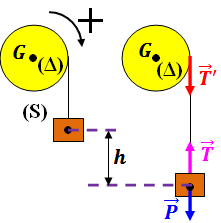
\includegraphics[width=0.7\linewidth]{images/PremierBac/p3/im3.png}}
\end{flushleft}
\end{minipage}
					\end{exercice}%===  ===%
  %Exercice 2
					\begin{exercice}{}/
					نعلق كرية صغيرة بنهاية خيط ، طوله
$L=50\ cm$				
					ثبت
		طرفه الآخر بحامل ثابت . نزيح الخيط و الكرية عن موضع
التوازن بزاوية
$\theta_{max} = 30^{\circ}$
ونتركها بدون سرعة بدئية.
\begin{enumerate}
\item بتطبيقك لمبرهنة الطاقة الحركية ، أوجد تعبير
$v$
سرعة الكرية عندما يكون الخيط زاوية
$\theta$
مع الخط الرأسي
بدلالة
$L$
و
$g$
 و
 $\theta$
  و
$\theta_{max}$.
مع
$g=10\ N.kg^{-1}$.
\item إستنتج سرعة الكرية عندما تمر بموضع توازنها.
\end{enumerate}
					\end{exercice}%===  ===%  
  %Exercice 2
					\begin{exercice}{}/
					يتكون نواس بسيط من كرية صغيرة كتلتها 
$m=500\ g$					
					ومن خيط طوله 
$L = 40\ cm$				
					وكتلته مهملة مثبت في النقطة 
$O$					
					بحامل أفقي .\\
					\begin{minipage}[c]{0.73\linewidth}
					ينحرف النواس بزاوية 
$\theta = 60^{\circ}$				
					عن موضع توازنه المستقر ثم يطلق بدون سرعة بدئية لينجز تذبذبات حول موضع توازنه.
					\begin{enumerate}
					\item أحسب شغل وزن الكرية عندما ينطلق النواس من الموضع 
$B$					
					نحو موضعه توازنه
$A$					
					\item ما هو شغل القوة
$\overrightarrow{T}$					
					المطبقة من طرف الخيط.علل جوابك.
					\item بتطبيقك لمبرهنة الطاقة الحركية على الكرية بين الموضعين 
$B$					
					و
$A$					
					أعط تعبير السرعة 
$v_A$					
					للكرية عند موضع التوازن.
					\end{enumerate}
\end{minipage}
					\begin{minipage}[c]{0.25\linewidth}
\psset{xunit=.5pt,yunit=.5pt,runit=.5pt}
\begin{flushleft}
\begin{adjustbox}{width=0.85\linewidth}
\fbox{\begin{pspicture}(196,253)
{
\newrgbcolor{curcolor}{0 0 0}
\pscustom[linestyle=none,fillstyle=solid,fillcolor=curcolor]
{
\newpath
\moveto(31,87)
\curveto(31,93.6)(36.4,99)(43,99)
\curveto(49.6,99)(55,93.6)(55,87)
\curveto(55,80.4)(49.6,75)(43,75)
\curveto(36.4,75)(31,80.4)(31,87)
\closepath
}
}
{
\newrgbcolor{curcolor}{0 0 0}
\pscustom[linewidth=2,linecolor=curcolor]
{
\newpath
\moveto(31,87)
\curveto(31,93.6)(36.4,99)(43,99)
\curveto(49.6,99)(55,93.6)(55,87)
\curveto(55,80.4)(49.6,75)(43,75)
\curveto(36.4,75)(31,80.4)(31,87)
\closepath
}
}
{
\newrgbcolor{curcolor}{0 0 0}
\pscustom[linewidth=3,linecolor=curcolor,linestyle=dashed,dash=2.5 2.5]
{
\newpath
\moveto(174.7,220)
\lineto(174.7,35)
}
}
{
\newrgbcolor{curcolor}{0 0 0}
\pscustom[linewidth=3.01227489,linecolor=curcolor]
{
\newpath
\moveto(43,88.3)
\lineto(175.202,220.502)
}
}
{
\newrgbcolor{curcolor}{0 0 0}
\pscustom[linewidth=1.67348936,linecolor=curcolor]
{
\newpath
\moveto(141.63,186.63)
\curveto(150.505,177.755)(162.433,172.785)(175,172.856)
\moveto(170.953,215.953)
\lineto(131.69,176.69)
\closepath
\moveto(175,214.036)
\lineto(175,158.798)
\closepath
}
}
{
\newrgbcolor{curcolor}{0 0 0}
\pscustom[linestyle=none,fillstyle=solid,fillcolor=curcolor]
{
\newpath
\moveto(175.03296875,234.864375)
\curveto(175.03296875,236.614375)(175.2946875,238.083125)(175.818125,239.270625)
\curveto(176.20875,240.145625)(176.74,240.93078125)(177.411875,241.62609375)
\curveto(178.0915625,242.32140625)(178.83375,242.83703125)(179.6384375,243.17296875)
\curveto(180.70875,243.62609375)(181.943125,243.85265625)(183.3415625,243.85265625)
\curveto(185.8728125,243.85265625)(187.89625,243.0675)(189.411875,241.4971875)
\curveto(190.9353125,239.926875)(191.69703125,237.74328125)(191.69703125,234.94640625)
\curveto(191.69703125,232.17296875)(190.943125,230.00109375)(189.4353125,228.43078125)
\curveto(187.9275,226.86828125)(185.911875,226.08703125)(183.3884375,226.08703125)
\curveto(180.83375,226.08703125)(178.8025,226.864375)(177.2946875,228.4190625)
\curveto(175.786875,229.9815625)(175.03296875,232.13)(175.03296875,234.864375)
\closepath
\moveto(178.6071875,234.9815625)
\curveto(178.6071875,233.03625)(179.05640625,231.5596875)(179.95484375,230.551875)
\curveto(180.85328125,229.551875)(181.99390625,229.051875)(183.37671875,229.051875)
\curveto(184.75953125,229.051875)(185.89234375,229.54796875)(186.77515625,230.54015625)
\curveto(187.66578125,231.54015625)(188.11109375,233.03625)(188.11109375,235.0284375)
\curveto(188.11109375,236.9971875)(187.6775,238.4659375)(186.8103125,239.4346875)
\curveto(185.9509375,240.4034375)(184.80640625,240.8878125)(183.37671875,240.8878125)
\curveto(181.94703125,240.8878125)(180.7946875,240.395625)(179.9196875,239.41125)
\curveto(179.0446875,238.4346875)(178.6071875,236.958125)(178.6071875,234.9815625)
\closepath
}
}
{
\newrgbcolor{curcolor}{0 0 0}
\pscustom[linewidth=3.34879403,linecolor=curcolor,linestyle=dashed,dash=2.5 2.5]
{
\newpath
\moveto(43,88.3)
\curveto(58.042,68.805)(111.201,34.495)(175.153,34.302)
}
}
{
\newrgbcolor{curcolor}{0 0 0}
\pscustom[linestyle=none,fillstyle=solid,fillcolor=curcolor]
{
\newpath
\moveto(6.2578125,93.6796875)
\lineto(13.125,93.6796875)
\curveto(14.484375,93.6796875)(15.49609375,93.62109375)(16.16015625,93.50390625)
\curveto(16.83203125,93.39453125)(17.4296875,93.16015625)(17.953125,92.80078125)
\curveto(18.484375,92.44140625)(18.92578125,91.9609375)(19.27734375,91.359375)
\curveto(19.62890625,90.765625)(19.8046875,90.09765625)(19.8046875,89.35546875)
\curveto(19.8046875,88.55078125)(19.5859375,87.8125)(19.1484375,87.140625)
\curveto(18.71875,86.46875)(18.1328125,85.96484375)(17.390625,85.62890625)
\curveto(18.4375,85.32421875)(19.2421875,84.8046875)(19.8046875,84.0703125)
\curveto(20.3671875,83.3359375)(20.6484375,82.47265625)(20.6484375,81.48046875)
\curveto(20.6484375,80.69921875)(20.46484375,79.9375)(20.09765625,79.1953125)
\curveto(19.73828125,78.4609375)(19.2421875,77.87109375)(18.609375,77.42578125)
\curveto(17.984375,76.98828125)(17.2109375,76.71875)(16.2890625,76.6171875)
\curveto(15.7109375,76.5546875)(14.31640625,76.515625)(12.10546875,76.5)
\lineto(6.2578125,76.5)
\closepath
\moveto(9.7265625,90.8203125)
\lineto(9.7265625,86.84765625)
\lineto(12,86.84765625)
\curveto(13.3515625,86.84765625)(14.19140625,86.8671875)(14.51953125,86.90625)
\curveto(15.11328125,86.9765625)(15.578125,87.1796875)(15.9140625,87.515625)
\curveto(16.2578125,87.859375)(16.4296875,88.30859375)(16.4296875,88.86328125)
\curveto(16.4296875,89.39453125)(16.28125,89.82421875)(15.984375,90.15234375)
\curveto(15.6953125,90.48828125)(15.26171875,90.69140625)(14.68359375,90.76171875)
\curveto(14.33984375,90.80078125)(13.3515625,90.8203125)(11.71875,90.8203125)
\closepath
\moveto(9.7265625,83.98828125)
\lineto(9.7265625,79.39453125)
\lineto(12.9375,79.39453125)
\curveto(14.1875,79.39453125)(14.98046875,79.4296875)(15.31640625,79.5)
\curveto(15.83203125,79.59375)(16.25,79.8203125)(16.5703125,80.1796875)
\curveto(16.8984375,80.546875)(17.0625,81.03515625)(17.0625,81.64453125)
\curveto(17.0625,82.16015625)(16.9375,82.59765625)(16.6875,82.95703125)
\curveto(16.4375,83.31640625)(16.07421875,83.578125)(15.59765625,83.7421875)
\curveto(15.12890625,83.90625)(14.10546875,83.98828125)(12.52734375,83.98828125)
\closepath
}
}
{
\newrgbcolor{curcolor}{0 0 0}
\pscustom[linestyle=none,fillstyle=solid,fillcolor=curcolor]
{
\newpath
\moveto(184.73828125,12)
\lineto(180.96484375,12)
\lineto(179.46484375,15.90234375)
\lineto(172.59765625,15.90234375)
\lineto(171.1796875,12)
\lineto(167.5,12)
\lineto(174.19140625,29.1796875)
\lineto(177.859375,29.1796875)
\closepath
\moveto(178.3515625,18.796875)
\lineto(175.984375,25.171875)
\lineto(173.6640625,18.796875)
\closepath
}
}
{
\newrgbcolor{curcolor}{0 0 0}
\pscustom[linewidth=4,linecolor=curcolor]
{
\newpath
\moveto(45.7,15)
\lineto(45.7,87)
}
}
{
\newrgbcolor{curcolor}{0 0 0}
\pscustom[linewidth=4,linecolor=curcolor]
{
\newpath
\moveto(51.7,23)
\lineto(45.7,11)
\lineto(39.7,23)
}
}
{
\newrgbcolor{curcolor}{0 0 0}
\pscustom[linewidth=4.01636652,linecolor=curcolor]
{
\newpath
\moveto(91.16,136.16)
\lineto(50.832,95.832)
}
}
{
\newrgbcolor{curcolor}{0 0 0}
\pscustom[linewidth=4.01636652,linecolor=curcolor]
{
\newpath
\moveto(81.22,134.74)
\lineto(94,139)
\lineto(89.74,126.22)
}
}
{
\newrgbcolor{curcolor}{0 0 0}
\pscustom[linestyle=none,fillstyle=solid,fillcolor=curcolor]
{
\newpath
\moveto(51.61328125,126)
\lineto(51.61328125,140.2734375)
\lineto(46.515625,140.2734375)
\lineto(46.515625,143.1796875)
\lineto(60.16796875,143.1796875)
\lineto(60.16796875,140.2734375)
\lineto(55.08203125,140.2734375)
\lineto(55.08203125,126)
\closepath
}
}
{
\newrgbcolor{curcolor}{0 0 0}
\pscustom[linestyle=none,fillstyle=solid,fillcolor=curcolor]
{
\newpath
\moveto(58.66536408,150.08333319)
\lineto(44.68359373,150.08333319)
\lineto(44.68359373,150.96744775)
\lineto(58.66536408,150.96744775)
\curveto(57.80251689,151.96397549)(57.19791622,152.73263866)(56.85156206,153.27343725)
\curveto(56.50520791,153.82031223)(56.16796834,154.49782957)(55.83984335,155.30598927)
\lineto(56.56900999,155.30598927)
\curveto(57.27994746,154.4309893)(58.16406202,153.54383655)(59.22135365,152.64453102)
\curveto(60.27864528,151.7452255)(61.11718692,151.11935746)(61.73697856,150.76692692)
\lineto(61.73697856,150.25651027)
\curveto(60.92881887,149.80685751)(60.04470431,149.16276031)(59.0846349,148.32421867)
\curveto(58.13064188,147.48567703)(57.29210024,146.62586803)(56.56900999,145.74479168)
\lineto(55.83984335,145.74479168)
\curveto(56.1861975,146.56510415)(56.54166624,147.26085065)(56.90624956,147.83203119)
\curveto(57.27083288,148.40321172)(57.85720439,149.15364573)(58.66536408,150.08333319)
\closepath
}
}
{
\newrgbcolor{curcolor}{0 0 0}
\pscustom[linestyle=none,fillstyle=solid,fillcolor=curcolor]
{
\newpath
\moveto(21.24609375,35)
\lineto(21.24609375,52.1796875)
\lineto(26.8125,52.1796875)
\curveto(28.921875,52.1796875)(30.296875,52.09375)(30.9375,51.921875)
\curveto(31.921875,51.6640625)(32.74609375,51.1015625)(33.41015625,50.234375)
\curveto(34.07421875,49.375)(34.40625,48.26171875)(34.40625,46.89453125)
\curveto(34.40625,45.83984375)(34.21484375,44.953125)(33.83203125,44.234375)
\curveto(33.44921875,43.515625)(32.9609375,42.94921875)(32.3671875,42.53515625)
\curveto(31.78125,42.12890625)(31.18359375,41.859375)(30.57421875,41.7265625)
\curveto(29.74609375,41.5625)(28.546875,41.48046875)(26.9765625,41.48046875)
\lineto(24.71484375,41.48046875)
\lineto(24.71484375,35)
\closepath
\moveto(24.71484375,49.2734375)
\lineto(24.71484375,44.3984375)
\lineto(26.61328125,44.3984375)
\curveto(27.98046875,44.3984375)(28.89453125,44.48828125)(29.35546875,44.66796875)
\curveto(29.81640625,44.84765625)(30.17578125,45.12890625)(30.43359375,45.51171875)
\curveto(30.69921875,45.89453125)(30.83203125,46.33984375)(30.83203125,46.84765625)
\curveto(30.83203125,47.47265625)(30.6484375,47.98828125)(30.28125,48.39453125)
\curveto(29.9140625,48.80078125)(29.44921875,49.0546875)(28.88671875,49.15625)
\curveto(28.47265625,49.234375)(27.640625,49.2734375)(26.390625,49.2734375)
\closepath
}
}
{
\newrgbcolor{curcolor}{0 0 0}
\pscustom[linestyle=none,fillstyle=solid,fillcolor=curcolor]
{
\newpath
\moveto(33.67536408,60.58333319)
\lineto(19.69359373,60.58333319)
\lineto(19.69359373,61.46744775)
\lineto(33.67536408,61.46744775)
\curveto(32.81251689,62.46397549)(32.20791622,63.23263866)(31.86156206,63.77343725)
\curveto(31.51520791,64.32031223)(31.17796834,64.99782957)(30.84984335,65.80598927)
\lineto(31.57900999,65.80598927)
\curveto(32.28994746,64.9309893)(33.17406202,64.04383655)(34.23135365,63.14453102)
\curveto(35.28864528,62.2452255)(36.12718692,61.61935746)(36.74697856,61.26692692)
\lineto(36.74697856,60.75651027)
\curveto(35.93881887,60.30685751)(35.05470431,59.66276031)(34.0946349,58.82421867)
\curveto(33.14064188,57.98567703)(32.30210024,57.12586803)(31.57900999,56.24479168)
\lineto(30.84984335,56.24479168)
\curveto(31.1961975,57.06510415)(31.55166624,57.76085065)(31.91624956,58.33203119)
\curveto(32.28083288,58.90321172)(32.86720439,59.65364573)(33.67536408,60.58333319)
\closepath
}
}
{
\newrgbcolor{curcolor}{0 0 0}
\pscustom[linestyle=none,fillstyle=solid,fillcolor=curcolor]
{
\newpath
\moveto(140.90296875,152.17578125)
\curveto(140.90296875,155.25390625)(141.52796875,157.625)(142.77796875,159.2890625)
\curveto(143.72328125,160.5390625)(144.85609375,161.1640625)(146.17640625,161.1640625)
\curveto(147.45765625,161.1640625)(148.55140625,160.5625)(149.45765625,159.359375)
\curveto(150.72328125,157.6796875)(151.35609375,155.39453125)(151.35609375,152.50390625)
\curveto(151.35609375,149.75390625)(150.735,147.58203125)(149.4928125,145.98828125)
\curveto(148.5240625,144.75390625)(147.3834375,144.13671875)(146.0709375,144.13671875)
\curveto(145.36,144.13671875)(144.7115625,144.30859375)(144.125625,144.65234375)
\curveto(143.5396875,144.99609375)(143.02015625,145.4921875)(142.56703125,146.140625)
\curveto(142.11390625,146.7890625)(141.76625,147.4765625)(141.5240625,148.203125)
\curveto(141.11,149.453125)(140.90296875,150.77734375)(140.90296875,152.17578125)
\closepath
\moveto(149.094375,153.0078125)
\curveto(149.0865625,155.046875)(148.89125,156.68359375)(148.5084375,157.91796875)
\curveto(148.2115625,158.86328125)(147.81703125,159.5390625)(147.32484375,159.9453125)
\curveto(146.96546875,160.2421875)(146.55140625,160.390625)(146.08265625,160.390625)
\curveto(145.55140625,160.390625)(145.063125,160.18359375)(144.6178125,159.76953125)
\curveto(144.1725,159.35546875)(143.83265625,158.6640625)(143.59828125,157.6953125)
\curveto(143.37171875,156.7265625)(143.219375,155.1640625)(143.14125,153.0078125)
\closepath
\moveto(143.14125,152.234375)
\curveto(143.1725,150.84375)(143.27796875,149.59375)(143.45765625,148.484375)
\curveto(143.59046875,147.640625)(143.8209375,146.90625)(144.1490625,146.28125)
\curveto(144.344375,145.90625)(144.62953125,145.5859375)(145.00453125,145.3203125)
\curveto(145.37953125,145.0625)(145.781875,144.93359375)(146.2115625,144.93359375)
\curveto(146.7115625,144.93359375)(147.18421875,145.16796875)(147.62953125,145.63671875)
\curveto(148.08265625,146.10546875)(148.4225,146.859375)(148.6490625,147.8984375)
\curveto(148.8834375,148.9375)(149.0240625,150.3828125)(149.0709375,152.234375)
\closepath
}
}
\end{pspicture}}
\end{adjustbox}
\end{flushleft}
					\end{minipage} 
					\end{exercice}%===  ===%  
  
\end{document}